% Classicthesis Typographic Thesis
% LaTeX Template
% Version 1.4 (1/1/16)
%
% This template has been downloaded from:
% http://www.LaTeXTemplates.com
%
% Original author:
% André Miede (http://www.miede.de) with commenting modifications by:
% Vel (vel@LaTeXTemplates.com)
%
% License:
% GNU General Public License (v2)
%
% General Tips:
% 1) Make sure to edit the classicthesis-config.file
% 2) New enumeration (A., B., C., etc in small caps): \begin{aenumerate} \end{aenumerate}
% 3) For margin notes: \marginpar or \graffito{}
% 4) Do not use bold fonts in this style, it is designed around them
% 5) Use tables as in the examples
% 6) See classicthesis-preamble.sty for useful commands
%
%%%%%%%%%%%%%%%%%%%%%%%%%%%%%%%%%%%%%%%%%

%----------------------------------------------------------------------------------------
%	PACKAGES AND OTHER DOCUMENT CONFIGURATIONS
%----------------------------------------------------------------------------------------

\newif\ifnotes
\notestrue
%\notesfalse 

\documentclass[
		twoside,openright,titlepage,numbers=noenddot,headinclude,%1headlines,
	 	footinclude=true,cleardoublepage=empty,
		dottedtoc, % Make page numbers in the table of contents flushed right with dots leading to them
		BCOR=5mm,paper=a4,fontsize=11pt, % Binding correction, paper type and font size
		ngerman,american, % Languages, change this to your language(s)
		]{scrreprt} 
                

% Includes the file which contains all the document configurations and packages - make sure to edit this file
%%%%%%%%%%%%%%%%%%%%%%%%%%%%%%%%%%%%%%%%%
% Classicthesis Typographic Thesis
% Configuration File
%
% This file has been downloaded from:
% http://www.LaTeXTemplates.com
%
% Original author:
% André Miede (http://www.miede.de) with extensive commenting changes by:
% Vel (vel@LaTeXTemplates.com)
%
% License:
% GNU General Public License (v2)
%
% Important note:
% The main lines to change in this file are in the DOCUMENT VARIABLES
% section, the rest of the file is for advanced configuration.
%
%%%%%%%%%%%%%%%%%%%%%%%%%%%%%%%%%%%%%%%%%

%----------------------------------------------------------------------------------------
%	CHARACTER ENCODING
%----------------------------------------------------------------------------------------

\PassOptionsToPackage{utf8}{inputenc} % Set the encoding of your files. UTF-8 is the only sensible encoding nowadays. If you can't read äöüßáéçèê∂åëæƒÏ€ then change the encoding setting in your editor, not the line below. If your editor does not support utf8 use another editor!
\usepackage{inputenc}

%----------------------------------------------------------------------------------------
%	DOCUMENT VARIABLES
%	Fill in the lines below to enter your information into the thesis template
%	Each of the commands can be cited anywhere in the thesis
%----------------------------------------------------------------------------------------

% Remove drafting to get rid of the '[ Date - classicthesis version 4.0 ]' text at the bottom of every page
\PassOptionsToPackage{eulerchapternumbers,listings, pdfspacing, subfig,beramono,eulermath,parts}{classicthesis}
% Available options: drafting parts nochapters linedheaders eulerchapternumbers beramono eulermath pdfspacing minionprospacing tocaligned dottedtoc manychapters listings floatperchapter subfig

\newcommand{\myTitle}{The Practice of Change\xspace}
\newcommand{\mySubtitle}{How I survived being interested in everything\xspace}
\newcommand{\myDegree}{Doctoral Dissertation\xspace}
\newcommand{\myName}{Joichi Ito\xspace}
\newcommand{\myProf}{Jun Murai\xspace}
\newcommand{\myOtherProf}{Put name here\xspace}
\newcommand{\mySupervisor}{Jun Murai\xspace}
\newcommand{\myFaculty}{Thesis Supervisor\xspace}
\newcommand{\myDepartment}{Graduate School of Media \& Governance\xspace}
\newcommand{\myUni}{Keio University\xspace}
\newcommand{\myLocation}{Cambridge, MA\xspace}
\newcommand{\myTime}{2018\xspace}
\newcommand{\myVersion}{(Draft)\xspace}
\newcommand{\myTimestamp}{\DTMnow\xspace}

%----------------------------------------------------------------------------------------
%	USEFUL COMMANDS
%----------------------------------------------------------------------------------------

\newcommand{\ie}{i.\,e.}
\newcommand{\Ie}{I.\,e.}
\newcommand{\eg}{e.\,g.}
\newcommand{\Eg}{E.\,g.} 

\newcounter{dummy} % Necessary for correct hyperlinks (to index, bib, etc.)
\providecommand{\mLyX}{L\kern-.1667em\lower.25em\hbox{Y}\kern-.125emX\@}
\newlength{\abcd} % for ab..z string length calculation

%----------------------------------------------------------------------------------------
%	PACKAGES
%----------------------------------------------------------------------------------------

\usepackage{lipsum} % Used for inserting dummy 'Lorem ipsum' text into the template
\usepackage{ccicons}
\usepackage{datetime2}
%\usepackage{wasysym}
\usepackage{soul} %\ to use \hl{}

%------------------------------------------------

%\PassOptionsToPackage{ngerman,american}{babel}  % Change this to your language(s)
% Spanish languages need extra options in order to work with this template
%\PassOptionsToPackage{spanish,es-lcroman}{babel}
\usepackage{babel}

%------------------------------------------------			

\usepackage{csquotes}
\PassOptionsToPackage{%
%backend=biber, % Instead of bibtex
backend=bibtex8,bibencoding=ascii,%
language=auto,%
%style=apalike,%
style=authoryear-comp, % Author 1999, 2010
bibstyle=authoryear,dashed=false, % dashed: substitute rep. author with ---
sorting=nyt, % name, year, title
maxbibnames=10, % default: 3, et al.
backref=true,%
autocite=inline,
natbib=true % natbib compatibility mode (\citep and \citet still work)
}{biblatex}
\usepackage[backend=biber]{biblatex}
\usepackage{letltxmacro}\LetLtxMacro{\cite}{\parencite}
 
 %------------------------------------------------

\PassOptionsToPackage{fleqn}{amsmath} % Math environments and more by the AMS 
 \usepackage{amsmath}
 
 %------------------------------------------------

\PassOptionsToPackage{T1}{fontenc} % T2A for cyrillics
\usepackage{fontenc}

%------------------------------------------------

\usepackage{textcomp} % Fix warning with missing font shapes

%------------------------------------------------

\usepackage{scrhack} % Fix warnings when using KOMA with listings package  

%------------------------------------------------

\usepackage{xspace} % To get the spacing after macros right

%------------------------------------------------

\usepackage{mparhack} % To get marginpar right

%------------------------------------------------

\usepackage{fixltx2e} % Fixes some LaTeX stuff 

%------------------------------------------------

\PassOptionsToPackage{smaller}{acronym} % Include printonlyused in the first bracket to only show acronyms used in the text
\usepackage{acronym} % Nice macros for handling all acronyms in the thesis

%\renewcommand*{\acsfont}[1]{\textssc{#1}} % For MinionPro
\renewcommand*{\aclabelfont}[1]{\acsfont{#1}}

%------------------------------------------------

\PassOptionsToPackage{pdftex}{graphicx}
\usepackage{graphicx} 

%----------------------------------------------------------------------------------------
%	FLOATS: TABLES, FIGURES AND CAPTIONS SETUP
%----------------------------------------------------------------------------------------

\usepackage{tabularx} % Better tables
\setlength{\extrarowheight}{3pt} % Increase table row height
\newcommand{\tableheadline}[1]{\multicolumn{1}{c}{\spacedlowsmallcaps{#1}}}
\newcommand{\myfloatalign}{\centering} % To be used with each float for alignment
\usepackage{caption}
\captionsetup{font=small}
\usepackage{subfig}  

%----------------------------------------------------------------------------------------
%	CODE LISTINGS SETUP
%----------------------------------------------------------------------------------------

\usepackage{listings} 
%\lstset{emph={trueIndex,root},emphstyle=\color{BlueViolet}}%\underbar} % For special keywords
\lstset{language=[LaTeX]Tex,%C++ % Specify the language(s) for listings here
morekeywords={PassOptionsToPackage,selectlanguage},
keywordstyle=\color{RoyalBlue}, % Add \bfseries for bold
basicstyle=\small\ttfamily, % Makes listings a smaller font size and a different font
%identifierstyle=\color{NavyBlue}, % Color of text inside brackets
commentstyle=\color{Green}\ttfamily, % Color of comments
stringstyle=\rmfamily, % Font type to use for strings
numbers=left, % Change left to none to remove line numbers
numberstyle=\scriptsize, % Font size of the line numbers
stepnumber=5, % Increment of line numbers
numbersep=8pt, % Distance of line numbers from code listing
showstringspaces=false, % Sets whether spaces in strings should appear underlined
breaklines=true, % Force the code to stay in the confines of the listing box
%frameround=ftff, % Uncomment for rounded frame
%frame=single, % Frame border - none/leftline/topline/bottomline/lines/single/shadowbox/L
belowcaptionskip=.75\baselineskip % Space after the "Listing #: Desciption" text and the listing box
}

%----------------------------------------------------------------------------------------
%	HYPERREFERENCES
%----------------------------------------------------------------------------------------

\PassOptionsToPackage{hyperfootnotes=false,pdfpagelabels}{hyperref}
\usepackage[driverfallback=dvipdfmx]{hyperref}  % backref linktocpage pagebackref
%\pdfcompresslevel=0
%\pdfadjustspacing=1

\hypersetup{
% Uncomment the line below to remove all links (to references, figures, tables, etc), useful for b/w printouts
%draft, 
colorlinks=true, linktocpage=true, pdfstartpage=3, pdfstartview=FitV,
% Uncomment the line below if you want to have black links (e.g. for printing black and white)
%colorlinks=false, linktocpage=false, pdfborder={0 0 0}, pdfstartpage=3, pdfstartview=FitV, 
breaklinks=true, pdfpagemode=UseNone, pageanchor=true, pdfpagemode=UseOutlines,%
plainpages=false, bookmarksnumbered, bookmarksopen=true, bookmarksopenlevel=1,%
hypertexnames=true, pdfhighlight=/O,%nesting=true,%frenchlinks,%
urlcolor=webbrown, linkcolor=RoyalBlue, citecolor=webgreen, %pagecolor=RoyalBlue,%
    %urlcolor=Black, linkcolor=Black, citecolor=Black, %pagecolor=Black,%
%------------------------------------------------
% PDF file meta-information 
pdftitle={\myTitle},
pdfauthor={\textcopyright\ \myName, \myUni, \myFaculty},
pdfsubject={},
pdfkeywords={},
pdfcreator={pdfLaTeX},
pdfproducer={LaTeX with hyperref and classicthesis}
%------------------------------------------------
}

%----------------------------------------------------------------------------------------
%	AUTOREFERENCES SETUP
%	Redefines how references in text are prefaced for different 
%	languages (e.g. "Section 1.2" or "section 1.2")
%----------------------------------------------------------------------------------------

\makeatletter
\@ifpackageloaded{babel}
{
\addto\extrasamerican{
\renewcommand*{\figureautorefname}{Figure}
\renewcommand*{\tableautorefname}{Table}
\renewcommand*{\partautorefname}{Part}
\renewcommand*{\chapterautorefname}{Chapter}
\renewcommand*{\sectionautorefname}{Section}
\renewcommand*{\subsectionautorefname}{Section}
\renewcommand*{\subsubsectionautorefname}{Section}
}
\addto\extrasngerman{
\renewcommand*{\paragraphautorefname}{Absatz}
\renewcommand*{\subparagraphautorefname}{Unterabsatz}
\renewcommand*{\footnoteautorefname}{Fu\"snote}
\renewcommand*{\FancyVerbLineautorefname}{Zeile}
\renewcommand*{\theoremautorefname}{Theorem}
\renewcommand*{\appendixautorefname}{Anhang}
\renewcommand*{\equationautorefname}{Gleichung}
\renewcommand*{\itemautorefname}{Punkt}
}
\providecommand{\subfigureautorefname}{\figureautorefname} % Fix to getting autorefs for subfigures right
}{\relax}
\makeatother

%----------------------------------------------------------------------------------------

\usepackage{classicthesis} 



%----------------------------------------------------------------------------------------
%	CHANGING TEXT AREA 
%----------------------------------------------------------------------------------------

%\linespread{1.05} % a bit more for Palatino
%\areaset[current]{312pt}{761pt} % 686 (factor 2.2) + 33 head + 42 head \the\footskip
%\setlength{\marginparwidth}{7em}%
%\setlength{\marginparsep}{2em}%

%----------------------------------------------------------------------------------------
%	USING DIFFERENT FONTS
%----------------------------------------------------------------------------------------

%\usepackage[oldstylenums]{kpfonts} % oldstyle notextcomp
%\usepackage[osf]{libertine}
%\usepackage[light,condensed,math]{iwona}
%\renewcommand{\sfdefault}{iwona}
%\usepackage{lmodern} % <-- no osf support :-(
%\usepackage{cfr-lm} % 
%\usepackage[urw-garamond]{mathdesign} <-- no osf support :-(
%\usepackage[default,osfigures]{opensans} % scale=0.95 
%\usepackage[sfdefault]{FiraSans}


\addbibresource{Bibliography.bib} % The file housing your bibliography
%\addbibresource[label=ownpubs]{Self_Publications.bib} % Uncomment for optional self-publications

%\hyphenation{Put special hyphenation here}

\begin{document}

% commenting macros
\ifnotes
  \newcommand{\colornote}[3]{\textcolor{#1}{\smaller\sffamily\bfseries\boldmath[\ignorespaces #2 --- \smaller\textit{#3}]}}
\else
  \newcommand{\colornote}[3]{}
\fi
\newcommand{\dw}[1]{\colornote{red}{#1}{David Weinberger}}
\newcommand{\joi}[1]{\colornote{cyan}{#1}{Joi}}


% Don't show comments 
\renewcommand{\dw}[1]{}
\renewcommand{\joi}[1]{}

\frenchspacing % Reduces space after periods to make text more compact

\raggedbottom % Makes all pages the height of the text on that page

\selectlanguage{american} % Select your default language - e.g. american or ngerman

%\renewcommand*{\bibname}{new name} % Uncomment to change the name of the bibliography
%\setbibpreamble{} % Uncomment to include a preamble to the bibliography - some text before the reference list starts

\pagenumbering{roman} % Roman page numbering prior to the start of the thesis content (i, ii, iii, etc)

\pagestyle{plain} % Suppress headers for the pre-content pages

%----------------------------------------------------------------------------------------
%	PRE-CONTENT THESIS PAGES
%----------------------------------------------------------------------------------------

% Title Page

\begin{titlepage}

\begin{addmargin}[-1cm]{-3cm}
\begin{center}
\large


\spacedlowsmallcaps{\myDegree} \\
\spacedlowsmallcaps{Academic Year \myTime} \\
\vfill

\begingroup
 \color{Maroon}\spacedallcaps{\myTitle} \\ \bigskip % Thesis title
\endgroup

\vfill

\spacedlowsmallcaps{\myUni} \\
\spacedlowsmallcaps{\myDepartment} \\ \bigskip

\spacedlowmediumcaps{\myName} \\ 
\spacedlowsmallcaps{\myVersion} \\
% \spacedlowsmallcaps{\myTimestamp}
\end{center}

% Your name
% \spacedlowsmallcaps{\mySupervisor} \\
% \spacedlowsmallcaps{\myFaculty} \\
%  \bigskip
 
% \vfill

% \begin{center}

% \end{center}
\end{addmargin}

\end{titlepage}
 % Main title page

% Back of the title page

\thispagestyle{empty}

\hfill

\vfill

\noindent\myName: \textit{\myTitle,} \mySubtitle, %\myDegree, 
\textcopyright\ \myTime  \ccby 

% You may wish to do something with the back of the title page, such as including your supervisors, location or time frame of the work. Below is an example of doing so although you may want to tweak it to your liking.

%\bigskip

%\noindent\spacedlowsmallcaps{Supervisors}: \\
%\myProf \\
%\myOtherProf \\ 
%\mySupervisor

%\medskip \\

%\noindent\spacedlowsmallcaps{Location}: \\
%\myLocation

%\medskip \\

%\noindent\spacedlowsmallcaps{Time Frame}: \\
%\myTime
 % Back of the title page

% \cleardoublepage% Dedication

\thispagestyle{empty}
\refstepcounter{dummy}

\pdfbookmark[1]{Dedication}{Dedication} % Bookmark name visible in a PDF viewer

\vspace*{3cm}

\medskip

\begin{center}
Dedicated to my mother who loved me regardless of who I was but encouraged me to be the best that I can be.
\end{center} % Dedication page

\cleardoublepage% Abstract

%\renewcommand{\abstractname}{Abstract} % Uncomment to change the name of the abstract

\pdfbookmark[1]{Abstract}{Abstract} % Bookmark name visible in a PDF viewer

\begingroup
\let\clearpage\relax
\let\cleardoublepage\relax
\let\cleardoublepage\relax

\chapter*{Abstract}

Over the last century civilization has systematically supported a market-based approach to developing technical, financial, social and legal tools that focus on efficiency, growth and productivity. In this manner we have achieved considerable progress on some of the most pressing humanitarian challenges, such as eradicating infectious diseases and making life easier and more convenient. However, we have often put our tools and methods of use with little regard to their systemic or long-term effects, and have thereby created a set of new, interconnected, and more complex problems. Our new problems require new approaches: new understanding, solution design and intervention. Yet we continue to try to solve these new problems with the same tools that caused them.

\medskip

Therefore in my dissertation I ask:

\begin{center}
\textit{How can we understand and effectively intervene in\\
interconnected complex adaptive systems?}

\end{center}

In particular, my thesis presents through theory and practice the following contributions to addressing these problems:

\begin{enumerate}
\item \textbf{A post-Internet framework for understanding and intervening in complex adaptive systems.} Drawing on systems dynamics, evolutionary dynamics and theory of change based on causal networks, I describe a way to understand and suggest ways to intervene in complex systems. I argue that an anti-disciplinary approach and paradigm shifts are required to achieve the outcomes we desire.
\item \textbf{Learnings from the creation and management of post-Internet organizations that can be applied to designing and deploying interventions.} I propose an architecture of layers of interoperability to unbundle complex, inflexible, and monolithic systems and increase competition, cooperation, generativity, and flexibility. I argue that the Internet is the best example of this architecture and that the Internet has provided an opportunity to deploy this architecture in other domains. I demonstrate how the Internet has has made the world more complex but through lowering the cost of communication and collaboration has enabled new forms of organization and production. This has changed the nature of our interventions.
\item \textbf{How and why we must change the values of society from one based on the measurement of financial value to flourishing and robustness.} The paradigm determines what we measure and generates the values and the goals of a system. Measuring value financially has created a competitive market-based system that has provided many societal benefits but has produced complex problems not solvable through competitive market-based solutions. In order to address these challenges, we must shift the paradigm across our systems to focus on a more complex measure of flourishing and robustness. In order to transcend our current economic paradigm, the transformation will require a movement that includes arts and culture to transform strongly held beliefs. I propose a framework of values based on the pursuit of flourishing and a method for transforming ourselves.
\end{enumerate}

Reflecting on my work experience, I examine my successes and failures in the form of learnings and insights. I discuss what questions are outstanding and conclude with a call to action with a theory of change; we need to bring about a fundamental normative shift in society through communities, away from the pursuit of growth for growth's sake and towards a sustainable sensibility of flourishing that can draw on both the historical examples and the sensibilities of some modern indigenous cultures, as well as new values emerging from theoretical and practical progress in science.

\vfill

Keywords: Cybernetics, Systems Dynamics, Philosophy of Science, Internet, Cryptocurrency

\endgroup % Abstract page

\cleardoublepage% Acknowledgements

\pdfbookmark[1]{Acknowledgements}{Acknowledgements} % Bookmark name visible in a PDF viewer



\begin{center}
  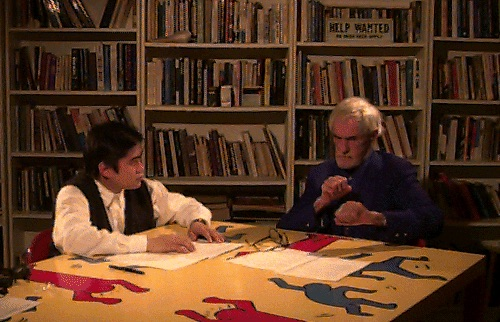
\includegraphics[width=.5\textwidth]{pictures/timleary.jpg}
  \\
  Scheming with Timothy Leary in 1995
\end{center}


\begin{flushright}{\slshape    
Question authority and think for yourself.  \\ \medskip
--- Timothy Leary}
\end{flushright}

\bigskip

%----------------------------------------------------------------------------------------

\begingroup

\let\clearpage\relax
\let\cleardoublepage\relax
\let\cleardoublepage\relax

\chapter*{Acknowledgements}

\noindent

To my late godfather Timothy Leary for ``Question Authority and Think For Yourself.''

To Jun Murai for pushing me to do this dissertation.

To my thesis advisors: Hiroya Tanaka, Rodney D. Van Meter, Keiko Okawa and Jonathan L. Zittrain for their extensive feedback, guidance and encouragement. 

To Nicholas Negroponte for the Media Lab and his mentorship.

To the late Kenichi Fukui for encouraging me to think about complex systems and the limits of reduction.

To the late John Perry Barlow for the ``Declaration of Independence of Cyberspace.''

To Hashim Sarkis for sending me in the direction of Foucault.

To Martin Nowak for his guidance on Evolutionary Dynamics.

To my colleagues at MIT and particularly at the Media Lab for continuous inspiration and my raison d'être.

To my research colleagues Karthik Dinakar, Chia Evers, Natalie Saltiel, Pratik Shah, and Andre Uhl for helping me with everything including this thesis.

To Yuka Sasaki, Stephanie Strom and Mika Tanaka for their help on helping me pull this dissertation together.

To David Weinberger for ``The final edit.''

To Sean Bonner, Danese Cooper, Ariel Ekblaw, Pieter Franken, Mizuko Ito, Mike Linksvayer, Pip Mothersill, Diane Peters, Deb Roy and Jeffrey Shapard for their feedback on various parts of the dissertation.

Finally, thanks to Kio and Mizuka for making room in our family life to work on this and for supporting me through the process.\\



\endgroup % Acknowledgements page

\pagestyle{scrheadings} % Show chapter titles as headings

\cleardoublepage% Table of Contents - List of Tables/Figures/Listings and Acronyms

\refstepcounter{dummy}

\pdfbookmark[1]{\contentsname}{tableofcontents} % Bookmark name visible in a PDF viewer

\setcounter{tocdepth}{2} % Depth of sections to include in the table of contents - currently up to subsections

\setcounter{secnumdepth}{3} % Depth of sections to number in the text itself - currently up to subsubsections

\manualmark
\markboth{\spacedlowsmallcaps{\contentsname}}{\spacedlowsmallcaps{\contentsname}}
\tableofcontents 
\automark[section]{chapter}
\renewcommand{\chaptermark}[1]{\markboth{\spacedlowsmallcaps{#1}}{\spacedlowsmallcaps{#1}}}
\renewcommand{\sectionmark}[1]{\markright{\thesection\enspace\spacedlowsmallcaps{#1}}}

\clearpage

\begingroup 
\let\clearpage\relax
\let\cleardoublepage\relax
\let\cleardoublepage\relax

%----------------------------------------------------------------------------------------
%	List of Figures
%----------------------------------------------------------------------------------------

\refstepcounter{dummy}
%\addcontentsline{toc}{chapter}{\listfigurename} % Uncomment if you would like the list of figures to appear in the table of contents
\pdfbookmark[1]{\listfigurename}{lof} % Bookmark name visible in a PDF viewer

\listoffigures

\vspace{8ex}
\newpage

%----------------------------------------------------------------------------------------
%	List of Tables
%----------------------------------------------------------------------------------------

\refstepcounter{dummy}
%\addcontentsline{toc}{chapter}{\listtablename} % Uncomment if you would like the list of tables to appear in the table of contents
\pdfbookmark[1]{\listtablename}{lot} % Bookmark name visible in a PDF viewer

\listoftables
        
\vspace{8ex}
\newpage
    
%----------------------------------------------------------------------------------------
%	List of Listings
%---------------------------------------------------------------------------------------- 

% \refstepcounter{dummy}
%\addcontentsline{toc}{chapter}{\lstlistlistingname} % Uncomment if you would like the list of listings to appear in the table of contents
% \pdfbookmark[1]{\lstlistlistingname}{lol} % Bookmark name visible in a PDF viewer

%\lstlistoflistings 

% \vspace{8ex}
% \newpage
       
%----------------------------------------------------------------------------------------
%	Acronyms
%----------------------------------------------------------------------------------------

 \refstepcounter{dummy}
\addcontentsline{toc}{chapter}{Acronyms} % Uncomment if you would like the acronyms to appear in the table of contents
 \pdfbookmark[1]{Acronyms}{acronyms} % Bookmark name visible in a PDF viewer

 \markboth{\spacedlowsmallcaps{Acronyms}}{\spacedlowsmallcaps{Acronyms}}

\chapter*{Acronyms}

\begin{acronym}[UML]
\acro{AI}{Artificial Intelligence}
\acro{ASIJ}{American School in Japan}
\acro{AIDS}{acquired immune deficiency syndrome}
\acro{AWG}{Air Quality Working Group}
\acro{API}{Application Programming Interface}
\acro{AeroAstro}{Department of Aeronautics and Astronautics}
\acro{BOJ}{The Bank of Japan}
\acro{CALEA}{Communications Assistance for Law Enforcement Act}
\acro{CC}{Creative Commons}
\acro{CERN}{\textit{Conseil européen pour la recherche nucléaire} [The European Organization for Nuclear Research]}
\acro{CIA}{Central Intelligence Agency}
\acro{DARPA}{The Defense Advanced Research Projects Agency}
\acro{DCI}{Digital Currency Initiative}
\acro{DNN}{deep neural network}
\acro{DRM}{Digital Rights Management}
\acro{EAPS}{Department of Earth, Atmospheric and Planetary Sciences}
\acro{EI}{Extended Intelligence}
\acro{FTP}{File Transfer Protocol}
\acro{GPL}{GNU General Public License}
\acro{GSA}{General Services Administration}
\acro{HTML}{HyperText Markup Language}
\acro{$IC_{50}$}{Half Maximal Inhibitory Concentration}
\acro{ICANN}{Internet Corporation for Assigned Names and Numbers}
\acro{IEEE}{The Institute of Electrical and Electronic Engineers}
\acro{IETF}{The Internet Engineering Task Force}
\acro{IMF}{International Monetary Fund}
\acro{IRC}{Internet Relay Chat}
\acro{ISS}{International Space Station}
\acro{JoDS}{Journal of Design and Science}
\acro{JPIX}{Japan Internet Exchange}
\acro{KFG}{Knowledge Futures Group}
\acro{MBA}{Master of Business Administration}
\acro{NASA}{National Aeronautics and Space Administration}
\acro{NCC}{New Context Conference}
\acro{NGO}{Non-governmental organization}
\acro{NTT}{Nippon Telephone and Telegraph}
\acro{OSI}{Open Source Initiative}
\acro{PCB}{Printed Circuit Board}
\acro{PI}{principal investigator}
\acro{RDF}{Resource Description Framework}
\acro{RSS}{Rich Site Summary; originally RDF Site Summary; often called Really Simple Syndication}
\acro{STEAM}{Science, Technology, Engineering and Math}
\acro{TCP/IP}{Transmission Control Protocol/Internet Protocol}
\acro{TEPCO}{Tokyo Electric Power Company}
\acro{VoIP}{Voice over Internet Protocol}
\acro{URL}{Uniform Resource Locator}
\acro{WAN}{wide area network}
\acro{WIDE}{Widely Integrated Distributed Environment}
\acro{X.25}{The International Telecommunication Union Telecommunication Standardization Sector standard protocol suite for packet switched wide area network communication}
\end{acronym}
                   
\endgroup % Contents, list of figures/tables/listings and acronyms

\cleardoublepage

\pagenumbering{arabic} % Arabic page numbering for thesis content (1, 2, 3, etc)
%\setcounter{page}{90} % Uncomment to manually start the page counter at an arbitrary value (for example if you wish to count the pre-content pages in the page count)

\cleardoublepage % Avoids problems with pdfbookmark

%----------------------------------------------------------------------------------------
%	THESIS CONTENT - CHAPTERS
%----------------------------------------------------------------------------------------

%\ctparttext{\textbf{Part I} introduces the reader to this thesis and also outlines its structure. The reader will be introduced to core ideas that inform and inspire the main contribution of this thesis -- change and transformation of complex systems to address seemingly intractable problems plaguing our society.} 
%\part{Introduction} % First part of the thesis

% Chapter 1

\chapter{Introduction} 
\label{chap:introduction} 

As the college drop-out brother of a double PhD academic sister, I grew up embracing and developing an interest-driven, non-academic way of learning and participating in the world. I was determined to learn through interacting, and through practice with intellectuals and practitioners as my peers and mentors. I focused my energy on being a connector of ideas and people and supporting organizations that I believed were having an impact on the world --- a sort of public intellectual and activist.

When I joined the Media Lab as its director seven years ago, its impact-oriented research and the unstructured innovation thus felt familiar and consistent with my own values and practice. As Miles's Law \cite{miles1978origin} states, ``Where you stand depends on where you sit.'' While the Media Lab is free of many of the constraints of disciplinary scholarship, we are part of an academic institution and are necessarily academic in our degree programs and in our faculty promotion process. Since my arrival, I've become more familiar with and respectful of disciplines and academic rigor. Having said that, I believe it is my role and the role of the Media Lab to develop a new model of rigor and how an academic institution contributes to the world.

I am accidentally approaching the process backwards, having becoming Lab director first, then a professor of the practice and now a PhD candidate, but this has given me the advantage of looking at everything from roughly the opposite direction than is typical. One of the motivations for writing this dissertation is to better understand the process of putting together a dissertation. This understanding has already helped me better comprehend the dynamics of being a student and the process of producing and defending claims much better.

In this dissertation, I make broad claims and suggest a way forward for the Media Lab and myself. I connect to existing work and literature from across many disciplines, but I am not a dedicated researcher in any one discipline, and my depth is limited compared to specialists in any of these fields. My purpose is to draw on and connect these disciplines and to develop and propose a new way to work across and between disciplines.

\marginpar{Some would argue that the world is happier and more fair \cite{pinker_better_2012}, while others would argue that much of this abundance is a result of exploitation and extraction that is neither fair nor sustainable and that leads to global instability and conflict \cite{cronin2009exploiting}.}As a connector and a person focused on the synthesis of ideas and practice, the majority of my work is by definition collaborative and mostly in support of the work of others. In this dissertation, I describe this at a meta layer, and argue that what I have learned through the practice of my work informs my ideas about a new theory, as well as practical methods for understanding and intervening.

We are in a pivotal moment in history where the problems that now face civilization are fundamentally different from the challenges of the past. The Media Lab is playing an important role in addressing these challenges. This dissertation is about what our role is and how we can increase its positive impact.

Advances in science and technology enabled the industrial revolution that allowed civilization to scale and prosper by making the world more efficient, effective, and rich. Some would argue that the world is happier and more fair \cite{pinker_better_2012}, while others would argue that much of this abundance is a result of exploitation and extraction that is neither fair nor sustainable and that leads to global instability and conflict \cite{cronin2009exploiting}.

The problems to which we have applied our academic and business efforts have created benefits to society such as material abundance, the elimination of acute medical problems, and overall convenience and efficiency. At the same time, systems of government and markets have developed that have made the deployment of capital extremely efficient and effective for capitalists.

Society has developed a number of tools, including: entrepreneurship and a way to attract capital to companies to pursue exponential growth; technical tools to improve efficiency and productivity in the capital markets; infrastructure; drugs to increase life expectancy; and educational and vocational systems that support physical and economic mobility. For the first time, however, we are seeing a decrease in life expectancy in the United States \cite{kmxa17}, attributed to the opioid crisis \cite{LifeExpe48:online}. Chronic disease continues to be a problem in the US and is increasingly a problem in many other countries caused by the very abundance and convenience we created, which have led to overeating and a lack of exercise, as well as drug abuse. There has been a drop in physical and economic mobility in the United States, a decline in public understanding of science and math \cite{noauthor_internationally_nodate}, and increasing income disparity \cite{alston_statement_2017}. Yet we continue to use the tools that have caused our current problems to solve our new problems. Donella Meadows, a systems dynamics researcher who worked at MIT and whose work has had a deep impact on my thinking, points out in ``Leverage Points: Places to Intervene in a System'' \cite{meadows_leverage} that we are trying to solve the problems of environmental destruction, poverty and hunger with growth when these problems are themselves a byproduct of growth. 

\marginpar{We must address our new generation of complex problems --- climate change, social disparity and polarization, poor health --- in new ways that not only require new tools but a paradigm shift away from the dominant values that have developed through the industrial revolution.}We must address our new generation of complex problems --- climate change, social disparity and polarization, poor health --- in new ways that not only require new tools but a paradigm shift away from the dominant values that have developed through the industrial revolution. As Scott E. Page explores in \textit{Diversity and Complexity} \cite{page2010diversity}, adaptive attributes of such complex systems can be harnessed to direct the systems towards sustainable and flourishing states.
% * <david@weinberger.org> 2018-06-27T23:37:12.082Z:
% 
% The standard understanding of eudaimonia doesn't match well with raison d'etre. I'd drop the French reference, just to be safe. Eudaimonia for Aristotle has more to do with leading a good life, which entails pursuing excellence in one's activities (= the Greek idea of "virtue"), moderation in all, being healthy, and avoiding being captured and made into a slave. It also helps not to be disabled or ugly. (That's Aristotle speaking, not me.) Fisher talks about "flourishing," which is a good way of encapsulating the concept.
% 
% ^.

William Fisher, a Professor at Harvard Law School, in ``Theories of Intellectual Property'' \cite{fisher2001theories} describes many ways of thinking about human flourishing. The definition of flourishing that I am using to describe healthy systems to is similar to the ``eudaimonia'' and productive self-actualization described by Aristotle in ``Nicomachaen Ethics`` \cite{rowe2002nicomachean}. This is also similar to the Japanese term \begin{CJK}{UTF8}{min}生き甲斐\end{CJK} \textit{Ikigai} or the French term \textit{raison d'être}, which describe a meaning for living. A shift in priorities towards a more eudaimonic notion of flourishing over a hedonistic one is a key part of the paradigm shift I believe we need.

It is clear all that complex systems are interconnected and must be viewed together, and that there are many similarities in how we might intervene in these different systems to increase flourishing in the form of resilience and robustness. The industrial paradigm of control and compositional thinking\footnote{Neri Oxman often refers to the notion that something is just the sum of its parts or that a complex system can be disassembled and understood to be ``compositional thinking.''} are no longer appropriate.
 
The Internet and communications technology have significantly decreased the cost of collaboration and communication and increased complexity. Before the industrial revolution, most production occurred in markets. With the industrial revolution came corporations that increased efficiency through centralization of resources and management \cite{coase_nature_1937}. The Internet brought commons-based peer production --- non-corporate production modes that allowed participants to assign their own labor with a more decentralized and bottom-up organization structure \cite{benkler_coases_2002}. (See figure \autoref{fig:internetcomplex}.)

\begin{figure}[t]
 \centering
 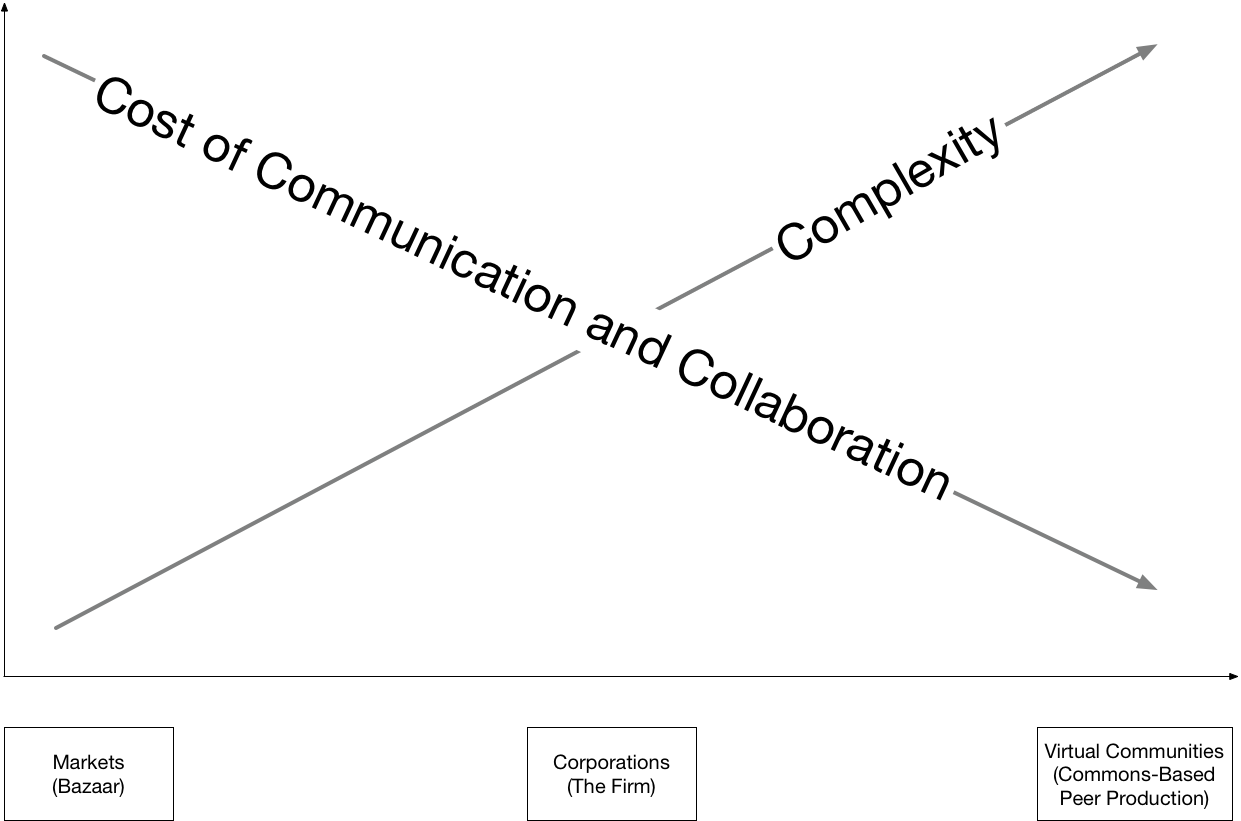
\includegraphics[width=1\textwidth]{pictures/TheInternetMarkets}
 \caption[The Internet decreased collaboration and communication costs and increased complexity.]{The Internet and communications technology have significantly decreased the cost of collaboration and communication and increased complexity. Before the industrial revolution, most production occurred in markets. With the industrial revolution came corporations that increased efficiency through centralization of resources and management \cite{coase_nature_1937}. The Internet brought commons-based peer production - non-corporate production modes that allowed participants to assign their own labor with a more decentralized and bottom-up organization structure \cite{benkler_coases_2002}.}
 \label{fig:internetcomplex}
\end{figure}

Corporations continued to aggregate power, distribution, and capital, prompting a regulatory intervention in the United States ; the Sherman Antitrust Act was enacted to break up monopolies that were exerting complete control over the market \cite{ShermanA12:online}. The Internet, in many ways, led to even more decentralization and the creation of more competitive and dynamic markets where once monolithic telecommunications companies had dominated. However, twenty years in to the widespread rise of the Internet, companies such as Google and Facebook are now exhibiting monopoly-like scale and behavior. This new era of monopolies is built on digital networks rather than physical goods and distribution. (See figure \autoref{fig:netmonopoly}.)

\begin{figure}[t]
 \centering
 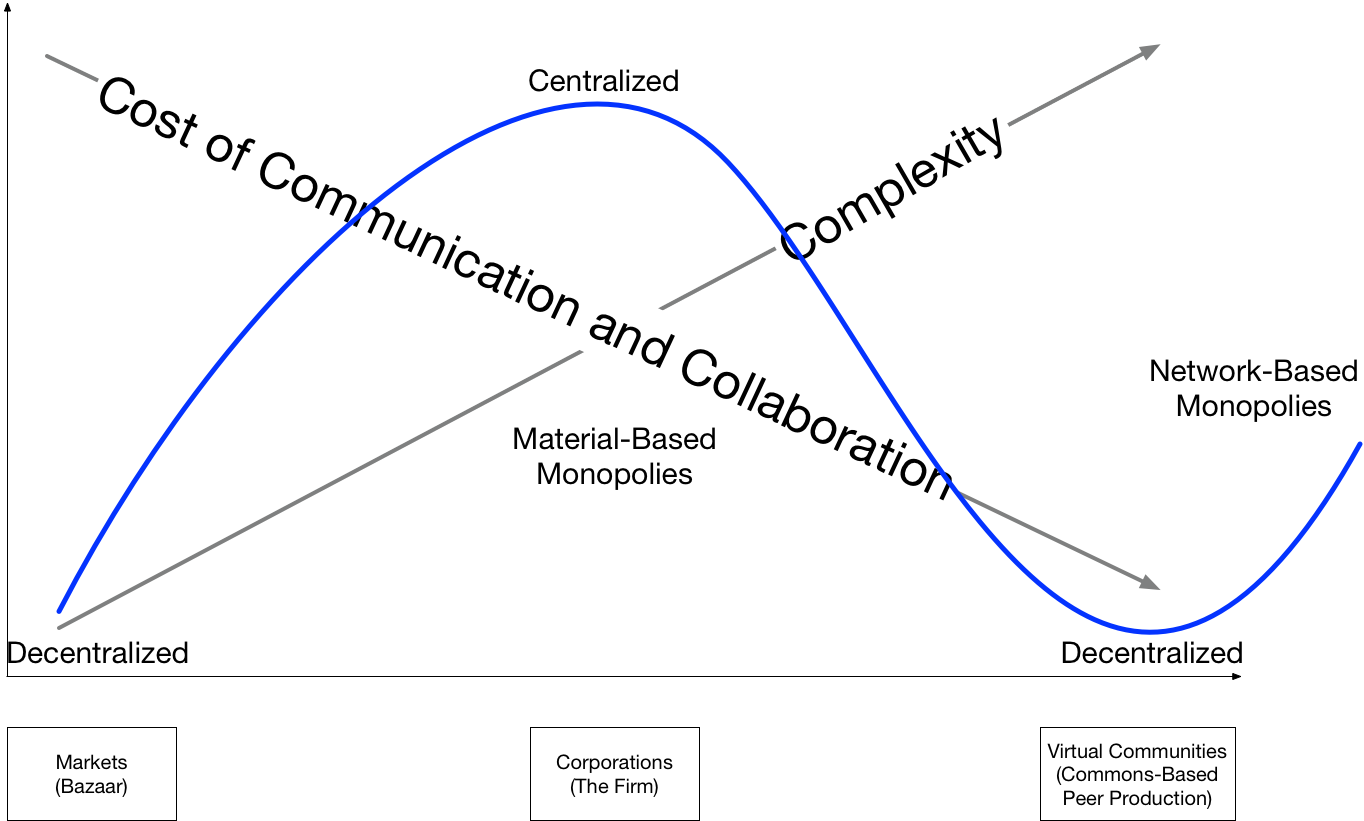
\includegraphics[width=1\textwidth]{pictures/TheInternetMarkets2}
 \caption[The Internet decentralized some monopolies but created new network-based monopolies.]{The Internet caused an unbundling of power and decentralization further diminishing the power of traditional monopolies such as telephone companies, but heralding a new generation of network-based monopolies in contrast to the material-based monopolies of the industrial revolution.}
 \label{fig:netmonopoly}
\end{figure}

The Internet has enabled organizations and movements to emerge in decentralized and bottom-up ways, but the nature of networks has also created a new kind of monopoly and centralization. These new monopoly-like enterprises have similar dynamics to the previous generation of monopolies. Our challenge is to use our new forms of organization and intervention to fight against these new forms of centralization as well as the old --- a post-Internet, community-based approach. We need to shift the paradigm of society from its orientation toward short-term capital to long-term flourishing, so that organizations and individuals can change their behavior, and the systems can evolve to become more robust and healthier.

In this dissertation, I describe the problems that must be addressed, present a theory of change, and explore concrete examples based on decades of practice. I present both a theoretical framework and practical approach for how we may transform society to address the complex problems we face today.

\section{Overview of Dissertation}
\label{intro:overview}

\begin{figure}[t]
 \centering
 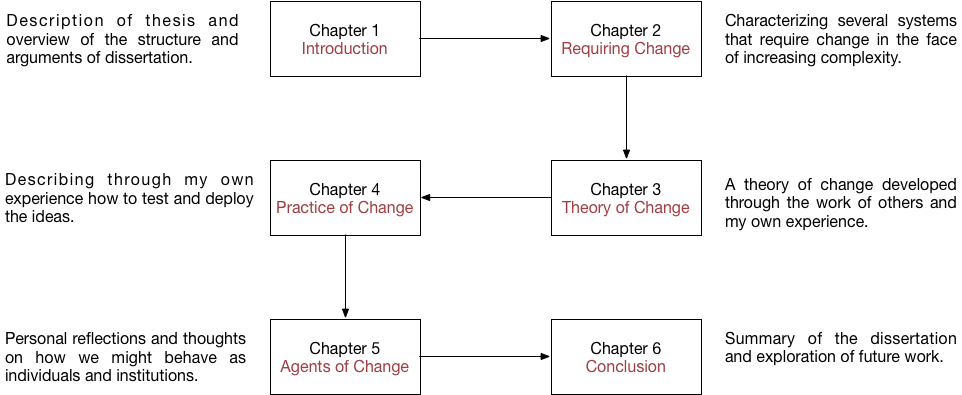
\includegraphics[width=1\textwidth]{pictures/thesisStructure2}
 \caption[Thesis Structure]{Thesis Structure: \textbf{\textit{Chapter~1}} describes the thesis and provides an overview of the structure and arguments of dissertation. \textbf{\textit{Chapter~2}} Characterizing several systems that require change in the face of increasing complexity. \textbf{\textit{Chapter~3}} presents theory of change developed through the work of others and my own experience. \textbf{\textit{Chapter~4}} includes personal reflections and thoughts on how we might behave as individuals and institutions. Finally, I end with a conclusion and an exploration of future work in \textbf{\textit{Chapter~5}}.}
 \label{fig:structure}
\end{figure}


The dissertation begins by describing five primary problem: the peril of silos; the problem of monolithic and centralized systems; the opportunity and need to rethink democracy in the post-Internet era; the need to rethink health and medicine; and how to address climate and environmental issues in \autoref{chap:requiring}.

In \autoref{chap:theory} I present a framework for understanding the systems we will be discussing. I draw on systems dynamics, evolutionary biology, cybernetics, design, history and philosophy of science, the history of the Internet, and lessons from Lawrence Lessig. I share my own thoughts on the nature of the Internet and the perils of reductionist thinking. I argue that the only way to change the system is through a paradigm shift in theories and methods of change. I argue that the intervention is best delivered through an artistic and cultural intervention, using the hippie movement as an example.

In \autoref{chap:practice} I describe how the Media Lab works, using several of the initiatives at the Media Lab as examples of an ``antidisciplinary'' approach to address the peril of silos. I then share my work as the CEO of Creative Commons, a board member of The Open Source Initiative, my work in the cryptocurrency communities since the 1990s, and my work in the venture and venture capital community to describe my learnings from, and contributions to, decentralized architectures. I share my work on various layers of the Internet infrastructure, including my role in the development of social media and the new public sphere, and my teaching and research in the ethics and governance of artificial intelligence. I consider these as contributions to reinventing the new post-Internet democracy. I discuss my course, ``Principles in Awareness'' at the Media Lab that I teach with the Venerable Tenzin Priyadarshi that explores self-awareness. I describe the Health 0.0 initiative --- a new intervention to think about the future of health and medicine, and whether we can apply learnings from the Internet and the antidisciplinary approach. I also describe my work as the board chair of PureTech Health --- a new kind of biomedical company. Lastly, I describe my work on the environment, describing the citizen radiation measurement organization Safecast as an example not only of environmental activism but as a new way of using post-Internet organizational principles to create grassroots activity. I also share the efforts of the Nia Tero organization to protect the environment through collaboration with indigenous people and local communities.

In \autoref{chap:agent} I reflect on my own journey and address some of the questions that were raised during the dissertation defense and in feedback from the committee. I discuss happiness, conviviality, interest-driven learning, and how we might as individuals and organizations apply the lessons developed through the course of this dissertation.

\autoref{chap:conclusion} is a conclusion in which I reflect on my work experience and examine my successes and failures in the form of learnings and insights. I discuss what questions remain, and conclude with a direction for my future work based on a theory of change: a fundamental, normative shift in society away from the pursuit of growth for growth's sake. I argue that this new sensibility should draw on historical trends, indigenous sensibilities, and new values emerging from the environment created by new technologies and understanding of science.
 % Chapter 1 - introduction

%\cleardoublepage
%\ctparttext{\textbf{Part II} is the body of the dissertation broken up into three chapters. The three chapters, Requiring Change, Theory of Change and Practice of Change describe what we need to change, how we change and examples of the applications of those methods in my work.} 
%\part{Body} % Second part of the thesis

\chapter{Requiring Change} % Chapter title
\label{chap:requiring} % For referencing the chapter elsewhere, use \autoref{ch:examples} 

In this chapter, I describe several systems that require interventions as a result of the increasing complexity of their environments.

\section{The Peril of Silos}
\label{sec:silos}

Academic disciplines are essential for the advancement of the sciences and the humanities.

Academic disciplines create rigor and discipline to help validate claims; to create a common language and framework; to share tools; and to build on the work of others in the same field to advance the field in effective ways. Academic journals, departments and conferences create vibrant communities that enable members of disciplines to collaborate and go deeper and deeper into a particular topic or domain.

Dividing academic and human endeavor into fields and disciplines, however, has a negative side-effect: it creates silos that make it difficult to work across, among, or beyond specific disciplines. Each discipline has its own frameworks and language, and even when they are saying similar things, it's often difficult to communicate effectively with people in other disciplines.

Siloing has multiple causes:

Peer review, which is important to ensure that claims are properly established and that the contributions that take up journals' limited space are in fact worthwhile, often reinforces depth over breadth. This ever increasing specialization often contributes to disciplines becoming more isolated and siloed. For example, In ``Looking Across and Looking Beyond the Knowledge Frontier: Intellectual Distance, Novelty, and Resource Allocation in Science,'' researchers describe a study that randomly assigned grant proposals to 2,130 evaluators. The study found that ``evaluators systematically give lower scores to research proposals that are closer to their own areas of expertise and to those that are highly novel'' \cite{boudreau2016looking}.

Also, scientific journals over time exhibit a tendency to evolve from publishing applied papers to papers that are more and more theoretical and abstract. In their paper ``The delineation of an interdisciplinary specialty in terms of a journal set'' researchers show that the interdisciplinary field of communications studies became increasingly self-referential as dedicated journals emerged \cite{leydesdorff2009delineation}.

\marginpar{Ed Boyden, a colleague at the Media Lab who runs the Synthetic Neurobiology group, often refers to the famous adage that the American philosopher, Abraham Kaplan, talks about as ``the principle of the drunkard's search'': \cite{kaplan2017conduct} drunks sometimes look for their lost keys under lampposts because that is where the light shines.}In addition, many departments often hire new academics and graduate students to advance existing departmental fields and disciplines, thus avoiding the risk of hiring people who might complicate peer review, tenure, or funding. In short, they are less adventurous.

Government funding tends to also be distributed along disciplinary lines, reinforcing the work done in existing disciplines and the silos around them.

The siloing that these various factors lead to can make disciplines more comfortable, but less creative. Ed Boyden, a colleague at the Media Lab who runs the Synthetic Neurobiology group, often refers to the famous adage that the American philosopher, Abraham Kaplan, talks about as ``the principle of the drunkard's search'': \cite{kaplan2017conduct} drunks sometimes look for their lost keys under lampposts because that is where the light shines. Boyden talks about the need to create flashlights --- metaphors for the tools he and his team are designing and building --- to facilitate a search for keys that have fallen in the dark areas between street lamps. It turns out that there are a lot of keys lying around in those dark spaces.

In fact, abundant evidence shows that the majority of useful inventions are discovered while looking for something else. A 2005 survey of European patents \cite{gambardella_value_2008} found that nearly half of the underlying inventions ``[arose] unexpectedly from research projects undertaken for other purposes or from activities other than inventing'' \cite{kennedy_opinion_2016}. \emph{The New York Times} reported on other studies with similar results.

Bridging disciplines is not a new idea. Interdisciplinary study has been widely and successfully pursued, generating new fields such as bioengineering, and unlocking tremendous value. New disciplines are often born at the intersection of old disciplines.

But as more and more cross-cutting fields such as computation emerge, we find that the the evolution of traditional disciplines may not be fast or flexible enough to deploy people and resources in the necessary fields to avoid being outpaced by technology, opportunities, and threats.

It is not only academia that is segmented and siloed. Corporations hit by the advances in the Internet have found themselves in completely new industries. For example, newspapers are competing with social networks, Craig's List, and mobile apps more than with other newspapers. Companies' IT strategies can no longer confine themselves to back rooms. Newspaper companies are having to learn about online video. Pharmaceutical companies are having to embrace artificial intelligence in the search for new drugs. At the same time, computer software companies are having to develop ethics policies.

\section{Monolithic and Centralized Systems}
\label{monoliths}

When Alexander Graham Bell invented the telephone, his business model was to lease out phones and hire contractors to run wires between them. The early telephone and telegraph companies strung wires from poles across the nation, controlling the entire network infrastructure, from local telegraph offices to the telephones. in people's parlors. This made sense when the technology was relatively simple, and controlling and managing the network centrally allowed it to evolve as the technology advanced.

When communications became digital, we entered a new age of communications infrastructure.

The digital age brought many advances in technology including better sound, and it also gave birth to encrypted phone calls and fax machines. Engineers working at Bell Laboratories soon realized that when they tried to make the quality of the sound better, they disrupted fax and other data services. David Isenberg, who was a Distinguished Member of Technical Staff at Bell Labs at the time, wrote the seminal paper, ``The Rise of the Stupid Network'' \cite{isenberg1997rise}, asserting that a network provider should not try to optimize its network for any particular purpose, but rather should diligently deliver the bits reliably from one end of the network to the other (creating an ``end-to-end'' network as it is sometimes called), and allow innovation to take place at the edges --- phone, fax and other services. They didn't take his advice, and not long after fired him.

\marginpar{Through government regulation, civil society, and technical advances and protocols designed by the technical community, the products and services were unbundled and broken up together with the layers of the Internet, allowing innovation and competition on each layer, greatly enhancing services to users, and lowering costs. A similar unbundling is now beginning in the financial services sector.}\dw{YY I think this is the only chapter with callouts. Remove them for consistency?}However, the regulators and the market began to ``unbundle'' the telecommunications system --- separating into layers what had once been offered as a bundle. This was the key to the success of the Internet. In Japan, for example, the Ministry of Posts and Telecommunications intervened to allow small Internet service providers to be licensed to provide Internet connectivity and forced deregulation to allow us to lease layer two connectivity from the telephone companies and sell IP services directly to consumers. Later, the Ministry went even further forcing telecommunications operators to lease dark fiber allowing me, for instance, to lease dark fiber and ``light up'' both ends with my own hardware and connect to the \ac{JPIX} directly by peering through the \ac{WIDE} network.

Other countries are still ``bundled.'' In the United Arab Emirates, for example, \ac{VoIP} is still banned by the nation's Telecommunications Regulatory Authority and all voice traffic is controlled by the local telecommunications companies. While the Internet architecture consists of technically unbundled layers, businesses continue to try to bundle the layers to exercise pricing and product power, but their arguments have much less technical validity than before the Internet.  Debates such as the current one over net neutrality in the United States are over the commercial bundling of layers.

Encryption created new issues, complicating, for instance, the ability of U.S. law enforcement authorities to order wiretaps. Many believed that encrypting communications would decrease surveillance because wiretaps would be harder, and for that reason the government fought to ban encryption., while many of us fought for end-to-end encryption. Once it became clear that the government would not win the debate, in 1994 it passed the \ac{CALEA} that funded the development of, and mandated the deployment of, digital wiretapping technologies at the telephone companies. This paved the way for wiretapping at the massive scale revealed by Edward Snowden two decades later. This was a very frustrating event for us, and a lesson that even in a decentralized, layered system, regulators can take their interventions to another layer to get what they want.

Through government regulation, civil society, and technical advances and protocols designed by the technical community, the products and services were unbundled and broken up, together with the layers of the Internet, allowing innovation and competition on each layer, greatly enhancing services to users, and lowering costs. (This argument is more fully described in \autoref{decentralization}.)

A similar unbundling is now beginning in the financial services sector. The United Kingdom through the second Payments Services Directive (PSD2) is compelling banks to open their data in a standardized format to allow others to create products and services on top of existing financial institutions \cite{cortet2016psd2}. The new directive, called Open Banking, came into force on January 13, 2018 \cite{manthorpe_what_nodate}. The Monetary Authority of Singapore is pushing for a similar Open Banking initiative \cite{banking_singapore_2017}.

Unbundling fundamentally changes the ability of new entrants to come into the marketplace of both ideas and businesses, increasing the number of competitors and the amount of competition. As the telecommunications layer based on this unbundled system became more successful, it began to affect the next layer on the ``stack'' --- the layer of media and and the public sphere that was originally built on top of the older monolithic communications technologies. (See \autoref{layertable} in \autoref{decentralization}.)

\section{Emergent Democracy}
\label{emergentdemo}

As unbundling and the Internet drove down the cost of communication, it allowed everyone to become a publisher and a contributor to the global dialog. This dramatically impacted the nature of media and the public sphere.

\marginpar{We believed that blogs would evolve into a social medium that would transform democracy and make the world a wonderful, new place.}In 2003, I wrote an essay with the active participation of my online community as weblogs, or blogs, began to flourish \cite{1Emergen42:online}. Ross Mayfield who participated in these conversations coined the phrase ``emergent democracy'' to described what we believed was a new form of democracy emerging from our new tools. We believed that blogs would evolve into a social medium that would transform democracy and make the world a wonderful, new place. 

What follows is the first part of the essay, in which I described emergent democracy. As you will see, It was prescient about some things and quite naive about others. It serves as a marker in time, reminding us of how transformative we hoped and believed the Internet's decentralized architecture would be. (I have excluded the remainder of the essay because it deals primarily with the specifics of the tools that we had available back in 2003.)

\textit{Essay except begins here.}

\begin{quote}
Proponents of the Internet have committed to and sought for a more intelligent Internet where new democratic methods could be enabled to help rectify the imbalance and inequalities of the world. Instead, the Internet today is a noisy environment with a great deal of power consolidation instead of the level democratic Internet many envisioned.

In 1993 Howard Rheingold wrote \cite{rheingold1993virtual},
\begin{quotation}
We temporarily have access to a tool that could bring conviviality and understanding into our lives and might help revitalize the public sphere. The same tool, improperly controlled and wielded, could become an instrument of tyranny. The vision of a citizen-designed, citizen-controlled worldwide communications network is a version of technological utopianism that could be called the vision of ``the electronic agora.'' In the original democracy, Athens, the agora was the marketplace, and more --- it was where citizens met to talk, gossip, argue, size each other up, find the weak spots in political ideas by debating about them. But another kind of vision could apply to the use of the Net in the wrong ways, a shadow vision of a less utopian kind of place --- the Panopticon.
\end{quotation}
\marginpar{``It is also possible that new technologies will empower terrorists or totalitarian regimes. These tools will have the ability to either enhance or deteriorate democracy and we must do what is possible to influence the development...''}

Since then he has been criticized as being naive about his views \cite{rheingold2001virtual}. This is because the tools and protocols of the Internet have not yet evolved enough to allow the emergence of Internet democracy to create a higher-level order. As these tools evolve we are on the verge of an awakening of the Internet. This awakening will facilitate a political model enabled by technology to support those basic attributes of democracy which have eroded as power has become concentrated within corporations and governments. It is possible that new technologies may enable a higher-level order, which in turn will enable a form of emergent democracy able to manage complex issues and support, change or replace our current representative democracy. It is also possible that new technologies will empower terrorists or totalitarian regimes. These tools will have the ability to either enhance or deteriorate democracy and we must do what is possible to influence the development of the tools for better democracy. This sentence also from 2003 sounds both prescient and naive.

\subsubsection{Democracy}

In the dictionary definition, democracy ``is government by the people in which the supreme power is vested in the people and exercised directly by them or by their elected agents under a free electoral system.'' In the words of Abraham Lincoln, democracy is a government ``of the people, by the people, and for the people'' \cite{lessig2002future}.

Rome and most democratic nations since then have chosen a republican form of representative democracy. Direct democracy does not scale and because the uneducated masses were considered unfit to rule directly, those who were more ``fit to lead'' were chosen to represent the masses. Representative democracy also allows leaders to specialize and focus in order to formulate opinions about the variety of complex issues, which need to be resolved where an uneducated and uninterested population could not be expected to directly understand all of the issues.

The failure of democracy to scale is also not complicated to understand. The founding fathers of this country, the ``egalitie, fraternitie and libertie'' of France and most other liberals that moved society toward freedom and liberty in the 1700's could not have been expected to visualize the growth of populations, radical evolution of science, vast increases of technology and incredible increases in mobility of information, money, goods, services and people. Nor could they know or visualize the topography of countries such as the United States, Canada and China, or continents such as Africa, Northern Europe, Russia or Latin America. They laid out such vast topography to the best of their ability on grids that bore no resemblance to the reality of the environment or to the huge increases in scale of population commerce and government. In the main, they did not foresee a need for the right to self-organize --- to adjust scale and degrees of separation as such increases occurred \cite{deehockjoiitoweb}.

As the issues facing government become larger and more complex, new tools are enabling citizens to self-organize more easily. It is possible that such tools will enable democracies to scale and become more adaptable.

A democracy is ideally governed by the majority and protects the rights of the minority. For a democracy to perform this properly it must support a competition of ideas, which requires critical debate, freedom of speech and the ability to criticize power without fear of retribution. In a true representative democracy the power must be distributed into multiple points of authority to enable checks and balances.

\subsubsection{Competition of ideas}

A competition of ideas is essential for a democracy to embrace the diversity of its citizens and protect the rights of the minority, while allowing the consensus of the majority to rule. The competition of ideas process has evolved with the advancement of technology.

For example, the printing press made it possible to provide more information to the masses and eventually provided the people a voice through journalism and the press. Arguably, this has been replaced by the voice of mass media operated by large corporations. As a result, there is less diversity and more internalization of the competition of ideas.

\subsubsection{Critical debate and freedom of speech}

The competition of ideas requires critical debate that is widely heard. Although we have many tools for managing such debate, increasingly there are barriers to our engaging in it at all.

\marginpar{In the increasingly sophisticated world of databases and systematic profiling of individuals, the protection of those citizens and whistleblowers willing to question power must be assured.}

\subsubsection{The Commons}

\begin{quotation}If nature has made any one thing less susceptible than all others of exclusive property, it is the action of the thinking power called an idea, which an individual may exclusively possess as long as he keeps it to himself; but the moment it is divulged, it forces itself into the possession of every one, and the receiver cannot dispossess himself of it. Its peculiar character, too, is that no one possesses the less, because every other possesses the whole of it. He who receives an idea from me, receives instruction himself without lessening mine; as he who lights his taper at mine, receives light without darkening me.

That ideas should freely spread from one to another over the globe, for the moral and mutual instruction of man, and improvement of his condition, seems to have been peculiarly and benevolently designed by nature, when she made them, like fire, expansible over all space, without lessening their density in any point, and like the air in which we breathe, move, and have our physical being, incapable of confinement or exclusive appropriation \cite{jefferson1813letter}.
--- Thomas Jefferson
\end{quotation}

As the notion of intellectual property continues to grow in scope, more and more of what was one part of common knowledge is becoming the property of corporations.

As the infrastructure for communication becomes more tuned to the protection of property than the free spreading of ideas, the capacity for critical debate is severely constrained.

Even though ideas are not subject to copyright, increasingly draconian copyright protection legislation limits the scope and meaning of fair use and even the flow of innovation, thereby having the same effect as if ideas were property owned and controlled by corporations. It includes the code inside of the computers and networks, which controls the transmission or reproduction of information.

\subsubsection{Privacy}

Democratic or otherwise, rarely, very rarely, does any concentration of power or wealth desire to see subjects well informed, truly educated, their privacy ensured or their discourse uninhibited. Those are the very things that power and wealth fear most. Old forms of government have every reason to operate in secret, while denying just that privilege to subjects. The people are to be minutely scrutinized while power is to be free of examination \cite{deehockjoiitoweb}.

In addition to the legal and technical ability to speak and engage in critical debate, citizens must be allowed to speak without fear of retribution. In the increasingly sophisticated world of databases and systematic profiling of individuals, the protection of those citizens and whistleblowers willing to question power must be assured. The powerful are increasingly able to threaten the weak, and this power must be countered by an increase in the ability of people to manage their identities, which are more and more defined by the profiles created by electronically collected information.

It is essential to understand the difference between privacy and transparency. When the powerful collect information to control the weak and hide behind secrecy, this is an invasion of privacy and is the basis of a surveillance-based method of security.

In one of the earliest critiques of the ID card proposal (January 1986) Professor Geoffrey de Q Walker, now dean of law at Queensland University, observed \cite{davies_privacy_nodate}:

\begin{quotation}One of the fundamental contrasts between free democratic societies and totalitarian systems is that the totalitarian government [or other totalitarian organization] relies on secrecy for the regime but high surveillance and disclosure for all other groups, whereas in the civic culture of liberal democracy, the position is approximately the reverse.\end{quotation}

Steve Mann presents the notion of sousveillance \cite{mann2002sousveillance} as a method for the public to monitor the establishment and provide a new level of transparency. This has been the role of the press, but with its strong orientation toward positive feedback, the media has tended to focus on less relevant issues, which get an inordinate amount of attention. One such example was the media's fascination with Gennifer Flowers and her claim that she had had an affair with President Clinton.

Weblogs and other forms of filtering coupled with many of the capture and transmission technologies discussed by Mann may provide a better method of capturing and filtering relevant information while suppressing irrelevant information where the privacy damage exceeds the value to the public.
An example of weblogs exceeding the ability of the mass media to identify relevant information is the case of Trent Lott. The national media covered briefly his racist comments during Strom Thurmond's 100th birthday party. After the national media had lost interest, the weblogs continued to find evidence of Lott's hateful past until the mass media once again took notice and covered the issue in more depth \cite{shachtman2002blogs}.

The balance between what is relevant and not relevant is exceedingly difficult and important and culturally biased. Mechanisms to check the filtering mechanism for corruption and imbalance are necessary. It will be a variety of checks and balances and the combination of a diversity of methods that may provide us with the balanced view.

\subsubsection{Polling and Direct Democracy}

Direct democracy - the government of the public by itself - has always been said to be impossible on a large scale because of the technical difficulty of such direct governance and the fact that the complexities of involved in running a large state requires a much deeper understanding of the issues, specialization, and a division of labor. Representative democracy, wherein elected representatives of the people are chosen through a voting mechanism, is considered by most to be the only possible way to manage a large democracy.
As the voting mechanism becomes more organized and the difficulty of participating in the critical debate increases, we find that elected representatives represent people who have the power to influence the voting mechanism and the public debate. These groups of people are often minorities who have more financial influence or the ability to mobilize a large number of motivated people through religious or ideological means. The extremists and corporate interests dominate many democracies, and the silent majority have very little input in the selection of representatives or the critical debate \cite{rebuildjoiito}.

A variety of groups have been successful in polling the silent majority and amplifying its opinions to provide support for moderate politicians on policy issues. One such group, Peaceworks, operates in Israel and Palestine through polling, by telephone and the Internet, the average citizens who are in favor of peace and amplifying their opinions by then publishing the results in reports and the mass media. This method of bypassing the traditional methods of influencing representatives is a form of direct democracy, which is becoming increasingly popular and important as technology makes such polling easier.

Generally, polling, as a form of direct democracy is very effective for issues which are relatively simple and about which the silent majority have an opinion that is under-represented. For more complex issues, such direct democracy is criticized as populist and irresponsible.

To address this issue, Professor James S. Fiskin has developed a method of polling called deliberative polling. Deliberative polling combines deliberation in small group discussions with scientific random sampling to increase the quality and depth of the understanding of the participants while maintaining a sampling that reflects the actual distribution of the population rather than the distribution of political power. Deliberative polling has been used successfully to poll people about relatively complex issues such as tax policies \cite{fishkin2000deliberative}.

It is possible that there is a method for citizens to self-organize to deliberate on and address complex issues as necessary and enhance our democracy without any one citizen being required to know and understand the whole. This is the essence of an emergence, and it is the way that ant colonies are able to ``think'' and our DNA is able to build the complex bodies that we have. If information technology could provide a mechanism for citizens in a democracy to participate in a way that allowed self-organization and emergent understanding, it is possible that a form of emergent democracy could address many of the complexity and scalability issues facing representative governments today.

In complex systems the role of the leader is not about determining the direction and controlling the followers, but about maintaining integrity, representing the will of the followers and influencing and communicating with peers and leaders above \cite{FuturePo61:online}. The leader becomes more of facilitator and a custodian of the process than a power figure, and is often the catalyst or manager of a critical debate or the representative of a group engaged in one \cite{Leadersh1:online}. The leader is often the messenger delivering the consensus of a community to another layer or group. Indeed, some leaders in a representative democracy act in this manner. And as leadership becomes necessary to manage the development of an opinion or idea about a complex issue, information technology could enable quick and ad hoc leader selection and representation of that opinion or idea in a larger debate. 
\end{quote}

\textit{End of essay excerpt.}


\subsubsection{Postscript to Emergent Democracy}

\textit{Thoughts from 2018} \\


\marginpar{What we imagined, but weren't able to build, were systems of leadership, institution building and collaboration --- or what to do after established institutions are overthrown.}Through our participation in and understanding blogs and early user-generated-content, we had predicted the rise of a new form of voice and collective action and the role of social media on politics and opinion.

This essay was written in 2003 before the Arab Spring that began in 2010 with the Tunisian Revolution, spreading to Libya, Egypt, Yemen, Syria and Bahrain. The success of the Arab Spring in overthrowing regimes was attributed in great part to the use of social media. The Arab Spring demonstrated that these emergent systems could help overthrow established institutions.

What we imagined, but weren't able to build, were systems of leadership, institution building and collaboration --- or what to do after established institutions are overthrown. While the Arab Spring was able to overthrow the dictatorships in Tunisia, Libya and Egypt, the activists were not well equipped to take over the operation of the government, and only Tunisia has resulted in a transition to a constitutional democracy \cite{ruthven2016understand}.

More recently, polarization, hate groups, and extremism on the Internet have been become exceedingly influential in the political sphere, many focused on attacking established power, institutions and the elite.

I believe that unlike the civil rights movement, which had developed an institutional structure and carefully constructed organizations to follow through with strategy and law-making, many of the online movements are still impulsive. For example, Martin Luther King Jr. met with Mahatma Gandhi to discuss nonviolent protest strategy \cite{reddick}. However, examples such as the TimesUp Movement and the Parkland students protesting gun violence show a much greater degree of organization, strategy and focus, clearly learning from the past and developing new techniques, while remaining decentralized organizations that lack clear leaders or leadership structures.

As the public sphere and democracy are being disrupted and reinvented, we face similar challenges --- an imperative --- in health.

\section{Rethinking Health and Medicine}
\label{requiringhealth}

Recent advances in systems biology, neuroscience, immunology, gut microbiology, and many other related fields reveal that the human health system is far more complex than we previously understood. The nervous system, the immune system and microbial systems within the body are all highly interconnected and complex --- and different for each person. We do not fully understand how these systems work, and much of our understanding is reductionist and inaccurate. Treatment paradigms are based on models that identify target problems in an effort to identify and develop molecules that can be deployed into a patient to intervene in his or her biological system to solve a problem. The model for research has essentially been a method akin to trial and error, and approval for use of new treatments in human beings has required a series of trials demanding a tremendous amount of time and money, as stipulated by government. \marginpar{Despite new developments and huge investments, the pharmaceutical, health care and insurance industry is losing billions of dollars on complex, unpredictable and a largely unsuccessful drug development, clinical trial and research ecosystem that is unable to keep up with the new challenges and opportunities.}Pharmaceutical drug development mostly conducted in an ecosystem dominated by large monolithic incumbents regulated by government agencies has remained relatively unchanged for the last 30 years. Early discovery experiments, performed in vitro or in cell culture assays, are followed by translational studies in various animal models and then by clinical trials. The process is further slowed by the fact that performance in one model system doesn't necessarily generalize to the others, so that molecules that seem promising in in vitro models often drop out as they move through the development chain.

Despite new developments and huge investments, the pharmaceutical, health care and insurance industry is losing billions of dollars on its complex, unpredictable and largely unsuccessful drug development procedures that are unable to keep up with the new challenges and opportunities as our new research and technology is revealing just how vastly complex organic life is:

\begin{enumerate}
\item Systems biology, network medicine and bioinformatics approaches have been predominantly used for analyses and interpretation of medical data but have limited applicability at scale \cite{devita2015death}. For example, Vincent DeVita in \textit{The Death of Cancer} argues that the combinatorial complexity of cancer treatments make it impossible to understand at scale.
\item Biomarker discovery, automation of research tasks, diagnoses of medical images, clinical data and several other areas would likely benefit significantly with integration of emerging technologies such as machine learning and \ac{AI} (See \autoref{fig:drugai}), gene editing and the ``-omics,': the emerging fields that include genomics, transcriptomics, epigenomics, proteomics, and metabolomics.
\item Phase 3 outcomes trials conducted by large biotech companies are among the most complex experiments performed in medicine. Around fifty percent of Phase 3 trials fail. In the U.S. Food and Drug Administration's recently published white paper, ``22 case studies where Phase 2 and Phase 3 trials had divergent results'' \cite{22CaseSt45:online}, a common theme is the difficulty of predicting clinical results across a wide patient base, even with the backing of solid data. 
\item The mechanism of action for many candidate drugs and biologics remains unknown. This knowledge is key to the design and discovery of effective therapeutics.
\item Clinical trials are expensive and lack learnings and predictions that could be gathered from past experimental successes and failures of candidate molecules, adverse events and \ac{$IC_{50}$}\footnote{$IC_{50}$ is the half maximal inhibitory concentration and is used to measure the potency of a substance in inhibiting a specific biological or biochemical function.} measurements.
\end{enumerate}


We are discovering how complex and interconnected every system inside of our body is as well as how much our health is connected to every system outside of our bodies. Health is, at a different scale, very similar to the geological ecosystem which is also a massively complex system of interconnected systems.

\begin{figure}[h]
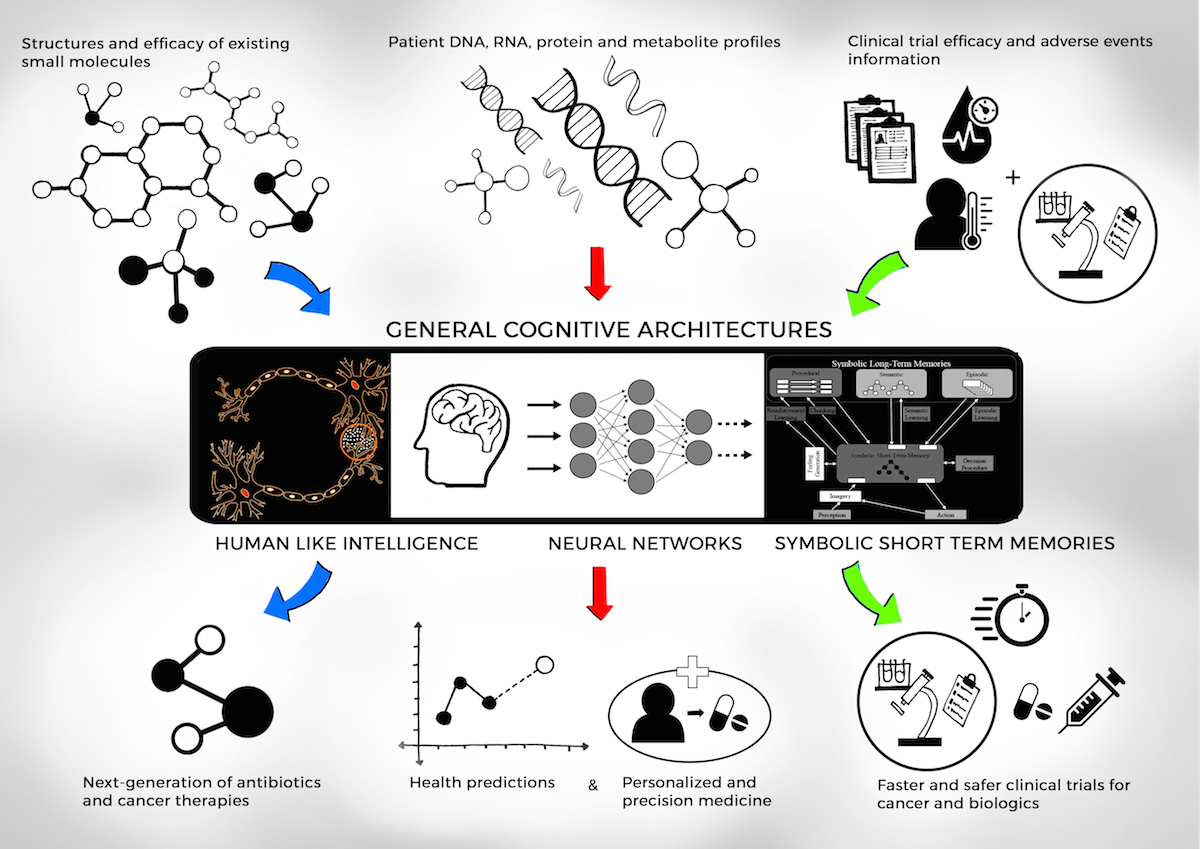
\includegraphics[width=\linewidth]{pictures/AI_DD-pratik}
\caption{Machine learning and artificial intelligence architectures for drug development. \cite{shahmlimage}}
\label{fig:drugai}
\end{figure}

\section{The Environment}
\label{sec:2environment}

In retrospect, it is clear that unbridled capitalism with a lack of feedback about what was happening to the environment has gotten us into the mess we call climate change. We had neither the measurements nor people properly positioned necessary for us to become aware of climate change and do something about it. \ac{NASA} even tried to stifle disclosure as the first climate scientists became aware of the issue \cite{winters2008investigative}. We now have a preponderance of evidence, but we are still at a loss as to how we're actually going to mitigate the worst effects of climate change, even as we watch them coming.

Most of our systems are designed to do things better and more efficiently without consideration for the costs and negative impacts that they are able to externalize, encouraged by the financial markets that reward the players who scale to create what consumers want to buy. These dynamics have led us to extract and consume so much of our natural resources with so little thought about the waste we are expelling back into the environment. 

We cannot expect the market to correct this on its own for it isn't set up to self-regulate or internalize these externalities. So I am currently working with my \ac{DCI} group and collaborators at the Emerson Collective on a way to account for ``natural capital',' adding to corporate balance sheets the value of the resources they use and the cost of the pollution they create. The aim is to make businesses put a price on their creation of what the British ecologist Garrett Hardin labeled ``The Tragedy of the Commons'' \cite{hardin1968tragedy}. We are exploring whether the blockchain or cryptography can help with the accounting of these types of assets and liabilities.

One concrete example is the use of carbon credits to create quotas on how much carbon companies put into the atmosphere, and allowing them to trade these credits to buy and sell savings in carbon emissions. The plan is to make a market for carbon emissions and other natural assets and liabilities that will help slow the exploitation of the natural systems. However, this is dealing mostly with ``stocks'' and some ``flows,'' to use words from systems dynamics.

Climate is, however, a highly complex system, and we are only measuring those elements that we know to monitor. James Hansen, an atmospheric physicists at the \ac{NASA} in the 1980s showed that key factors such as CO\textsubscript{2} and green house gases contribute to global warming \cite{hansen1981climate}, connecting fossil fuel emissions to climate change. My concern is that while greenhouse gases are clearly significant, it is easy to focus on only the most obvious and measurable elements of complex systems. We may be too focused on the atmosphere or on specific measurable parameters. 

Also, optimizing for any one variable can have unpredictable consequences in the long run. For example, biofuels which have been touted as an environmentally friendly alternative to fossil fuels, might have an opposite effort. Scientists argue that the production of ethanol from corn requires more fossil fuel energy \cite{patzek2004thermodynamics} the ethanol's energy value. In addition, the farming and processing methods are damaging the soil and causing other environmental side effects such as N\textsubscript{2}O release \cite{crutzen2007n}.

We need to adopt a systems approach to climate change. It is possible, if not likely, that the fundamental change that we need is a cultural intervention to redirect the sensibilities and behavior of consumers so that they spend money on products created with little negative impact on the environment...or, better, products created in ways that increase the sustainability of the planet.

Economists often say, ``\textit{when} the people in China and India are consuming as much energy and generating as much carbon per capita as Americans…'' rather than ``\textit{if} the people in China and India are consuming as much energy and generating as much carbon…'' Changing the norms of society may have more effect on the overall outcome than any accounting or policy change. Maybe we should promote a ``natural dream'' instead of the American Dream. 

It is also possible to change norms through policy interventions. Cars like the Toyota Prius and the Tesla are succeeding in part because of government subsidies to buyers and manufacturers. The success of these cars appear to be having an impact on norms.

Climate change is a complex global problem that is also local. Every town and village has a different context: ts energy requirements, its social dynamics, its industries and their impact on the local environment. Yet the architecture of markets and legal systems are often at state, national or even global scales. Change at a local level requires a bottom-up approach that can be coordinated but not literally managed in the traditional top-down fashion.

We need a social movement.

We need a theory of change --- a theory of the activation of communities.  % Chapter 2 - requiring change
% Chapter 3

\chapter{Theory Of Change} % Chapter title
\label{chap:theory}

Our challenges are complex, extremely important and require paradigm shifts and social movements to transform established institutions. To be successful, we need to develop a theory of change that takes into consideration both the historical context that has created the institutions, challenges and problems, as well as considering new technologies such as the Internet, artificial intelligence, and the blockchain.

I use a methodology inspired by the formal methodology called ``The Theory of Change'' that was created by and for the field of regional development and philanthropy \cite{brest2010power}. This theory of change methodology establishes primary long-range goals, and identifies the outcomes necessary to achieve those goals \cite{theoryofchangeprim}. Interventions are programs or initiatives that connect outcomes and goals. In \autoref{fig:theorychange} I have mapped my theory of change.

\begin{figure}[h]
 \centering
 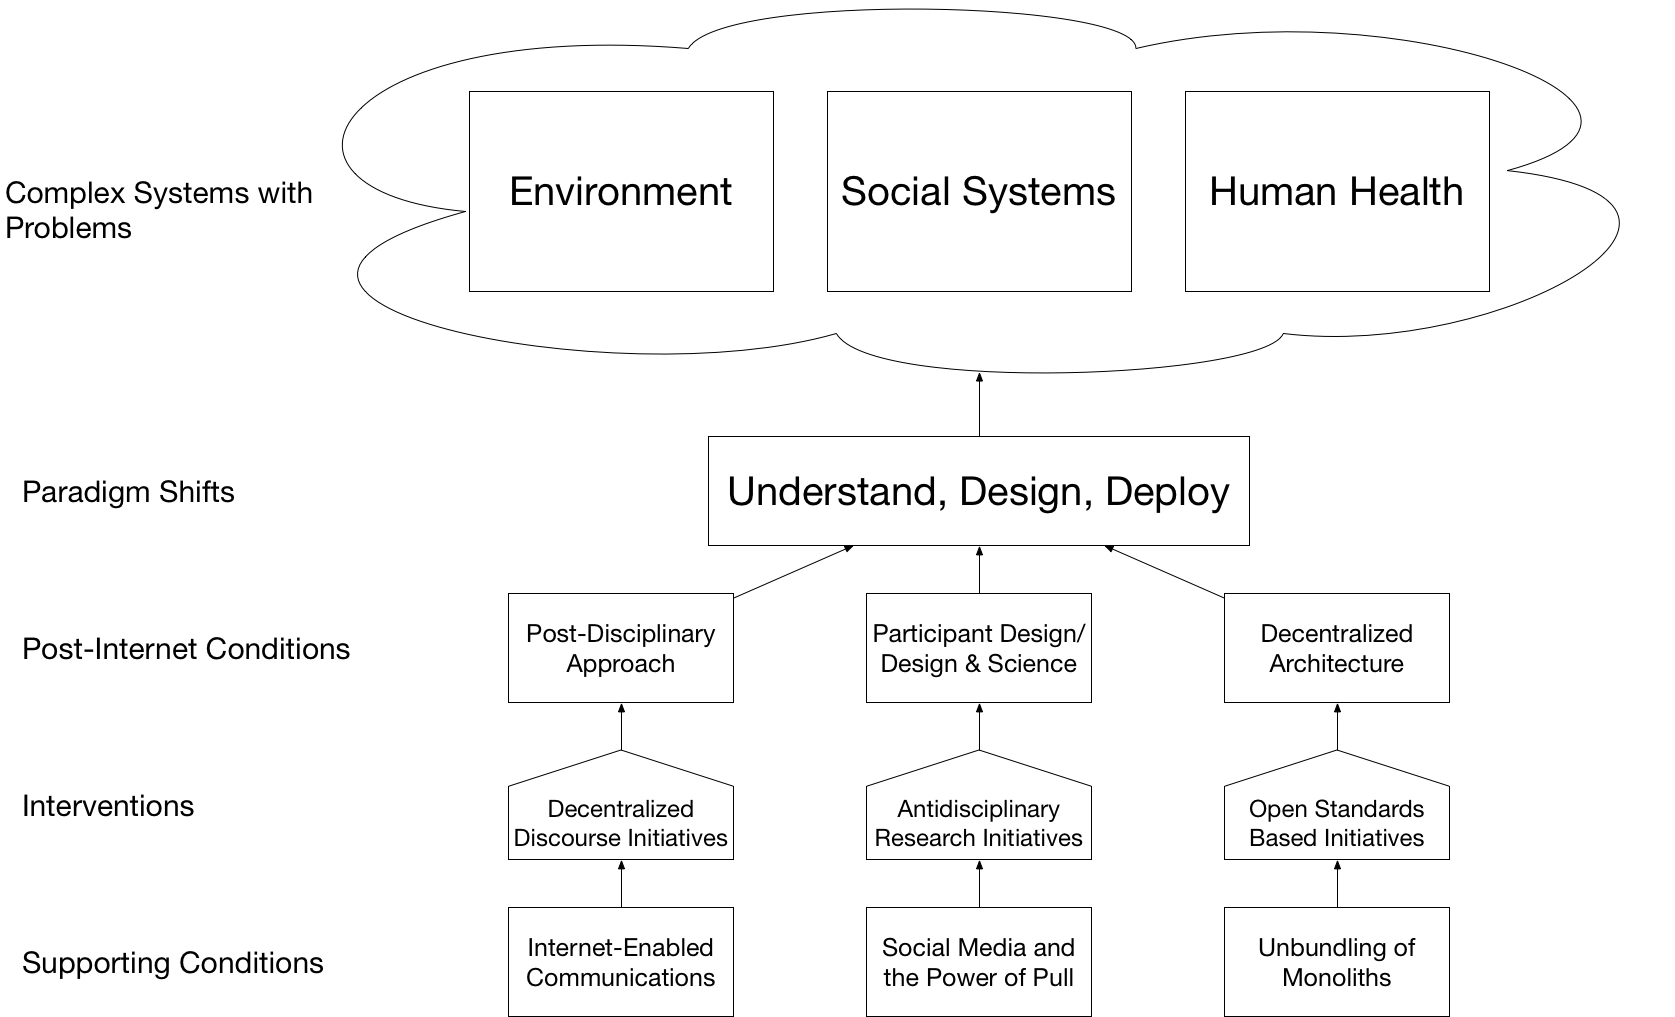
\includegraphics[width=1\textwidth]{pictures/TheoryOfChange}
 \caption[Diagram of my theory of change.]{My theory of change. In order to address the complex problems in the environment, social systems and human health, we must cause paradigm shifts to allow us to understand, design and deploy in complex systems. This paradigm shifts will require a post-disciplinary approach, a new participant design bringing together design and science and a decentralized approach with a decentralized architecture. These will require decentralized discourse initiatives, antidisciplinary research initiatives and open standards based initiatives. The Internet has caused new ways of communications, created social-media based organization models and provided a way for new open standards-based organization to break up traditional monolithic organizations.}
 \label{fig:theorychange}
\end{figure}

To address the problems in the environment, social systems and human health, we need a paradigm shift that allow us to understand, design and deploy interventions in complex systems. This paradigm shift will require a post-disciplinary approach; a new ``participant design'' process in which the participants in the system are the designers \cite{slavin_design_2016} (described more in \autoref{intro:design}); that brings together design and science; and a decentralized approach with a decentralized architecture. These in turn will require decentralized discourse initiatives, antidisciplinarity research initiatives, and open standards-based initiatives. We are ready for this paradigm shift because the Internet has created new forms of communications, social-media based organizational models, and the ability for new open standards-based organizations to break up traditional monolithic organizations.

I have long engaged in decentralized discourse initiatives --- that is, multi-way, open conversations that develop ideas and social relationships. As an early blogger (discussed in \autoref{sec:blogging}), I helped to bring blogs to Japan. Blogging inspired me to work on understanding emergent democracy (discussed in \autoref{sec:emergentdemo}). Some of my innovations in academic publishing include the \emph{Journal of Design and Science} and the MIT \ac{KFG} where we are experimenting with community and online-based publishing, challenging traditional academic publishing discussed in (\autoref{MITPress}). Also, the structure of the Media Lab that I am privileged to lead provides a decentralized, permission-free way to develop research and to carry on extended conversations about it (discussed in \autoref{antidisciplinaryapproach}).

Antidisciplinary research not only crosses disciplinary boundaries, but explores areas of research between and beyond disciplines that cannot be address by simple disciplinary intersectionality. For example, Health 0.0 reimagines diagnostics and therapeutics by fundamentally rethinking how we understand our biological systems, and by then developing and deploying technologies for treatment. This mirrors the way the Internet was developed by academics and grassroots communities outside of the incumbent industrial players (described in \autoref{sec:health00}). The Space Initiative is another example (described in \autoref{sec:spaceinitiative}). It takes advantage of the diminishing cost of space exploration and research to democratize participation in space exploration and research is. A third example is the Digital Currency Initiative at the Media Lab (described in \autoref{sec:DCI}). It aims at creating a core non-commercial, interdisciplinary, and antidisciplinary group to bring together and coordinate the development of standards and and technologies for digital currencies and the blockchain. It is situated in an academic environment, much like the early Internet was. Finally, the Ethics and Governance in Artificial Intelligence program --- the fund, course and research --- brings together all of the disciplines to forge a new interdisciplinary approach to thinking about and deploying artificial intelligence (described in \autoref{sec:EGAI}).

Examples of open standards-based initiatives include being the CEO of Creative Commons (described in \autoref{sec:CC}); being on the board of the Internet Corporation for Assigned Names and Numbers (ICANN); and being a board member of the Open Source Initiative described in \autoref{sec:OSI}. My commitment to open standards-based initiatives goes far back in my path. I helped set up and then served as the CEO of the first Internet service provider in Japan, PSINet Japan (described in \autoref{sec:PSI}). I co-founded Digital Garage, one of Japan's first web companies, which localized Infoseek Japan, one of the first search engines in Japan as well as providing other important Internet services. I advised and invested in in Havenco, an attempt to create an Internet hosting service outside of any government jurisdiction (described in \autoref{sec:havenco}). I have participated in the venture ecosystem first as an entrepreneur and later as an investor, with a primary interest in companies such as Flickr, Twitter and Kickstarter that have contributed to the Internet's open ecosystem.

\section{Understanding Change}
\subsection{Paradigms}
\label{intro:paradigms}

\marginpar{System dynamics and evolutionary dynamics can help us understand the dynamics of systems, as well as suggesting ways to intervene through a new design framework. One of the key insights of Meadows's work in systems dynamics is that the overall paradigms in a system drive the goals that then determine how elements in the system optimize. This view is consistent with evolutionary dynamics.}In his 1962 book, \textit{The Structure of Scientific revolutions}, Thomas Kuhn explains his idea of a ``paradigm'' by saying it is ``the set of common beliefs and agreements shared between scientists about how problems should be understood and addressed'' \cite{kuhn_structure_1970}. In a community or a social setting, paradigms can be the worldviews and values that silently shape thinking and research. From the perspective of systems dynamics, Donella Meadows says that the paradigm is that ``out of which the system --- its goals, power structure, rules, its culture --- arises.'' \cite{meadows_leverage}. Martin Nowak, director of the Program for Evolutionary Dynamics at Harvard, explains that in evolutionary dynamics and game theory, the paradigm determines the unit of payout for the game \cite{nowak2006evolutionary}. In a financial market system, for example, the payout is economic or financial gain. In biology, it is reproduction. Paradigms influence the fitness of strategies in evolution; the dynamics of communities; the behavior of complex adaptive systems, and what we can imagine and think. Paradigms can be transcended and altered, but there is no thinking outside of a paradigm.

System dynamics and evolutionary dynamics can help us understand the dynamics of systems, as well as suggesting ways to intervene through a new design framework. One of the key insights of Meadows's work in systems dynamics is that the overall paradigms in a system drive the goals that then determine how elements in the system optimize. This view is consistent with evolutionary dynamics.

\subsection{Systems Dynamics}

Climate change and disparities in health and income are highly complicated problems. Each is, in fact, a complex adaptive system, which means that its vitality and flourishing are not improved by working harder, doing more, or scaling. In the field of systems dynamics, which explores managing complex systems, the positive feedback systems that create exponential growth and that have the highest business payouts are typically viewed with alarm rather than envy because they tend to lead to unsustainable growth and ecosystem collapse.

\marginpar{Climate, health and income disparity are highly complicated problems. Each is, in fact, a complex adaptive system, and their vitality and flourishing are not improved by working harder, doing more or scaling.}The field of system dynamics was developed in the 1950s by Professor Jay Forrester of MIT. In 1972, the Club of Rome commissioned systems dynamics researchers to create a computer simulation of exponential growth in an environment of limited resources. The model used five variables, each growing exponentially: ``population, food production, industrialization, pollution, and consumption of nonrenewable natural resources.'' The report was called ``The Limits to Growth.'' Two scenarios showed ``overshoot and collapse'' in the 21st century, and one showed stabilization \cite{meadows_limits_2004}. Research continues in understanding resilience and the similarities between social systems and ecosystems \cite{folke2006resilience}. 

A simple system looks something like this (see \autoref{fig:meadows}).

\begin{figure}[h]
 \centering
 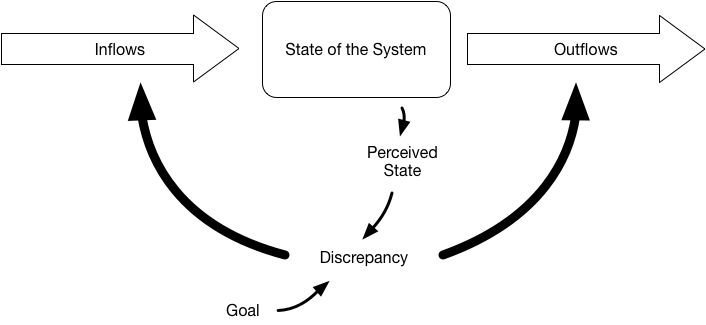
\includegraphics[width=1\textwidth]{pictures/System.png}
 \caption{Image of a simple system inspired by figure from Donella Meadows's essay \cite{meadows_leverage}}
 \label{fig:meadows}
\end{figure}

The state of the system, or the ``stock,'' is like the amount of money in an account, the amount of water in a lake, the amount of CO$_2$ in the atmosphere, or even the amount of trust in a government. Let's take the water in a bathtub as our example of stock. The inflows are the water flowing from the faucet. The outflows are water flowing out of the drain. By closing the drain and turning on the faucet, you can get the water, or stock, to increase in the tub. The ``goal'' is to get the right amount of water into the tub. You can watch the water level and control the inflow by turning on the water, or, if you end up with too much water after you sink into the tub, you could open the drain and lower the water level. It's apparent that it will be hard to control the water level of a tiny tub with a faucet connected to a fire hose, and that a large, overflowing tub of scalding water with a tiny drain will take a long time to cool.

Now imagine that you want to control the temperature. You might add hot water. But the boiler is far away in the basement,  so there is a delay after you turn the hot water knob. Then imagine the system that gets the water to your apartment and the system of energy behind the boiler. The energy might  come from a utility that provides you energy, but depletes your bank account. The goal of the utility is likely different than your goal when you are filling the tub for a nice warm bath: their goal may be to maximize their profits and take as much money from you as possible without depleting your bank account completely. The system gets complex quickly, especially since everything is interconnected...and the different systems may well have different goals.

See figure \autoref{fig:3sys} for an example of three systems connected together and \autoref{fig:9sys} for an example of nine systems connected together. Figure \autoref{fig:metasys} shows systems of systems connected together.


\begin{figure}[h]
 \centering
 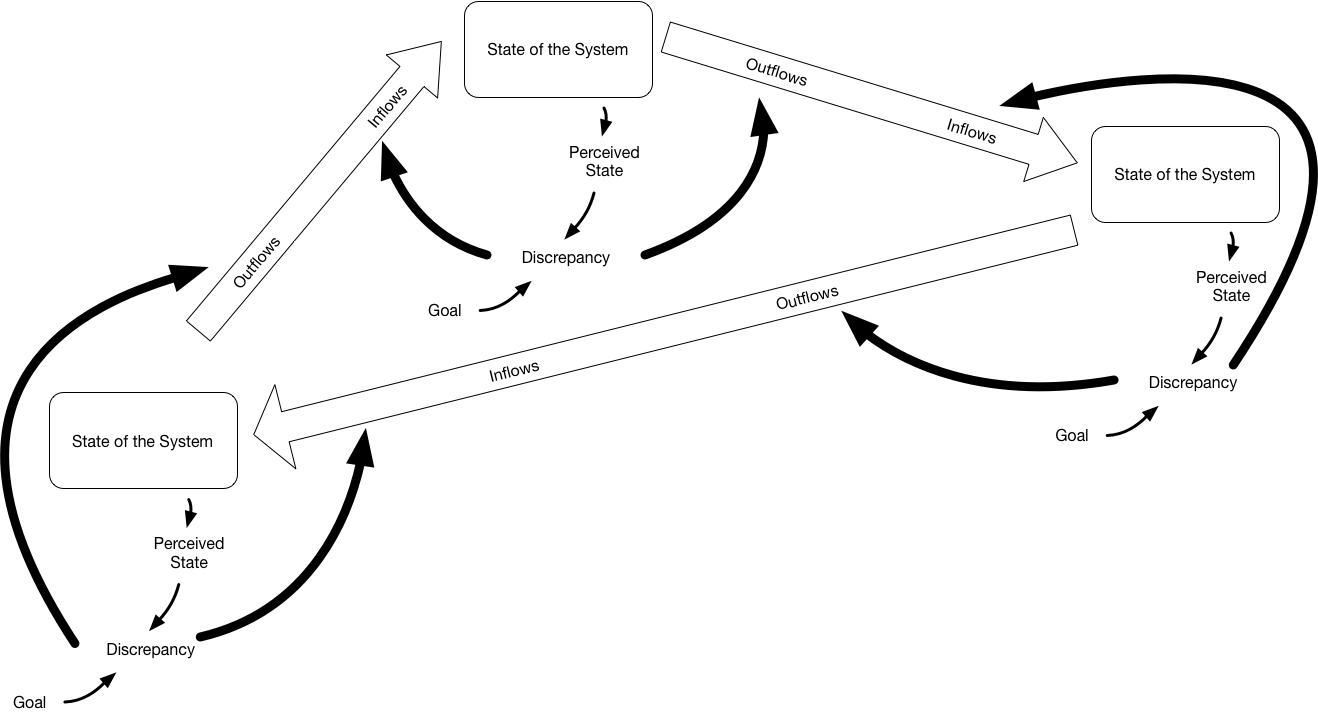
\includegraphics[width=1\textwidth]{pictures/3sys}
 \caption{Three systems connected together.}
 \label{fig:3sys}
\end{figure}

\begin{figure}[h]
 \centering
 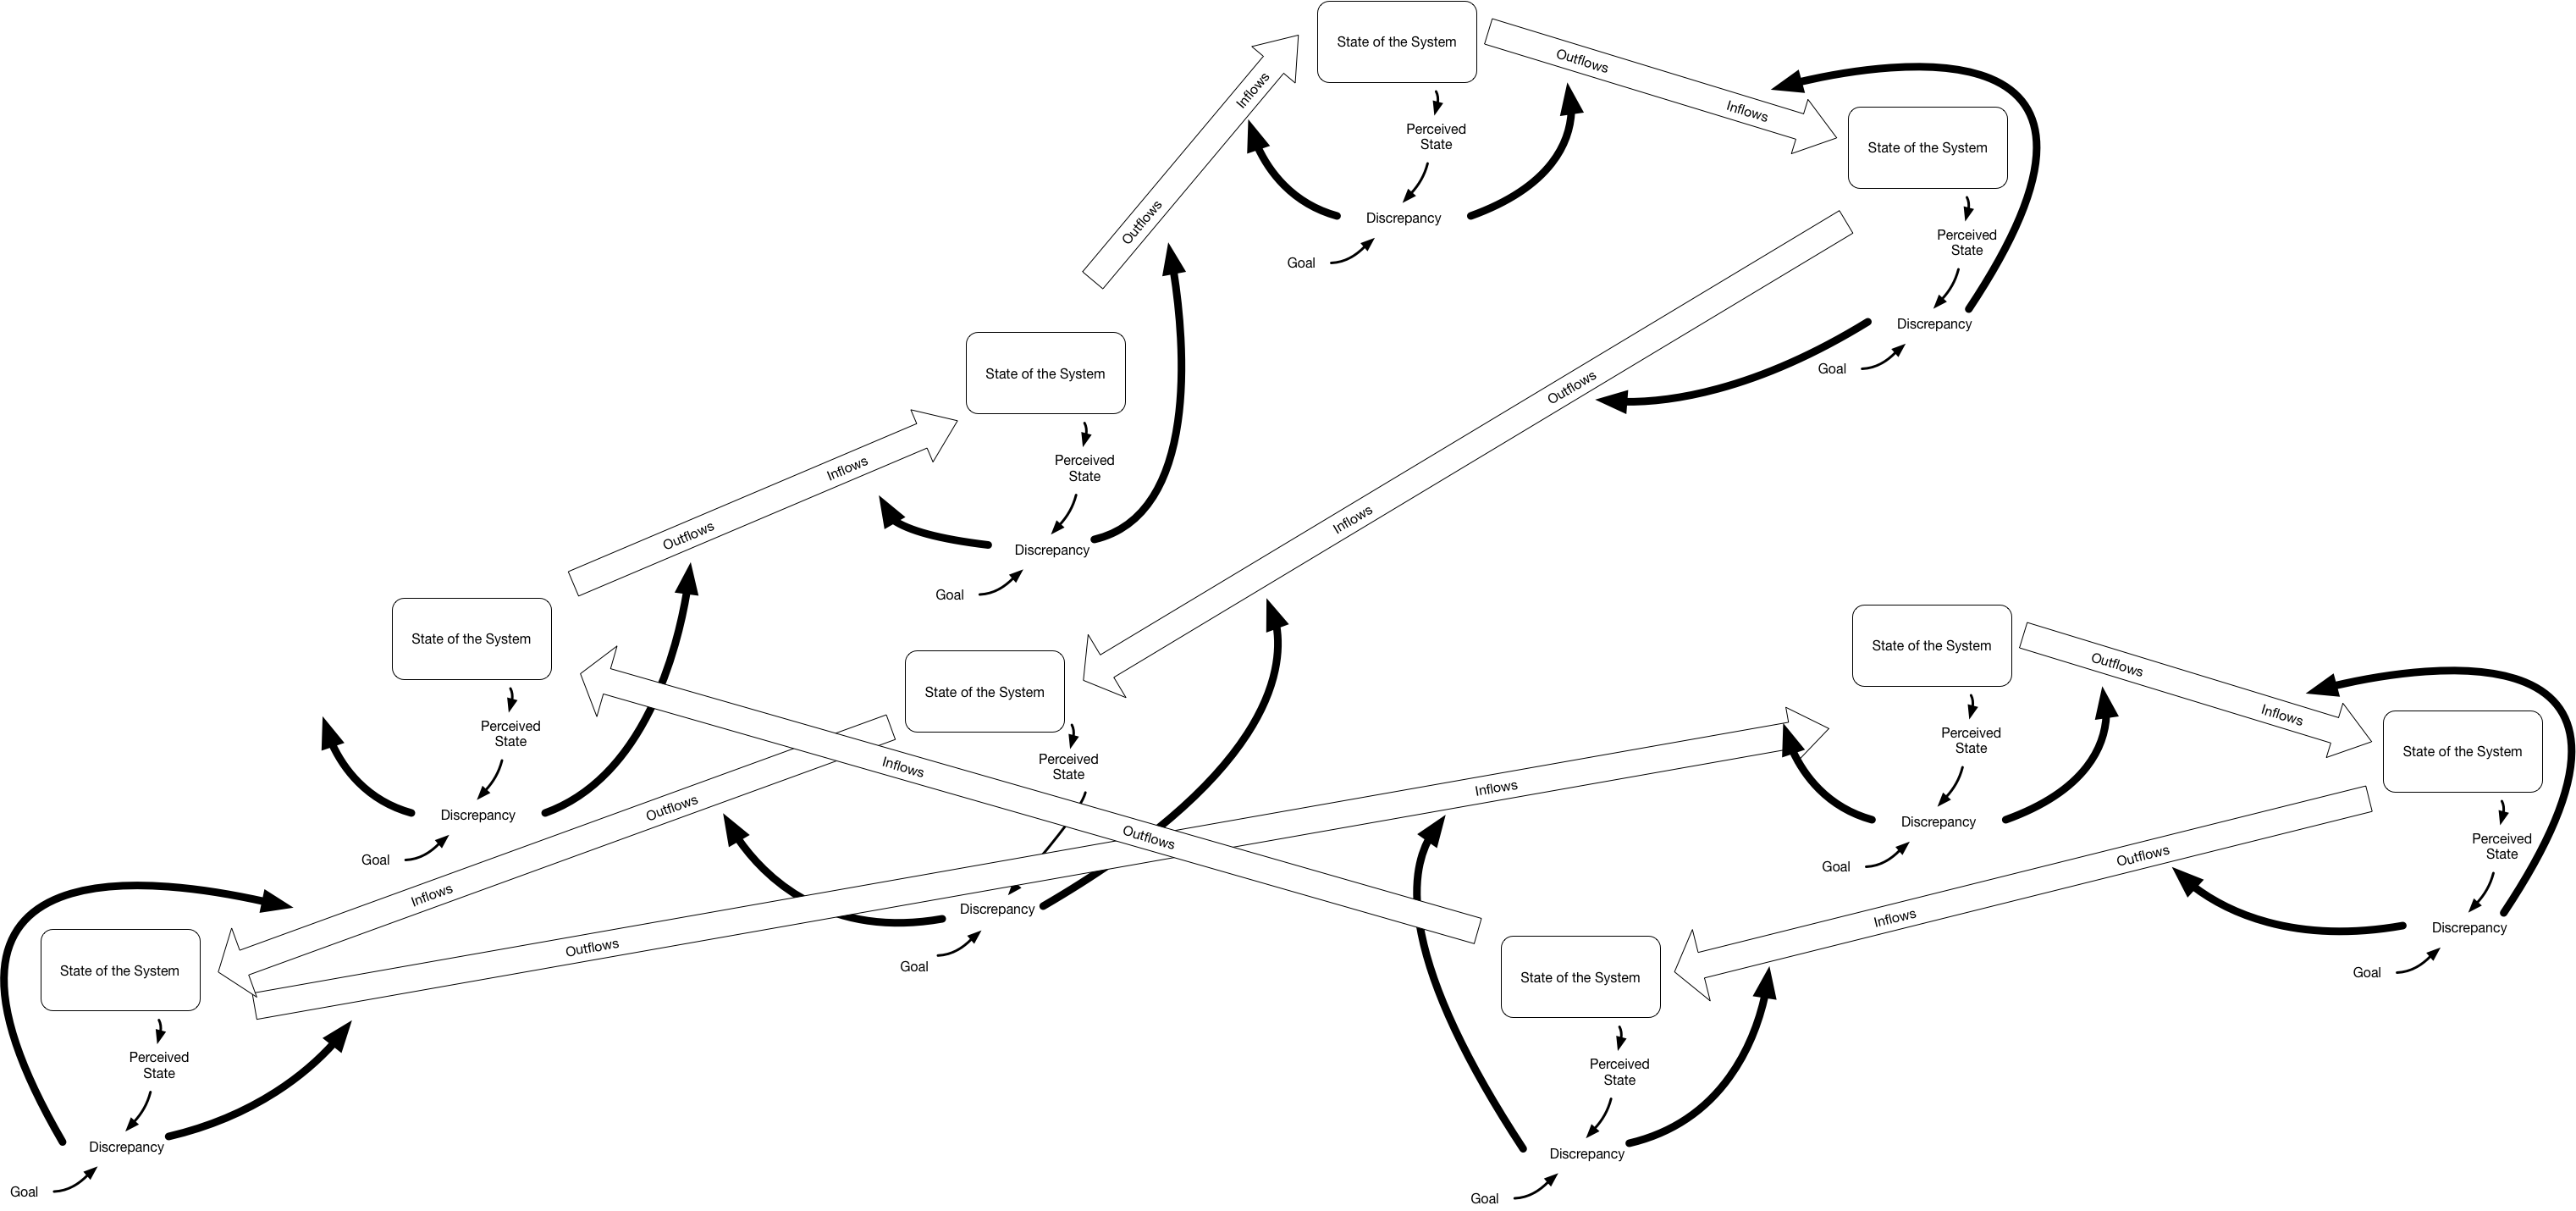
\includegraphics[width=1\textwidth]{pictures/9sys}
 \caption{Nine systems connected together.}
 \label{fig:9sys}
\end{figure}

A cell is a system with goals, and the human body is a system of cells with our own goals. Society is a system of individuals, communities, cultures, corporations etc. The planet is a system of societies, geological systems, other organisms, etc. Everything is a system of interconnected systems across scales.

\begin{figure}[h]
 \centering
 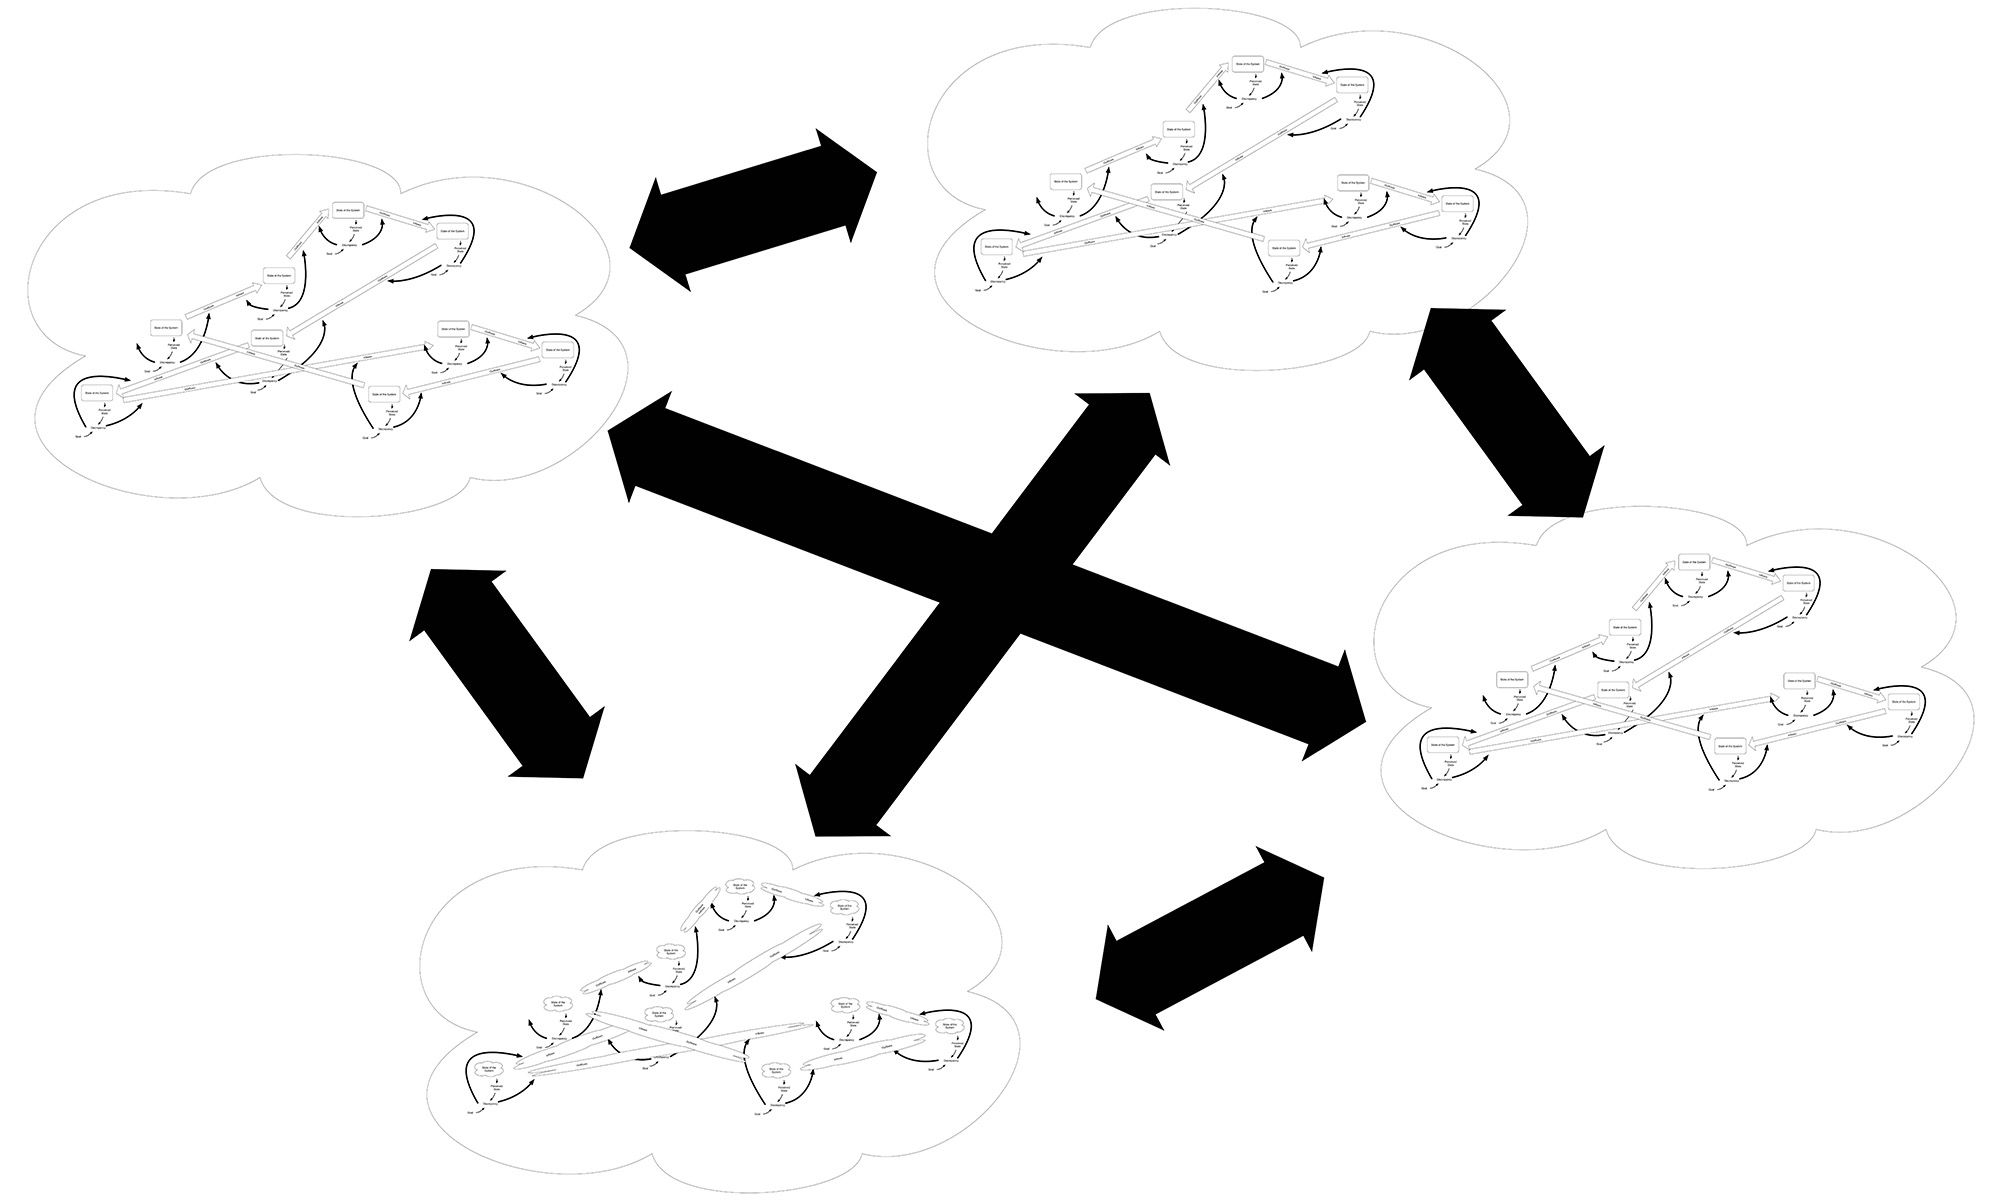
\includegraphics[width=1\textwidth]{pictures/metasys}
 \caption{A system of systems.}
 \label{fig:metasys}
\end{figure}

\subsection{Evolutionary Dynamics}
\label{intro:evolution}

\begin{figure}[h]
 \centering
 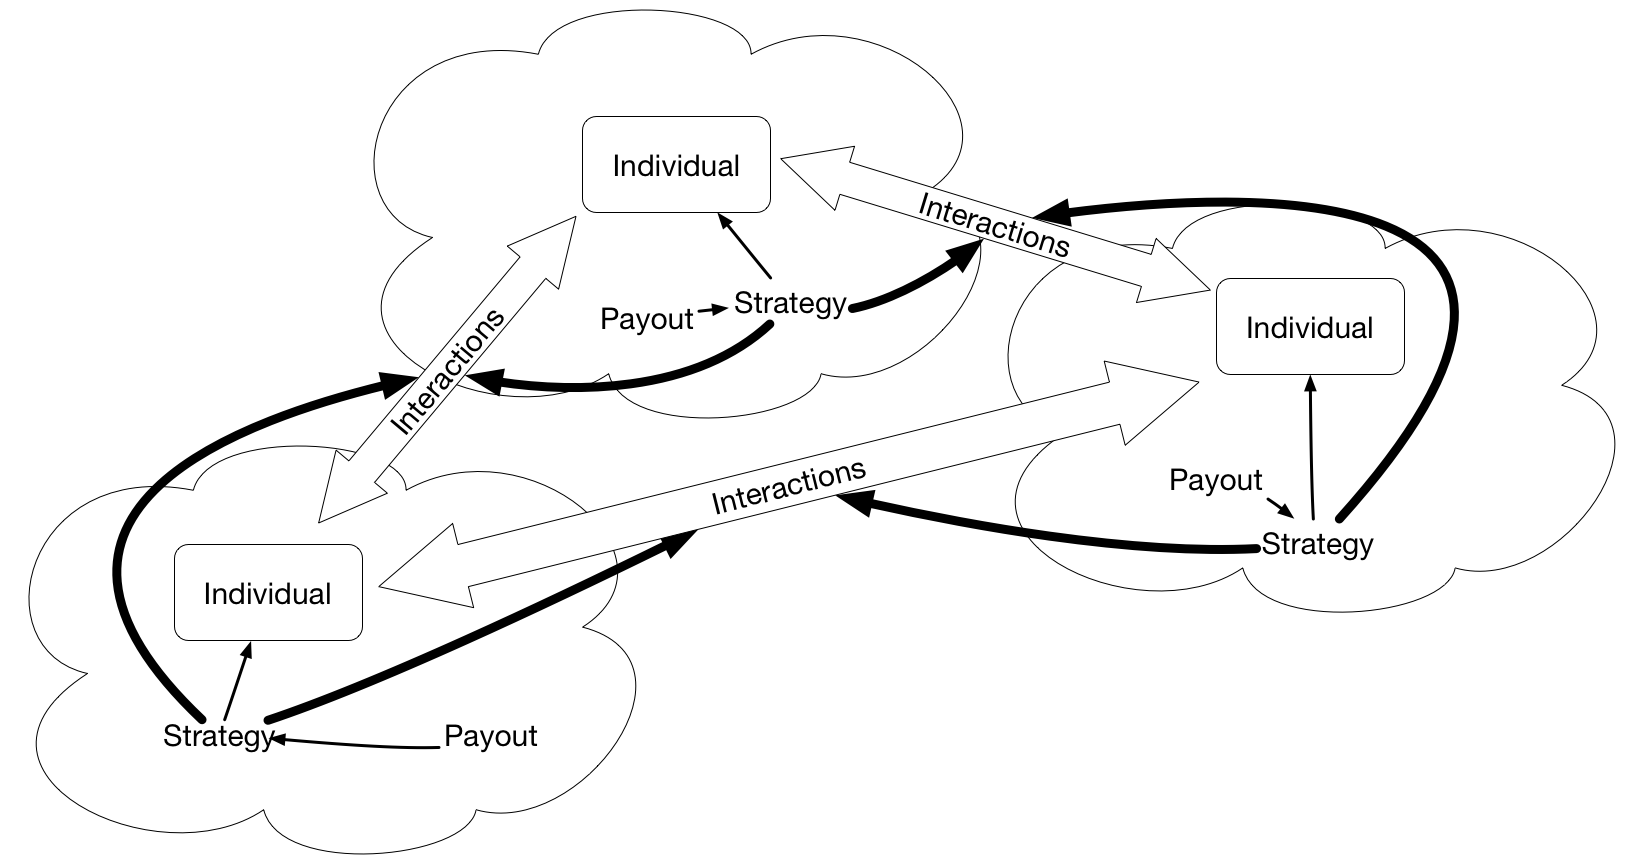
\includegraphics[width=1\textwidth]{pictures/EvolutionarySystem}
 \caption[Evolutionary dynamics version of interacting systems.]{Evolutionary systems look a lot like systems as described in systems dynamics, except that evolutionary dynamics does not use the term ``goals''. Instead individuals in a population interact with each other based on a strategy. This strategy optimizes for a payout from a ``game'' and the strategy evolves over time as the strategy of the other individuals change. \cite{nowak2006evolutionary}}
 \label{fig:evolution}
\end{figure}

While systems dynamics is useful in understanding the relationships between systems and how they behave, evolutionary dynamics is useful in understanding how systems evolve over time. (See figure \autoref{fig:evolution}.) Evolutionary dynamics is the evolutionary outcome of increasingly effective strategies individuals use to optimize for maximum payout \cite{nowak2006five, nowak2006evolutionary}. The payout is the measurement of the success and the fitness of a strategy; it is defined by the paradigm. Material value has been quantified by the emergence of money and the economy. The field of economics is able, through the utility function, to quantify in economic terms even immaterial payouts. While this is rational, humans have bounded rationality, and in practice, that has required traditional economic models to be reductionist.

The reducibility of norms into a utility function and economic motivation has been questioned by economists \cite{kreps1997intrinsic}. Workers who have internalized a company's welfare may get confused when extrinsic motivators in the form of economic incentives are implemented \cite{ichniowski1995effects}. Another experiment showed that people being paid to assemble Lego blocks would assemble more if the completed models were preserved rather than disassembled each time \cite{ariely2008man}. Individuals try to find meaning in even seemingly meaningless tasks, and are motivated in non-financial ways.

This evidence not withstanding, economists and business leaders continue to focus on financial extrinsic motivation as the key method for managing behavior. This necessarily reduces the diversity of strategies and decreases the robustness of our ecosystem. My argument is that the most difficult problems we face today --- climate change, global income disparity, and public health --- are a result of the effectiveness of solutions that maximized short-term payouts that we can measure and enjoy within our bounded rationality and perspective. Climate change can be directly linked to the success of industry in creating abundance at the expense of nature by exploiting and extracting resources. Much of modern chronic disease comes from agricultural gains that have made food abundant and cheap, and all manner of conveyance ensures we no longer need to walk and forage. The capital markets have become so efficient that passive capital continues to yield more and more returns, extracted from workers and society that are exceedingly underrepresented in setting strategy and participating in the payouts. There are, of course, ideas like the triple bottom line \cite{hall2011triple} and other attempts to nudge actors in markets to think longer term and behave more socially responsibly. While these attempts are an important move in the right direction, markets overall continue to optimize on shorter and shorter time scales, extracting more and more value from the future --- metaphorically very similar to the climate issue.


\subsection{Cybernetics}
\label{intro:cybernetics}

The Cold War era was defined by the rapid expansion of capitalism and consumerism, the beginning of the space race, and the dawning of the age of computation. It was a time when it was easier to believe that systems could be controlled from the outside and that many of the world's problems would be solved through science and engineering.

The cybernetics that Norbert Wiener and others described \cite{wiener1961cybernetics} during that period was concerned with feedback systems that can be controlled or regulated from an objective perspective. This so-called first-order cybernetics assumed that a scientist as an observer can understand what is going on, and therefore an engineer can design systems based on observations and insights from the scientist.

In the late 60s and early 70s, Margaret Mead, Heinz von Foerster, and others developed the notion of second-order cybernetics \cite{glanville2002second}: the cybernetics of cybernetics. Second-order cybernetics described adaptive complex systems, where the scientist-observer is part of the system itself.

While the study of systems dynamics and cybernetics continues, cybernetics reached an apex during a famous series of interdisciplinary meetings held between 1946 and 1953 as part of the Macy Conferences. The use of the word ``cybernetics'' in books peaked around 1969 (\autoref{fig:cybernetics}). Both cybernetics and systems dynamics flourished when they had heavy interdisciplinary participation and real impact. How disciplines and the communities that support them emerge and wither is a key topic of this dissertation, and the study of systems is a great example of numerous communities and approaches.

\begin{figure}[h]
 \centering
 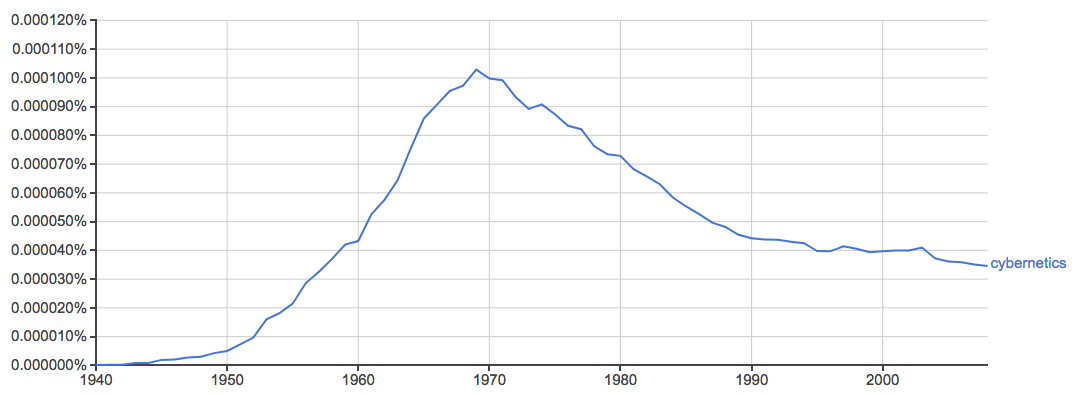
\includegraphics[width=1\textwidth]{pictures/cyberneticsuse}
 \caption[Graph of the use of the word ``cybernetics'' in books from 1940-2018 according to Google Books.]{Graph of the use of the word ``cybernetics'' in books from 1940-2018 according to Google Books. The word ``cybernetics'' increases in use rapidly after World War II peaking in 1969 with a steady decline for a few decades and leveling off.}
 \label{fig:cybernetics}
\end{figure}

We now have an opportunity and an imperative to pull the disciplines together again in the context of our new tools and our new challenges, and to tackle the wicked problems.

\subsection{Solving Complex Problems}

While systems dynamics and cybernetics have helped us model and understand complex problems, the really big and complex problems were described as ``wicked problems'' by Horst Rittel and Melvin M. Webber in ``Dilemmas in a General Theory of Planning.'' \cite{rittel_dilemmas_1973} They explain that these problems are beyond our ability to ``solve.'' ``Moreover, because of complex interdependencies, the effort to solve one aspect of a wicked problem may reveal or create other problems'' \cite{rittel_dilemmas_1973}.

Donella Meadows, a colleague of Jay Forrester at MIT who worked on the model for the Club of Rome previously described, proposed a way forward in her essay, ``Leverage Points'' \cite{meadows_leverage}. She suggests that since the goals of a system are generated by its paradigm, the ability to transcend the paradigm provided the most leverage for intervening in complex systems.

\section{Designing Change}
\subsection{Design}
\label{intro:design}

Most of what we design involves some part of a complex system such as the system that gets water into and out of a bathtub, but we usually just assume those support systems rather than focusing on them. For example, modern design is usually focused on the customer and the customer experience. For example, many ``Uber for food'' services like Doordash are a great experience for the customer. You have an app, you click it a few times to order food and before you know it, it's at your door. But what about the driver, the cook in the restaurant... what's the experience like for them? How much attention did the app developers give to their experience?

In the article ``Why I Quit Ordering From Uber-for-Food Start-Ups'' \cite{sloan2015quit} in \textit{The Atlantic Magazine}, Robin Sloan argued that the cooking/food service startup Josephine was better than food delivery services because it was designed for chefs as well as for customers. Josephine matched people who like to cook food in their homes with people in the neighborhood willing to pay to eat the food the home cooks made. This service was designed for the consumer \textit{and} the producer, and it also worked to promote a healthier neighborhood. The entrepreneurs behind Josephine looked at more of the system, not only the subject of the consumption. And that system is even more complex than Josephine recognized. It includes not only all humans in the neighborhood, but also the food supply chain, the food waste chain, and many other things that could be designed for as well.

\marginpar{In the \textit{Journal of Design and Science}'s first article, ``Design as Participation,'' \cite{slavin_design_2016} Kevin Slavin uses the quote ``you're not stuck in traffic, you are traffic.''}In the \textit{Journal of Design and Science}'s first article, ``Design as Participation,'' \cite{slavin_design_2016} Kevin Slavin uses the quote ``you're not stuck in traffic, you are traffic.'' Josephine was designed by people who understood home cooking aficionados and were closer to the system. But ultimately, if you really want to understand the system, you have to be part of the system. The design of a healthy complex system requires designers to be both observers of a system and humble participants in it.

At MIT, professors Neri Oxman and Meejin Kim teach a class called Design Across Scales. In this class, they describe systems at every scale, from the microbial and human to the architectural and urban to global and astronomical systems, and they demonstrate how all of these system are connected. Most scientists and designers are focused on a single scale and a single system, when instead they can and must understand how their work connects to and affects all systems at all scales and take responsibility for their interventions into these systems.

In ``Age of Entanglement,'' Oxman presents the Krebs Cycle of Creativity \cite{oxman_entanglement_2016}. This illustrates science adopting the perception of nature and converting it into knowledge. Engineering takes this knowledge and converts it into utility. Design takes this knowledge and converts it into meaning, behavior, and societal value. Art takes it and converts it into social perception. And although it's too rare, this should be in the input into science as well. My view is that science, engineering, design, and art need to work seamlessly together in order for creativity to be well expressed.

\begin{figure}[h]
\centering
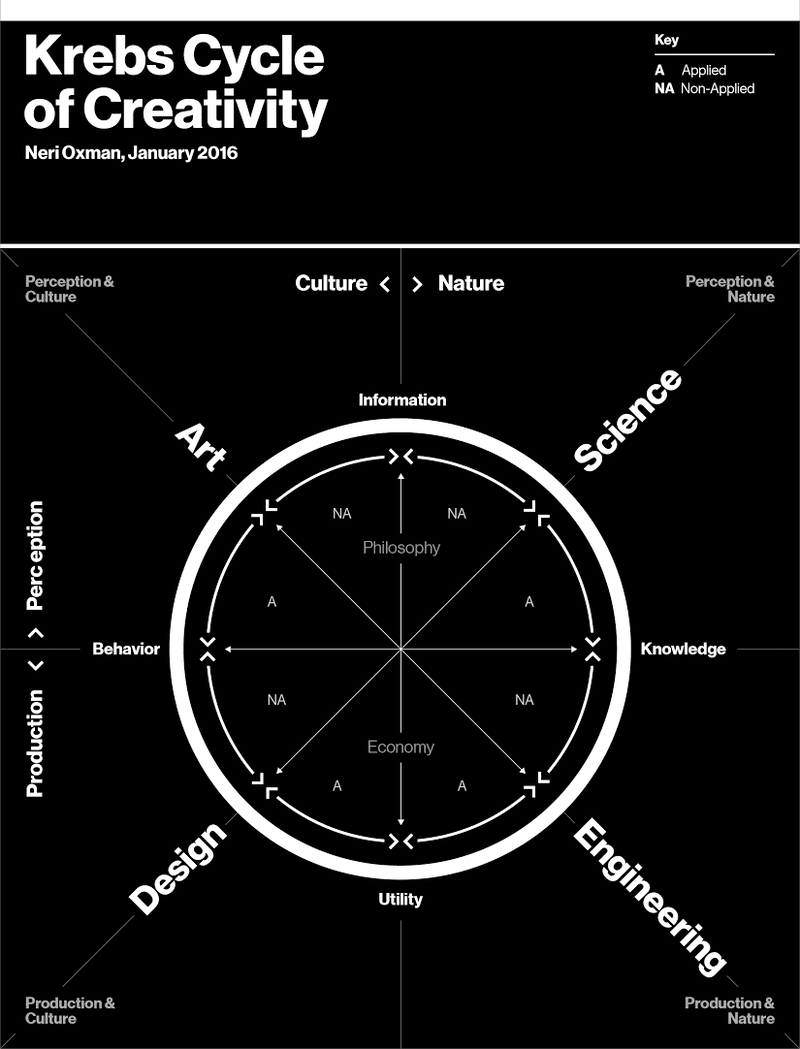
\includegraphics[width=.5\textwidth]{pictures/krebs.eps}
\caption{Krebs Cycle of Creativity \cite{oxman_entanglement_2016}}
\label{fig:krebs}
\end{figure}

In Oxman's Krebs Cycle of Creativity (\autoref{fig:krebs}), the relationship between the disciplines, design and science are opposite one another on the circle, and the output of one is not the input of the other as is often the case with engineering and design, or science and engineering. I believe that through the fusion of design and science, we can fundamentally advance both and provide ourselves with a new ``lens'' to view systems. This connection includes both the science of design and the design of science, as well as a dynamic relationship between these two activities.

I am using the term ``science'' to mean the study of biological and other hard sciences, whereas I mean ``design'' as a way to develop interventions in the environment and complex systems, in contrast to more tradition definitions of ``design science,'' which focuses on the methodological understanding of design as a process \cite{cross2001designerly}.

Much of design in the past was about the  visual and aesthetic. Modern design brought together form and function. In the 1896 paper ``The tall office building artistically considered,'' Chicago architect Louis Sullivan first proposed the notion of form following function \cite{sullivan1896tall}. Design and engineering came together to bring a social sensibility to the design of technologies from the mouse to user interfaces, from the physical to the immaterial. 

Today, many designers work for companies and governments, developing products and systems focused primarily on ensuring that society works efficiently. However, the scope of these efforts is not designed to include --- or care about --- needs beyond those of corporations or governments. We're moving into an era where the boundaries of various systems are not so defined. Systems such as the microbial system and the environment have suffered and now present significant challenges for designers. With such adaptive and complex systems, our unintended effects on them often produce unintended negative consequences for us.

\marginpar{Designers are not just planners wielding deterministic tools and control, but rather are participants in vast systems in which they exist and participate. This requires designers to employ a much more humble, non-deterministic approach and requires scientists and engineers to think across multiple scales and systems with greater intent and sensibility.}Designers are not just planners wielding deterministic tools and control, but rather are participants in vast systems in which they exist and participate. This requires designers to employ a much more humble, non-deterministic approach and requires scientists and engineers to think across multiple scales and systems with greater intent and sensibility. In ``Inviting Feedback'' in the \textit{Journal of Design and Science}, Pip Mothersill points out that, ``We don’t just design forms, we now design platforms'' \cite{mothersill_inviting_2018} and that those designing such platforms are designing ecologies.

Traditionally the domain of designers alone, this sensibility is a kind of aesthetic, though not merely a visual one. Rather, the field of design is trying to evolve beyond its traditional concern with visual aesthetics, and begin adopting a more philosophical aesthetic or sensibility, one more like that of indigenous peoples. The solution to the climate problem isn't more productivity, it is instilling a sensibility that ``more than enough is too much.'' Many of our contemporary health problems emerge from convenience, which is a modern commercial value that had no value at all in the rituals of the past. Income disparity is in many ways a function of a highly efficient capitalist system that rewards owners of resources, putting growth and progress above all else, and that exploits nature --- all concepts foreign, and even abhorrent, to many indigenous cultures, such as Polynesians and Native Americans, for example.

As we try to address problems like climate change or redesign systems like the criminal justice system, in the age of \ac{AI} such sensibilities and aesthetics are more important than compositional and structured tools like A/B testing or the economic models we currently rely on to shape our world. The linear and logical decision-making design that Herbert Simon describes in ``The Sciences of the Artificial'' \cite{herbert1978science} seems too reductionist for our complex problems. However, we must also be careful that our haste to resist reduction and structure does not lead to the ``structurelessness'' that resulted when the feminist movement rejected the idea of leaders, and thereby ended up with an informal and less accountable form of leadership, as described by Jo Freeman in ``The Tyranny of Structurelessness'' \cite{freeman1972tyranny}.

\marginpar{We must accept that the outcome of more and more scientific and technological design will not be fully in our control. It will instead be more like giving birth to a child and influencing its development. My work as director of the MIT Media Lab is to foster and nurture the use of respectful design in science and technology so that we enhance and advance the complex, adaptive systems we live within.}We must accept that the outcome of more and more scientific and technological design will not be fully in our control. It will instead be more like giving birth to a child and influencing its development. My work as director of the MIT Media Lab is to foster and nurture the use of respectful design in science and technology so that we enhance and advance the complex, adaptive systems we live within. 

\subsection{The End of the Artificial}

Unlike the past when distinct boundaries separated the artificial and the organic, the cultural and the natural --- science explored the natural and engineering built the artificial --- now it appears that nature and the artificial are merging.

Science and engineering today are delving into synthetic biology and artificial intelligence, which are both massively complex. These new areas of study and exploration necessarily take engineers out of the domain of the artificial and scientists into the domain of the natural. We are increasingly able to design and deploy directly into the domain of ``nature'' and in many ways ``design'' and ``edit'' nature. We have machine learning models that are exhibiting unpredictable and unexplainable behavior on the one hand. On the other hand, we are starting to see order in biology where we expect randomness. For example, while scientists argue that biology is inherently stochastic at the molecular level, research led by Deblina Sarkar has revealed nanoscale alignment of biomolecules in synapses between different neurons in brain that can not be explained without some coordinating and “ordering” mechanism, details of which are still unknown \cite{Sarkar2018}. We are therefore finding unexplainable order at the bio-nano-scale and unexplainable complexity at the digital-scale.

\subsection{Disciplines and Scholarship}
\label{intro:disciplines}

\marginpar{As we bring the artificial and the natural together and integrate the work of designers, artists, engineers, and scientists, the inability of academic disciplines to communicate with each other and our own difficulties conceiving ideas across disciplinary boundaries become significant impediments.}As we bring the artificial and the natural together and integrate the work of designers, artists, engineers, and scientists, the inability of academic disciplines to communicate with each other and our own difficulties conceiving ideas across disciplinary boundaries become significant impediments.

Linguistic relativists argues that language determines what one can think. This theory is controversial, but studies have shown that language does affect how we perceive color \cite{kay_paul_what_2009} or how we understand math \cite{everett_linguistic_2011, holden_life_2004}. If mathematics and mathematical symbols are a language, it is one that clearly limits or augments what we can imagine and discuss \cite{saxe_cultural_2012}. Michel Foucault, the French philosopher who pioneered modern thinking about the relationship between knowledge and institutional power, used the term ``épistémè'' to describe the space of possible, knowable things due to the rules and constraints of the language \cite{foucault_order_2002}. Foucault argued in \emph{Archeology of Knowledge} \cite{foucault_archaeology_2002} that knowledge is generated through discourse governed by the rules of institutions and the relationship between individuals. This is aligned with Kuhn's idea of paradigms as explained in\emph{The Structure of Scientific Revolutions} \cite{kuhn_structure_1970}: paradigms as linguistic formulations as well as codes of practice direct what and how knowledge is created and understood. \emph{Science in Action}. Before both Foucault and Kuhn, Ludwig Fleck, a Polish microbiologist and philosopher, had in the 1930s and 1940s described ``thought collectives'' as groups of people whose knowledge exists only because they are within the context and epistemology of that group \cite{fleck_entstehung_1979}.

Martin Nowak shows mathematically how learning from examples, or inductive inference, requires constraints \cite{nowak_computational_2002}. These constraints include the language constraints acquired by cultural evolution and the biological evolution of universal grammar \cite{chomsky_minimalist_1995}. In other words, you cannot learn anything through inference without constraints such as language. Indeed, Yuval Noah Harari, the Israeli historian argues in \textit{Sapiens} that ``the truly unique feature of our language is not its ability to transmit information about men and lions. Rather, it's the ability to transmit information about things that do not exist at all'' \cite{harari_sapiens:_2015}. So, we may need language even to conceive of that which is not there.

 \cite{latour_science_1987}, Bruno Latour, a French philosopher, argued that facts became facts through citation. Citations help form boundaries around disciplines, and simultaneously favors points of view that fit within the existing corpus, not ideas that question established theories and opens black boxes. Citations, according to Latour, serve a political purpose within disciplines. In ``Situated Knowledges: The Science Question in Feminism and the Privilege of Partial Perspective'' \cite{haraway_situated_1988}, Donna Haraway goes a step further, arguing that all knowledge is the result of ``power moves'', not moves towards truth. Disciplines under this analysis look like they are about power, not just knowledge.

So: academic disciplines are thought collectives with their own paradigms and specialized languages. Peer review reinforces adherence to those rules, paradigms, and patterns of language. The social dynamics that arise from the relationships among individuals in a discipline and the way funding and acknowledgement flow further reinforce the episteme, isolating disciplines from interaction with other disciplines. Disciplines package knowledge into bricks and black boxes \cite{latour_pandoras_1999} that may be used by other disciplines or subdisciplines without understanding the inside of the bricks themselves. Opening such black boxes and understanding what's inside is required for paradigm shifts and ``epistemological rupture'' \cite{bachelard_formation_2002} --- but that requires significant social and financial resources \cite{latour_science_1987}. Thus, the old adage, ``we are getting to know more and more about less and less'' \cite{fowler1911religious} is increasingly true. 

Approximately 2.5 million scientific papers are published each year \cite{jinha_article_2010}. In 2009, we passed the fifty million mark for the total number of science papers published since 1965. Fewer than one percent of scientists, however, publish a paper each year \cite{stokstad20141}. Just reading all the papers in a single discipline has become humanly impossible --- and publications represent only a small amount of the work in a field.

We clearly need to reconsider the way we develop knowledge and communicate within a discipline as well as between disciplines.

Interdisciplinary work has produced impactful results. Robert Langer, one of the most cited engineers in history \cite{noauthor_2610_2018}, helped bring engineering and biology together, creating the interdisciplinary field of bioengineering \cite{noauthor_struggles_2012, pearson_profile:_2009}. Multidisciplinary work has become much more common as computer science, engineering and other fields have converged to produce valuable results. However, these efforts suffer from lengthy and complicated beginnings; have difficulty finding funding; and require quite a bit of risk on the part of researchers who venture into research areas with no peers, no journals and often no obvious academic home.

\subsection{Rethinking the Disciplines}
\label{chap3:antidisciplinary}

\begin{figure}[h]
 \centering
 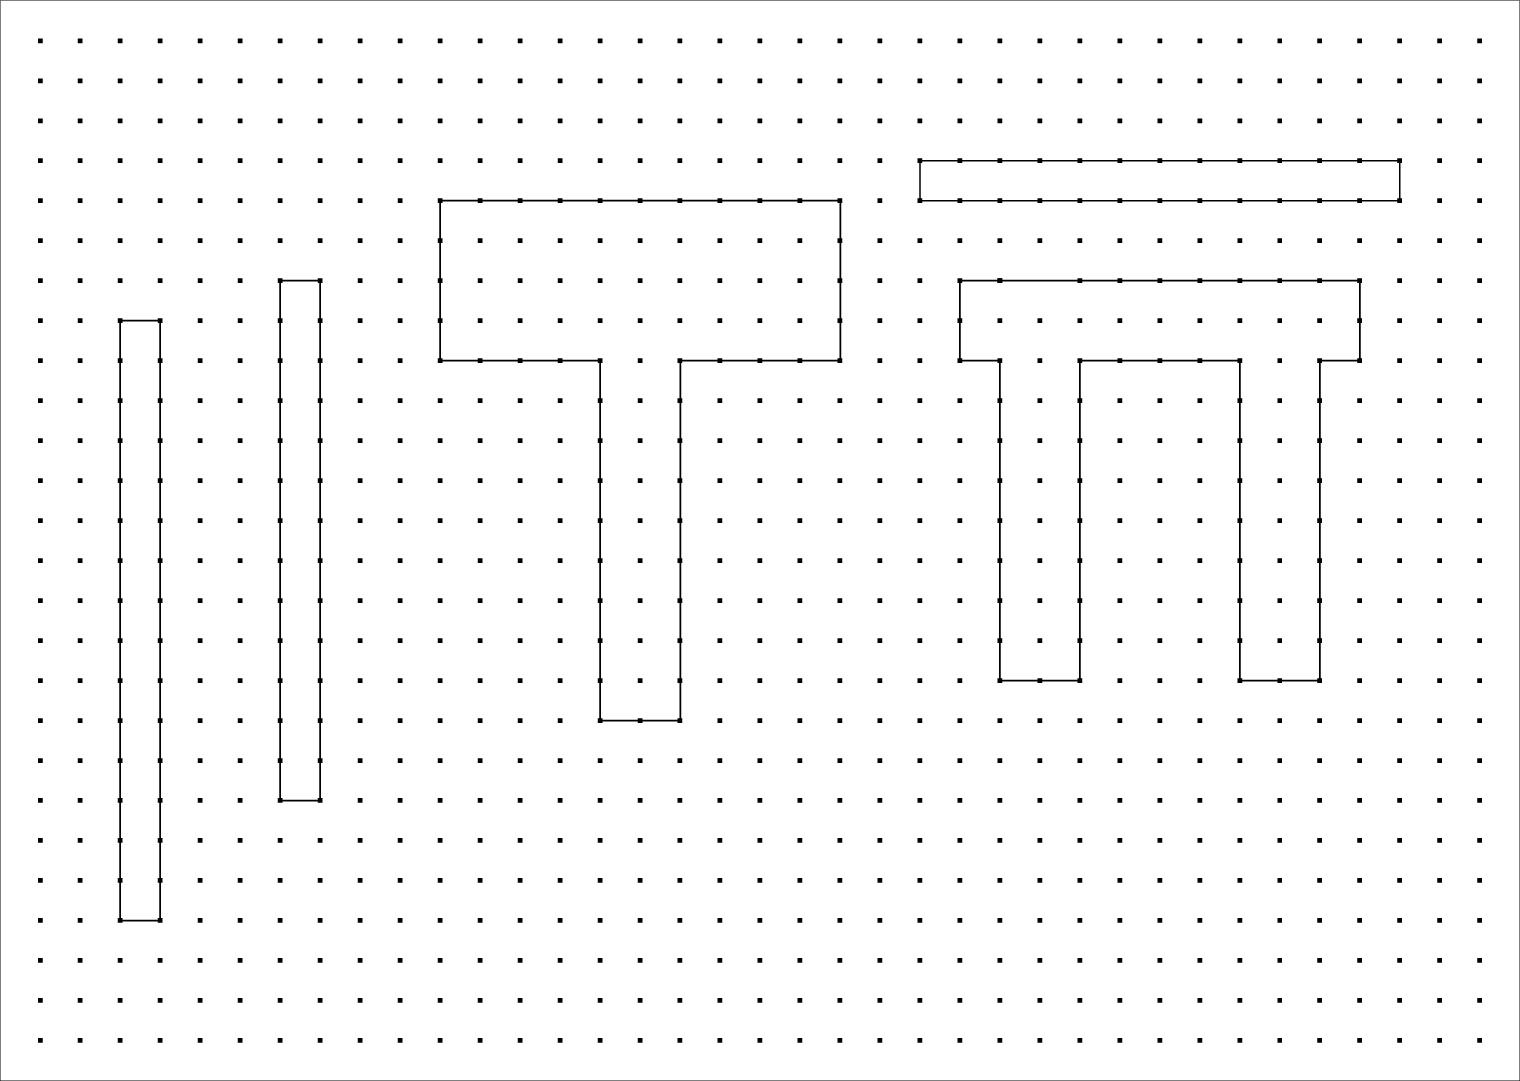
\includegraphics[width=1\textwidth]{pictures/JoiIllustr_V3-01.jpg}
 \caption[Image of shapes of disciplinary specialization.]{The vertical axis is depth. The horizontal axis is breadth. The horizontal line is normal non-academic people who follow the news. ``I'' people and specialists who go deep but can't explain what they do the the public. Some are specialists who can talk to the public but are sometimes less deep. ``T People'' are relatively deep but can talk broadly. Some people are ``$\pi$ People'' who are interdisciplinary.}
\label{fig:discipline001}
\end{figure}

\begin{figure}[h]
 \centering
 
\includegraphics[width=1\textwidth]{pictures/JoiIllustr_V3-02.jpg}
 \caption{``Multi-disciplinary people'' or ``M'' people are deep in more than two disciplines.}
 \label{fig:discipline002}
\end{figure}

\begin{figure}[h]
 \centering
 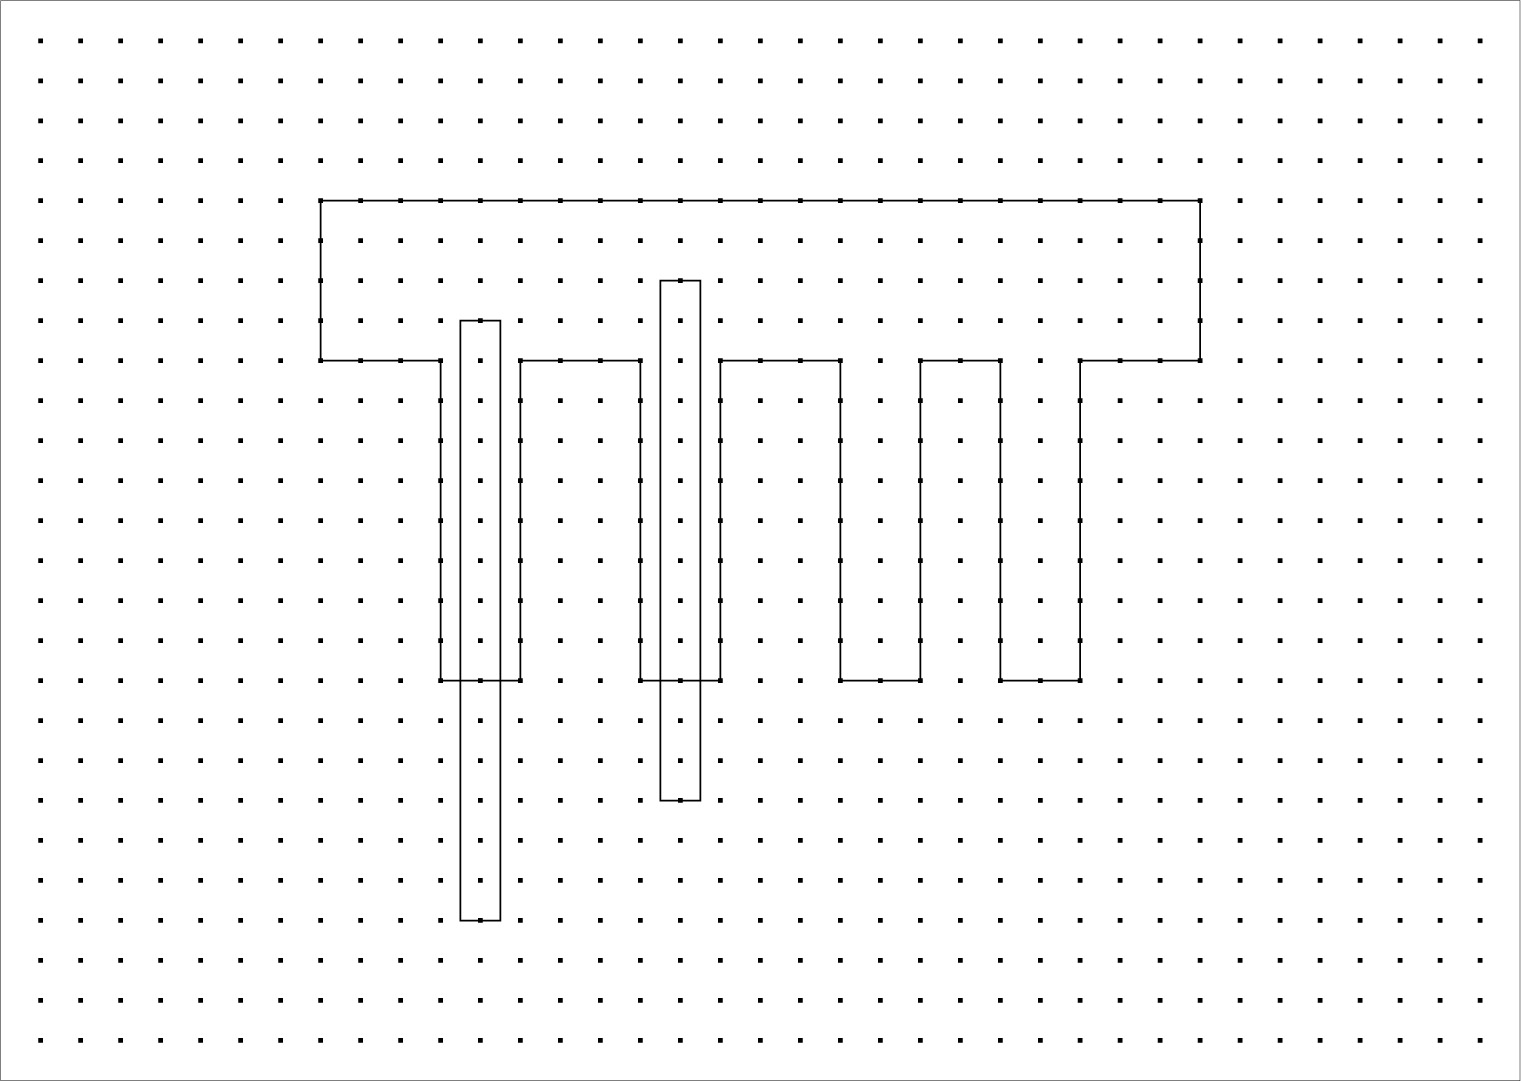
\includegraphics[width=1\textwidth]{pictures/JoiIllustr_V3-03.jpg}
 \caption{``M'' people can bridge people who are specialists in other disciplines.}
 \label{fig:discipline003}
\end{figure}

\begin{figure}[h]
 \centering
 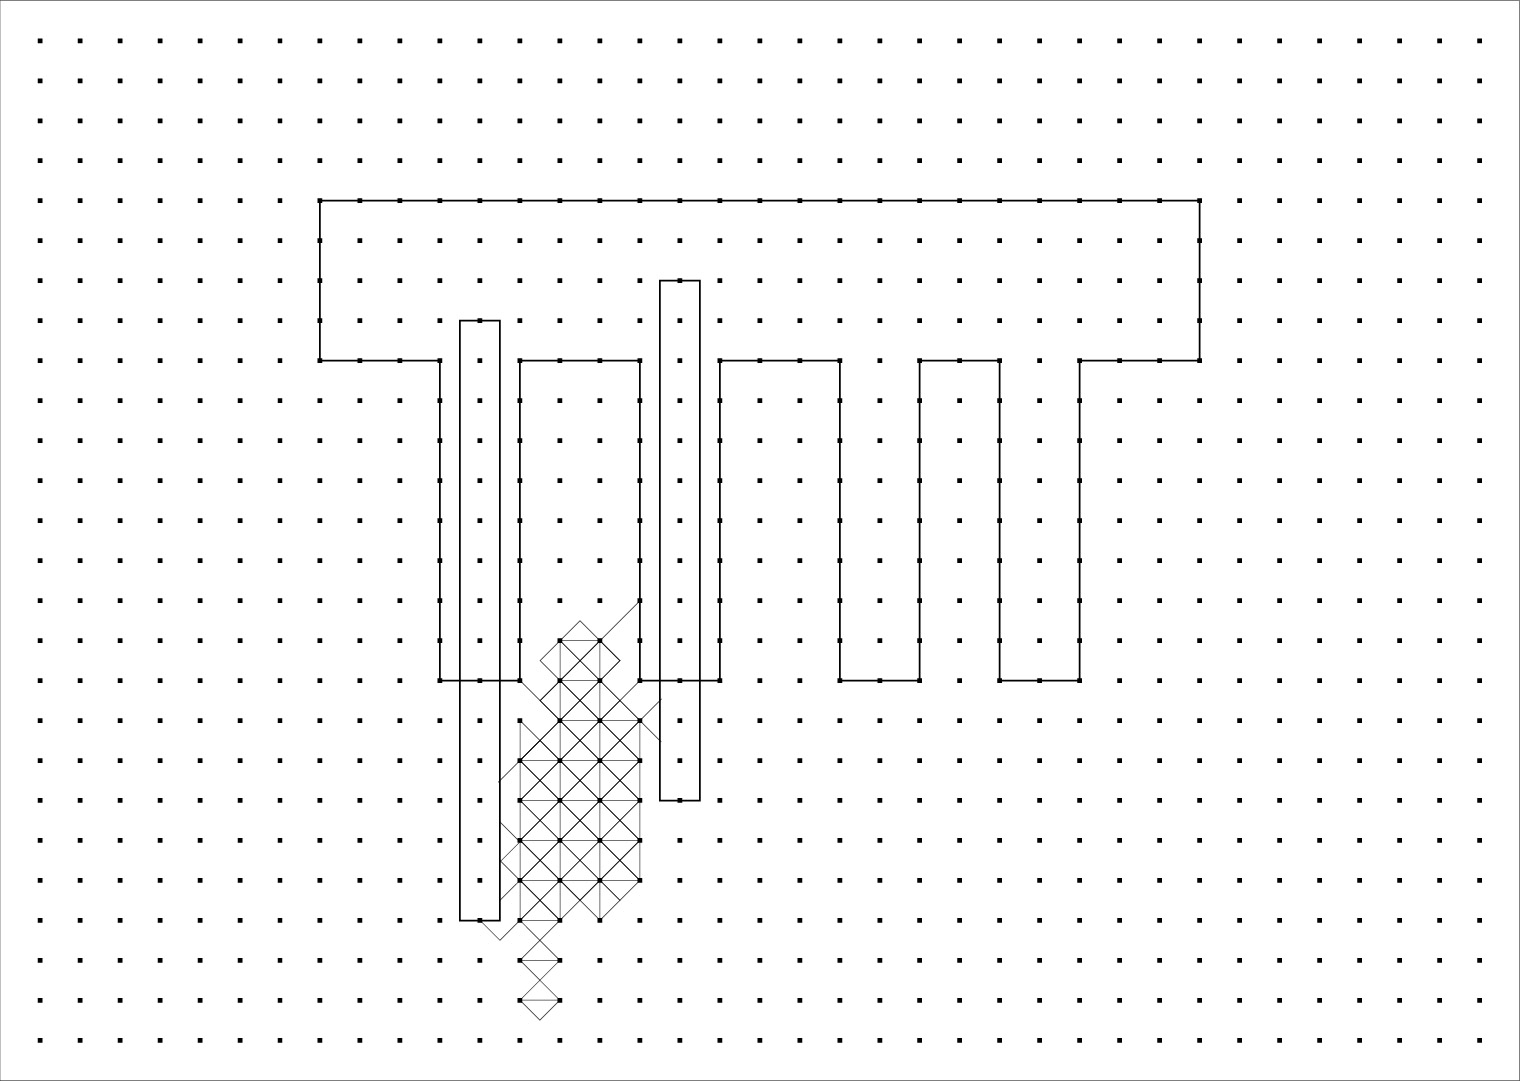
\includegraphics[width=1\textwidth]{pictures/JoiIllustr_V3-04.jpg}
 \caption{``Antidisciplinary people'' are also looking for opportunities between the disciplines.}
 \label{fig:discipline004}
\end{figure}

\begin{figure}[h]
 \centering
 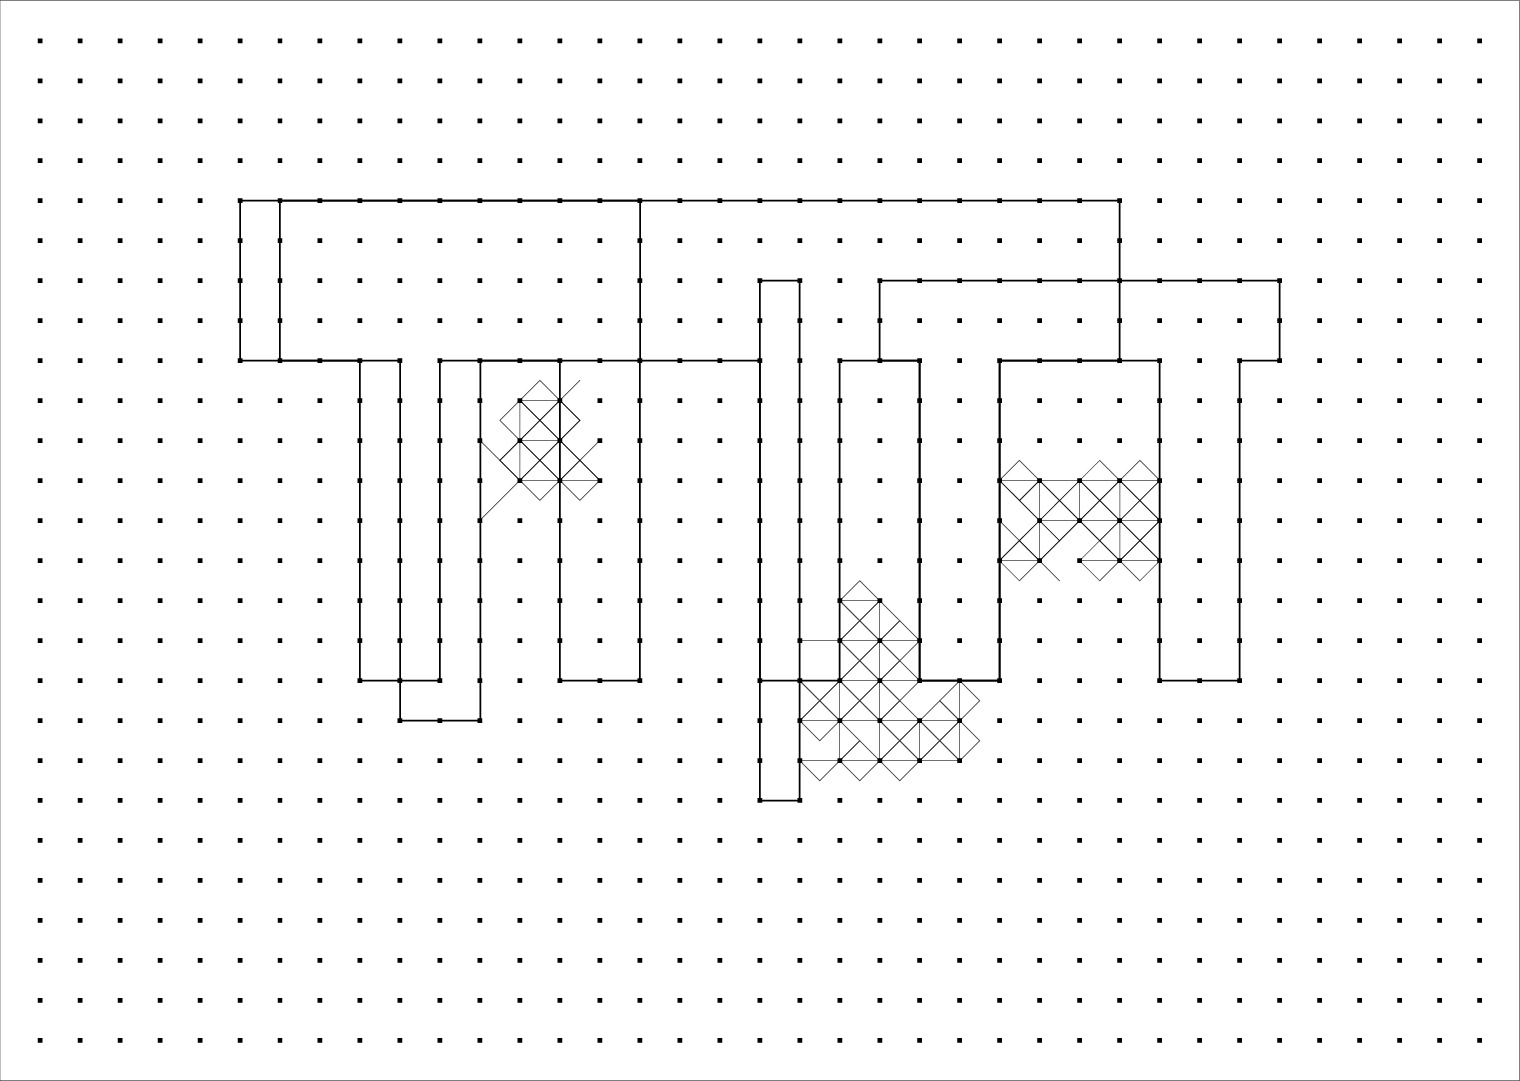
\includegraphics[width=1\textwidth]{pictures/JoiIllustr_V3-05.jpg}
 \caption{A diverse combination of I, T, $\pi$, multi-disciplinary and antidisciplinary people create a vibrant ecosystem of depth,breadth, and emergent disciplinary interactions.}
 \label{fig:discipline005}
\end{figure}

People who conduct research can be modeled as individuals in a population in an evolutionary dynamics game. While academics do care about money, their payout is often success in some combination of impact, peer validation, and the joy of discovery. While economists can model all of these payouts as a form of utility function that can ultimately be converted to monetary value, few academics calculate the dollar value of each citation when they write a paper. They are more likely thinking about their progression through the academic system, heading toward a degree or tenure. They are also likely to be thinking about power and funding (getting closer to a utility function calculus), which will allow them to hire researchers and buy equipment and materials to conduct experiments that incrementally augment or perhaps overturn existing theories.

In this way, the structure of academic institutions, with their schools and departments providing degrees and tenure through a process of peer review, reinforces the focus on going deeper rather than wider --- the target of the work of most academics focusing on a very small number of people who are sufficiently advanced in a field to understand whether and how a new work contributes to the field. The structure of academic publishing, the currency in many academic fields, is also based on peer review and advancing the field roughly in the direction it is already headed. Finally, major funding sources tend to amplify these focus areas because programs are designed around the experts in each field. This produces ``I'' people who tend to be vertically focused on an Y-axis. (See \autoref{fig:discipline001})

Many experts whose knowledge is of the deep variety consider communicating with the public beneath them and a waste of time. They would rather aim at developingthe deepest knowledge in their field, and prioritize a Nobel Prize over public acclaim --- although a Nobel Prize will lead to precisely that, just along another pathway. John Brockman, in \emph{The Third Culture} \cite{brockman1996third} and through his success in developing authors of scientific books for mass audiences, showed that scientists can write for and be appreciated by the public. This created a new category of public intellectual --- the more traditional academic researcher with a public audience. It also led to the development of more ``T'' type people, whose acumen was deep but who could also communicate with the public as well as with peers in other, adjacent fields. Later, TED Talks would also serve as a way for academic researchers to reach a mass audience.

Many academics look down on the public facing presentation of academic work as necessarily shallow, but well-known scientists have disagreed. Albert Einstein famously said, ``All physical theories, their mathematical expressions apart, ought to lend themselves to so simple a description that even a child could understand them'' \cite{clark2011einstein}.

Human beings have a limited amount of time, and while some people can get more done in their life than others, there is a bounded amount of space your personal shape can take, so there are inherent trade-offs in going deep in a single discipline, deep in multiple disciplines, or going broad across many disciplines.

Some academics are deep in two disciplines and can connect them and bring together ideas as well as specialists from those disciplines through translation of each discipline's vocabulary. These are \(\pi\) people, the interdisciplinarians. Those who have proficient, but not quite as deep, knowledge in multiple fields are ``M'' people -- multidisciplinary. (See \autoref{fig:discipline002}) Some interdisciplinarians and multidisciplinarians also spend time exploring the space between disciplines or at the intersections of disciplines. (See \autoref{fig:discipline004}) These areas tend to attract less funding, have fewer peers and, subsequently, have less existing prior work overall. Those factors make these areas harder to explore, and there is furthermore a great risk of becoming an academic orphan without collaborators, a tenure path, or a job market. 

But these new spaces offer tremendous opportunity. The key to success at the Media Lab is that we are able to deploy funding for exploratory work in the areas that fall between disciplines through a unique consortium funding model. The model pools money from funders that is then distributed among the Lab's researchers without direct control from the funders. The consortium encourages the students and faculty who are funded to explore in an undirected way. We have our own academic program that allows us to provide tenure and Master's and PhD degrees in the program in Media Arts and Sciences, sometimes called the ``department of none of the above'' --- a kind of disciplinary heterotopia (from the Greek for ``other place'') as described by Foucault \cite{foucault_order_2002}. 

\marginpar{In fact, we like to think that all of the Media Lab is a heterotopia. In part, this is because our focus on making and deploying things as a research method allows us to collaborate with other departments and outside academics that we don't necessarily overlap with epistemologically. In the process of making things, we are able to be rigorous in a different way --- through practice --- and we can learn through doing.}In fact, we like to think that all of the Media Lab is a heterotopia. In part, this is because our focus on making and deploying things as a research method allows us to collaborate with other departments and outside academics that we don't necessarily overlap with epistemologically. In the process of making things, we are able to be rigorous in a different way --- through practice --- and we can learn through doing.

This allows us to create an ecosystem of I, T, \(\pi\) and M and antidisciplinary types that feeds new ideas into existing disciplines and supports the emergence of intersectional disciplines as well as completely new ones. This breaks down silos. (See \autoref{fig:discipline005}.)

In ``Enthnocentrism of Disciplines and the Fish-Scale Model of Omniscience'' \cite{campbell1969ethnocentrism} Donald Campbell describes the tribalism or in-group partisanship of disciplines and suggests a pattern of overlapping disciplines in a kind of fish-scale pattern to create a comprehensive social science or a multiscience. (See \autoref{fig:fishscale1} and \autoref{fig:fishscale2}.)

\begin{figure}[h]
 \centering
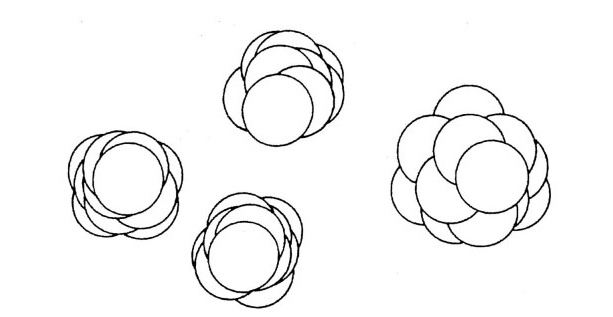
\includegraphics[width=1\textwidth]{pictures/fishscale1.jpg}
 \caption{``Present situation: Disciplines as clusters of specialties, leaving interdisciplinary gaps'' \cite{campbell1969ethnocentrism}.}
 \label{fig:fishscale1}
\end{figure}

\begin{figure}[h]
 \centering
 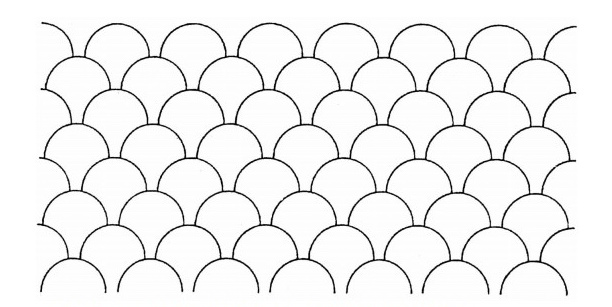
\includegraphics[width=1\textwidth]{pictures/fishscale2.jpg}
 \caption{``Ideal situation: Fish-scale model of omniscience'' \cite{campbell1969ethnocentrism}.}
 \label{fig:fishscale2}
\end{figure}

Ed Boyden who runs the Synthetic Neurobiology Group at the Media Lab,  and I are discussing a more radical approach --- the next step beyond antidisciplinarity as a connector and a generator of new disciplines. In this new way of thinking, instead of a disciplinary approach to the creation of knowledge, Boyden describes a goal-oriented approach --- in his case, understanding and controlling the brain --- and works backwards to tap into or create new disciplines to generate the tools. From an evolutionary dynamics perspective, his payout and motivations are very different from disciplinary communities, even though they overlap with them. For Boyden, it is a completely different dimension from which to understand and structure the world --- much like the sphere that crosses Flatland \cite{abbott1884flatland}. In a way, Boyden is trying to create a new architecture inside of a heterotopia for his community.

\begin{figure}[h]
 \centering
 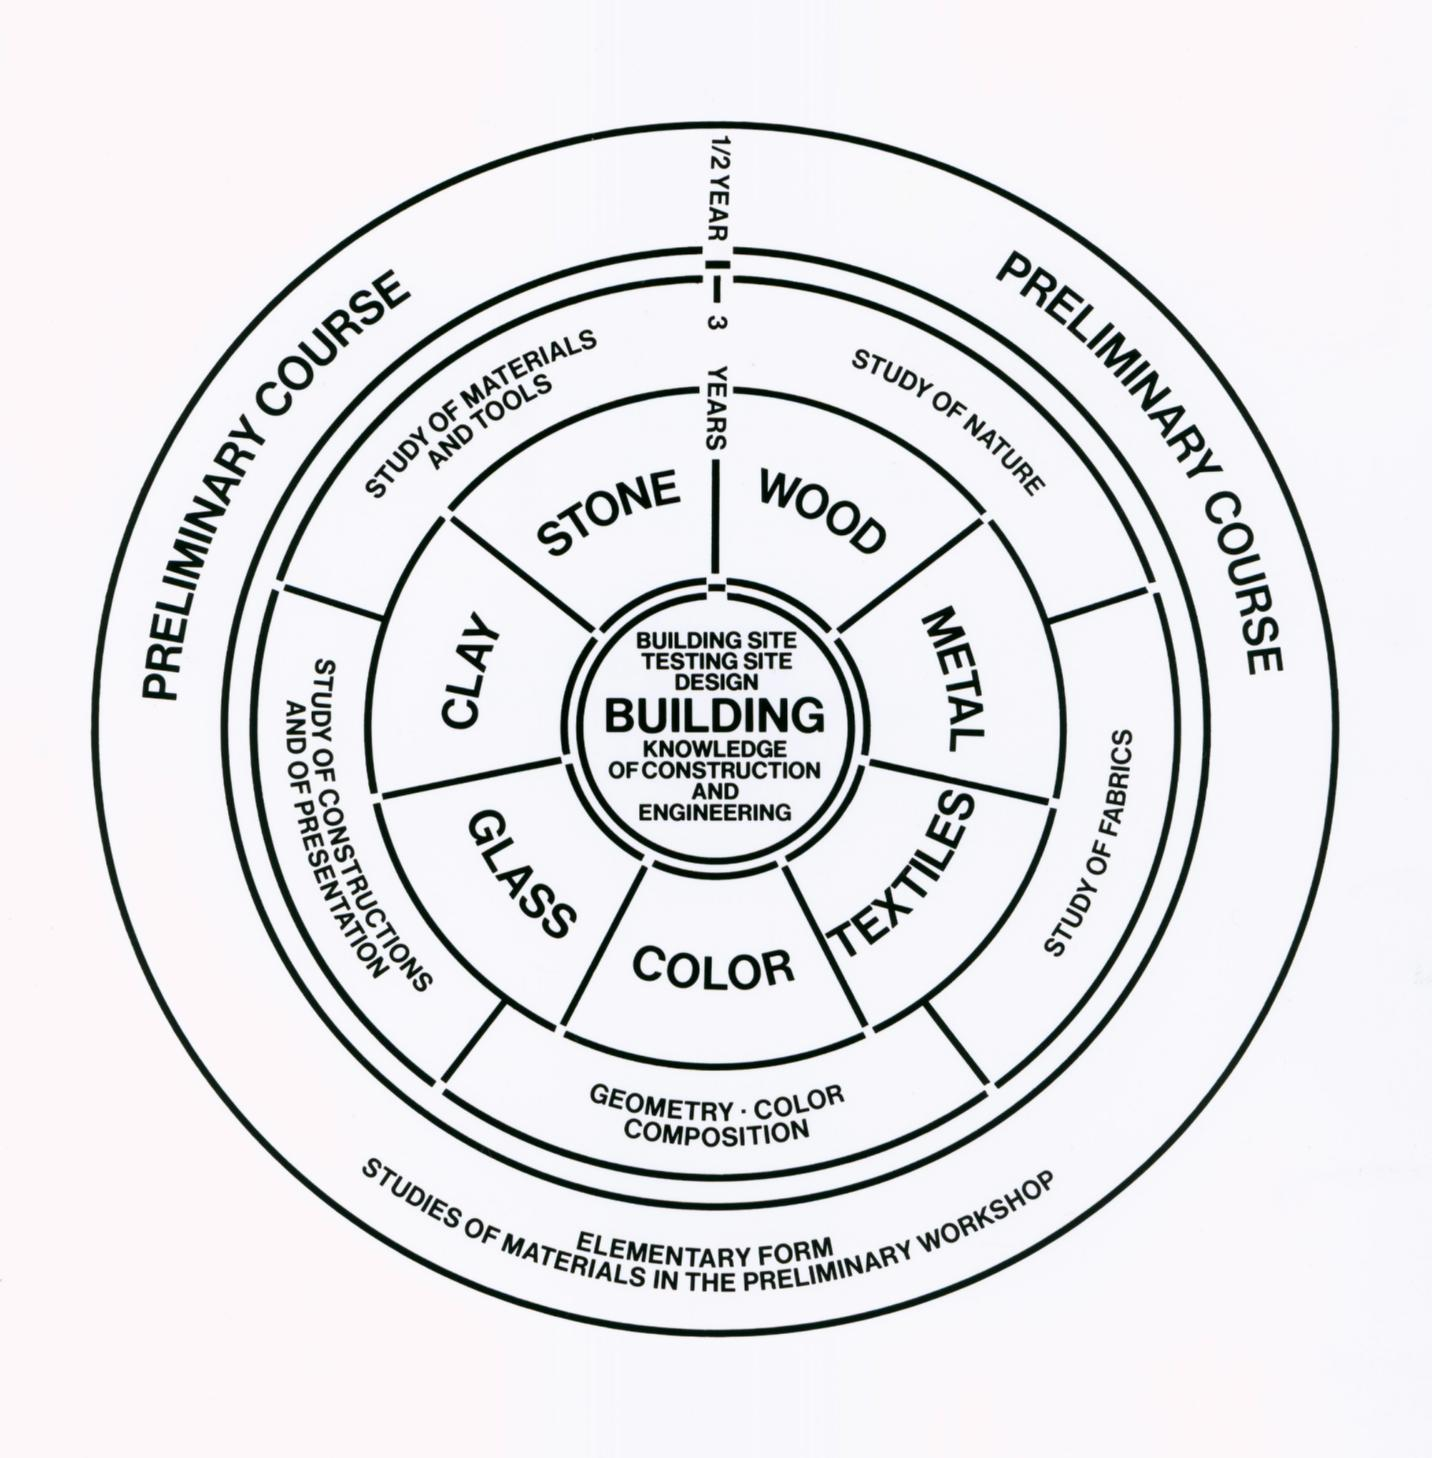
\includegraphics[width=1\textwidth]{pictures/bauhaus-curriculum-diagram}
 \caption{Diagram for the structure of teaching at the Bauhaus. Source: Walter Gropius, 1922.}
 \label{fig:bauhaus}
\end{figure}

\begin{figure}[h]
 \centering
 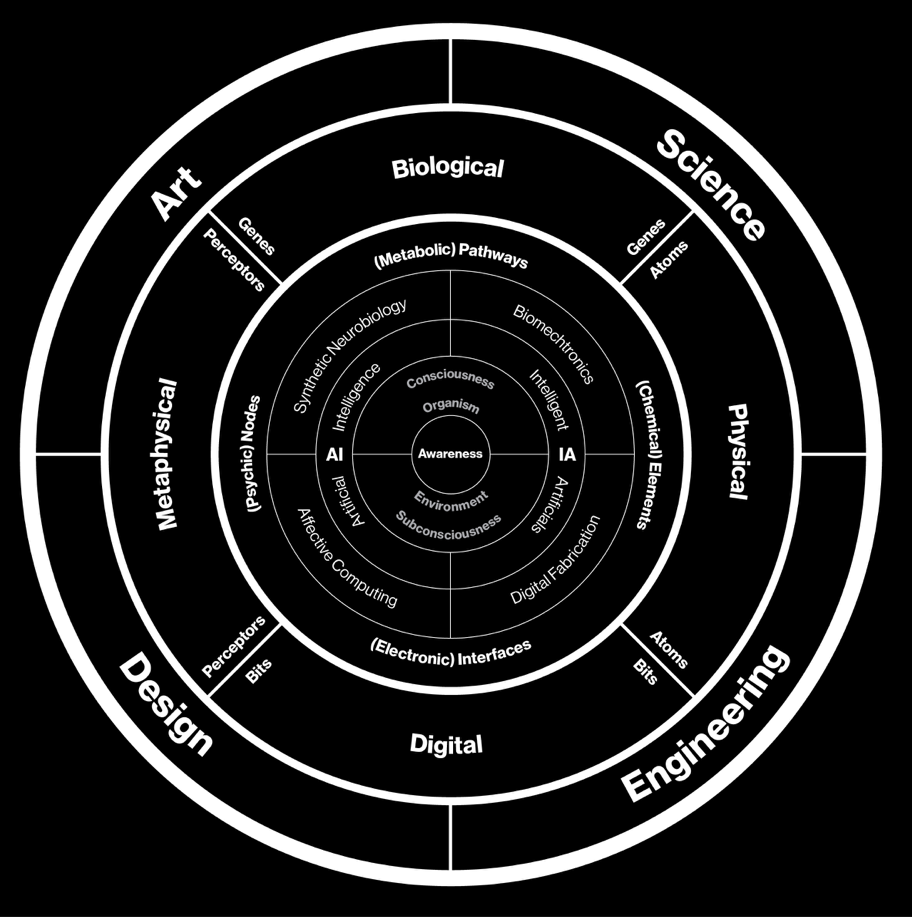
\includegraphics[width=1\textwidth]{pictures/krebs3}
 \caption{Krebs Cycle of Creativity III - Practice. Source: Neri Oxman, March 2018.}
 \label{fig:krebs3}
\end{figure}

\autoref{fig:bauhaus} is a diagram of the structure of teaching at Bauhaus in the 1920s. The Bauhaus brought together an interdisciplinary collection of disciplines, new materials and a new sensibility. In addition to a curriculum, the movement create a new style and form of architecture with real impact on the world.

Similarly, \autoref{fig:krebs3} is the third iteration of Neri Oxman's Krebs Cycle of Creativity. She is proposing a synthesis of disciplines, approaches and a sensibility that might be a way to create a new meta-discipline with a completely new way forward.

\marginpar{This inevitably requires challenging the institutions that have developed to support the academic process. We need to think about the structure of these institutions and how we might re-imagine them in the post-Internet era.} This inevitably requires challenging the institutions that have developed to support the academic process. We need to think about the structure of these institutions and how we might re-imagine them in the post-Internet era.


\subsection{Decentralization and Layers}
\label{decentralization}

The Internet, especially the early Internet, was a great example of the transformation of slow, powerful and incumbent institutions shown in figure \autoref{fig:monolith} into a vibrant and generative ecosystem.

Breaking up telecommunications' monolithic companies and monopolies required a new architecture of layers that unbundled the control at each layer. This allowed ecosystems of competitors and collaborators to form, decentralized control and innovation at the commercial layers, and creating an open and inclusive process at the protocol layers.

The Internet unbundled the layers technically and business-wise, allowing competition and innovation to flourish. This layering allowed the unbundling of power, interoperability, competition, and the highly generative Internet.

\begin{figure}[h]
 \centering
 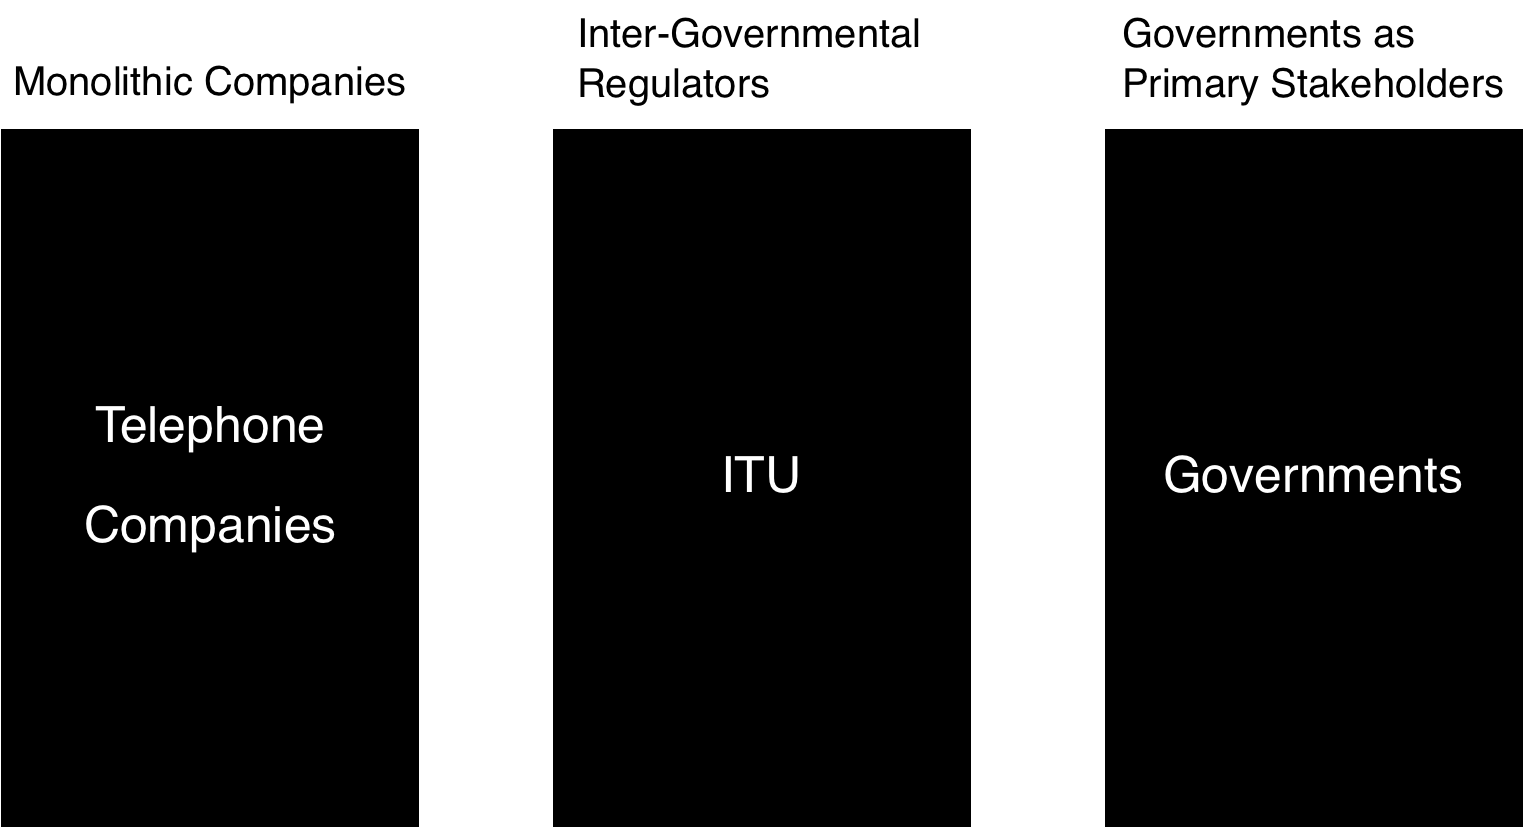
\includegraphics[width=1\textwidth]{pictures/monolith}
 \caption[Structure of telecommunications ecosystem before the Internet.]{Before the Internet, the telecommunications industry was monolithic telephone companies, working with inter-governmental regulators like the United Nations and the International Telecommunications Union and the governments themselves, creating a slow, bureaucratic, expensive, and closed system.}
 \label{fig:monolith}
\end{figure}

\begin{figure}[h]
 \centering
 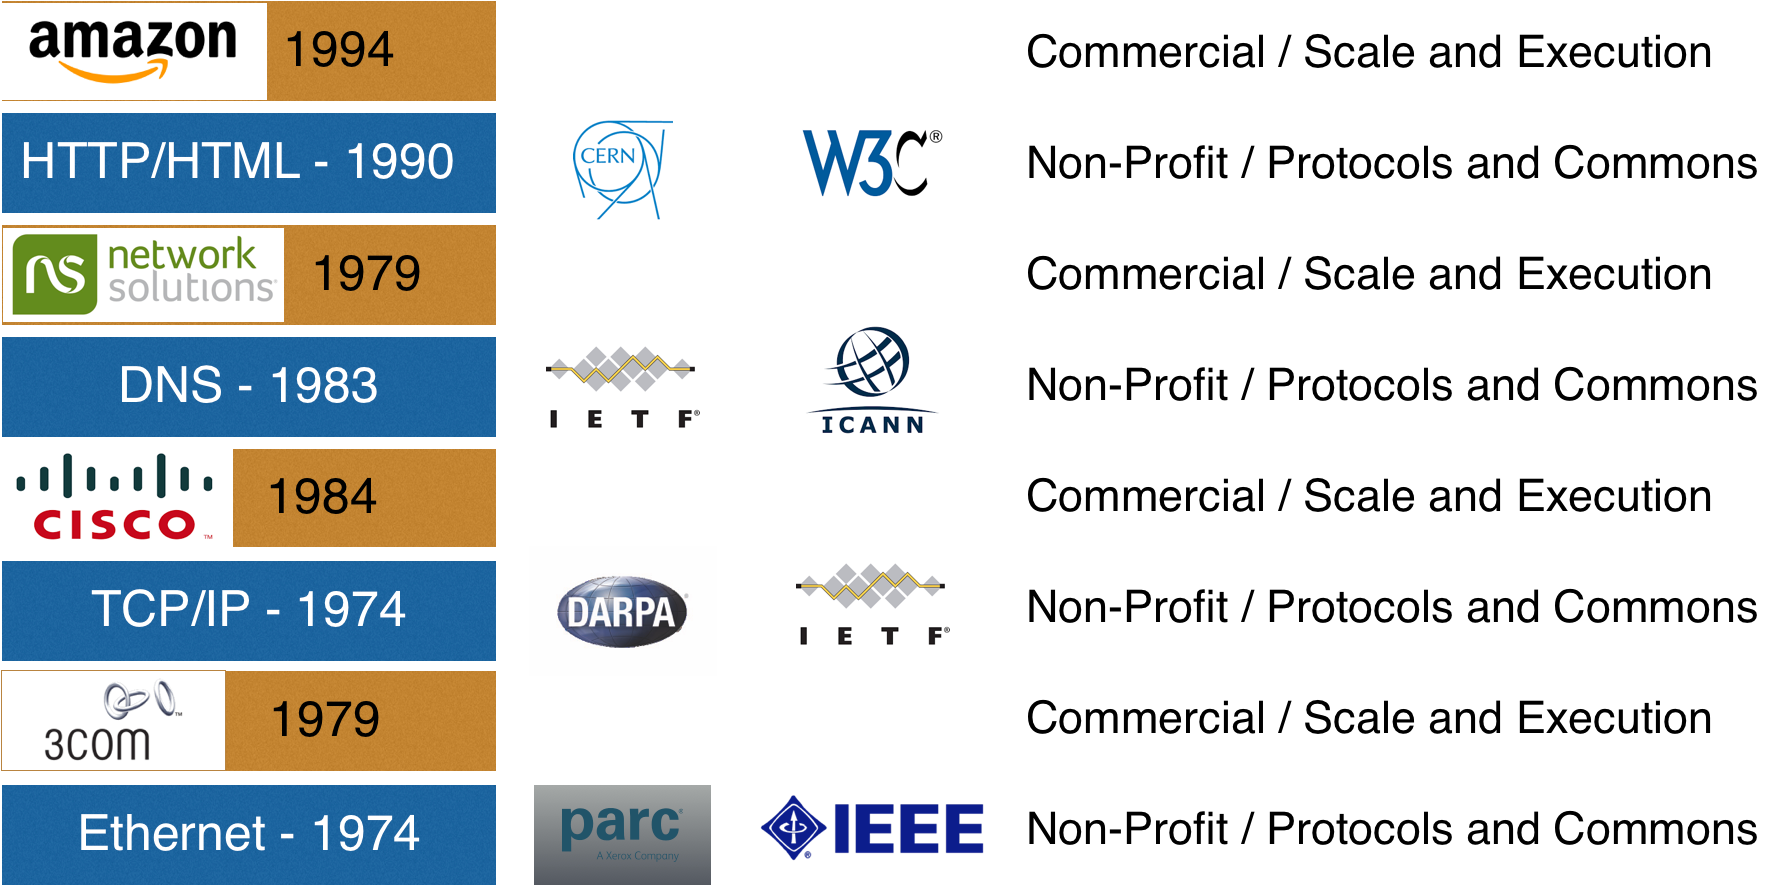
\includegraphics[width=1\textwidth]{pictures/InternetLayers}
\caption[Structure of telecommunications ecosystem after the Internet and its layers.]{The first column in this figure are the layers of open protocols and examples of companies creating the ``layer sandwich'' of the Internet. The next column is the funding or research organization that originated the protocol. The next column is the non-governmental not-for-profit standards body that currently stewards the protocol. The column on the right shows the role of that layer. The Internet unbundled the layers technically and business-wise allowing competition and innovation to flourish. Open Protocol and not-for-profit layers allowed communities of experts to design the best social and technical solutions without being encumbered by business and political interests. Commercial layers using these new open protocols were able to flourish and compete using the protocols to communicate with but be free from encumbrance from the layers above and below. This layering allowed unbundling of power, interoperability, competition and the highly generative Internet.}
\label{layertable}
\end{figure}

The personal computer and the Internet pioneered and perfected an architecture of unbundling the layers of a system --- chips, firmware, hardware, operating system, software, dark fiber and wire, modem, Ethernet, \ac{TCP/IP}, \ac{HTML}, website, browser. Each layer of the Internet (although PCs have similar layers) has an open protocol and standards stewarded by a non-governmental, not-for-profit organization with general but very clearly defined application programming interfaces, or \ac{API}s. Open protocol and not-for-profit layers allowed communities of experts to design the best social and technical solutions without being encumbered by business and political interests. Commercial layers using these new open protocols were able to flourish and compete using the protocols to communicate with, but be free from encumbrance from, the layers above and below. The system is decentralized. This architecture has significant advantages over monolithic systems in terms of efficiency and lower cost, resilience, interoperability of different technologies at each layer and the ability to continuously innovate rapidly.

\subsubsection{The Internet, Decentralization, Unbundling}

Before the Internet, telecommunications was centralized in monolithic telecommunications corporations. They controlled everything from pipes and wires to content. When multimedia first emerged, cable companies ran interactive video experiments and telephone companies like France Telecom and \ac{NTT} ran experiments such as Minitel and Captain.

The Internet was successful because we were able to unbundle its layers and create open and interoperable standards that allow companies to compete and create strong operational layers between open protocols. The key to open protocols was non-governmental coordinating organizations, such as \ac{ICANN} and \ac{IETF}. The \ac{API}s and protocols for communications between the layers was also essential.

The inventors of the protocols, such as Sir Tim Berners-Lee who created \ac{HTML} at \ac{CERN} and the team of academics who created \ac{TCP/IP} many years before, deliberately didn't patent their inventions. Instead, they established not-for-profit and non-governmental stewardship organizations to support a community of technical people and a process of coordination with stakeholders, as well as with similar \ac{NGO}s in other layers. They built interoperable systems that allowed systems and services to communicate with and build on top of each layer. These layers relied on consensus and were the essential ``commons'' of the Internet.

\marginpar{The primary risk, as we now see, is that while open protocols allow competition, they also allow companies to scalably harness the network effect \cite{web20} and we have seen monopolistic companies emerge in each of the commercial layers as a result.}It is notable that all of this original work was primarily academic and didn't involve governments except funding from \ac{DARPA} for early work in \ac{TCP/IP}. Government and traditional telecommunications attempts at creating something similar ended up in protocols such as \ac{X.25} that were complicated and encumbered by business and political interests that made them much less effective than the Internet protocol and lacked the fundamentally community-oriented and humble approach that made the Internet technical communities so generative and successful.

Built on top of these layers and between the ones above, the commercial layers of startups, mostly funded by venture capital, took open standards and scaled them and made them valuable and accessible to the public such as 3Com with Ethernet, Cisco with \ac{TCP/IP} and the browsers with \ac{HTML} (although Firefox is a notable not-for-profit example). For scaling and execution, for-profit, market-oriented ventures are extremely effective. The interoperable layers created a fertile platform for fair competition and disruption and allowed the emergence of companies such as Cisco on top of \ac{TCP/IP} and Amazon on top of \ac{HTML}. (See \autoref{layertable})

The primary risk, as we now see, is that while open protocols allow competition, they also allow companies to scalably harness the network effect \cite{web20} and we have seen monopolistic companies emerge in each of the commercial layers as a result. Nonetheless, so far even the biggest tech monopolies are eventually disrupted as technology advances, user behavior changes and new ventures come along to disrupt it --- Yahoo and Microsoft appeared to be indestructible monopolies until they weren't. However, Facebook and Google appear to be sustaining their stature so far.

Unbundling and interoperability has allowed the creation of a generative ecosystem that has thrived thanks to a kind of ``permissionless innovation.'' This was nurtured in great part by the diminishing cost of communication, collaboration and distribution, which helped sustain communities that generated the production of free and open source software. This greatly diminished the cost of innovation and pushed it out to the edges, into dorm rooms and to individuals who wanted nothing to do with large companies and traditional institutions.

I think unbundling and thinking of ecosystems in terms of layers linked by protocols controlled by open and inclusive nonprofit organizations is  applicable to many other vast systems including finance, virtual reality, international relations, government and artificial intelligence.

These organizations and communities can bring everyone together to coordinate the necessary relationship between government, markets, society and technology.

\subsection{Reinventing Health Care}
\label{theoryhealth}

\marginpar{As the Internet fundamentally changes the way that we see and interact with each other and the world, advances in artificial intelligence and machine learning are fundamentally changing how we understand and interact with health and medicine.}As the Internet fundamentally changes the way that we see and interact with each other and the world, advances in artificial intelligence and machine learning are fundamentally changing how we understand and interact with health and medicine.

To break through the impasse we have reached in determining the future of the pharmaceutical industry and to understand and develop diagnostic and therapeutic capabilities requires application of the antidisciplinary approach to the human body and health.

We must discover new inventions and paradigms to treat the diseases that we face, and create new tools. This requires abandoning the silos of disciplines and bringing all disciplines to bear on understanding health and designing a new structure for innovating to come up with solutions. To implement this vision, I have brought together mathematicians, physicists, systems biologists, computer scientists, new tools for visualizing and interrogating systems, and many others to try to get a better understanding of the science and how these systems work. We must question our basic assumptions and possibly invent new mathematics to model biological systems. We need to understand how to apply artificial intelligence and machine learning for understanding the systems, as well helping us create new diagnostic and therapeutic tools. In addition, the clinical trials for deploying new technology must be redesigned; using new tools such as machine learning and data science could significantly improve the way we test new methods. 

This cannot happen with the current structure of government funding and the discipline-segregated research university system. With the maturing of new technologies, the opportunity to evolve new paradigms for the future of health is here. We are already seeing signs of more streamlined processes; the ability to have new clinical endpoints, and greater insights into the patient experience via sensors. The application of such digital tools has generated data pools that have the potential to be explored via \ac{AI} and machine learning approaches. These new approaches will allow for a new development paradigm that will enable therapies and cures to be more targeted to individual patients and be delivered faster to market. For example:

\begin{enumerate}
\item In 2018, the 21st Century Cures Act was signed into law, a significant bipartisan legislative achievement aimed at accelerating the discovery, development and delivery of new cures and treatments. The Act issued an important directive to the FDA for the design and qualification of drug development tools, defined as biomarkers,  clinical outcome assessments, and any other method, material, or measure that is determined to aid drug development and regulatory reviews. It also advanced the idea of an ``information Commons'' for sharing data \cite{21centdatashare}. The law places heavy emphasis on leveraging innovation, advancing digital health technologies and developing next generation analytical approaches to improve health care, broaden access and advance public health goals. We are poised to enter an era of exponential growth of new machine learning, \ac{AI} and gene editing techniques for biological, preclinical and clinical research problems. Health and pharmaceutical companies could benefit vastly by using \ac{AI}-based generative, classification and prediction tasks to solve their most important challenges. Two specific examples of advanced analytics that could leapfrog the drug development process, in synergy with the Cures act, are listed below:

\begin{enumerate}
\item Complex systems-level datasets created from next-generation sequencing, transcriptomics, proteomics, metabolomics and single-cell experiments from patient samples and animal models can be processed with \ac{DNN} architectures.
\item High-throughput screens geared towards small-molecule discovery use manual processing, and in silico\footnote{\textit{In silico} is means ``performed on computer or via computer simulation.'' The phrase is an allusion to the Latin phrases \textit{in vivo}, \textit{in vitro}, and \textit{in situ}, which are commonly used in biology \cite{wikipedia:insilico}.} prediction of hits and potential targets and mechanisms. These tasks could be automated as new generative \ac{AI} systems can be used to design effective small molecule candidates.
\end{enumerate}
\end{enumerate}


\subsection{Lessigian Quadrants}
\label{sec:lessigq}

In his book, \emph{Code and Other Laws of Cyberspace} \cite{lessig2009code}, Lawrence Lessig describes four quadrants --- law, markets, norms and architecture (See \autoref{fig:lessigian}) --- as the four factors that influence what an individual can do. Architecture, in his definition, is the technical architecture, and he explains that laws can affect norms, markets and architecture. As an example he considers ways to get people to drive more slowly down a street. You could install speed bumps, a technical intervention, or you could establish a more stringent speed limit and enforce it, a legal intervention. You could also perhaps make it socially unacceptable to speed down the road, which would involve norms, or perhaps reward drivers financially for slowing down, a market solution. 

\begin{figure}[h]
 \centering
 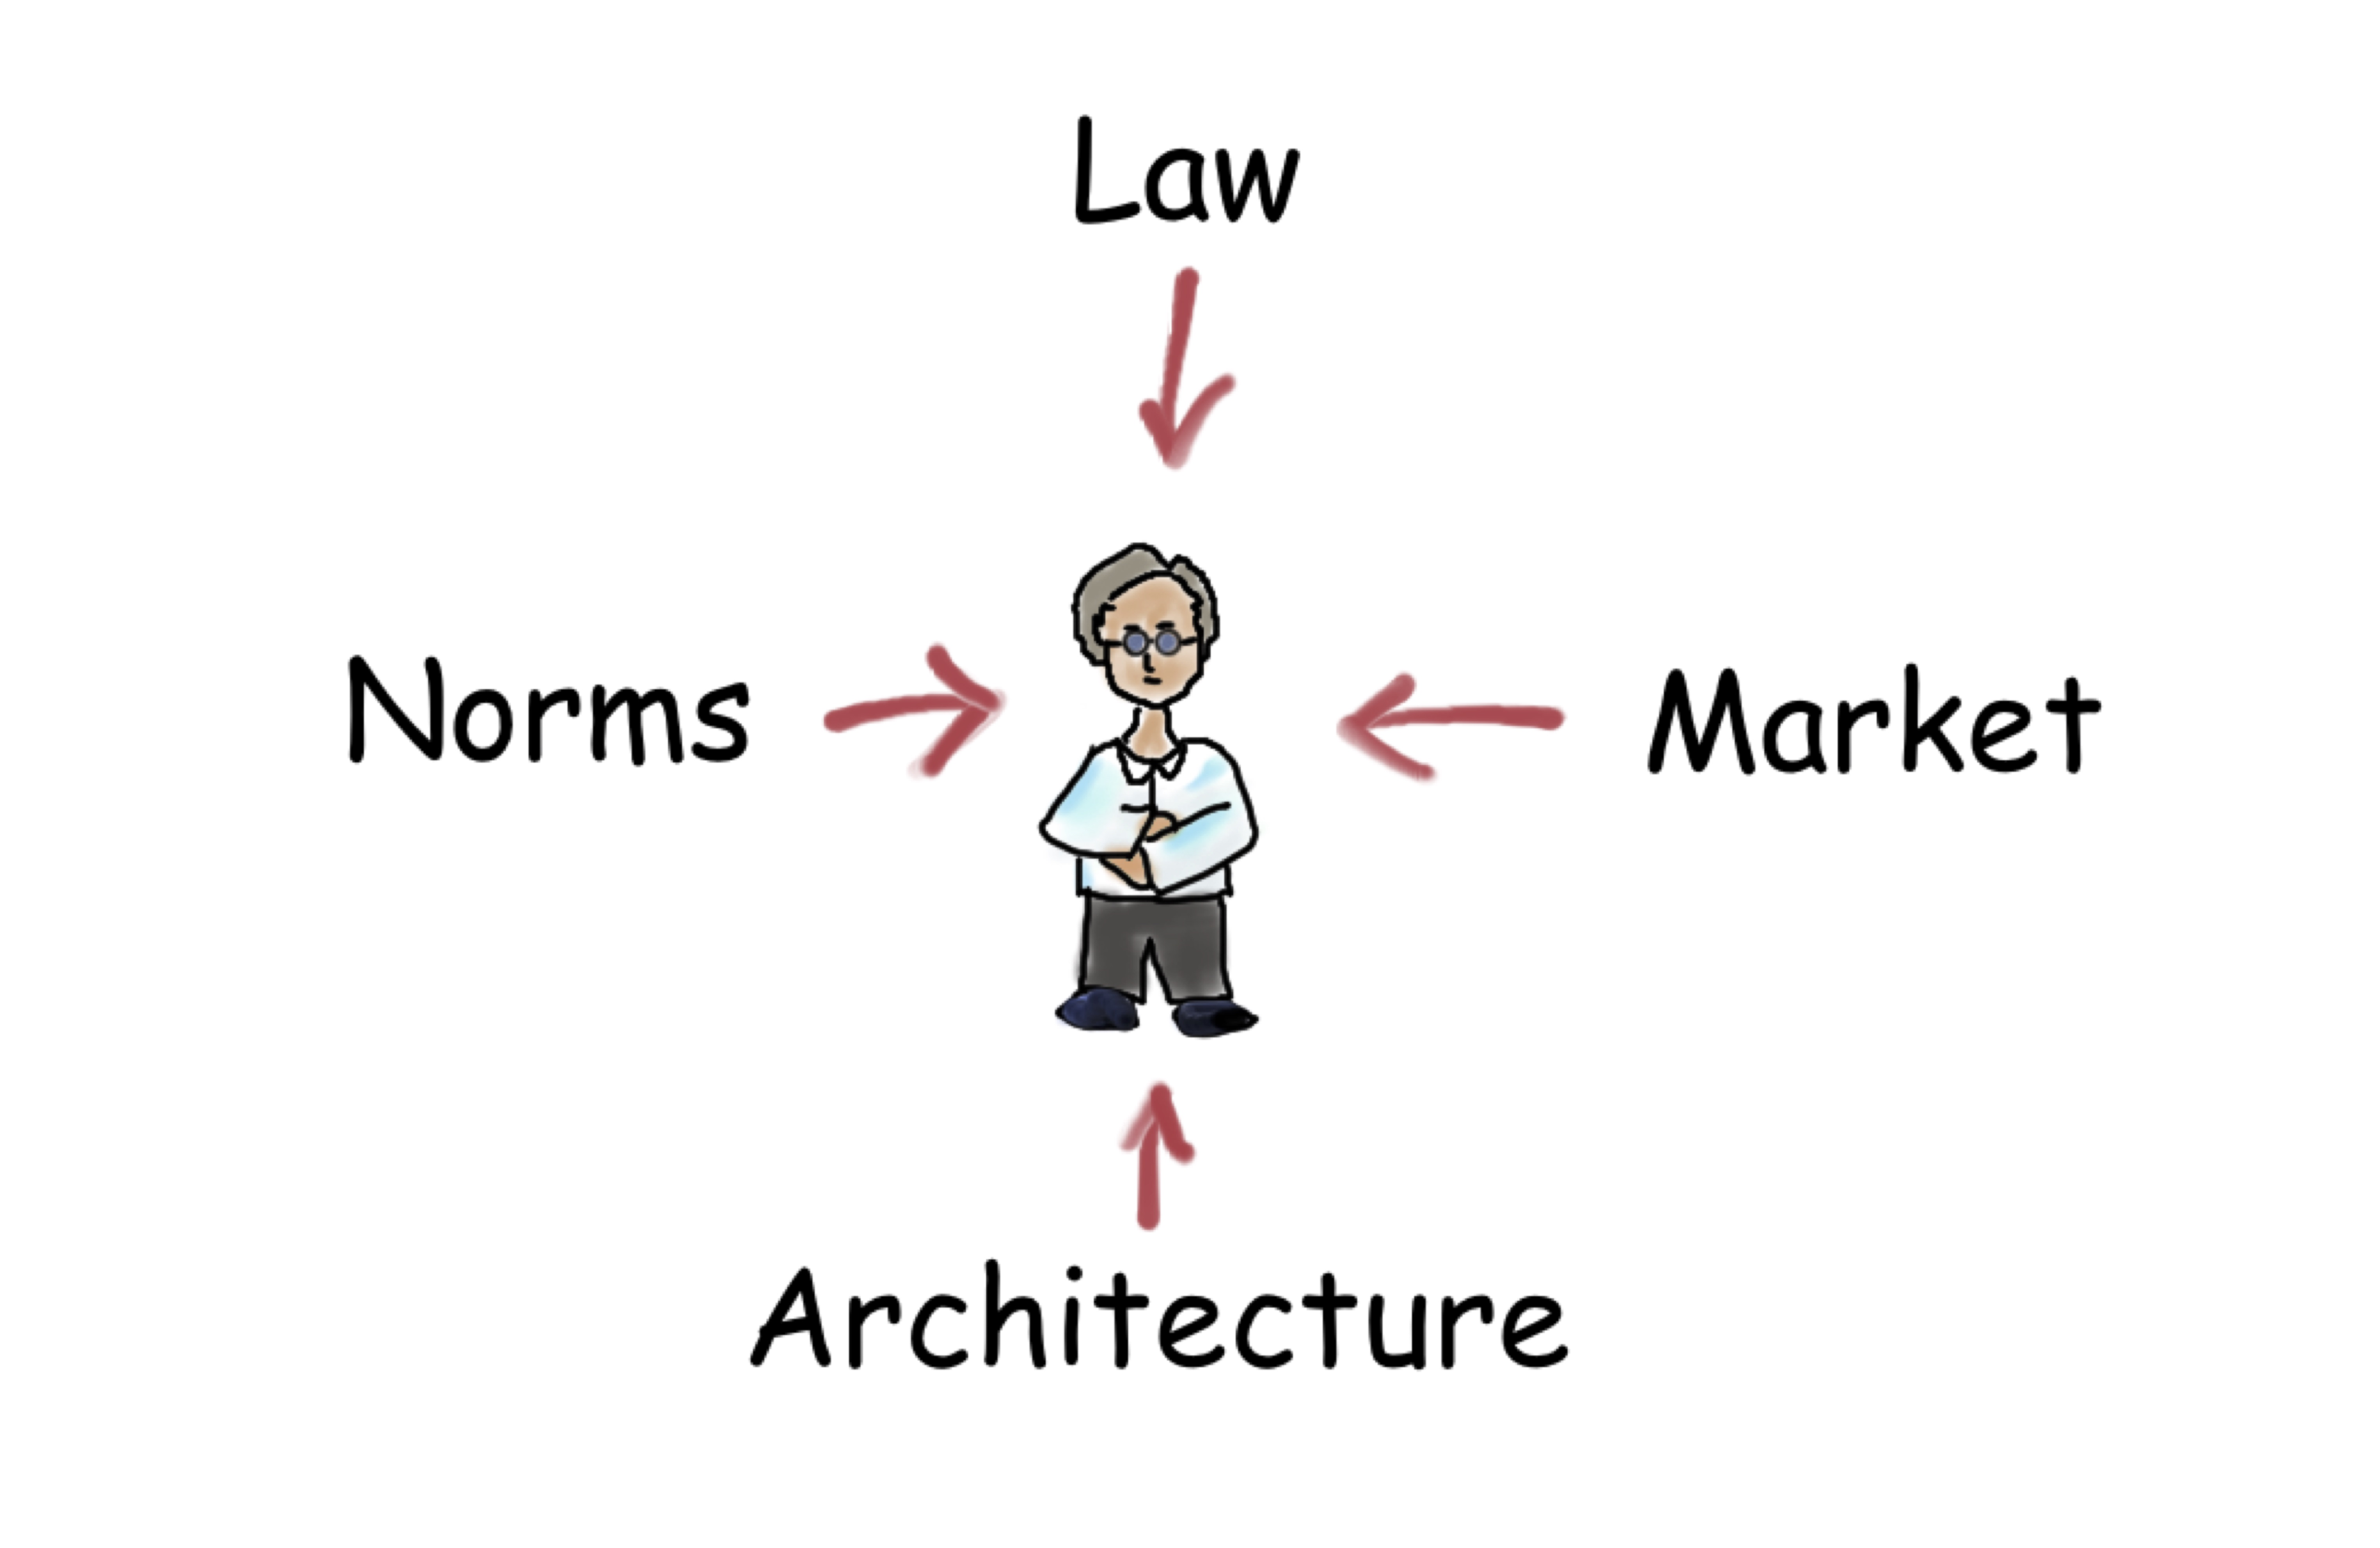
\includegraphics[width=.5\textwidth]{pictures/lessig.jpg}
 \caption{Lessig and the four quadrants. Image by Iyad Rahwan.}
 \label{fig:lessigian}
\end{figure}

One of the key points of Lessig's book is that a combined understanding of technical code and legal code became necessary for designing an appropriate legal and technical infrastructure once platforms such as the Internet emerged. For example, when the Internet made it possible to copy music and other copyrighted media, services such as Napster made it technically very easy to share music. Hollywood reacted by passing strict laws and enforcing them. This diminished the ability to share and remix creative works on the Internet. Eventually, Apple Inc. made a market intervention by building iTunes, which made the experience of sharing music legal and technically simple at a reasonable price --- and created a financial bonanza for itself by putting the company in an advantageous position in the market.

Around the same time, the record labels went after sampling, a key component of hip hop music. As they started suing artists who sampled, people stopped sampling as much. This changed the norms and in the US with common law, the norms changed the interpretation of the law. The norms of society were forever changed, and sampling music became illegal. Remix as a musical art form in the US was stopped dead in its tracks.

In other places, such as Brazil, things played out very differently. Markets and cultural norms actively promoted sharing, sampling and remixing, and focused on live performances to generate revenue. The event producers funded artists and the distributions of copies of the music were not policed \cite{shaver2010access}.

The upshot of Lessig's argument is that the four quadrants need to coordinate with each other, and incorporating all four quadrants at once is likely to yield the most effective and appropriate approaches to managing the development and deployment of technology in our society. This requires more than just a bit of interaction and negotiation between the quadrants, but rather an approach that goes beyond traditional disciplines --- an antidisciplinary approach.

\marginpar{Lessig's quadrants and an antidisciplinary approach are required for developing new rules as well as fixing broken ones.}Lessig's quadrants and an antidisciplinary approach are required for developing new rules as well as fixing broken ones.

%\subsection{Fixing Broken Protocols}
%
%As technologies change, many of the laws and regulations that made sense in the past, stop making sense. In the following essay from 2017, I describe a number of laws from money laundering to copyright to wiretapping and how the way in which they are broken is similar and how a Lessigian approach is necessary to fix them.
%
%\emph{Original title:
%\textbf{Why anti-money laundering laws and poorly-designed copyright laws are similar and should be revised}} \\
%
%\emph{Originally published October 13, 2017} \\
%
%\emph{Abstract: Intentionally or unintentionally, poorly crafted or outdated laws and technical standards threaten to undermine security, privacy and the viability of our most promising new technologies and networks, such as Bitcoin and the blockchain. We should vigilantly be reviewing and revising laws and standards for the public good and working to prevent the creation of fragile and cumbersome systems designed to comply with these poorly crafted or outdated laws. In this post, I discuss the Digital Millennium Copyright Act's Anti-Circumvention provision, Digital Rights Management, Anti-Money Laundering Law, Know Your Customer Laws and security backdoors.} \\
%
%The Internet's founding principles --- openness, unbundling, diversity, open standards --- made it robust, a force for democratizing access. That access created an explosion of innovation far beyond anyone's imagination.
%
%The Internet's openness is its strength. It is a ``stupid network'' \cite{isenberg1997rise} whose internals are unbundled into layers of open standards that sandwich layers of diversity and innovation. Stupid networks focus on transporting bits from one place to another. That end-to-end principle allows for innovation at the network's edges. By ``unbundling'' the transportation of bits from the provision of services, applications can be developed without permission. This is where we get the innovation in services that the network's architects and managers never imagined or had to plan for.
%
%There is a perennial call to ``make the network smart.'' Someone always wants to optimize it, establish ``quality of service'' mechanisms --- for example, to make voice calls more reliable. But whenever you optimize the network for one thing, you risk de-optimizing it for another. It turns out that just adding more bandwidth has been cheaper than making the network ``smarter.'' (This argument --- that you fix networks by making them faster, not smarter --- is key to understanding net neutrality.)
%
%Policy makers grapple with the nature of the open Internet with varying results. Sometimes they'll pass rules or orders that ``break'' these principles or induce changes in the Internet's architecture that work against its openness. These are usually the result of pressure from law enforcement or corporate capture in regulation and standards.
%
%Here are a few of the worst offenders: rules, laws and standards that do damage to the net's architecture, exceeding any benefit they deliver for their champions:
%
%\subsubsection{The Anti-Circumvention Provision in the Digital Millennium Copyright Act}
%
%Sections 1201-1203 of the 1998 Digital Millennium Copyright Act (DMCA) make it illegal to circumvent locks that restrict access to copyrighted works regardless of whether you are actually breaking copyright law. This means that companies can use digital locks to hide content to which we should have legitimate access, and those locks have the force of law --- breaking them is a felony with a maximum sentence of five years in prison and a \$500,000 fine.
%
%It doesn't matter how legitimate your access is. You could be delving into your own car's computers, your medical implant's data-streams, or even content you created on devices you own yourself. (Farmers who gather soil-density surveys of their own fields while driving their tractors around them are not allowed to see those data unless they buy the data back from John Deere). This also inhibits research that focuses on whether the security of such systems is robust.
%
%The FDA, for example, has been trying to get medical device companies to allow hacking currently prevented by the DMCA \cite{fda_2016}. The Library of Congress has added car software to the list of exemptions from anti-circumvention \cite{selyukh_soon_2015}, but unfortunately it appears that "exemptions created under the rulemaking apply only to the act of circumvention, and not the development and distribution of circumvention tools." \cite{noauthor_exemptions_2017} Tough luck for drivers and researchers who aren't also encryption experts.
%
%\subsubsection{Digital Rights Management (DRM) \& The World Wide Web Consortium (W3C)}
%
%The W3C is currently standardizing DRM for use in \ac{HTML}5, the next generation of core Web standards. By allowing DRM to be included in the standard, we ``break'' the architecture of the Internet by allowing companies to create places to store data and run code on your computer that you do not have access to and where breaking into code on your computer would constitute breaking the law. This is both a security risk and a fundamentally fragile system where vast amounts of content and information could be lost in the future as technologies evolve and companies change.
%
%While DRM has been touted as critical for business, it is clear that people are willing to pay for streaming and licensing of content without technical protections. If someone could actually afford to pay the fees currently charged by the streaming vendors, why would they go to an illegal pirating site to download something? Netflix, Apple Music, Spotify and Pandora would most likely not even notice, nor would their users, if they removed DRM technology. While it may not be in their interest to announce the death of DRM, it's likely to die a quiet death.
%
%In the meantime, we will be left with a broken and fragile architecture, as well as browsers whose internals are off-limits to security researchers, who face brutal punishment for trying to determine whether your gateway to the Internet is secure enough to rely on.
%
%\subsubsection{Anti-Money Laundering Law (AML) and Know Your Customer Laws (KYC)}
%
%There are many laws that have been created to prevent money laundering - crimes that disguise the original ownership and control of the proceeds of criminal conduct by making such proceeds appear to have derived from a legitimate source. One of the reasons these laws exist is to track terrorists and criminals by monitoring money flows.
%
%Laws to prevent money laundering create a requirement to report transactions above a threshold (usually \$10,000), to report assets held anywhere in the world in your tax returns and for banks to ``know your customer'' and keep detailed records of who their customers are and what they are doing. Breaking these regulatory requirements is illegal. Like the anti-circumvention law, while you may not actually be laundering money, breaking these anti-money laundering monitoring systems constitutes a crime.
%
%The personal information and transaction details are collected are stored in databases, and this presents a substantial risk to society. Criminal and foreign government hackers have over and over again hacked the most protected of government databases, such as the personal information of US government employees with security clearance in the OPM database \cite{nakashima2015hacks}. In addition, these laws require banks and financial institutions to collect this information and structure their systems to allow this information to be collected, also making these systems vulnerable to attack.
%
%While access to this information can sometimes be useful in investigations, almost all of the sophisticated technology to ``catch the bad guys'' doesn't require access to the content of the messages, but rather only access to the metadata. This is evident in modern Signal Intelligence (SIGINT: the collection of data ranging from satellite communication to Internet packets), where intelligence and law enforcement agencies rely mostly on machine learning (artificial intelligence) and pattern recognition extracted from metadata, rather than from the content of the messages. (Snowden released a document revealing the state of the art of goverment SIGINT \cite{noauthor_himr_2011}.
%
%We are already seeing both research and practice in conducting SIGINT on the blockchain \cite{spagnuolo2014bitiodine}. With Bitcoin and Blockchain technology in ``vanilla'' form, the ability to perform SIGINT is actually HIGHER than traditional more closed systems. AML and KYC laws are often impossible to implement while balancing the privacy of the users because the Blockchain is potentially visible to the whole world and not under the control of the selected entities. In fact, I believe that we must not only prevent the collection of the same kind of information in traditional financial system, but we must also discuss developing technologies to prevent privacy risks from the analysis of the Blockchain. If we are to deploy Blockchain broadly, we will have to look at both AML and KYC laws and upgrading them, taking into account the new technical architecture and environment and balancing the privacy and security concerns.
%
%The traditional financial system as we know it will undergo significant changes in the future, especially if we are headed in the direction of Bitcoin and Blockchain. We cannot expect the current AML and KYC laws to work in this new dimension: these laws were conceived for closed, highly guarded systems and not for international, open, technical standards. For instance, the ``travel'' rule \cite{noauthor_funds_2010} requires financial institutions to pass personal information to the next financial institution when transmitting funds. There is currently no secure or easy way to do this on the Blockchain.
%
%Just like with the Internet, weaknesses in networks like the Blockchain propagate to countries and regions where privacy risks to users could cause significant risks to human rights workers, journalists or anyone who questions authority. The conversation on creating new AML and KYC laws for new financial systems like Bitcoin and Blockchain needs to be a global one.
%
%\subsubsection{iPhone/Backdoors}
%
%While putting backdoors on all of our communications and/or banning encryption hasn't been passed as a law, there is a precedent for what is going on with Apple and the FBI. In the 90s, as telephones were going from analog phone lines to digital, the FBI argued that it could become more difficult to serve wiretap orders on phone companies. Rather than connecting alligator clips to wires at the phone company's offices, they would have request their own backdoor on the switches the phone companies used.
%
%When the government offered to pay the cost, the phone companies accepted the deal and the Communications Assistance for Law Enforcement Act (CALEA) was born. The FBI has built an extensive data collection system on top of this system. (One distinction is that CALEA is about backdoors on the transport platform, while the current iPhone debate is about encryption on the edges of the network.)
%
%While Silicon Valley appears to be resisting the government requests more than the telephone companies did, they are under constant pressure, and as the Snowden documents have revealed, it appears that many companies have provided these back doors.
%
%While I'm sure law enforcement officers would love to have even more tools for their investigations, we already have more tools to track and monitor the ``bad guys'' than at any time in history. The problem with backdoors is that they create a fragile infrastructure. So that even if you believe that we can trust the US government and US law enforcement, this creates a weakness that can be exploited by the ``bad guys.''
%
%One great example of the backdoor that was recently found on the Juniper's ScreenOS Software \cite{green2015juniper}. It appears that the government may have created a backdoor on a key secure communication channel, but that someone else (unknown), put a backback door on it exploiting the backdoor to make it their own.
%
%In my view, the risk to everyone on the Internet caused by crippling security isn't worth the incremental increase in the ability for any government to engage in legitimate surveillance. This point was made clear by the President's Review Group on Intelligence, an expert group, which said that the US government should ``fully support and not undermine efforts to create encryption standards; (2) make clear that it will not in any way subvert, undermine, weaken, or make vulnerable generally available commercial encryption'' \cite{abelson2015keys}. These are just some examples of the ``broken'' laws and standards. If we do not work actively to prevent the passage of bad laws and standards, and fight to overturn or fix the existing ones, we will soon lose the Internet and all of the freedoms, innovation and opportunities that it represents.
%
%Some of my colleagues and members of the Internet community seem to believe that we can ignore regulators, or that regulators are fundamentally at odds with our best interest. I believe that we can't ignore regulators because they will eventually pass laws that impact the scope and the way in which the technology we are developing is deployed. I also believe that many regulators do believe in trying to strike the right balance, and to engaging with the right people in the right context to help create technical standards and laws that actually work in the real world. We have had many successes such as a relatively unregulated early Internet, but we have also made some mistakes. For instance, were able to stop some mistakes like SOPA and PIPA \cite{noauthor_protests_2018} and also the Clipper Chip \cite{levy1994battle}, but many laws such as the anti-circumvention piece of the DMCA made it through.
%
%I believe that we need to vigilantly monitor the activity of lawmakers, regulators, standards bodies and industry groups and their activities. We must constantly review existing legal and regulatory frameworks as we develop new technologies to make sure that they make sense and not default to trying to apply existing laws and regulations to new technologies without careful review from first principles.
%
%One of the reasons I am involved in organizations such as Creative Commons and am excited about helping to create the Digital Currency Initiative at MIT is because I am interested in trying to avoid mistakes that could undermine the full potential of open and interoperable networks, such as the network of trust and value that Bitcoin and the Blockchain represent. I hope to play a role in working with all parties, such as the users, the technical community, businesses and regulators in trying to develop and implement sustainable and healthy ecosystems that will not ruin the technology or our freedoms, while providing appropriate safeguards and structures for civil society, business and government.

\subsection{Aesthetics of the Internet - Context as a Medium}
\label{userrise}

The Internet is a new technology, but it is also a platform and a medium. It is a kind of place. In ``Understanding media: The extensions of man'' Marshall McLuhan famously said, ``The medium is the message'' \cite{mcluhan1994understanding}. In order to understand what that means and how we most effectively work in the age of the Internet, we must explore what the Internet is as a medium.

Since the early 90s, I served as a jury member for the Prix Ars Electronica, one of the preeminent electronic art awards and conferences. The competition and the associated symposium provided artistic and aesthetic views on new technologies and help define these  as a medium for arts and designs. As a jury member for over a decade in the Internet category, I helped guide the development of Internet art by giving awards to interesting projects that seemed to capture the essence of the Internet. Schools and artists took cues from our awards and developed the field with us.

I was a member of the first jury that created the Internet category. This was just as the web was emerging. As with other categories of Ars Electronica, many of the early winners in the Internet category were not artists.

The early computer graphics juries awarded prizes to supercomputer visualizations. Similarly, we gave awards to Wikipedia, e-cash/e-gold, Neal Stephenson and Linux. We were sometimes criticized by the art community as giving awards to things that were not ``art'' but I defended our decisions --- artists, in my view, stretch the boundaries of a medium, used the tools in ways that the creators did not anticipate and helped society understand the medium and the future of the technology.

I believe that Ars Electronica and the artists it identified helped provide a critical view of the Internet as an art medium, and provided many insights into the risks and opportunities it presented. Ars Electronica continues to provide an important lens into thinking about the future of the Internet, science, and technology.

\begin{quote}
\emph{Aesthetics of the Internet--Context as a Medium}\footnote{This is an essay that I wrote for the Ars Electronica conference catalog in 1997 \cite{ito1997aesthetics} describing what I believed to be the essential nature of the Internet.} \\

For Ars Electronica - June 19, 1997 \\

The Internet connects computers, people, sensors, vehicles, telephones, and just about anything together in a global network which is fast and cheap. This interconnectedness is the context. Context represents the way and the timing in which nodes are connected together. If content were the noun part of information, then context would be the verb part.

New forms of media and communications tend to mimic its predecessors. Carl Malamud gives the example of early television where television shows often consisted of a radio announcer and a microphone on the screen. The Internet often has been called a method of online publishing or online broadcasting. Magazine publishers tell me that Internet advertising on a computer screen doesn't compare to an excellent full page ad in a magazine. Television producers often compare gritty Internet video to the power of a excellent television commercial. The Internet as a medium is not suited for the delivery of high volumes of the same information to many people. Currently,* the Internet connects everyone together at rather low bandwidth at low cost. The Internet delivers context, and it is of this that we should be building the future the Internet.

Much of the information in today's world and on the Internet expires very quickly. Fifteen minute old stock quotes become free, instant stock quotes costing money. Yesterday's newspapers are free on the Internet, but today's (or tomorrow's) can cost you money. It is a relationship with the newspaper and its reporters that is more important than the database of old articles. Your Netscape browser will expire in weeks. Stealing an old Netscape diskette at a computer shop makes very little sense. Rather than downloading lots of software, on the Internet people remember where to find what they need, or better yet, who to ask or where to search. It is information about information about information... Just as our monetary system has become very abstract, our currencies represent something that really has no physical reality, most information on the Internet is about context, rather than content. Instead of the hard data of yesteryear that could be bound in a book, stacked in a warehouse and distributed by trucks, the information on the Internet is about being connected LIVE and about being in the right place at the right time.

Communities on the Net consist of a group of people connected to each other in the form of discussions, games, or some other form of two-way connectedness. People invest time and energy into these communities and these communities evolve into a complex aggregate of relationships between people mediated by a technology and a context. It becomes a kind of place. These communities are influenced by the underlying technology, but grow far beyond the technology itself. The technology is a kind of genetic basis on which a new organism can grow, receiving input from its environment through its participants.

Artwork, writing and other forms of content which are often nearly static in the slow moving physical world can also become living things in the fluid, high-speed context of the Internet. An interesting idea or design can quickly become a popular item to be sampled, edited and redistributed. The artist can view their work, or their child, quickly develop in something quite different from what it was originally intended to be. The original artist is the parent, but unlike a child raised in complete isolation, work on the Internet is educated and formed, for better or for worse, into a product of its environment and society. Putting work on the Internet is more like giving birth than creating a static object.

Communities, multi-user games systems, markets, search engines and router configurations are all context oriented. The aesthetic of context is the design of such context-oriented systems which are outstanding in their nature. A good context-oriented system causes the network of living connections to converge, interact and grow. It adds value to the network and attracts users and connections.

The Internet is a self-organizing adaptive system. As John Casti from the Santa Fe Institute pointed out in his talk at the Ars Electronica Memesis symposium last year, one can understand completely the process in which a complex adaptive system works, but it is impossible to predict what it does. The Internet self-organizes itself in the very interesting area between total chaos and order. Eric Hughes has called it a working anarchy. When order is forced onto the Internet such as rigid protocols or singular ubiquitous operating systems, that layer becomes very brittle and as one learns in catastrophe theory, a shock to the system can cause a huge amount of damage. One virus or bug in the system could take the whole system down. The more inefficient and diverse nature of the current memetic/software pool allows the risk to be distributed. Many small earthquakes can help prevent a catastrophic earthquake. It is the inefficiency and the small errors that can help the Internet adapt and grow without imploding or exploding.

Ordered efficient systems are also very susceptible to fluctuation amplification. With feedback going in the wrong direction, small fluctuations in economy, politics, traffic or opinion can be amplified by the super-efficient network and explode or crash. Nature uses feedback systems that dampen such fluctuations in an elegant way to contain the energy and balance the systems. This non-linear balance is becoming exceedingly more important than to make the system faster or more efficient. This balance can also be explained as the aesthetic of the context.

\marginpar{It is the use, familiarity and reproduction that makes a meme powerful and proves its aesthetic quality. The Internet artist and the meme both work in the medium of context rather than content.}Nearly complete chaos can also be found on the Internet in the sheer number of disorganized pieces of content and people. Total chaos can also be made much more useful by adding just enough context to help group the content and people into useful communities and networks.

Therefore, I would conclude that both complete order and complete chaos offer very little information, value or energy. Systems that help order chaos or disorder order are useful. In addition, the way in which these systems cause this non-chaos/non-ordered system to manifest should retain or create as much energy as possible while keeping a feedback system that prevents it from amplifying into destruction or dampening into nothing. This requires a group of rules or memes that attracts energy in the form of people, content, traffic, money, etc. and organizes this content in a way that grows and adds value. It is almost a kind of memetic engineering.

The memetic engineer/Internet artist is interested in coming up with an idea, software protocol or image that grows and evolves on the Internet. It is more about creating life than about creating a non-living piece of art. The memetic engineer seeks to have the particular meme copied and replicated where traditional artists are protective of their work. It is the use, familiarity and reproduction that makes a meme powerful and proves its aesthetic quality. The Internet artist and the meme both work in the medium of context rather than content.
\end{quote}

\section{Deploying Change}
\subsection[Resisting Reduction]{Resisting Reduction\footnote{This section is based on an essay that I wrote for the \emph{Journal of Design and Science} \cite{ito_resisting_2017} which has since become a special issue with contributed responses and plans for a book from MIT Press.}}
\label{intro:resisting}

As the sun beats down on Earth, photosynthesis converts water, carbon dioxide and the sun's energy into oxygen and glucose. Photosynthesis is one of the many chemical and biological processes that transform one form of matter and energy into another. The molecules created through photosynthesis then are metabolized by other biological and chemical processes into yet other molecules. Scientists often call these molecules ``currencies'' because they represent a form of power that is transferred between cells and processes to mutual benefit, ``traded'' in effect. The biggest difference between these currencies and financial currencies is that there is no ``master currency'' or currency exchange. Rather, each currency is useful only in certain processes, and the ``market'' of these currencies drives the dynamics that are ``life.''

As certain currencies became abundant as an output of a successful process or organism, other organisms evolved to take that output and convert it into something else. Over billions of years, this is how the Earth's ecosystem has evolved, creating vast systems of metabolic pathways and forming highly complex self-regulating systems that, for example, stabilize our body temperatures or the temperature of the Earth, despite continuous fluctuations and changes among the individual elements at every scale from micro to macro. The output of one process becomes the input of another. Ultimately, everything interconnects.

We live in a civilization in which the primary currencies are money and power. The Internet's currency is attention \cite{goldhaber1997attention} which converts to both power and money through voice and advertising. More often than not, the goal is to accumulate power and money at the expense of society at large. This is a very simple and fragile system compared to the Earth's ecosystems, where myriads of ``currencies'' are exchanged among processes to create hugely complex systems of inputs and outputs with feedback systems that adapt and regulate stocks, flows and connections.

While humans have tried to build resilient systems through the engineering and design of advanced agricultural systems, supply chain and physical infrastructure, our systems lack the diversity and complexity of natural systems which make them so self-adaptive. The mono-parameter financial paradigms that set our goals and drive the evolution of society today have set us on a dangerous course that  the mathematician Norbert Wiener warned us about decades ago. The paradigm of a single master currency has driven many corporations and institutions to lose sight of their original missions. Values and complexity are focused more and more on prioritizing exponential financial growth, led by for-profit corporate entities that have gained autonomy, rights, power and nearly unregulated societal influence. The behavior of these entities is akin to cancers. Healthy cells regulate their growth and respond to their surroundings, even eliminating themselves if they wander into an organ where they don't belong. Cancerous cells, on the other hand, optimize for unconstrained growth and spread with disregard to their function or context, rather like our contemporary corporate world.

\subsection{Singularity}

Decades before the U.S. Supreme Court effectively ruled that companies had the same free speech rights as individuals, Norbert Wiener called organizations such as corporations ``machines of flesh and blood'' and automation ``machines of metal'' \cite{wiener1988human}. The new species of Silicon Valley mega companies, which engage in the machines of bits, are developed and run in great part by people who believe in a new religion, Singularity. The term ``singularity'' was coined by Vernor Vinge in 1993 \cite{vinge1993coming} and expanded by Ray Kurzweil in \textit{The Singularity is Near} in 2005 \cite{kurzweil2005singularity}. This new belief is not a fundamental change in the paradigm, but rather the natural evolution of the pursuit of exponential growth applied to modern computation and science. The asymptote of the exponential growth of computational power is artificial intelligence.

The notion of Singularity --- that \ac{AI} with its exponential growth will supersede humans and that everything we have done until now is insignificant --- is a religion created by people who have the experience of using computation to solve problems heretofore considered impossibly complex for machines \footnote{Singularity is closely related to transhumanism --- the idea that we will transcend our current human intelligence through biological and computation and attain immortality and super-intelligence. I recently wrote about transhumanism in my \textit{Wired} column \cite{ito2018transhuman}.}. They have found a perfect partner in digital computation, a knowable, controllable system of thinking and creating with a rapidly increasing ability to harness and process complexity and bestowing wealth and power on those who have mastered it. In Silicon Valley, the combination of group think and the financial success of this cult of technology has created a positive feedback system that has almost no capacity for regulating itself because it receives scant negative feedback. While many holding these beliefs would resist having them compared to a religion, instead arguing that their ideas are science- and evidence-based, those who embrace the Singularity engages in quite a bit of arm waving, and make leaps of faith based more on trajectories than ground-truths to explain their ultimate vision.

Singularitarians believe that the world is ``knowable'' and that computers will be able to process the messiness of the real world, just as computer scientists and Internet entrepreneurs have solved many other problems that were thought to be unsolvable by computers. To them, this wonderful tool, the computer, has worked so well for everything so far that it must continue to work for every challenge we throw at it, until we have transcended known limitations and ultimately achieve some sort of reality escape velocity. Artificial intelligence is already displacing humans in driving cars, diagnosing cancers and researching court documents. The idea is that \ac{AI} will continue this progress and eventually merge with human brains and become an all-seeing, all-powerful, super-intelligence. For true believers, computers will augment and extend our thoughts into a kind of ``amortality'' --- the idea that while one may still die, that death is not the result of the grim reaper of aging.

\marginpar{But if modern corporations are a precursor to our transcendence, the Singulatarian view that with more computing and bio-hacking we will somehow solve all of the world's problems or that the Singularity will save us seems hopelessly naive.}But if modern corporations are a precursor to our transcendence, the Singulatarian view that with more computing and bio-hacking we will somehow solve all of the world's problems or that the Singularity will save us seems hopelessly naive. As we dream of the day when we have enhanced brains and amortality and can think big, long thoughts, corporations already have a kind of ``amortality.'' They persist as long as they are solvent, and they are more than a sum of their parts --- arguably an amortal super-intelligence.

More computation does not make us more ``intelligent,'' only more computationally powerful.

For Singularity to have a positive outcome requires a belief that, given enough power, the system will somehow figure out how to regulate itself. The final outcome would be so complex that while we humans couldn't understand it, ``it'' would understand and ``solve'' itself. Some believe in something that looks a bit like the former Soviet Union's master planning but with full information and unlimited power, while others have a more sophisticated view of a distributed system. But at some level, all Singulatarians believe that with enough power and control, the world is ``tamable.'' Not all who believe in Singularity worship it as a positive transcendence bringing immortality and abundance, but they do believe that a judgment day is coming when all curves go vertical.

\begin{figure}[h]
 \centering
 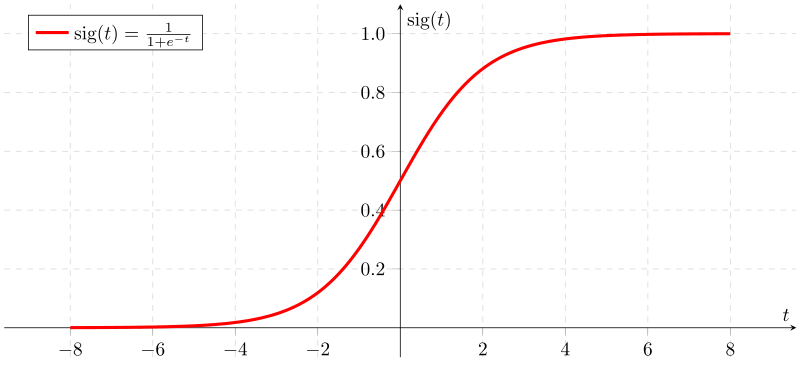
\includegraphics[width=1\textwidth]{pictures/Sigmoid-function}
 \caption{A Sigmoid curve otherwise known as an S-curve is defined by the formula $S(x) = \frac{1}{1 + e^{-x}} = \frac{e^{x}}{e^{x} + 1}$.}
 \label{fig:scurve}
\end{figure}

On an S-curve (see \autoref{fig:scurve}) or a bell curve, the beginning of the slope looks a lot like an exponential curve. In systems dynamics, an exponential curve shows self-reinforcement, i.e., a positive feedback curve without limits. Maybe this is what excites Singulatarians --- and scares systems people. Most people outside the Singularity bubble believe in S-curves, namely that nature adapts and self-regulates and that even pandemics will run their course. Pandemics may cause an extinction event, but growth will slow and humanity and society will adapt. But the notion of Singularity --- especially as some sort of savior  that will allow us to transcend the messy, mortal suffering of our human existence --- is fundamentally a flawed one.

This sort of reductionist thinking isn't new. When B. F. Skinner discovered the principle of reinforcement and was able to describe it \cite{skinner1938behavior}, we designed education around his theories. Scientists of learning know now that behaviorist approaches such as Skinner's only work for a narrow range of learning, yet many schools continue to rely on drill and practice. Take as another example the eugenics movement, which greatly and incorrectly over-simplified the role of genetics in society. This movement helped fuel the Nazi genocide by providing a reductionist scientific view that we could ``fix humanity'' by manually pushing natural selection. The echoes of the horrors of eugenics exist today, rendering almost any research effort to link genetics with things like intelligence taboo.

We should learn from our history of applying over-reductionist science to society and try, as Wiener says, to ``cease to kiss the whip that lashes us.'' While it is one of the key drivers of science --- to elegantly explain the complex and reduce confusion to understanding --- we must also remember what Albert Einstein said: ``It can scarcely be denied that the supreme goal of all theory is to make the irreducible basic elements as simple and as few as possible without having to surrender the adequate representation of a single datum of experience'' \cite{einstein1934method}. We need to embrace the unknowability --- the irreducibility --- of the real world that artists, biologists and those who work in the messy world of liberal arts and humanities are familiar with.

\subsection{Changing the Goals of a System}

\label{sec:meadows}

Donella Meadows described not only how systems worked, but how to intervene in these systems \cite{meadows_leverage}. By adjusting flows, feedback, goals, rules, how things are connected, etc., a system can be influenced and modified.

Meadows lists 12 ways to intervene in a system and lists them in reverse order of effectiveness.

\begin{quote}
\textbf{Places to intervene in a system according to Meadows}
(in increasing order of effectiveness)

\begin{etaremune} % downcounting enumerate
\item Constants, parameters, numbers (such as subsidies, taxes, standards).
\item The sizes of buffers and other stabilizing stocks, relative to their flows.
\item The structure of material stocks and flows (such as transport networks, population age structures).
\item The lengths of delays, relative to the rate of system change.
\item The strength of negative feedback loops, relative to the impacts they are trying to correct against.
\item The gain around driving positive feedback loops.
\item The structure of information flows (who does and does not have access to information).
\item The rules of the system (such as incentives, punishments, constraints).
\item The power to add, change, evolve, or self-organize system structure.
\item The goals of the system.
\item The mindset or paradigm out of which the system --- its goals, structure, rules, delays, parameters --- arises.
\item The power to transcend paradigms.
\end{etaremune}
\end{quote}

\begin{figure}[h]
 \centering
 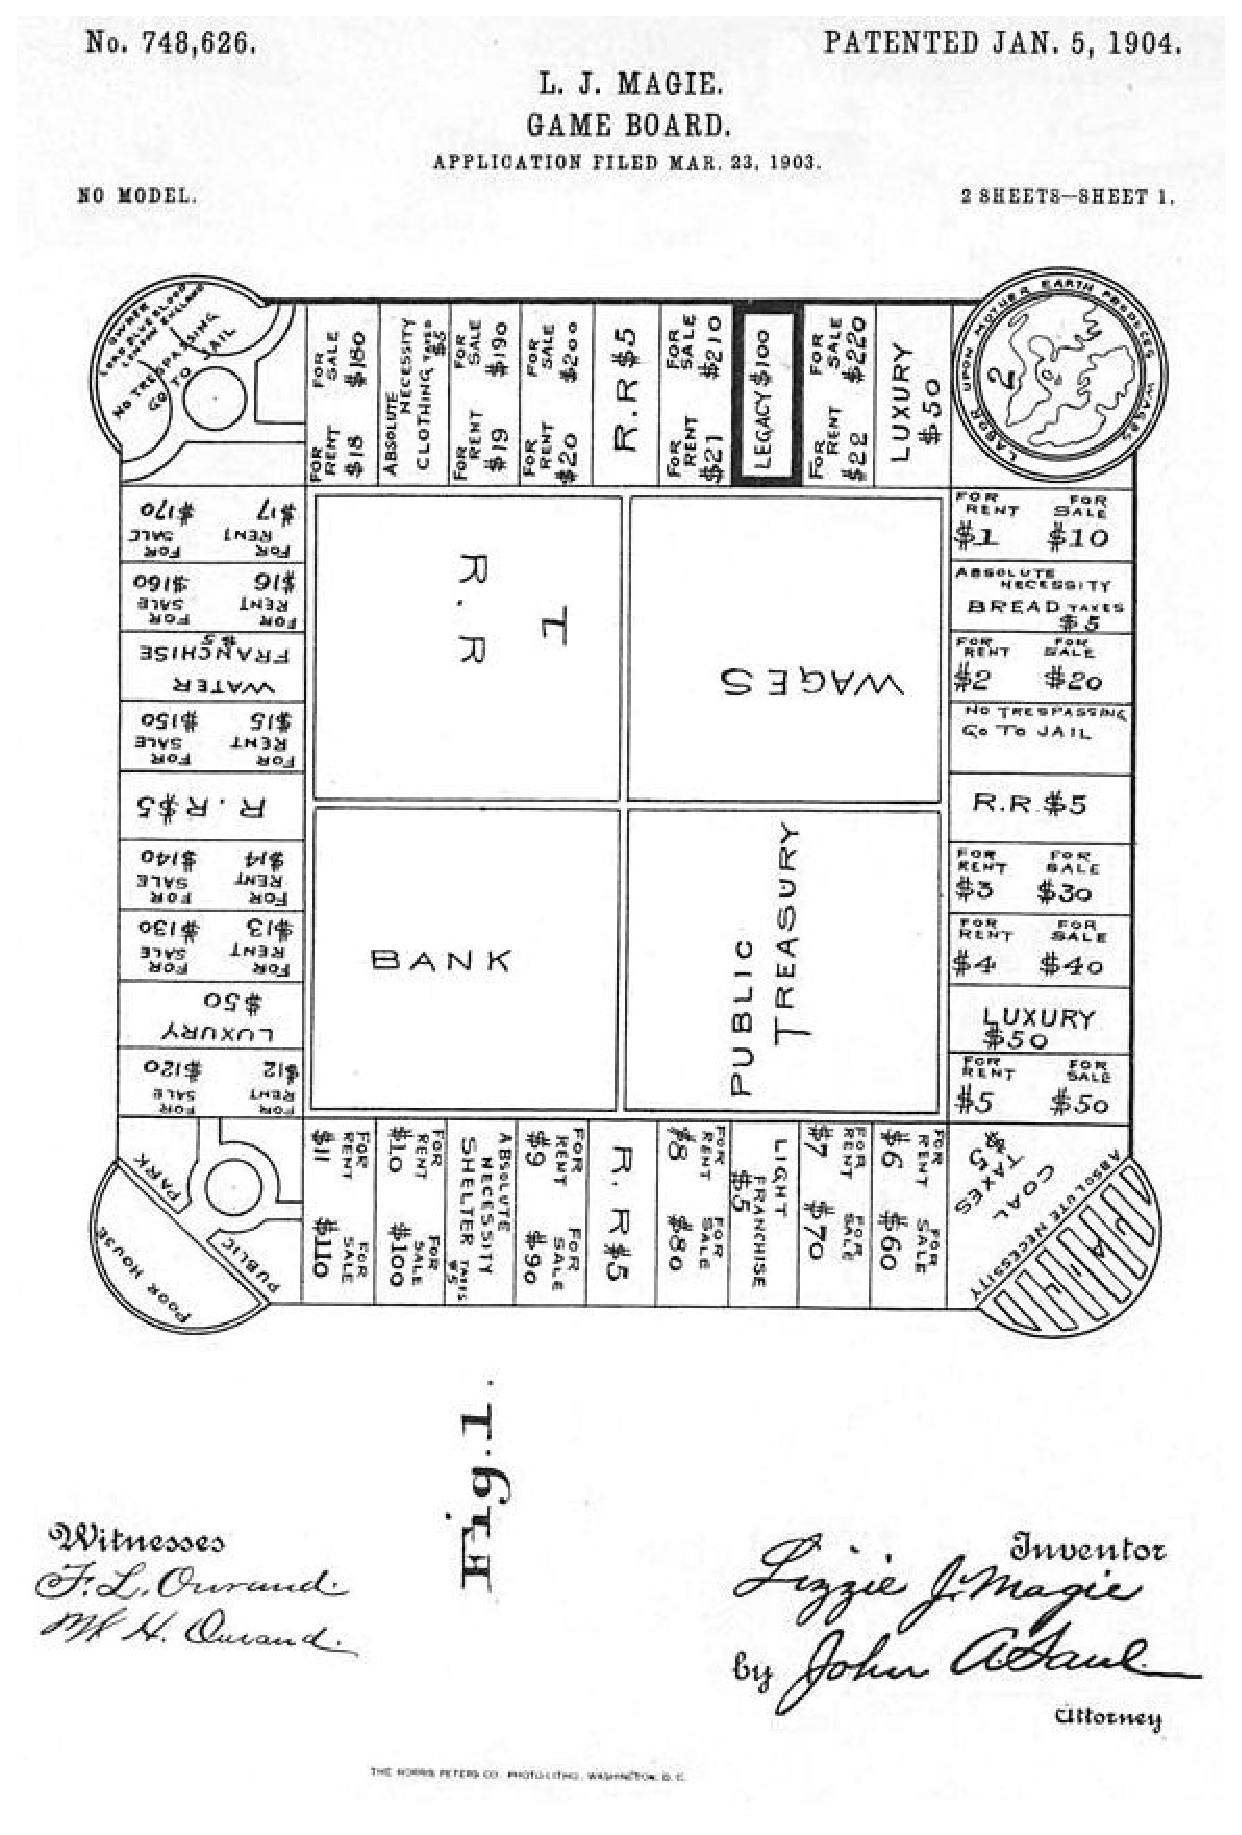
\includegraphics[width=.5\textwidth]{pictures/landlords-game.eps}
 \caption{The first patent drawing for Lizzie Magie's board game, \emph{The Landlord's Game}, dated January 5, 1904}
 \label{fig:landlords-game}
\end{figure}

The story of the game of monopoly provides a strong example of how these layers relate and why Meadows says the paradigm as the strongest driver of change in a system. Everyone knows the traditional Parker Brothers game of \emph{Monopoly}. What many people don't know is that \emph{Monopoly} \cite{monopoly} is based on a 1902 game called \emph{The Landlord's Game} \cite{landlords-game}, patented in 1904 by Elizabeth Magie (see \autoref{fig:landlords-game}). Magie's game was based on the economic principles of Georgism, which advocated a single tax on unimproved land, and the game was designed to show how rents enrich property owners and destroy tenants. Magie hoped that kids would play the game and learn about the unfairness of the capitalist system. The Parker Brothers version of the game didn't substantially change the rules --- it just changed the goal. Instead of aiming to teach children about the unfairness of capitalism, the goal of Monopoly was to become the capitalist and bankrupt all your friends. The thing to note here is that nothing in Meadows's list from 12-4 changed. Only the goal changed. As we think about how to ``fix'' the climate problem, by understanding that maybe somehow the goal --- to grow and eliminate the competition --- could change, maybe we don't need to change so many of the other layers. On the other hand, it might also show that even if we change a lot of the parameters and even the rules, unless we change the goal, we won't change much.

The goals are number three on the Meadows list. Number two is the paradigm --- in this case the paradigm of capitalism --- that drives the goal of what it means to win at the Parker Brothers version. The number one place to intervene is the power to transcend paradigms --- culture changes and paradigm shifts.

Goals and behavior are hard to change. We often believe that if we just labeled food better or if we could just make a convincing argument that our behavior negatively impacts the health of the planet, people would behave differently. But for many people, it's not an information problem. The Heart Attack Grill \cite{heart-attack} in Las Vegas serves Triple Bypass Burgers that have 9,982 calories and even Coronary Dogs. The waitresses are dressed as nurses and you eat for free if you weigh over 350 pounds. (see \cref{fig:heart-attack}) You often have to wait in line to get in, and several people have had heart attacks while eating there. In the case of the Heart Attack Grill, it's clearly not an information problem --- it's a culture, story and style problem.

\begin{figure}[h]
 \centering
 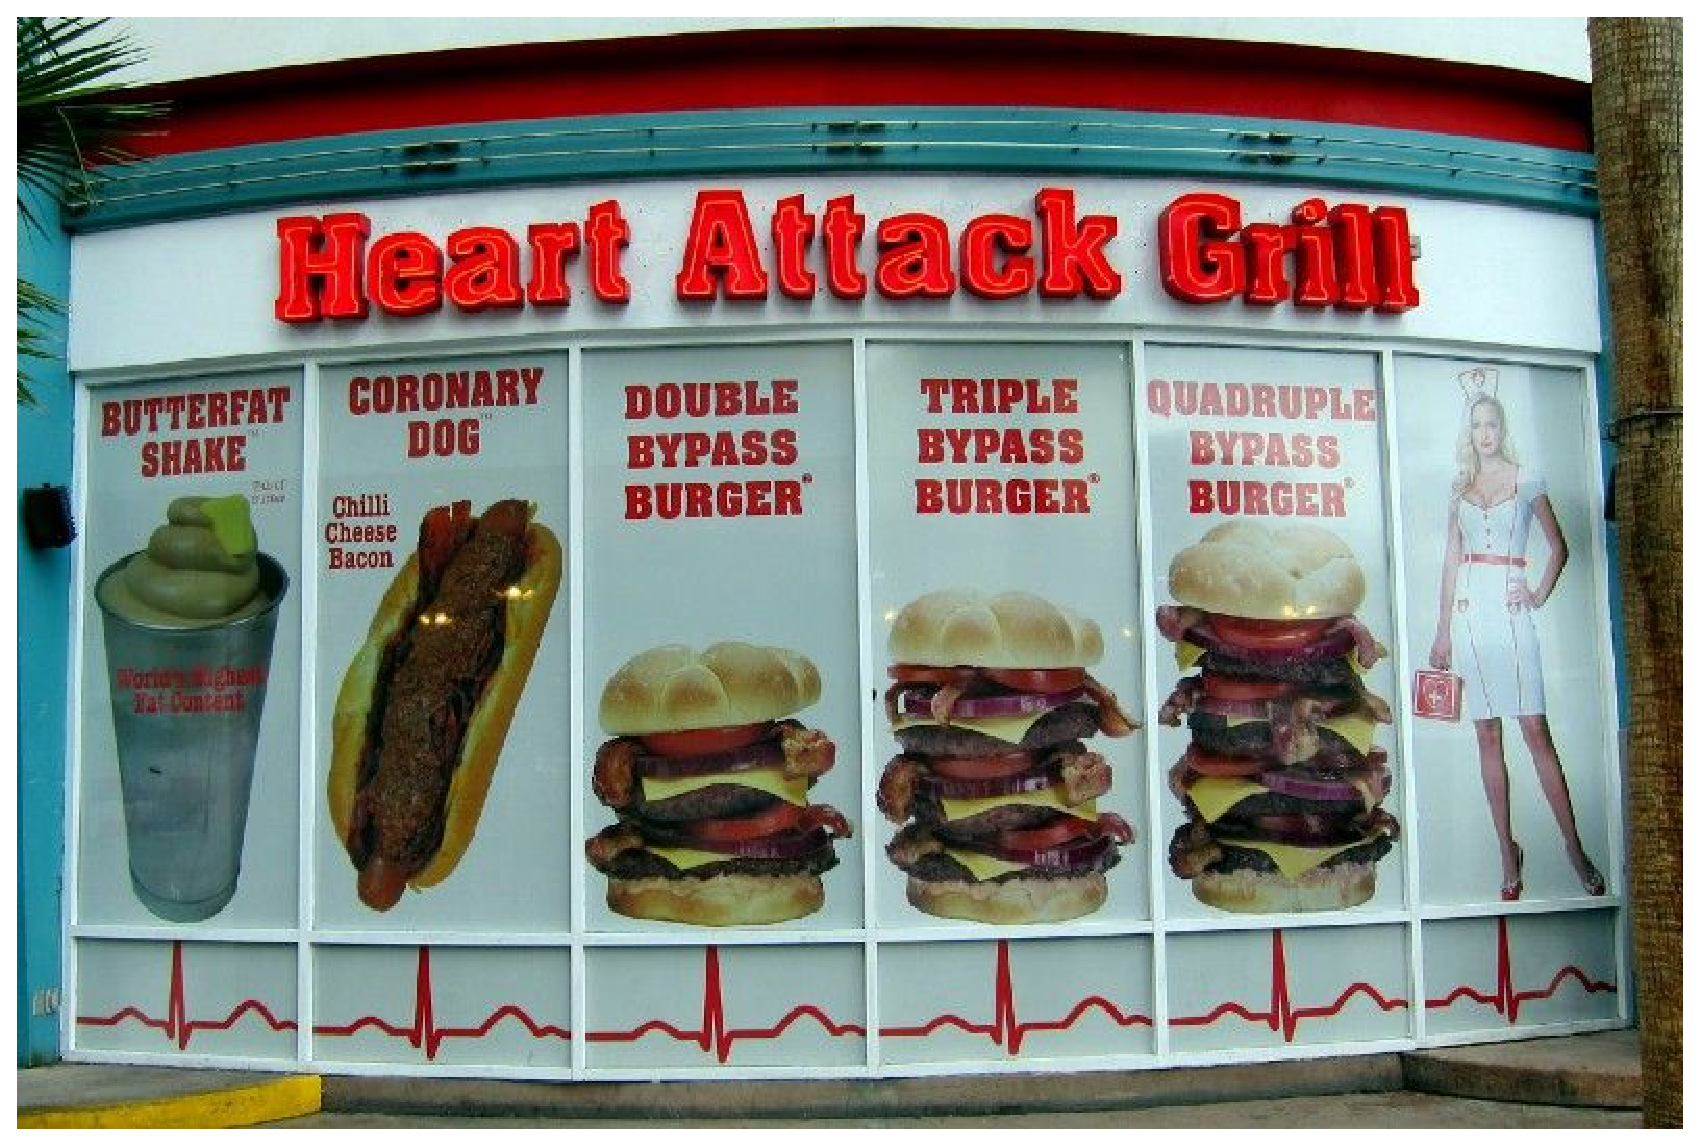
\includegraphics[width=.5\textwidth]{pictures/heart-attack.eps}
 \caption{Heart Attack Grill}
 \label{fig:heart-attack}
\end{figure}


In 2008, Canadian health workers on assignment in Cambodia were trying to solve a health problem caused by a lack of iron in the diet of Cambodians. The workers tried handing out supplements and educating people about the need for iron, but none of that worked. They happened to hear a local story about a ``good luck'' fish. So they fashioned a fish out of iron that Cambodians could throw in their pots when they were cooking. The ``lucky iron fish'' was a huge success, delivering a significant positive health outcome \cite{charles2010iron}.

\subsection{Interventions through Arts}

Health workers are not the only people who try to modify behavior through cultural intervention. During the Cold War, the \ac{CIA} used modern art as a ``weapon'' to combat communism \cite{cia-communism}. The spy agency promoted modern art, which embodid the creativity and freedom that Russian art, tied as it was to communist ideology, lacked.

Intervening at the paradigm level of complex systems can be achieved by developing a sensibility appropriate to the environment and the time. These interventions are more like music than an algorithm. Music is about a sensibility or ``taste,'' with many elements coming together into a kind of emergent order. Instrumentation can nudge or cause the system to adapt or move in an unpredictable and unprogrammed manner, while still making sense and holding together. Using music itself as an intervention is not a new idea; in 1732, Andrew Fletcher (see \autoref{fig:fletcher}), a Scottish writer and politician, wrote, ``if a man were permitted to make all the ballads, he need not care who should make the laws of a nation'' \cite{brown2015eighteenth}.

\begin{figure}[h]
 \centering
 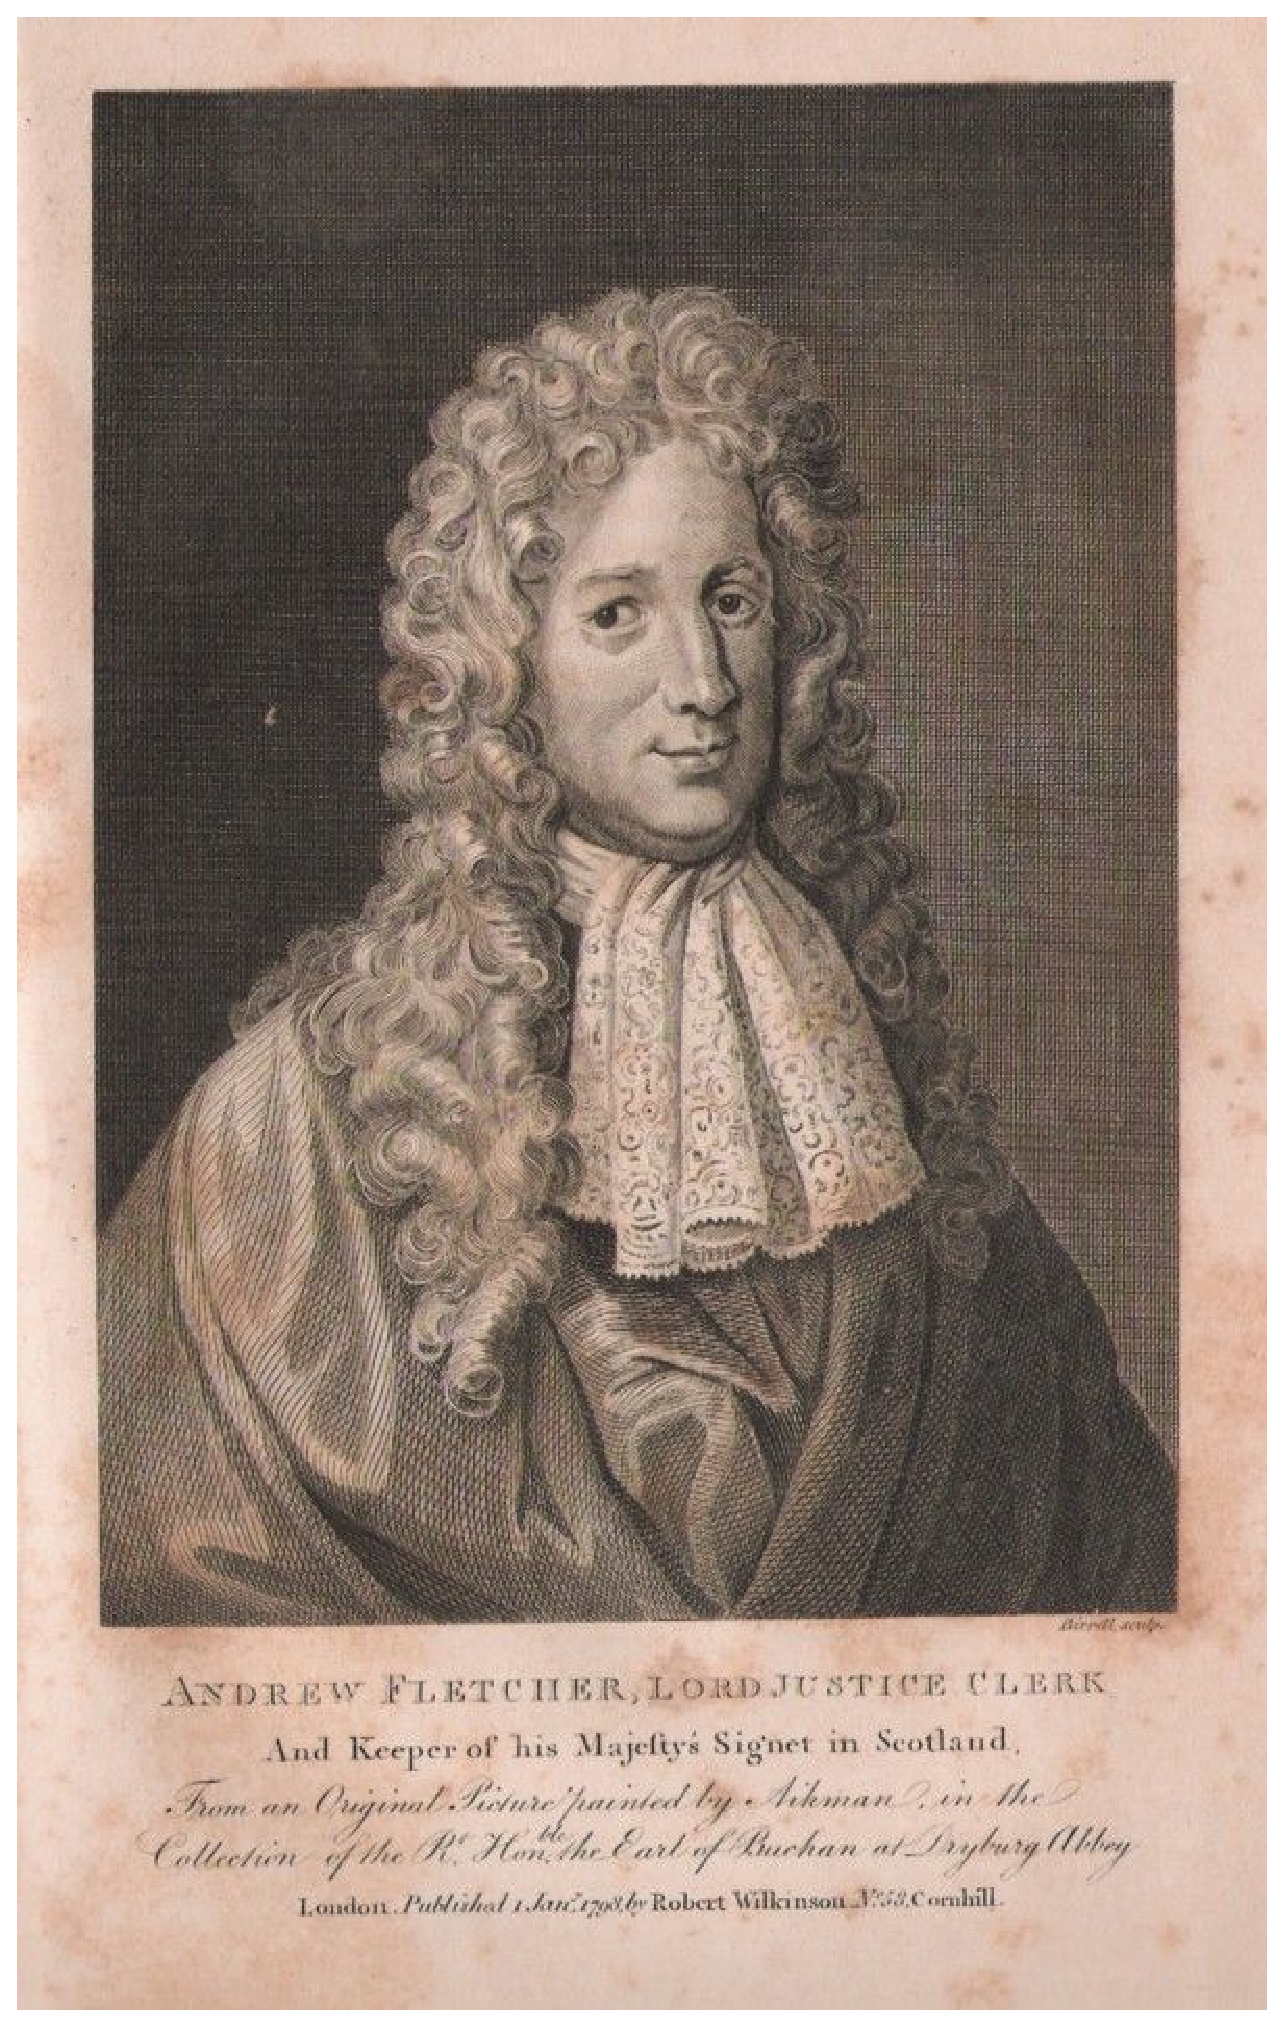
\includegraphics[width=.5\textwidth]{pictures/fletcher.eps}
 \caption{Andrew Fletcher of Saltoun (1655 -- September 1716)}
 \label{fig:fletcher}
\end{figure}

If writing songs instead of laws feels frivolous, remember that songs typically last longer than laws; have played key roles in various hard and soft revolutions,; and end up being transmitted person-to-person along with the values they carry. It's not about music or code. It's about trying to affect change by operating at the level songs do. This is articulated by Meadows, among others, in her book \textit{Thinking in Systems} \cite{meadows2008thinking}.

\subsection{A Culture of Flourishing}
\label{sec:cultureflourish}

Developing a sensibility and a culture of flourishing, and embracing diverse measures of ``success,'' depend less on the accumulation of power and resources and more on the variety and richness of experience. This is the paradigm shift that we need, and it will provide us with a wealth of technological and cultural patterns to draw from to create a highly adaptable society. This diversity also will allow elements of the system to feed each other without the exploitation and extraction ethos created by a monoculture with a single currency. It is likely that this new culture will spread as music, fashion and other forms of art as well as through spirituality.

As a native Japanese, I was heartened by a group of junior high school students I spoke to in Japan recently who, when challenged about what we should do about the environment, asked questions about the meaning of happiness and the role of humans in nature. I am likewise heartened to see many of my students at the MIT Media Lab and in the Principles of Awareness class that I co-teach with the Venerable Tenzin Priyadarshi using a variety of metrics (currencies) to measure their own success and determine meaning and grappling directly with the complexity of finding one's place in our complex world.

\marginpar{I think that it will yet again be about the music and the arts of the young people reflecting and amplifying a new sensibility: a turn away from greed to a world where ``more than enough is too much,'' and where we can flourish in harmony with Nature, rather than through control of it.}I'm also working with organizations such as the IEEE, which is designing guidelines for the development of artificial intelligence based on human wellbeing instead of simply around economic impact \cite{chatila2017ieee}. The work by Peter Seligman, Christopher Filardi, and Margarita Mora from Nia Tero \cite{NiaTero71:online} (described later in \autoref{sec:indigenous}) approaches conservation by supporting the flourishing of indigenous people, not undermining it. Another example is that of the Shinto priests at Ise Shrine, who have been planting and rebuilding the shrine every twenty years for the last 1,300 years, physically demonstrating the beauty and amazing capacity for renewal that we see in the cycle of nature.

In the 1960s and '70s, the hippie movement tried to pull together a ``whole earth'' movement, but then the world swung back toward the consumer and consumption culture of today. I hope and believe that a new awakening will happen and that a new sensibility will cause a nonlinear change in our behavior through a cultural transformation. While we can and should continue to work at every layer of the system to create a more resilient world, I believe the cultural layer is the layer with the most potential for a fundamental turn away from the self-destructive path that we are currently on. I think that it will yet again be about the music and the arts of the young people reflecting and amplifying a new sensibility: a turn away from greed to a world where ``more than enough is too much,'' and where we can flourish in harmony with Nature, rather than through control of it.


\subsection{Communities and Values}
\label{intro:communityvalues}

Meadows, in her essay ``Leverage Points'' \cite{meadows_leverage} about ``Places to Intervene in a System,'' explains that the most effective way to intervene in a complex system --- ``a corporation, an economy, a living body, a city, an ecosystem'' --- is with the power to transcend paradigms. That, she says, allows us to change ``The mindset or paradigm out of which the system --- its goals, structure, rules, delays, parameters --- arises.'' The goals determine the evolutionary direction as well as the direction of a system such as a community.

\marginpar{In ``Supercooperators: Altruism, evolution, and why we need each other to succeed'' \cite{nowak2011supercooperators} Nowak and Highfield describe the evolution of cooperation and mechanisms for cooperation. They argue that evolution is not only competition but also cooperation, and that cooperation is the master architect of complexity.}In ``Supercooperators: Altruism, evolution, and why we need each other to succeed'' \cite{nowak2011supercooperators} Nowak and Highfield describe the evolution of cooperation and mechanisms for cooperation. They argue that evolution is not only competition but also cooperation, and that cooperation is the master architect of complexity. In ``Spontaneous giving and calculated greed,'' researchers argue that people are intuitively cooperative and thus need to``calculate'' to overcome their cooperative impulse and become greedy \cite{rand2012spontaneous}. In ``Cooperating with the future'' \cite{hauser2014cooperating} the argument is that a large altruistic, majority would vote to cooperate with a longer view of the future in a democratic setting.


In Eric Raymond's 2001 classic, ``The Cathedral and the Bazaar: Musings on Linux and Open Source by an Accidental Revolutionary '' \cite{raymond_cathedral_2001} he describes traditional software development as the equivalent of a cathedral with top-down control and organization whereas open source software was more like a bazaar --- self-organizing and decentralized in nature. In ``Coase's Penguin, or, Linux and The Nature of the Firm'' \cite{benkler_coases_2002}, Yochai Benkler, a professor at the Harvard Law School, describes open source communities and introduces the notion of commons-based peer production. The firm, according to Ronald Coase, when he was a professor of economics at the University of Chicago Law School, increases productivity beyond gains that would take place simply in a free market by allowing the management of and the direction of resources in an organized way \cite{coase_nature_1937}. Benkler argues that the Internet has created  a way for participants in an open source project like Linux or Wikipedia to deploy their own labor to the tasks most suited to them without centralized management. He argues that because of lower costs and the decentralized nature of these systems, a community can be productive and create assets such as Linux and Wikipedia in the ``commons,''  outside of formal legal structures such as a firm or corporation.

The productivity of a community and what it produces is tied to how the community is designed and how well it is flourishing. Communities with productive outputs exist in many fields. For instance, communities of engineers work on open standards; communities of venture capitalists and entrepreneurs build startups in a startup ecosystem; communities of lawyers work on open source licenses; a community of developers work on Bitcoin; the community of members in a subculture like the hippie movement produced cultural products. It is the title of David Weinberger's 2002 book about the Internet, \textit{Small Pieces Loosely Joined} \cite{weinberger2008small}.

A flourishing community is very similar to a flourishing ecosystem with similar drivers, attributes and outputs. Turning back to Meadows' work on intervening in complex systems such as ecosystems, we can apply systems dynamics to communities as well.

As complex adaptive systems, communities can be resilient, they can collapse, they can grow, they can change. The values or paradigms of a community determine the aesthetic style of the output. The hippie movement embraced a world view that was natural, anti-establishment, psychedelic, loving and peaceful. Hippies wore tie-dye shirts, smiley face pins and long hair in solidarity with Native Americans, and their music was participatory and inclusive, producing musicians like the Grateful Dead. This sensibility also determined the evolutionary process that produced the movement's strategies and popular ideas, such as protests, communes and the emergence of the \emph{Whole Earth Catalog}.

The values of modern, neoliberal capitalism are fundamentally rooted in the paradigm of productivity and money, with almost everything measured in financial terms. Progress and growth of the economy are a kind of true north compass heading toward which everything is pointed, and it is against this payout that corporations, individuals and governments are measured and optimized. We have social services, culture, education and research, of course, but economic impact is the primary measure of their success and value. Established economists have questioned free market economics, from Economics Nobel Prize winner Elinor Ostrom's on sharing resources and governing the commons \cite{ostrom2015governing} to another Nobelist, Joseph Stiglitz, who criticizes free market fundamentalists and GDP as a reductionist measure of a healthy society \cite{stiglitz2010freefall}. However, their views have failed to sway the mainstream economic policies and behavior of society.

This has not necessarily been the case historically. Indigenous cultures such as Shinto, Maori, Native American, and just about any long-lasting historical community connected with nature typically have cultures based on flourishing together with nature and living in a vibrant but sustainable way. These values generate an internally coherent and rich culture with rituals, production and resilience that is nearly incomprehensible to those who live in capitalist, industrial cultures \cite{kohn2013forests}.

For instance, Shinto priests at Ise Shrine, as mentioned, have been planting and rebuilding the shrine every twenty years for the last 1300 years in a celebration of renewal and the cyclical quality of nature. The process involves many rituals, including fertilizing the mountains with oysters from the sea. For thousands of years, the shrine and its keepers have lived with and celebrated nature, not growing or ``improving'' but nonetheless flourishing. In fact, the seventh-century Emperor Tenmu banned livestock and meat, essentially establishing vegetarianism by fiat on an island that could not easily sustain a livestock-based food culture. Such values come from the nature-friendly, animist Shinto worldview \cite{zenjiro}. (Buddhist values also had a substantial influence.)

There have always been subcultures in society that have operated with alternative paradigms and goals. Some of these were different forms of governance with some of the same paradigms, such as communism with its  philosophy of managing resources and growing economies.

Other subcultures, such as hippies, developed new paradigms that transcended some of the basic paradigms of American society, with its worship of growth and the focus on property ownership. These movements and the communities that have supported them have played an essential role in the development of the Internet and positive social change, such as the civil rights movement. The next section will describe the role that the hippies and the Internet have played.

Many such sub-cultures and communities start through some sort of mind-expanding experience. Historically, these have come from contemplative practices that have driven religions like the Sufi, Gnostics, Yoga, Kabbalah and Buddhist meditation. These practices have often led to religious or spiritual movements that, at least at the beginning, seem to transcend the paradigms of the day, creating an alternative system, or sometimes co-existing, within traditional society --- church and state.

These cultures and subcultures are dynamic, merging, forking, dying, giving birth, cross-pollinating and so on. Some evolution in these communities is natural, but some of the change is a result of designers who have intervened in these systems by transcending paradigms, nudging values, making connections and otherwise perturbing these communities.

In \textit{Social Physics}, Alexander Pentland, a faculty member at the Media Lab, describes the use mathematical models and data science to understand the flow of ideas through systems and how people react to them \cite{pentland2015social}. Using these new tools, we may make headway in understanding the spread and impact of culture and new ideas.

Evolutionary dynamics show that individuals use mutation to try new strategies, competing with each other for the payout. The most successful strategies reproduce and disseminate themselves. A system of different individuals cooperating and competing with each other creates an ecosystem. We can model a community as a kind of ecosystem with a competition of ideas, strategies and tastes that are determined to be more ``fit'' based on how they measure against the values of the community --- the paradigm. By influencing the paradigm, the community's evolutionary dynamics can be influenced. These dynamics can increase robustness and allow a community to adapt to changes in the environment or its relationship to other communities and intersecting systems at other scales such as health, the environment, or the technological.

They key method of my theory of change is to shift the paradigms in all of the systems described in this chapter by intervening in communities to influence their values and culture. That way we can change the evolutionary game that the individuals and the system respond to, and fundamentally change the behavior of the system and its outputs, structure, and growth. In this section, I explore learnings and different ways that we can intervene in, manage, and harness the power of communities.

\subsection{How Nightclubs Work}

While I learned a great deal from online communities, my early experience in the nightclub scene helped to provide me with some insights into how culture manages communities and communities manage culture in a much more visceral way.

When I was attending the University of Chicago, I started exploring the nightclub scene in the city. It was in the late 1980s when \ac{AIDS} was taking a huge toll, especially in the gay community. My fellow students were all fairly similar, relatively privileged and focused mostly on completing their degrees and getting a job.

What I encountered in the nightclubs in Chicago was a diverse community of working-class people helping each other, loving, sharing, supporting, and creating very humane and sophisticated systems to flourish in a difficult environment.

The nightclubs were a community but also the hub of many of different communities. I started spending a lot of time in a community centered in the North Side of Chicago, around the Cabaret Metro and the Smart Bar. I occasionally worked as a DJ at the Smart Bar. (I had a more regular DJ job at another club called The Limelight, but the community around it wasn't as interesting to me.) I learned a lot at the nightclub, and one of my most important learnings was that elite people in society often underestimated the values, intelligence, and contributions of working-class people. I also learned a lot about participating in and managing diverse and generative communities. 

A key learning was that influence in one community didn't necessarily translate into influence in another. Being rich, smart or famous in the ``outside world'' didn't translate to influence many other communities. Indeed, an effort to try to translate that influence often had reverse effect. It was also clear that these communities all interacted and that the complex set of relationships, values, and measures of influence created an extremely complex and resilient network quite incomprehensible from the outside.

A DJ in a nightclub has the ability to influence a very important currency in the physical space --- the music. This way a key factor in the behavior of individuals as well as groups in the space and that significantly affected the financial and social success of a nightclub. By changing the music, you can move different groups of people onto the dance floor, to the bar, out of the club, or get groups to mix with each other. Different songs or genres are familiar to different cultures and communities. Some songs make people dance, some make them stop and get a drink and some make them leave.

\marginpar{ The DJ is just selecting the ``background music'' but might have the most power to shape the culture of a club.}In addition, a DJ over time can lead the community around the club in new directions by introducing new trends in the context of the trends that the members of the community already know. The DJ is just selecting the ``background music'' but might have the most power to shape the culture of a club.

I eventually dropped out of the University of Chicago to become a professional DJ for awhile. I later moved to Tokyo where I ran a nightclub for a year to try to understand the cultural differences. I often think of being a DJ as a metaphor for what I do at the Media Lab and in other communities that I am part of: I watch the behavior and dynamics of the community and intervene culturally through music or equivalent higher level sensibilities to try to tune the flourishing and the direction of the community. This cannot be accomplished without a deep understanding of the relationships of the different subcultures, their tastes and the experiences and values that drive those tastes.



\subsection{The Hippie Movement}

The hippie movement was a movement with music as a key component among a rich array of elements.

The history of the hippie movement is well documented and has a number of interwoven narratives. Most will trace its roots to the legal and academic, at least initially, to the study and use of psychedelic drugs such as LSD and psilocybin. These mind-expanding drugs created an ``awakening'' among young people during a very politically charged period in American history. As I mentioned in \autoref{sec:hippiesinternet}, 1967 was the year the Grateful Dead's first album debuted, as well as the Summer of Love and the Detroit Riots .

At the time, Timothy Leary was urging people to``Turn on, tune in, drop out.'' He would run for governor of California against Ronald Reagan under the banner ``Love for Gov,'' and the Beatles would write ``Come together'' as his campaign song. Hippies lived in communes and espoused liberal values that stood in a stark contrast to the conservatism of the generation before them.

They cared about the earth and native Americans. Stewart Brand, who was fighting for the protection of Native American values and trying to prevent the ``cowboyization'' of the Native Americans, wore his hair long in solidarity with them, which became a symbolic emblem of the hippies.

The hippies also built systems. Grateful Dead shows became moving communities, with families following the band around for its entire tour. The Dead allowed taping of their shows; people shared the tapes; parking lots became markets where those tapes were sold, and backstage was a daycare center for kids.

The hippie movement intersected with the Cybernetics movement, and many of the tool builders came together. Stewart Brand, Howard Rheingold and others created a new kind of publication in the Whole Earth Review, writing about new tools and techniques for the hippie do-it-yourself lifestyle. The same community that relied on the Whole Earth Review quickly created The Whole Earth 'Lectronic Link, or The WELL, a very early computer network to connect communities.

The general arc of the hippie movement is cannily similar to many religions. It began with mind expansion and, as in many traditional religions, with the enlightenment of a prophet and a sort of group contemplative practice during a difficult political period. This led to the formation and massive adoption of a new set of values that spread across a subculture. In some cases, as with Christianity and Islam, this pattern of development leads to an overthrow of the status quo, becoming the dominant culture, and in other cases, as with the hippie movement, it creates long lasting subcultures and institutions.

Many of these movements have arisen organically and spontaneously, but some have been designed.

\subsection{Hippies and the Internet}
\label{sec:hippiesinternet}

The culture that created the Internet and help set its trajectory was critical to its success. While there were many factors that contributed to the success of the development of the Internet, the hippie culture contributed both a cultural backdrop as well as a values framework that contributed to the development of the Internet.

I met Timothy Leary in the summer of 1990 in Tokyo, when I was running a night club there. Leary was a former psychology professor at Harvard University who conducted many of the early academic experiments with psychedelic drugs. He later became one of the leaders of the hippie and New Age movements. When I met Leary, he was interested in virtual reality and computer graphics. I introduced him to the Japanese youth scene in the '90s, and he introduced me to the San Francisco cyberpunk subculture. He later adopted me as a ``godson,'' and we attempted to write a book together and spent time discussing emerging communities in Japan and the US.

I met John Perry Barlow that same summer, when my mother moved to Los Angeles, and we were installing my sister in college at Stanford. Leary drove us from Los Angeles to San Francisco to introduce us to his community there. (He didn't have a driver's license.) He threw a party for us at the Mondo 2000 House to introduce us to his San Francisco crowd, and Barlow was there.
 
This was 1990 --- before \textit{Wired Magazine}, before the web. It was all about cyberpunk: leather jackets, CD-ROMs, weird drugs, raves, VR. South Park was a needle park, and there were raves around Toon Town. I remember raves advertising ``Free VR.'' Silicon Graphics computers were used to make amazing rave fliers that eventually inspired the design for \emph{Wired Magazine}. All that started in and around South Park and and was the genesis of the gentrification that transformed the neighborhood into what it is now: a chic neighborhood with fancy cafes and many well-known Internet startups.

\marginpar{Cyberpunk was a sort of punk rock-meets the hippies-meets computers, and the proximity to Haight-Ashbury, Silicon Valley, and Berkeley created the weird sub-culture where a lot of Internet stuff started.}Cyberpunk was a sort of punk rock-meets the hippies-meets computers, and the proximity to Haight-Ashbury, Silicon Valley, and Berkeley created the weird sub-culture where a lot of Internet stuff started.
 
Leary and Barlow both had an amazing sense of humor, optimism and hope. This wasn't the optimism of giddy investors during a bubble. Rather, it was the optimism and humor that I sense in the Dalai Lama and others who have become self-aware through meditation, mind-expanding drugs or whatever it is that brings you close to understanding true nature and reality. It's that peculiar zone where you see all of the suffering, the injustice and just how messed up the world can be --- and you face this challenge with a fundamental confidence in human beings and a sense of humor.

It was a period where the primary motivation for people to do things wasn't about the money, but was a combination of hedonistic fun and the pursuit of a spiritual path. It was also a time of rebellion, disobedience and mind-expansion.
 
Timothy Leary used to say, ``Question Authority and Think for Yourself.''
 
Barlow's manifesto, \emph{A Declaration of the Independence of Cyberspace} \cite{barlow1996declaration}, was a great example of that awareness so particular to that time. It was a rallying cry for a new generation, for us. I remember when we were starting out, it felt like if we could just connect everyone and give them a voice via this amazing thing called the Internet, we'd have peace, love and fairness.

Other parts of the hippie movement also influenced the initial trajectory of the Internet. The WELL, one of the earliest online communities, directly followed from \emph{The Whole Earth Catalog} \cite{brand1981whole} and a community led by Stewart Brand and Howard Rheingold.

John Gilmore, a co-founder of the Electronic Frontier Foundation and the fifth employee of SUN Microsystems, created one of the earliest Internet service providers and called it The Little Garden. John was an activist with '60s values and continues to be an important part of the community.
 
Today, our dream of the world that Barlow wrote about seems like a distant dream, and Barlow himself was aware that this dream that held so much promise, the Internet or cyberspace, had fallen well-short of what he envisioned. ``My belief in the virtues of giving all humanity a voice did not take into account what would happen if you gave every one of a billion people his own virtual soapbox and street corner. Everybody's talking and nobody's listening,'' he said.

But he also said of his manifesto, ``I'm not sorry I wrote it. One day, I still believe, it will seem true.''
 
We're having to climb some mountains and suffer some bad weather. It almost feels like the winter of 1846 for the Donner Party \cite{stewart1960ordeal}. But Barlow gave us a compass heading --- bearings for our ultimate goal --- and I believe, as Barlow did, that one day it will seem true. 

But to make it true will require organizing, action and tenacity. We are in the darkest moments in global and American history that I remember.
 
I was born in 1966. I don't remember 1967 because I was just a year old. But in 1967, we had the Detroit Street Riots, which some called a rebellion. (I guess if you quash it, you get to name it). It was the worst incident of its kind in US history: 43 people  killed and 1,400 buildings burned to the ground before the National Guard put a stop to it. It was also the year that The Grateful Dead's debut album came out, and Barlow introduced the band to Timothy Leary at the Hitchcock Estate in Millbrook, New York. 1967 was also the year of the Summer of Love that kicked off the hippie movement. The hippies and the Grateful Dead opposed the Vietnam war and racism  with songs, love and humor.

\subsection{Movements}

The hippies created a movement, and while there was a group of core designers who came up with ideas, rallied people and resources, and led the movement, there was no organized plan. Rather, the community evolved, and did so in an environment where the clash of existing paradigms enabled the emergence of a new paradigm while dis-empowering the old.

There were other movements. The Punk Rock movement took hold after the hippie movement, and in a different way. It was more ``designed'' by Malcolm McLaren and Vivian Westwood, who founded bands like the Sex Pistols during the ``No Future Generation'' of the UK. They designed the fashion and the story, creating a subculture that would stun and sweep the world \cite{marcus2009lipstick}.

Punk Rock was more nihilistic and violent than the hippie movement and ended up becoming more commercial in many ways. However, it is important to note that fashion and music were essential to both of these movements.

For millennials, the hippies are a long gone movement that their grandparents were into. However, I believe that the hippie movement had a lasting impact on the values of the United States and the rest of the world. I also believe that we can learn from the successes and failures of the hippie movement as we participate and design the new movements today.
 
The collective movement for better gun control inspired by the kids from Parkland, Fla., and the \#metoo and TimesUp movements are among the most powerful of the day. The TimesUp movement is headed to overturn centuries of patriarchal power, while the teenagers are standing up against one of the most powerful political lobbies in the United States. There is another wave coming. It feels different from the hippie movement, but it feels like we're once again following the compass heading John Perry Barlow gave us to overthrow established and ossified power structures and, more importantly, the paradigms that feed them. There is a feeling of rebellion and revolution in the air. 

These movements have been sparked by anger and have used social media as a tool for organizing. They have a fundamentally different structure than the hippie and punk rock movements and are less a creation of a subculture and more about rebellion or uprising, similar to the civil rights movement or the Detroit Riots.

These movements have the successful, active management and development of communities in common, but the Internet and social media have fundamentally changed the dynamics --- in some ways for the better and some ways making things more difficult, as we will explore.
 % Chapter 3 - theory of change
\chapter{Practice of Change}
\label{chap:practice}

\textit{In theory there is no difference between theory and practice...} - Benjamin Brewster \cite{brewster1882} \\


The Media Lab has deep roots in Constructionism --- learning through doing --- beginning with Media Lab co-founding faculty member Seymour Papert who defined constructionism in his 1987 National Science Foundation proposal,``Constructionism: A New Opportunity for Elementary Science Education'' \cite{papert1986constructionism}. It is fitting that almost everything that I have learned, I have learned through doing things and being mentored along the way. This chapter represents three decades of learning through doing.

I have learned by experience that learning through doing can be hard at first, especially if you have very little learning before you start, for you may lack the frameworks that traditional educational models explicitly convey. What you learn by doing depends on what you happen to be doing, and so may lack the coherence that traditional discipline-based systems provide. It can be difficult to build that coherent view, and it's easy to go wrong if you don't know the extent of what you don't know: a lack of discipline and an absence of disciplines can lead to attempts to ``boil the ocean'' in pursuit of a single unified theory of everything.

However, over the years one's model of the world may start to come together, as one's influence and trust in many different networks mature; as one's ability to translate and connect ideas across networks and disciplines increases; and as opportunities and problems present themselves from odd but often useful perspectives.

My seven years as the Media Lab's director have put my natural affinity for constructionism to the test, for now I was expected to lead one of the most highly respected research centers in the world. But most academic institutions are not particularly comfortable with ``learning by doing'' or the community-based, antidisciplinary approach I have long advocated. In order to provide such an environment at relative scale --- about eight hundred people in our extended community --- required learning how to hop back and forth across the boundary that separates traditional institutional mechanisms and the ``heterotopia'' that has made the Lab so highly regarded externally, and so cherished by MIT and its community members. 

In this chapter we will explore this boundary.

\section{The Antidisciplinary Approach}
\label{antidisciplinaryapproach}

\marginpar{Being antidisciplinary faces the the same challenges that I did growing up: how do you manage being interested in learning about everything without the structure and the boundaries traditionally imposed? For both individuals and organizations, the best approach is passion-based constructionism.}An antidisciplinary approach is necessary to advance the paradigm shift that we require. The Media Lab is both the institute where the concept arose and the best example I know of an antidisciplinary organization.\footnote{Portions of the following sections about the Media Lab are based on a journal article and a talk that I gave at the Innovation Research Interchange induction ceremony in 2017, when I was the recipient of the IRI Medal. The talk was later published in the journal, \textit{Research-Technology Management} \cite{ito2017antidisciplinary}. It describes how the Media Lab works and provides my opinion about its trajectory and principles.}

Being antidisciplinary faces the the same challenges that I did growing up: how do you manage being interested in learning about everything without the structure and the boundaries traditionally imposed? For both individuals and organizations, the best approach is passion-based constructionism.

\subsection{Joining the Media Lab}

When I joined the Media Lab as its director in 2011, I had one way of doing things, and the Media Lab had another. 

I was transitioning from the world of Internet entrepreneurship and open-source governance to academia. At first, it didn't make sense that I, with my background as a scrappy entrepreneur, could fit in at a huge academic institution like MIT. But the Media Lab was different. It is antidisciplinary --- not opposed to disciplines, but explicitly seeking out ideas and research agendas that work across disciplines. The Media Lab has always favored research that falls into the white space between disciplines. It allows students and researchers the freedom to explore --- and to fail. And it has produced some groundbreaking inventions that its corporate members have gone on to commercialize with great success. Those differences, provide important lessons for all kinds of organizations --- research labs, companies, even academic institutions --- that are being challenged to adapt to the tidal waves of change that we're all facing now. 

\subsection{The History of the MIT Media Lab}

The Media Lab is somewhat peculiar, even for a highly diversified university like MIT. That peculiarity arises from the Lab's history. It was founded 32 years ago by former MIT president Jerome Wiesner and a young faculty member named Nicholas Negroponte. Wiesner had stepped down as president several years earlier but wanted to continue working in areas about which he was passionate, which included bringing the arts and sciences together at MIT. Negroponte, who was promoting a vision of a digital future that included a CAD system on everyone's desktop, was working on computer-aided design in the Architecture Machine Group in MIT's School of Architecture and Planning. Together they created the Media Lab.

And when they created it, they did something you can only do when your partner is the former president of MIT: They broke a bunch of rules. Typically in universities, you have labs and you have academic programs, and they tend to work like church and state in a healthy or unhealthy balance. The academic program offers classes to students and grants degrees. Labs, on the other hand, focus on raising funds to conduct specific research aimed at real-world impact. The Media Lab is both. It has its own academic program --- the Program in Media Arts within MIT's School of Architecture and Planning --- and it is also a research lab. 

The other unique aspect of the Media Lab is its funding model. When the Lab opened, approximately 80 percent of MIT's funding came from government sources and 20 percent came from private sources. The Media Lab was the exact opposite, with 80 percent of its money coming from corporate sources. This was partly a result of Wiesner's history. As science advisor to John F. Kennedy, he was sent to Japan to help that country rebuild its technology and research infrastructure. As a result, many in the Japanese business world felt a real debt to Wiesner. At the time Wiesner and Negroponte were planning the Media Lab, these companies had money to spend. So much of the money for launching the Media Lab came from the CEOs and chairmen of Japanese electronics firms. In fact, the Media Lab was even criticized for selling secrets to the Japanese \cite{MITDealW66:online}.

The way the lab handles its corporate support is also atypical for academia. Funds from corporate members do not support directed research, but rather go into one Lab-wide fund, and any IP (intellectual property) resulting from Lab research is available to be shared among all the corporate members. In the past, members could choose among different consortia to join based on their research interests, but today there is just one consortium for all members.

Currently, the total lab budget is about \$75 million, the majority from the consortium and some from government and other non-IP-generating research grants. As director, I distribute consortium funds to 25 research groups, which are working on everything from synthetic neurobiology to the future of opera. Each research group is made up of students and faculty members. Crucially, the research groups have almost full license to spend the money on whatever they want, at their discretion. This enables them to explore, fail, learn, and explore some more.

\subsection{How the Media Lab Works}

This structure has a couple of major consequences for the way the Media Lab works. 

First, it helps to create a strong sense of community. In a typical lab, if you're a faculty researcher, you write a grant proposal, your students work with you,and together you deliver the required results. Such a system makes it difficult for people from different labs or departments to work with one another. It can even make it difficult for the funding companies to work with one another. Everybody's working on their own grants, and the IP generated by that research must be protected from all the other groups. But at the Media Lab, the consortium owns the IP, so there's no barrier to collaboration. Twice a year, hundreds of people from our member organizations --- from LEGO to Lockheed Martin to governments --- come to the lab to learn about the current research. Amazingly, even companies that are normally fierce competitors, such as LG, Samsung, Toshiba, and Google, join together in this unique member community.

The pooling of IP gives us the freedom to fund things that others wouldn't. The member companies aren't supporting us so that we'll help them do better what they're already doing. They support us because we might do something they would never have thought to do on their own. That makes working in the white spaces core to the Media Lab's ``business model.''

We try very hard to find interesting areas of research that would be impossible to fund in other departments or labs because they are in between disciplines or are too risky and strange. In fact, we try to exit areas when they become mainstream.

\subsection{Accounting}

When I joined the Media Lab, it was recovering from the 2008 downturn in the economy. What I didn't know was that the Lab had during the 2001 downtown also suffered from a serious accounting error that had led to an overestimation of its financial resources: MIT and the Media Lab had been recognizing all revenue for a three year contract in the year the contract was signed, even when payment was not yet due. This made it look like the Lab had much more money than it really did. Because new contracts kept coming in, no one noticed until the downturn. Once the downturn hit it became clear that the Lab had been spending well ahead of revenue. In late 2001, this led to significant layoffs. 

While all this took place many years before I arrived, the Lab was still traumatized by this event, and across MIT still had a reputation for being poorly managed.

When I joined, I was told that the books were balanced and that the debt had been paid off. After my first year when the surplus from that year's income disappeared, I investigated and discovered that there was a hidden liability of millions of dollars somewhere in the accounting system of MIT.

After substantial effort in trying to fix the finances and accounting system, I reached out to a colleague of mine from several previous companies where we worked together. Barak Berkowitz had been the president of Six Apart and OmniSky, a public company, and had been an investment manager with me. He came in to help me fix the accounting system.

We discovered that the accounting system was set up in a way that made our finances completely opaque to both the Media Lab and central MIT finance. There was no consistent way to track the most basic things. How much money does the Lab have available to spend? How much money do we need next year? Did we make or lose money last year? The new Vice President of Finance, Israel Ruiz, had come from industry and understood how complicated and broken the accounting system was.

We spent many months trying to sort through what was actually going on in the accounting system. At the same time, we redesigned the financial reports to look more like a company with a balance sheet and a profit and loss statement. Originally, the Lab was set up as if it were a single research project that had been going on for thirty years and had no prospect of ending. Instead of the central MIT administration and the Media trying to hide things from each other, we made our system as transparent and representative of the facts as we could, and we agreed on a consistent way to judge the financial condition of the Lab.

We never were able to get to the bottom of the obscure liabilities that the Media Lab was thought to have with the central finance department so we agreed to start fresh, and zero the accounts from the day I took the job at the Media Lab.

Once the accounting system was fixed, we were able to build many systems, thanks to Berkowitz, the finance team, the human resources team, and all of the staff. From an operations perspective, the Media Lab was now running as much like a business as possible at MIT.

For the Media Lab to be both the instrument of change and an example of the theory of change it espouses, some very traditional structures need to be in place. Disruption needs a firm platform to stand on.

\subsection{Membership Model and Growth}

One of the first things that I did when I joined the Media Lab was change the label for our funders from ``sponsors'' to ``members''. I wanted to make it clear that the companies were members of our community and to be respected as colleagues, not our bosses telling us what to do or ``dumb money'' that stands back from community. While the Media Lab was never as directed as most labs, my predecessor, Frank Moss, appeared to be focused a bit more on commercialization to support the Consortium's member companies, which could have an inhibiting effect on the freedom that the Lab originally had enjoyed \cite{FrankMos10:online}. This was in part a response to the difficult financial situation that the Lab was in at the time after the 2008 downturn. I tried to make it clear that while we worked with our companies and listened to them, the Lab was exploring areas that the companies don't yet know they would be interested in.

I also initiated a price increase because the Consortium membership, \$200,000 a year, had not been increased for fifteen years. We decided to increase it to \$250,000 a year. Our initial presentation of this change was poorly communicated and we had significant pushback from companies. We got together, regrouped, tweaked the contract and reintroduced the change with much greater success. 

While this process damaged our relationship with some members and we lost a significant number of them, it turned out to be critical for building a tighter relationship with the companies that stayed. In addition the companies that left were the ones that did not believe they were getting value they wanted out of the Lab. We quickly replaced them with companies that were excited and more engaged with the Lab. This is consistent with the Lab's model of treating funders as engaged members of a unique research community. Today the average member spends well over \$300k a year with the Lab when you include incremental funding they provide to projects that especially interest them.

The consortium model described in the paper \autoref{antidisciplinaryapproach} has continued to thrive. The continuing robustness of the financial markets clearly have had a supporting effect, but our membership numbers and overall revenue has increased every year over the seven years that I've been here. (See \autoref{mlpandl}.)

\begin{figure}[h]
 \centering
 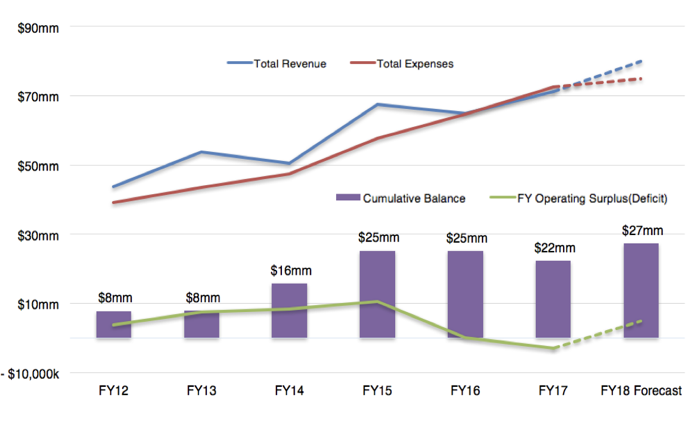
\includegraphics[width=1\textwidth]{pictures/mlpandl.png}
 \caption{Media Lab Consolidated P\&L}
 \label{mlpandl}
\end{figure}

Recently, we presented these numbers at a meeting of entire Lab. I reported that we had 475 full time staff including the students, and nearly 800 people in our ecosystem if we include the part-time undergraduate researchers in addition to the Masters and Ph.D. students. I reported these numbers with pride.

Later that evening when I was leaving the Lab, a long-time researcher who has a very good sensibility about the Media Lab culture approached me and asked, ``When are we too big?'' I mentioned that we had thirty tenure track slots and that we currently had 26 groups and that maybe that was a good limit. As I said that, I realized that some groups had become quite large. The researcher also mentioned that it is virtually impossible to know eight hundred people's names, much less to know those people well.

\marginpar{One significant question for me is, ``What is the right size for the Media Lab?'' How do we decide what to do and what not to do? How do we increase quality over quantity? How do we determine quality?}I realized that while I espouse the limits of growth and warn about the danger of focusing on growth, I had been doing it myself. Initially, fixing the accounting system and bringing in cash was essential to build up the health of the organization. But now we were healthy. Maybe more than enough is too much.

One significant question for me is, ``What is the right size for the Media Lab?'' How do we decide what to do and what not to do? How do we increase quality over quantity? How do we determine quality?

While some believe in a somewhat hierarchical model of tenure track faculty deciding everything, I believe that the dynamics of the community determine the quality and the flourishing of the system.

We were, in fact, facing one of the core dilemmas in the age of connected technology: How to scale community?

\subsection{Community}

When I arrived at the Media Lab, women had represented about twenty percent of the student population for as far back as we could see. The Visiting Committee, an external committee of a variety of experts from inside and outside of MIT that audits the Media Lab's overall performance every two years, had noted for the last four years that this gender diversity was unacceptable. Additionally, the number of minorities at the Media Lab was also unacceptable.

I had heard from former Media Lab graduates that they didn't recommend the Media Lab to prospective female applicants because it didn't feel safe for women. I realized that this wasn't an issue of just trying to get our faculty to admit more women -- they were in fact admitted in line with the percentage of female applicants. I realized that  to change the pipeline we needed not just to alter our communications about our culture, but change the reality of our culture, and of our community. While disciplines are based around topics, communities and cultures are based on the actual people in them.

I spent several years trying harder, but the numbers only moved slightly. Then we hired Monica Orta as a director of diversity. Her sole focus was on increasing the diversity of students applying to the Media Lab. But her first task was to actually make the Media Lab safer and more welcoming to minorities and women. We worked together to address issues as quickly as we could. For example, unacceptable behavior on mailing lists was immediately dealt with. Harassment and other issues were dealt with quickly and firmly. After some member company visitors talked to students in gender and racially insensitive ways, I opened the next member meeting with a message to the thousand attendees that they are members of our community, and we have zero tolerance for any member who does not support our community's values.

With Monica's help, now nearly fifty percent of incoming students are women. 

\begin{figure}[h]
 \centering
 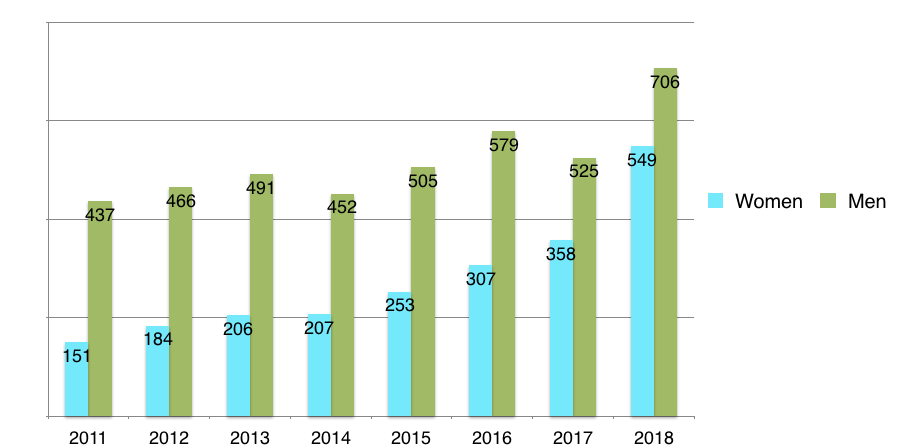
\includegraphics[width=1\textwidth]{pictures/mlgender.png}
 \caption{Master’s Applications by Gender}
 \label{mlgender}
\end{figure}

Unfortunately, our racial and ethic diversity has not improved as much as the gender diversity, but it is improving slightly. (See \autoref{mldiversity}.)

Our most recent faculty hire, Danielle Wood, is an African-American woman who has publicly vowed to make diversity an important part of her work.

\begin{figure}[h]
 \centering
 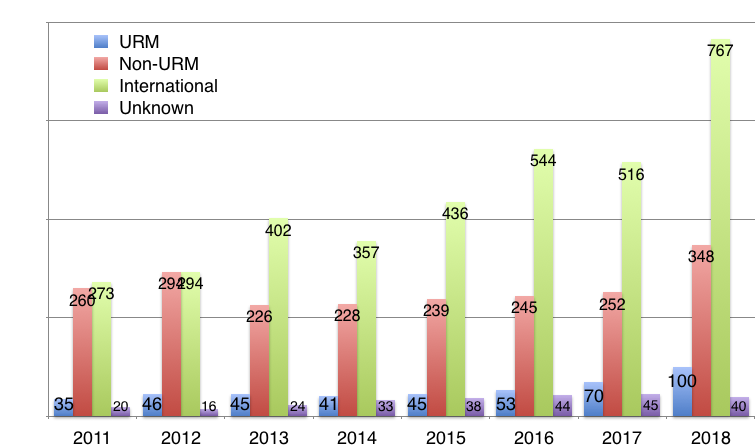
\includegraphics[width=1\textwidth]{pictures/2018mldiversity.png}
 \caption{Master’s Applications by Race/Ethnicity}
 \label{mldiversity}
\end{figure}

Diversity among the faculty hires has been more difficult than with students. The faculty do not turn over as quickly and since we add them one at a time, it is harder to implement policy.

This is now one of my most important areas of focus.

The total student application numbers of students have increased significantly and our response to faculty searches is also strong. (See \autoref{mladmissions}.) This is encouraging news, but I do worry that as we become competitive and able to hire stronger students and faculty who have significant competing offers, we could lose the Salon des Refusés feeling that has so characterized the Media Lab.

\begin{figure}[h]
 \centering
 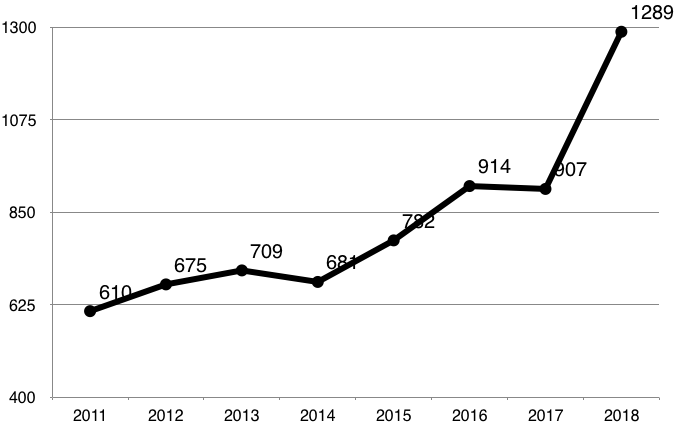
\includegraphics[width=1\textwidth]{pictures/2018mladmissions.png}
 \caption{Total Number of Applications (Master's and PhD)}
 \label{mladmissions}
\end{figure}

\subsection{The Media Lab Mindset}

The companies that interact with the Media Lab are seeking that discovery sensibility; they're looking for an exploration rather than a problem-solving kind of thinking. In a book I recently coauthored with Jeff Howe, \emph{Whiplash} \cite{ito2016whiplash}, I tried to capture the core principles driving the Media Lab. \emph{Whiplash} grew out of almost five years of discussion as my colleagues and I worked through the collision between the Media Lab's peculiar DNA and the DNA I brought from the Internet world. In those discussions, we developed a set of principles, iterated on over multiple faculty meetings, by asking two questions: What are the principles that define the Media Lab? and What are the principles that drive innovation on the Internet?

The Internet brought many changes, but among the most important was the recognition that the Newtonian laws that had governed how companies operate now turned out to be local ordinances that only worked in certain cases. Everything moved faster, everything was hyper-connected. Some models didn't survive. Some models thrived. Some companies --- some big companies --- were able to survive this transition, and a whole new set of players entered the scene. But the old rules were gone, and a new set of guiding principles emerged. We began to see agile, bottom-up systems outperforming those built around more rigid top-down authority. Organizations with a more creative vision and culture were more likely to succeed than those with elaborate, well-documented plans. The ever-decreasing cost of innovation allowed for --- in fact necessitated --- taking more risk. These are the principles that we talk about in \emph{Whiplash} (See \autoref{principles}). And they are the principles that drive much of what the Media Lab is doing now.

\begin{table}[H]
\centering
\caption{Innovation principles for the age of the Internet}
\label{principles}
\begin{tabular}{| L{3cm} | L{7cm} |}
\hline
Emergence \textit{over} Authority & Complex, bottom-up systems beat out top-down authority.       \\ \hline
Pull \textit{over} Push  & Resources and innovation should be pulled from the edges rather than controlled from the center.  \\ \hline
Compasses \textit{over} Maps  & Detailed plans (maps) become less valuable than vision, values, and culture.     \\ \hline
Risk \textit{over} Safety  & With the cost of innovation coming down, the focus should be on taking smart risks rather than seeking safety. \\ \hline
Disobedience \textit{over} Compliance & Agile, effective innovators will question authority and think independently.     \\ \hline
Practice \textit{over} Theory  & Focus less on theory and more on learning by doing.        \\ \hline
Diversity \textit{over} Expertise & A nontraditional team approach will be more productive than the abilities of any one individual.  \\ \hline
Resilience \textit{over} Strength & Resilience will come from failure, especially with complex, adaptive systems.    \\ \hline
Systems \textit{over} Objects  & Everything is connected to everything else; to succeed, you must understand the full ecosystem.  \\ \hline
Learning \textit{over} Education & Fixed educational systems must be replaced with lifelong learning.      \\ \hline
\end{tabular}
\end{table}

\subsection{Permissionless Innovation}

The first thing the Internet did was drive down the cost of innovation. In the early 1990s, we were running a magazine website for Asahi Shimbun (a newspaper) in Japan off of a server in our bathroom. One day the server's fan failed, and then the hard disk failed, and then we were taking turns blowing on the hard disk until somebody could get a new fan.

In the Internet world, we called this ``best effort'':  you couldn't guarantee your hard disk would never fail, but your promised that you would do your very best if it did. A telephone company trying to create an Internet service provider would probably have spent millions of dollars building an infrastructure. What we did took a bathroom and a couple thousand dollars.

\marginpar{Lowering the cost of innovation doesn't just change what it costs to do something. It also changes how you do it, as well as what you can think about doing.}This is permissionless innovation. We didn't ask if we could do this, and we didn't check what the rules were. We just did what we could do. For the first time, a handful of students could actually compete with a telco. That was enabled by the openness of the ecosystem: everything we ran on those servers was free and open-source software. This kind of activity forces competition by driving the price down to what's functionally zero compared to where it was before. When you add Moore's Law to that, you get very low cost technology that increases in power without increasing in price. Network these powerful computers and it creates an explosion of free and open-source software, which in turn lowers the cost of innovation.

Lowering the cost of innovation doesn't just change what it costs to do something. It also changes how you do it, as well as what you can think about doing. In the old days, we had the cable companies and the telephone companies trying to do multimedia over set-top boxes or kiosks, such as the Minitel system in France. These systems cost hundreds of millions --- if not billions --- of dollars because every company had to do it all: the lines, switches, computers, database, software, and content. This kind of complexity required a tremendously detailed plan with lots of dependencies that made the plan tremendously complex to implement correctly. I call this \ac{MBA}-driven innovation. Its opposite is engineer-driven innovation.

When you're in an \ac{MBA}-driven innovation system, you have money, you have permission, you have jobs, you have a system of authority that generates the capital required to do something. The talent chases the money because you need so much money to even get started. With engineer-driven innovation, you have a bunch of college students (or dropouts) running around making things, and venture capitalists chasing them, trying to get in on a good deal. The money chases the talent. It's a very different dynamic.

For some kinds of projects, where the cost of what you want to do is substantial, spending some percentage of that cost to minimize risk makes sense --- building roads or designing airplanes, for example. But if the project is inexpensive --- say only a couple hundred thousand dollars --- and if the cost of failure is just the failure of that thing, the permission costs can exceed the actual costs. I had a company for which I was trying to get an investment of \$600,000; the potential funders spent about \$3 million deciding not to do it. If they had just given me the \$600,000, I could have shown them whether it worked or not, and if it worked, they'd have made some money. Permission granting can be an expensive process that tries to guess whether something will work instead of finding out for real by building it. If the permission process has a negative outcome, the money spent on the process provides only a theory of what might have happened. If an attempt to build something fails, you will have learned something that will help the next project succeed. In general, my rule of thumb is that of the cost of assessing risk and providing permission exceeds the cost of trying it, why not try it? 

\marginpar{No one asks me as director for permission to do a project, but twice a year everyone is required to do a demo of the things they've been working on so the entire community can learn from one another's advances and setbacks.}Additionally, if the experience you might gain is valuable, consider that too. That's why at the Media Lab we think of every failure as an opportunity to capture information. In considering whether to pursue a project, we ask if the information we might get is worth the investment. No one asks me as director for permission to do a project, but twice a year everyone is required to do a demo of the things they've been working on so the entire community can learn from one another's advances and setbacks. This constant interaction among the researchers and the companies is perhaps the main value of joining the Media Lab.

The key is having the right facilities and equipment to keep things inexpensive. At the Media Lab, when there's a conversation and someone hits on an idea, they're in the shop making it by the afternoon, and by the end of the week, there's a photo of it with a video, a rough demo, and all the files needed for somebody else to recreate it. 

But, permission-less innovation is only feasible when the costs are low enough. The Internet and digital revolution have dramatically lowered those costs, but it helps to have the backing of a research center that can provide material support, as well as the community and culture that encourages antidisciplinary innovation in the white spaces. Permission-lessness is free as in speech, not always as in beer.

\subsection{Motivations of Researchers}

The increasingly competitive offers from businesses especially in computer science are depleting research universities of talent. Large companies and even non-profits hire researchers for millions of dollars and provide them with labs equipped more lavishly than university labs. We've seen this particularly acutely at the Media Lab's cryptocurrencies project. Many researchers are quitting academia to join fintech (financial technology) startups or to start their own currencies or digital securities offerings.

While the community at MIT and the Media Lab is of course still able to attract talent, in some fields it has become more of a challenge. An important part of the Media Lab's response has been to help advance one of the counter paradigms to why we assume people take jobs.

We generally have assumed that job applicants are rational, self-interested actors looking to enter into a new contract that compensates them for their work by paying them money. But academics traditionally have been motivated less by money than by other values, including intrinsic values such as the joy of teaching, discovery, and collegiality. The Principles in Awareness class that I describe in \autoref{section:awareness} takes this a step further, helping students find the intrinsic rewards that matter to them. Intrinsic rewards I believe are the most robust of the motivators. But that requires discovering what truly makes one happy.\footnote{In our awareness class, we use the term intrinsic motivation vs extrinsic motivation to differentiate between personal motivations and the motivations that are caused directly by external pressure, stress or a need to please. We work on trying to direct our values and motivations to those that emerge from within. However, it is important to note that even intrinsic motivation must be nurtured and supported, and is therefore social. I do not believe the intrinsic motivation as a completely solitary effect exists. \cite{ryan2000self}.}

Without necessarily announcing it as such, the Media Lab makes a similar offer to potential community members: this is a place rich in intrinsic values and goals such as the excitement of learning in the white spaces, the joy of community, and the ability to contribute to the intrinsic values of others outside of the community: you can build something that will make people healthier, improve the planet, provoke someone's curiosity, and bring delight.

\marginpar{While I am interested in trying to understand how to ``scale'' awareness, the idea is almost a contradiction. Many commercial awareness applications and programs have lost much of the core essence of the idea.}The Lab is in the fortunate position of being able to make both sorts of offers to those thinking of joining, for our community includes businesses as well as researchers. For, much as I am committed to paying attention to the intrinsic motivators of those around me, spaces for open innovation such as the Lab should not be sheltered enclaves. Researchers need to be part of the bustling world around them so that their work addresses real needs and so that work can be adopted and have an effect. That, too, is a boundary that needs to be made permeable, and not just research centers like the Media Lab.

While I am interested in trying to understand how to ``scale'' awareness, the idea is almost a contradiction. Many commercial awareness applications and programs have lost much of the core essence of the idea. They may contribute to relaxation and some appreciation of intrinsic motivations, but efforts like our class are nearly impossible to do at scale without missing the point.

I believe that understanding intrinsic and extrinsic motivators and how we can manage communities to strengthen healthy versions of both is a key piece, if not \emph{the} key piece, of improving our institutions as well as society.

\subsection{Leadership}

I often describe my role at the Media Lab as a custodian or a gardener: I am focused on providing nourishment, pruning, and cultivating the community to try to increase its flourishing. While I try to have a vision and a strategy, I aim at supporting the community, not pushing it. I try to be a participant and not just a director. I try to be decisive but inclusive. Instead of trying to provide a crisp and definitive mission for the Media Lab, my job is to manage a vibrant ecosystem of groups, each with different goals and sensibilities, somehow managing to interact with one another to improve the flourishing of the entire ecosystem --- more akin to a rain forest than the Starship Enterprise.

I led \ac{CC} the same way, for, like the Media Lab, it had very technical components, an existing structure, and a mission-oriented community composed of committed people that mainly needed support and an occasional bit of fine-tuning.

\subsection{The Next Generation}

I am increasingly less focused on the scaling of the Lab itself and more interested in scaling what I have learned by transferring my experience to the next generation of leaders and community organizers. Many of the Lab's students and faculty are building communities and it is my great pleasure and mission to support their growth.

It is my hope that the ideas, stories, and learnings in this dissertation might contribute to their success.

\section{Antidisciplinarianism at Work}

The Media Lab is able to keep moving across disciplines because we don't define ourselves by a specific technology or field; we define ourselves by a point of view, a way of doing things, a sensibility. 

Back in the late 1980s and 1990s, we were focused on personal computing, interfaces, and displays. We continue to do those things, but we moved from them into email and networks, and later into big data and social physics. Here are some examples of the antidisciplinarian work currently underway at the Lab. 

\subsection{Bioengineering at the Media Lab}

Thirty years, ago, when I would give talks about the Internet, the newspaper reporters would fall asleep when I tried to explain that their business was going to change. Nicholas Negroponte said in the 1990s that newspapers would be delivered over the Internet, and everybody laughed at him. I feel the same way when I talk about bioengineering these days, because people think of biology as a hospital, medical, pharma thing --- just like people thought the Internet as an information processing thing. Bio is the new digital in the way it will change the world.

Bioengineering will break out of its discipline to reshape things a long way from the medical field. For example, Sorona is a polyester-like material that's created using plant matter. It uses a synthetic microbe to spark the transformation. It's about 30 percent more efficient and much more ecological to manufacture than polyester, and is starting to compete very well against it. 

But Sorona is a product of industrial R\&D; it cost hundreds of millions of dollars and took years and years of research to create it. That kind of large-scale industrial R\&D is starting to change. For example, we're beginning to understand genome bricks, the building blocks that make up DNA chains. There are now efforts to categorize each set of bricks, identifying what each one does. That kind of modular approach makes genetic engineering look more and more like a computer programming language: you can assemble the bricks, stick them into bacteria or yeast, reboot them, and get them to do a variety of things, such as act as sensors or manufacture chemicals. There are Media Lab groups looking for specific compounds, and building genes around them to do things like trigger wireless systems. They're building circuits where the electronic components are living organic material.

Work with genome bricks is progressing rapidly because of the digital side of the interdisciplinary white space it occupies. In the early 2000s, it cost billions of dollars to sequence a genome. It now costs thousands of dollars, and that cost is dropping much faster than Moore's Law would predict. Professor Joe Jacobson, a Media Lab faculty member, helped create a way to print and assemble genes on a semiconductor, which significantly reduces the error rate, increases the speed, and lowers the cost compared to doing it by hand. All of these developments are driving innovation by diminishing its cost. Bioengineering innovation, like digital innovation and hardware innovation before it, is going to start pushing to the edges because it already exists between some edges.

In fact, it's already started happening. Shortly after I started at the Media Lab, I was involved in a project to use recombinant DNA to design a bacterium to create violacein \cite{bolton2014biohackers}, a naturally occurring violet pigment with antibacterial, antifungal and antitumor properties. Currently, violacein costs about \$300,000 a gram \cite{violacei33:online}. Scholars identified a pathway to create violacein and published the gene sequences --- the genome bricks for this pathway. BioBricks are genome bricks that comply to the standardized International Genetically Engineered Machine community. \cite{anderson2010bglbricks}. A Media Lab graduate and his company created a kit with these BioBricks with guidelines on how to design a plasmid with the m. My team and I designed the requisite bacterium online in an open lab book, opening the research out to the Internet. 

Then we used BioBrick vials to assemble the gene, and got some decommissioned hardware from MIT to do the transformation and insert the plasmids into the bacteria. We rebooted the bacteria and fed them, and we could see the nice purple of the violacin in the petri dishes, the signal things were working. We uploaded photos of the results, so that they could be shared with hundreds of other people doing the same thing, along with our lab books, so we could compare our processes with those of other people to see who could design the best violacein factory. Incidentally, we did this at my house --- I didn't realize I was breaking a Cambridge ordinance by doing recombinant DNA work in our home without a Biosafety Level 2 wet lab. But that's what happens when research within a white space needs a physical space to be realized.

Something that would have been done in the labs of one single big pharma company was crowdsourced by an informal band of citizen scientists and kids hacking the genome of a bacteria in their homes. This was almost five years ago.

The trend is growing. MIT sponsors an international genetically engineered machines competition. A crowd of high school and college kids --- about 7,000 of them --- come together every year to share the genetically engineered machines they've created. Some of them are silly, like E. coli that makes dog poo smell like winter mints. Others are a little bit more useful, such as materials that may help us identify land mines using bacterial bio sensors \cite{ELECTRACE2014iGem}. 

Yes, I know: What could go wrong? But you can't put this genie back in the bottle. With the invention of the stunningly easy and low-cost CRISPR gene-editing technique, this capability will be in your high school student's garage any day now. Given the pace of change, having people come together across disciplinary boundaries to talk about the implications of these antidisciplinary technologies is extremely important. Government agencies and academic institutions realize this, at least at some level. Edward You, the Supervisory Special Agent in the FBI's Weapons of Mass Destruction Directorate, Biological Countermeasures Unit, did an amazing thing along these lines. At his encouragement, the FBI convened two or three times all the international biohacking labs. He told them, ``We did it wrong with the Internet. We turned all the hackers against us. This is going to be much more dangerous. This could be much worse. We need your help. You need to be on our side to protect the world from existential threats of rogue or accidental biological mistakes.'' 

Most of the kids I work with are on board with that. The Media Lab is a very big part of the biosafety standards work, and a lot of the bioengineering work we do addresses safety. Certainly, one of the most terrifying things I can think of is an extinction event triggered by a mistake some high school kid made in her garage, but I also think the kids who are doing this are thinking more about safety and protecting the world than any of the kids I grew up with on the Internet. That's a hopeful development.

\subsection{The MIT Knowledge Futures Group}
\label{MITPress}

Whether we are talking about the future of disciplines, or the sharing and creation of knowledge, academic publishing is a key function and institution that needs to be transformed. As a board member of the MIT Press and through my collaborations with them, I believe that new models of academic publishing are viable and essential.

We are working actively on open access publishing, copyright, new structures for peer review, as well as new ways of publishing, sharing and communicating online --- and also through print, face to face meetings, and communities. \footnote{At a recent MIT Press management board meeting May, 2018, we had a discussion of preprint servers. These are websites where many people have begun to post academic papers before they are published. Some authors, in particular tenured researchers for whom traditional publication and credentialing is less important, are publishing exclusively to preprint servers and not submitting to journals. The number of preprint servers and their services have proliferated. Some servers have features that allow reviewers to leave comments directly on the preprint servers and some link to both publications of the paper and reviews of the paper. It is still early days, but it appears to be an emergent form of peer review. While it is unclear how many of the authors are reading the reviews and how much influence the reviews will carry, John Inglis, MIT Press board member and Executive Director of Cold Spring Harbor Laboratory Press shared that there are informal peer review groups that are forming ``in the wild'' and that journals in his field have begun to reference some of these informal reviews \cite{mitpressboard2018}.

While the exact structure that this informal peer review will take is still to be understood and designed, the publishers, authors and reviewers are clearly ready to experiment.}

To that end, the Media Lab and the MIT Press are working together on a new group. The following is a proposal draft by Amy Brand (director of the MIT Press) and me. \\

\begin{quote}
\emph{The MIT \ac{KFG} is a new joint initiative of the MIT Press and the MIT Media Lab. PFG's mission is to transform research publishing from a closed, sequential process, into an open, community-driven one, by incubating and deploying open source publishing technologies. The partnership is the first of its kind between an established publisher and a world-class academic lab devoted to the design of future-facing technologies.}

\textbf{Rationale}

In order for mission driven academic publishers to flourish into the future, it is imperative that we establish our own innovation pathways. Developing open source alternatives to the stranglehold that a small handful of commercial entities now maintain on not only the markets for research information, but also on academic reputation systems, publishing technologies, and digital innovation will be of clear benefit to the research community and the reading public alike. The same can be said for the publication of content from many other domains such as news, law, and industry research. Each domain is often isolated to a small number of corporations whose ownership of the content influences the systems built around said data. We believe universities must assert greater ownership and influence over the ecosystem for the publication of all knowledge given how critical it is to our core mission of knowledge creation and diffusion.
 
\textbf{Objective}

The \ac{KFG} will serve as a test kitchen, incubator, and a staging platform for the development and launch of open source publishing technologies, infrastructure, and aligned open access publications, staffed jointly by the Press and the Media Lab. The open source approach not only reduces the precarious dependency that most non-profit academic publishers have on costly outsourced technologies and a limited network of commercial vendors, but also provides a foundation for greater insourced experimentation and innovation. We currently seek funding partners to help us grow our capacity over the next two to three years, as we develop the cost-recovery models that will ultimately make the \ac{KFG} self-sustaining.

\textbf{Phase 1}

We are currently incubating PubPub, an open authoring and publishing platform initially developed as a Media Lab project. PubPub socializes the process of knowledge creation by integrating conversation, annotation, and versioning into short- and long-form digital publication. Among the books now on PubPub is \textit{Frankenbook}, an interactive edition of \textit{Frankenstein: Annotated for Scientists, Engineers, and Creators of All Kinds} \cite{shelley2017frankenstein}. Also on PubPub is the \textit{\ac{JoDS}}, which forges new connections between science and design and breaks down the barriers between traditional academic disciplines. One of PFG's near-term goals is to grow \textit{JoDS} into a multimedia publishing platform unto itself, rooted in the Media Lab's research and design ethos and focused on bringing a global community into conversation. 

The \ac{KFG} also incubates The Underlay, an open, distributed knowledge store whose goal is to capture, connect, and archive publicly available knowledge. The project is a reinvention of Freebase, an open graph-database which was sold to Google and was turned into their closed-source Knowledge Graph.

\textbf{Partnership}

The MIT Press and the Media Lab have a long history of collaboration, beginning with renowned designer Muriel Cooper, who was the Press' first art director and later a founding faculty member of the Media Lab. Both the Press and Lab reflect the values of MIT, an institution that places a premium on experimentation, invention, and open information access. Since its launch in 1962, the MIT Press has been changing the rules of engagement between academic authors and their readers, and was one of the first publishers to exploit the potential of the Internet, producing open access interactive books as early as the mid-1990s. From its inception in 1985, the Lab was at the vanguard of the technology that enabled the digital revolution and enhanced human expression. Now in its fourth decade, the Media Lab continues to check traditional disciplines at the door as designers, nanotechnologists, data-visualization experts, biologists, and computer interface pioneers work side by side to reinvent the human-technology relationship. 
\end{quote}

\subsection{The Space Initiative}
\label{sec:spaceinitiative}

A few years ago, a student, Ariel Ekblaw, prepared a proposal that incorporated ideas from many students interested in doing work on space. The project started first as a student group, then developed into a Special Interest Group at the Media Lab, which is a way for member companies to interact with, and financially support, a project. Later it became a broader initiative. Maria Zuber, E. A. Griswold Professor of Geophysics, Vice President for Research at MIT, and I became the \ac{PI}s for the initiative, and Joseph Paradiso, the Alexander W. Dreyfoos Professor and Associate Academic Head at the Media Lab was the lead faculty member on the project with Ariel leading the initiative.

At MIT, we have a strong \ac{AeroAstro} and \ac{EAPS}, and it didn't make sense to create an initiative that would duplicate their efforts or create some sort of useless alternative. The Media Lab is already very antidisciplinary, but I pushed Ariel to think even more broadly and to also try to work closely with other efforts at MIT and build bridges with \ac{AeroAstro} and \ac{EAPS}.

The Mori Art Museum had just curated a show called \textit{Universe and Art} which brought science and art together in a wonderful historical-through-future synthesis. It was  unique in that it brought in and juxtaposed the relationship between artistic and scientific work about the universe  in a sensible and beautiful way. I was inspired by this and shared it with Ariel, who now has included arts in the Space Exploration Initiative in a substantial and wonderful way. She recruited Xin Liu to be the arts curator of the initiative, and Xin has been doing a great job.

The initiative has produced two extraordinary events called Beyond the Cradle that have brought together science fiction writers, astronauts, Nobel Prize winning scientists, artists, engineers and a wide variety of speakers and participants. The most recent event had the largest number of viewers watching its video stream in the history of the Media Lab.

I continue to mentor and advise Ariel and the initiative, and we hope to succeed in the mission to ``democratize access to space exploration.'' Following is more information about the initiative, written with Ariel's collaboration:

\subsubsection{Growth and Progress Overview}

In academic year 2016-2017, we launched the Media Lab Space Exploration Initiative. The Initiative has since grown from grassroots student interest to a team of over 50 students, faculty, and staff actively prototyping our open-access, space-hacking future. The initiative supports 25+ research projects (from satellite constellation algorithms to astrobiology) via R\&D funding, launch and deployment contracts, monthly project-review roundtables, conference funding, and mentorship from our expanding network of space exploration advisors. We deployed fourteen research projects on a November 2017 ``zero gravity'' parabolic flight, and are launching 6-10 suborbital and \ac{ISS} payloads in the coming eighteen  months. The Initiative has confirmed an annually chartered zero gravity flight for the Media Lab going forward, to include participation by other departments at MIT via a recurring fall prototyping and technical readiness course. The Initiative collaborates actively with MIT \ac{AeroAstro}, MIT \ac{EAPS}, MIT Lincoln Laboratory and MIT Sloan, in addition to a large team of external space industry partners. The Initiative's annual event, Beyond the Cradle, has established a unique convening and extensive public following --- bringing together leading thinkers and visionaries across a number of space domains. We take a creative spin on the future of space exploration, featuring artists, designers, and sci-fi voices on equal footing with the scientists and engineers engaged in aerospace pursuits.

\subsubsection{Vision Overview}

With humanity at the cusp of interplanetary civilization, the MIT Media Lab Space Exploration Initiative sees a unique and compelling opportunity on the horizon. We are designing, prototyping and deploying the products, technologies, and tools of exploration that will delight and empower humanity for this new phase of our collective existence. In doing so, we build on the spirit of the Media Lab, uniting artists, scientists, engineers and designers to prototype our sci-fi space future. We are creating space technologies that envision a bold and culturally rich ``new space age,'' from astro-bacteria wearables, to satellite constellations for the creative use of any Earth citizen, to musical instruments for our space voyages, to floating space habitats, to advanced zero-gravity 3D printing and fabrication methods. The philosophy of ``democratizing access to space exploration'' --- bringing moonshots and starshots into the purview of a broad, and inclusive, community --- courses through our work, and guides both our research platform and our extensive \ac{STEAM} outreach efforts.

This initiative is unique and antidisciplinary. The diminishing costs, the entry of smaller companies in the ecosystem, and the commons-based nature of the field provides an Internet-like moment in which we can imagine an explosion of innovation as the non-government and non-\ac{NASA}-like entities and individuals begin to participate in space. I hope that we can learn from the Internet to create a generative and well-managed ecosystem. The first step is to bring together the various communities so that they can learn from each other through collaboration and experimentation.

\subsection{Extended Intelligence}

The Media Lab's belief in decentralized and distributed architectures does not stop with technical architectures. Indeed, the aim of this chapter is to show how that commitment manifests itself in the architecture and processes of the Lab itself. But we believe that this goes beyond architecture and processes. It is a new paradigm, which means it shapes our ideas beyond narrow disciplinary lines. In this case, we think it extends to our ideas about the nature of thought and mind itself.

The following section is based on an essay called ``Extended Intelligence'' written on February 10, 2016 \cite{Extended52:online}. \\

At the Media Lab we propose a kind of \ac{EI}, understanding intelligence as a fundamentally distributed phenomenon. As we develop increasingly powerful tools to process information and network that processing, aren't we just adding new pieces to the \ac{EI} that every actor in the network is a part of?

Artificial intelligence has become one of the world's biggest ideas and areas of investment, with new research labs, conferences, and raging debates from the main stream media to academia.

We see debates about humans vs. machines and questions about when machines will become more intelligent than human beings, speculation over whether they'll keep us around as pets, or just conclude we were actually a bad idea and eliminate us.

There are, of course, alternatives to this vision, and they date back to the earliest ideas of how computers and humans interact.

\begin{quote}In 1963 the mathematician-turned-computer scientist John McCarthy started the Stanford Artificial Intelligence Laboratory. The researchers believed that it would take only a decade to create a thinking machine.\\
Also that year the computer scientist Douglas Engelbart formed what would become the Augmentation Research Center to pursue a radically different goal --- designing a computing system that would instead ``bootstrap'' the human intelligence of small groups of scientists and engineers.\\
For the past four decades that basic tension between artificial intelligence and intelligence augmentation --- \ac{AI} versus IA --- has been at the heart of progress in computing science as the field has produced a series of ever more powerful technologies that are transforming the world. 
--- John Markoff \cite{markoff2011fight}
\end{quote}

But beyond distinguishing between creating an \ac{AI}, or augmenting human intelligence (IA), perhaps the first and fundamental question is where does intelligence lie? Hasn't it always resided beyond any single mind, extended by machines into a network of many minds and machines, all of them interacting as a kind of networked intelligence \cite{BorgStar88:online} that transcends and merges humans and machines?

\marginpar{We propose a kind of \ac{EI}, understanding intelligence as a fundamentally distributed phenomenon --- a kind of massively networked and decentralized (IA).}If intelligence is networked to begin with, wouldn't this thing we are calling ``AI'' just augment this networked intelligence, in a very natural way? While the notion of collective intelligence and the extended mind are not new ideas, is there a lens to look at modern \ac{AI} in terms of its contribution to the collective intelligence?

We propose a kind of \ac{EI}, understanding intelligence as a fundamentally distributed phenomenon --- a kind of massively networked and decentralized (IA). As we develop increasingly powerful tools to process information and network that processing, aren't we just adding new pieces to the EI that every actor in the network is a part of?

Marvin Minsky conceived \ac{AI} not just as a way to build better machines, but as a way to use machines to understand the mind itself. In this construction of \ac{EI}, does the \ac{EI} lens bring us closer to understanding what makes us human, by acknowledging that what part of what makes us human is that our intelligence lies so far outside any one human skull?

At the individual level, in the future we may look less like terminators and more like cyborgs; less like isolated individuals, and more like a vast network of humans and machines creating an ever-more-powerful \ac{EI}. Every elements at every scale connected through an increasingly distributed variety of interfaces. Each actor doing what it does best --- bits, atoms, cells and circuits --- each one fungible in many ways, but tightly integrated and part of a complex whole.

While we hope that this \ac{EI} will be wise, ethical and effective, is it possible that this collective intelligence could go horribly wrong, and trigger a Borg Collective hypersocialist hive mind?

Such a dystopia is not averted by either building better machine learning, nor by declaring a moratorium on such research. Instead, the Media Lab works at these intersections of humans and machines, whether we're talking about neuronal interfaces between our brains and our limbs, or society-in-the-loop machine learning.

Where the majority of \ac{AI} funding and research is to accelerate statistical machine learning, trying to make machines and robots ``smarter,'' we are interested in the augmentation and machine assistance of the complex ecosystem that emerges from the network of minds and our society.

Advanced Chess is the practice of human/computer teams playing in real-time competitive tournaments. Such teams dominate the strongest human players as well as the best chess computers. This effect is amplified when the humans themselves play in small groups, together with networked computers.

The Media Lab has the opportunity to work on the interface and communication between humans and machines --- the artificial and the natural --- to help design a new fitness landscape for \ac{EI} and this co-evolution of humans and machines.

EI research at the Media Lab currently includes, or has included:
\begin{itemize}
\item Connecting electronics to human neurons to augment the brain and our nervous system (In the \href{https://www.media.mit.edu/groups/synthetic-neurobiology/overview/}{Synthetic Neurobiology} and \href{https://www.media.mit.edu/groups/biomechatronics/overview/}{Biomechatronics groups})

\item Using machine learning to understand how our brains understand music, and to leverage that knowledge to enhance individual expression and establish new models of massive collaboration (\href{https://www.media.mit.edu/groups/opera-of-the-future/overview/}{Opera of the Future})

\item If the best human or computer chess players can be dominated by human-computer teams including amateurs working with laptops, how can we begin to understand the interface and interaction for those teams? How can we get machines to raise analysis for human evaluation, rather than supplanting it? (\href{https://www.media.mit.edu/groups/playful-systems/overview/}{Playful Systems})

\item Machine learning is mostly conducted by an engineer tweaking data and learning algorithms, later testing this in the real world. We are looking into human-in-the-loop machine learning, putting professional practitioners in the training loop. This augments human decision-making and makes the ML training more effective, with greater context.

\item Building networked intelligence, studying how networks think and how they are smarter than individuals. (\href{https://www.media.mit.edu/groups/human-dynamics/overview/}{Human Dynamics})

\item Developing humans and machine interfaces through sociable robots and learning technologies for children. (\href{https://www.media.mit.edu/groups/personal-robots/overview/}{Personal Robots})

\item Developing ``society-in-the-loop,'' pulling ethics and social norms from communities to train machines, testing the machines with society, in a kind of ethical Turing test. (\href{https://www.media.mit.edu/groups/scalable-cooperation/overview/}{Scalable Cooperation})

\item Developing wearable interfaces that can influence human behavior through consciously perceivable and subliminal I/O signals. (\href{https://www.media.mit.edu/groups/fluid-interfaces/overview/}{Fluid Interfaces})

\item Extending human perception and intent through pervasively networked sensors and actuators, using distributed intelligence to extend the concept of ``presence.'' (\href{https://www.media.mit.edu/groups/responsive-environments/overview/}{Responsive Environments})

\item Incorporating human-centered emotional intelligence into design tools so that the ``conversation'' the designer has with the tool is more like a conversation with another designer than interactions around geometric primitives. (e.g., ``Can we make this more comforting?) (\href{https://www.media.mit.edu/groups/object-based-media/overview/}{Object-Based Media})

\item Developing a personal autonomous vehicle (PEV) that that can understand, predict, and respond to the actions of pedestrians; communicate its intentions to humans in a natural and non-threatening way; and augment the senses of the rider to help increase safety. (\href{https://www.media.mit.edu/groups/city-science/overview/}{City Science}, formerly known as Changing Places)

\item Providing emotional intelligence in human-computer systems, especially to support social-emotional states such as motivation, positive affect, interest, and engagement. For example, a wearable system designed to help a person forecast mental health (mood) or physical health changes will need to sustain a long-term non-annoying interaction with the person in order to get the months and years of data needed for successful prediction \cite{clark1998extended}. (\href{https://www.media.mit.edu/groups/affective-computing/overview/}{Affective Computing})

\item The \href{https://www.media.mit.edu/groups/camera-culture/overview/}{Camera Culture} group is using \ac{AI} and crowdsourcing for understanding and improving the health and well-being of individuals.

\item The \href{https://www.media.mit.edu/groups/collective-learning/overview/}{Collective Learning} group (formerly known as Macro Connections) collaborated with the Camera Culture group on \ac{AI} and crowdsourcing for understanding and improving our cities.

\item Collective Learning has also developed Data Viz Engines such as the OEC, Dataviva, Pantheon, and Immersion, which served nearly 5 million people last year. These tools augment networked intelligence by helping people access the data that large groups of individuals generate, and that are needed to have a panoptic view of large social and economic systems.

\item Collaborations by Canan Dagdeviren (\href{https://www.media.mit.edu/groups/conformable-decoders/overview/}{Conformable Decoders}) to explore novel materials, mechanics, device designs and fabrication strategies to bridge the boundaries between brain and electronics. Further, developing devices that can be twisted, folded, stretched/flexed, wrapped onto curvilinear brain tissue, and implanted without damage or significant alteration in the device's performance. Research towards a vision of brain probes that can communicate with external and internal electronic components.
\end{itemize}

The wildly heterogeneous nature of these different projects is characteristic of the Media Lab. But more than that, it is the embodiment of the very premise of \ac{EI}: that intelligence, ideas, analysis and action are not formed in any one individual collection of neurons or code. All of these projects are exploring this central idea with different lenses, experiences and capabilities, and in our research as well as in our values, we believe this is how intelligence comes to life.

\subsection{Council on Extended Intelligence}

In June 22, 2018, we announced a collaboration between the Media Lab and the \ac{IEEE} Standards Association called the Council on Extended Intelligence \cite{cxi2018} inspired our work on \ac{EI} and resisting reduction as well as the work of the \ac{IEEE} Global Initiative on Ethics of Autonomous and Intelligent Systems \cite{IEEEethics2018}.

In my blog post announcing the collaboration, I wrote the following:

\begin{quotation}
I first met John Havens at an Aspen Institute Roundtable to discuss the future of artificial intelligence. I had always pictured \ac{IEEE} as a place where engineers hammered out practical technical standards and published rigorous academic journals so I was surprised --- and excited --- to find him advocating the importance of ethics in autonomous and intelligent systems in such a nuanced and inclusive way. Soon, we had drafted the beginning of the Global Council on Extended Intelligence (CXI) and its mandate: to ensure that these tools benefit people and the planet, make our systems more robust and resilient, and don’t reinforce negative systemic biases.

The MIT Media Lab has a long-standing history with the discipline of machine learning and \ac{AI}, beginning with the work of founding faculty member Marvin Minsky. But we’re a long way from 1985 and the ideals and optimism that the field once held. As time pressed on, and the interfaces between humans and machines ushered in celebrated tech toys and important conveniences, the ramifications of this work and the divisions it created became increasingly obvious.

Visit any floor of the Media Lab and you'll see students and faculty addressing these new issues: PhD candidate Joy Buolamwini is working to improve facial recognition software, where biased data sets lead to difficulties identifying women and people with darker skin; Professor Iyad Rahwan and his students are evaluating the future of work and workers in a world that is becoming increasingly automated; and our class with The Harvard Berkman Klein Center addresses the ethics and governance of \ac{AI}.

That’s why this collaboration is so important to me and, I believe, different from other groups currently addressing the future of \ac{AI}. While engineers and technologists take the ethics and social issues of machine learning seriously, many simply don’t feel it’s their job to address those issues. With a powerhouse like \ac{IEEE} Standards Association involved --- the very group who represents engineers and their interests --- it changes the paradigm. The ethics, the values, will be part of the engineering conversation.

Together, we will attempt to empower people with tools to \textit{live with} artificial and \ac{EI}, instead of feeling like they’re going to be \textit{replaced} or \textit{destroyed} by machines. It’s also recognizing that we can’t continue to measure success in purely economic terms, or to look for one-size-fits-all solutions --- we have to remember that we are part of a web of complex, self-adaptive systems, which also includes the tools we use and the environments in which we live.

So far, more than 50 researchers and professors have signed on to CXI, including Columbia University's Jeffrey Sachs, former Harvard Law School Dean Martha Minow, Jonathan Zittrain from The Berkman Klein Center, and Paul Nemitz of the European Commission. We plan to implement three projects right away: introduce \ac{EI} and participatory design to policymakers and the general public; create a data policy template for governments and organizations to help people maintain control over their digital identities; and create a Wellbeing Indicator template for governments and organizations to redefine ``prosperity'' in a way that values human flourishing and natural ecosystems.

And while these ideas are still evolving, the ultimate goal is to encourage conversation and collaboration --- we can’t answer the questions these new technologies raise without input and feedback from everyone who develops them, uses them, or will be affected by them.
\end{quotation}

On June 24, 2018, I gave a talk at the \ac{IEEE} board meeting and kicked off the relationship.

While this is still a nascent project with no real output yet, the feedback from the board and their interest in and support of integrating ethics into engineering, I believe, was a great indication of the changing and more reflective landscape which represents a great opportunity and validation of the timing. The \ac{IEEE} board meeting reminded me of the \ac{ICANN} board meetings and embodied the values driven, community oriented nature of the successful non-governmental non-profit organizations that are both the stewards of the protocols and the managers of the community.


\section{Decentralization in Practice}
\label{decentralizationpractice}

While this chapter has focused so far on how anticidisciplinarianism and decentralization are manifest through the many layers of the Media Lab, my own personal experience has shown me that they are also found, in various ways and to varying degrees, in many of the organizations --- for-profit and non-profit ---I have worked with or for over the course of my life. This experience has enabled me to observe decentralized themes and values that guide the organization of communities as well as technical and legal structures.

\subsection{Creative Commons}
\label{sec:CC}

Many revolutionary organizations are started by visionary leaders triggered by a defining incident in the context of an environment ready for change. For \ac{CC}, it was the case of Eldred v. Ashcroft in 2003, in which the visionary leader, Lawrence Lessig \cite{lessig2005does}, battled to loosen what he (and I) saw as the stranglehold of excessive copyright regulation.

Often organizations created by the spark of the moment require a transformation into a community that continues the mission. This is the transformation that interested me about \ac{CC} .

Copyright originally was created to protect printing businesses by granting them an exclusive right to print a book. Disputes over copyright were between businesses.

When digital technology made perfect copies easy to produce, and the Internet made the distribution of these copies simple, copyright became a law that every user violated, for every time a user loaded a web page, they were making a copy.

Napster and BitTorrent suddenly made music and then video sharing simple, and Hollywood and content businesses feared this would destroy their businesses. They tried to protect their assets by pushing enforcement of copyright law onto the Internet and lobbying for laws in many countries to make it as difficult as possible to copy and share things.

In the United States, the 1998 Digital Millennium Copyright Act includes a provision that makes circumvention of copyright technology such as \ac{DRM}\footnote{Richard Stallman, founder of the Free Software Foundation, insists on calling DRM ``Digital Restrictions Management.''} illegal. So even if you have the right to use material on a protected medium such as a DVD, if you copy the file using technology that circumvents the copyright protection technology, you are a felon even though you are not stealing anything.

In this way, copyright law pushed by traditional content businesses increased the difficulty of copying and sharing on the Internet, impairing the Net's positive cultural and societal impact.

That was too bad since the Internet made it so easy to share, remix and building works on top of the work of others. Artists, academics and software developers do this all the time. The problem is that copyright law is designed so that any creative work --- even a scribble on a napkin --- is automatically and instantly copyrighted. So unless you affirmatively give permission, anyone using your work is potentially violating copyright law, and is subject to a shakedown by you or the publisher who holds the copyright.

\subsubsection{The Birth of \ac{CC}}

In a famous case, \textit{Eldred v. Ashcroft}, the Harvard law professors Lawrence Lessig and Jonathan Zittrain, representing the plaintiff, argued the unconstitutionality of the the Sonny Bono Copyright Term Extension Act that in 1998 extended the term of a copyright by an additional 20 years, effectively extending the total term of works published before 1978 and still under copyright in 1998 to 98 years after the death of the author. For works-for-hire, the term was set to 95 years from the date of first publication, which could be 120 years from creation. Lessig and the plaintiff side argued that continuing to extend the term of copyright prevented a large number of works from entering the public domain and exceeded the powers given to Congress by the U.S. Constitution. The Constitution gives Congress the power ``To promote the Progress of Science and useful Arts, by securing for limited Times to Authors and Inventors the exclusive Right to their respective Writings and Discoveries.''

The case made it to the US Supreme Court --- and the plaintiffs lost. The Court ruled that Congress was free to set the term of copyright however it saw fit, despite the Founders ' explicit declaration that copyright's purpose is to ``promote the progress of science and useful arts...''

As a result, a number of academics working at the Berkman Center, including Lawrence Lessig, Jonathan Zittrain, Molly Shaffer Van Houweling, and Hal Abelson, gathered to design a solution. They created a non-profit to try to support the voluntary contribution of works to the commons, so that they could be reused without first having to get permission or pay a licensing fee.

\begin{figure}[h]
 \centering
 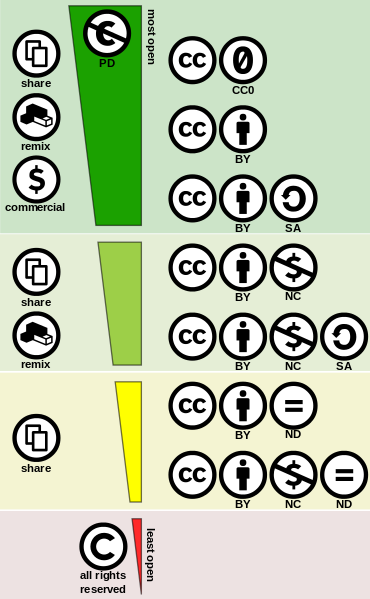
\includegraphics[width=.5\textwidth]{pictures/Creative_commons_license_spectrum}
 \caption[Creative commons license spectrum between public domain and all rights reserved.]{Creative commons license spectrum between public domain (top) and all rights reserved (bottom). Left side indicates the use-cases allowed, right side the license components. The dark green area indicates Free Cultural Works compatible licenses, the two green areas compatibility with the Remix culture. \href{https://commons.wikimedia.org/wiki/File:Creative_commons_license_spectrum.svg}{Image by Shaddim via Wikimedia Commons.}}
 \label{fig:ccspectrum}
\end{figure}

\ac{CC} emerged from those meetings and was established as a non-profit organization to address this mission. The original idea was to create a site where people could upload their works to share. That idea was abandoned, however, in favor of creating a set of licenses (in the case of (CC0 \ccZero), not a license but a dedication and in the case of (Public Domain \ccPublicDomain), a validation) that allow artists and creators to mark their works with the rights that they would like to permit for their works, such as allowing people to remix and reuse with attribution, or for non-commercial use only. These licenses had icons associated with the rights so that it was easy for people to see what rights were associated with a particular work. (See \autoref{fig:ccspectrum}.)

The licenses allowed artists and creators to make choices about the permissions they wish to grant. They could require attribution (BY \ccAttribution), forbid or allow modification (ND \ccNoDerivatives), prevent use for commercial purposes(NC \ccNonCommercial/\ccNonCommercialJP), or insist that any derivative work be shared under the same license --- share-alike (SA \ccShareAlike). These could be combined; for example, Wikipedia uses \ac{CC} (BY-SA \ccbysa) which requires attribution and for the derivatives to be shared with the same license. One of the key innovations of \ac{CC} was its communication of these licenses in multiple modes: icons, human readable ``deeds'' that described the license in an easy-to-understand way, ``lawyer readable deeds'' that are legal contracts rigorously developed through a global network of lawyers, and a machine readable system of metadata in various formats to allow software, services and other systems to understand the licenses.

When I joined \ac{CC} as a board member, we were in the process of trying to get the licenses ``ported'' to local jurisdictions around the world, to create a global network and to try to create an enduring organization to manage this.

\subsubsection{Public Domain and CC0 \ccZero}

My efforts to create a public domain mark illustrates the complexity of trying to build open spaces in a world that is connected but that differs deeply over the appropriate laws and norms.

During my time as CEO of \ac{CC} from April 2008 to March 2011, we launched (CC0 - \ccZero), known as ``the public domain license.'' By then the requirement for attribution was so commonly requested that it had become a default requirement in all of the core \ac{CC} licenses. But, we realized that there were cases where attribution was impossible and where marking the works as free of all obligations and as close to public domain as legally possible made sense. Our legal team, led by Diane Peters, worked to coordinate input from around the world to try to make something that worked as best as possible in every jurisdiction. Getting to a single document was a herculean effort.

We had previously had a Public Domain Dedication (renamed Public Domain Certification in 2005) that marked works as Public Domain. But that was confusing because the notion of ``Public Domain'' existed in the United States but not in all jurisdictions. When we launched (CC0 \ccZero), we also launched the Public Domain Guidelines that, together with (CC0 \ccZero), were a template of norms that communities could adopt in a way that was appropriate for them. It encouraged norms from the attribution (BY \ccAttribution) license such as provenance (link back), citation, etc. but in a way appropriate to their community and their medium and in a non-legally binding way --- policed through norms rather than law.

These guidelines were adopted by organizations such as Europeana, the massive online aggregation of European cultural works. The guidelines were in great part informed by those used in the scientific community for projects such as Polar Commons, one of the first users of (CC0 \ccZero).

In October 2010, we released a tool called Public Domain Mark (\ccPublicDomain) to mark works in the public domain. This was an important complement to the (CC0 \ccZero) dedication which was a tool for asserting, to the extent possible under the law, a waiver of rights for works that were not in the public domain. For example, the copyright on works by Herman Melville have long expired, so those works are in the Public Domain, and could be marked as such by the (Public Domain Mark \ccPublicDomain). But if you posted something tomorrow about Herman Melville, it would automatically be copyrighted. If you wanted instead to release the work as close as legally possible to being in the public domain, you would use the (CC0 \ccZero) dedication\footnote{Some legal jurisdictions do not allow you to completely waive all of your rights. (CC0 \ccZero) is a dedication that waives all right to the extent possible under the law. It is also a waiver of rights, and not a license.}. Europeana was requiring that metadata with licensing information be added to all thumbnails indexed on their site. They were planning on creating a Europe-only public domain mark for their site, but we were able to convince them to instead use our Public Domain Mark which that was usable worldwide. 

It gets yet more complicated. The U. S. Government considers works ``prepared by an officer or employee'' of the federal government to not have protection under domestic U.S. copyright laws and regulations. However, the U.S. Government asserts that its employees hold the copyright to these works in other countries. Most people imagine that U.S. Government works such as \ac{NASA} photos or government studies are in the public domain globally, but they in fact are not. This means that Wikipedia, which uses a (BY-SA \ccbysa) license, could not use, say, an image from \ac{NASA} because non-US people could access the pages.

\marginpar{We were emboldened by the fact that the White House had switched the copyright license for the White House website to a \ac{CC} (BY \ccby) license when President Obama was inaugurated.}I visited the White House, the Public Printers Office, and a number of agencies in the federal government to try to address this issue, arguing that this restriction made no sense and that preventing U.S. Government works from entering the worldwide commons was impinging on the impact of these works and went against the spirit of creating such works. We were emboldened by the fact that the White House had switched the copyright license for the White House website to a \ac{CC} (BY \ccby) license when President Obama was inaugurated.

With the help of Beth Novack, who was Deputy Chief Technology Officer of the US at the time, I tried to come up with a plan whereby each U.S. agency could use something similar to a (CC0 \ccZero) dedication to give up the international rights to their works so that Wikipedia and others could use \ac{NASA} images and other government works freely on the Internet. Eventually, I ended up at the \ac{GSA}, where I was told that federal agencies do not have the right to waive their copyright and that the international rights were ``assets of the federal government.'' Moreover, the \ac{GSA} controls the federal government's balance sheet and thus has to approve any such transactions.

This issue has still not been resolved and is still being actively pursued by \ac{CC}.

\subsubsection{Interoperability}

An issue came up in Europe around a right called a ``database right,'' which provided protection to databases or collections of works even if the individual works in the database weren't copyrighted or able to be copyrighted. The United States and many other jurisdictions didn't have such law or right, and addressing it in the (CC0 \ccZero) dedication or \ac{CC} licenses didn't make sense from a global perspective.

That led the Open Knowledge Foundation, a friendly partner in the United Kingdom that often helped us in the region, to create an Open Database License to deal with the database issue. But this license was not interoperable with and, in some cases, tried to replace \ac{CC} licenses. One key example was OpenStreetMap, an extremely important crowdsourced source of open maps used by many services such as Foursquare and Craigslist. OpenStreetMap originally used (BY-SA \ccbysa) license but the organization was convinced to convert to Open Knowledge's ODbL license. We had many conversations to try to keep them with \ac{CC}. While the ODbL dealt with database rights in a way that \ac{CC} didn't, we believed the benefits of ODbL didn't outweigh its cost, namely, that OpenStreetMap data would no longer be interoperable with other (BY-SA \ccbysa) works, including huge projects like Wikipedia.

Similar to technical protocols such as \ac{TCP/IP}, even if the legal ``code'' of the licenses are nearly identical, they are slightly different and make interoperability difficult, if not impossible. The key thing about share-alike or copy-left licenses is that they require derivative works to be licensed under the same license. So even if the licenses are nearly the same, because they are not the same license, the user can't switch the license. This keeps the works that are spiritually similar in intent, separated legally. One idea that many of us had was to create a section in the license that listed other, but similar licenses that the user could opt to relicense under. However, since licenses could be upgraded or changed, people didn't feel safe creating a list of compatible licenses because there was no assurance that they would continue to remain theoretically aligned.


In Open Source Software licenses and with those from \ac{CC}, we made efforts to find ways to make different licenses interoperable, but this also required a great deal of work and had limited success. The two most notable examples are the Mozilla Public License 2.0 defaulting \ac{GPL} compatibility and (SA \ccShareAlike) 4.0's compatibility mechanism that is used to make it \ac{GPL} compatible. Additionally, after Wikipedia migrated to (BY-SA \ccbysa), OGL-UK-2.0 and several other open government licenses were made explicitly \ac{CC} (BY \ccby) compatible.

One of the most significant relicense efforts was Wikipedia, which was created before \ac{CC} and established using the Free Document License that the Free Software Foundation created for the GNU free software project to allow free sharing of documentation for its software. It was designed for things more like books and so not well suited for the kind of remixing and editing that Wikipedia represented. For example, it required the distribution of the license with the software, rather than just a link to the software because it was designed before the Web. More importantly, it was not interoperable with the ever-growing body of \ac{CC} licensed works on the Internet because although it was a copy-left license\footnote{A copy-left license, like a share-alike license, allows works to be used freely as long as the derivative works are relicensed under the same agreement. This stipulation first popularized in the GPL software license forces free software to increase rather than just be reused and is the one of the core political features of free software.}, it did not allow relicensing under other licenses such as the \ac{CC} share-alike (SA \ccShareAlike) and therefore could not be remixed with \ac{CC} content that should otherwise have been compatible with Wikipedia.

After a great deal of discussion and negotiation with the Free Software Foundation and the Wikipedia community, \ac{CC} came up with a deal that allowed for a brief period a modification in the Free Document License. This modification allowed Wikipedia to convert its content to a \ac{CC} (BY-SA \ccbysa) license, and in 2009, supported by a community vote, we were able to convert Wikipedia from the Free Document License to a \ac{CC} (BY-SA \ccbysa) license, vastly increasing the body of work available under that license.

\subsubsection{Funding and Organization}

Idealistic intentions require realistic infrastructure. And that requires raising money and dealing with organizational issues. Yet even these activities can be approached in ways that represent the values and methods of antidisciplinarianism.

As a board member and before I became the CEO, I was actively involved in fundraising for \ac{CC}. Fundraising for causes that are hard to categorize and may appear to be ``infrastructure'' is quite challenging. Funders typically like to fund programs or ``verticals.'' In addition, there is a natural tendency for special projects to turn into bigger initiatives and spin out for programmatic and personality reasons.

When I became the CEO of \ac{CC}, we had three projects with separate funders and project leaders. One was ccLearn, which was dedicated to the development of Open Educational Resources (OER) and supporting the learning and education community. The William and Flora Hewlett Foundation funded it. We also had Science Commons, a project aimed at building a ``Creative Commons for Science'' that would focus on issues such as patents and materials transfer agreements. We also had a separate office working on \ac{CC}'s international effort and headquartered in Berlin. Lastly, we had created a group called iCommons. ``The aim of iCommons reaches far beyond the infrastructure that \ac{CC} is building. The aim of the iSummit is to bring together a wide range of people in addition the \ac{CC} crowd --- including Wikipedians, Free Software sorts, the Free Culture kids, Access to Knowledge heroes, Open Access advocates, and others --- to 'to inspire and learn from one another and establish closer working relationships around a set of incubator projects'' \cite{iCommons18:online}.

While each of these projects had a strong mission and purpose, I felt that they were fragmenting the organization and impairing its management and community dynamics. One of the largest efforts --- an intervention that I led with the board and staff --- was to consolidate all of these projects into a single \ac{CC} organization. iCommons, which was already a separate legal organization was made more clearly independent. This clarification and consolidation made \ac{CC} a more integrated and international organization.

One of the keys to success of the \ac{CC} organization and its community was the relationship between the central organization and its regional affiliates. The central organization was a dedicated group of exceptional staff with deep technical, legal and domain expertise in fields such as science, arts and publishing. We had relationships in over 70 jurisdictions, which allowed those partners to use our brand and trademark as long as they adhered to the guidelines in the agreements we struck with them. The use of trademark and brand to manage a network of affiliates had been used in the past, but our use of this structure was quite advanced and effective. Unlike businesses, we did not have a financial relationship with the affiliates and the ``currency'' was the brand. The strength of the brand was sufficient to enforce a high level of adherence to obligations.

 \ac{CC} was not the only organization to strictly protect its trademark while allowing content to be free and open; the Mozilla Foundation takes a similar approach. It provides a useful tool for managing commons-based organizations that rely upon an extended community.

\marginpar{One of the hardest problems was how to keep volunteers --- often the majority of the labor --- sufficiently motivated and organized.}As part of our effort to build a global community while respecting the differences in culture and legal environments, we also ran highly effective international meetings where community members could communicate, collaborate and build trust. We had an extremely diverse group of people in our community ranging from federal judges to artists to communist activists. They nonetheless were able to come together to support a common cause. Strong bonds were built. These connections across traditional boundaries have become an extremely important part of the \ac{CC} community. The events were also critical in providing a way for the volunteers to feel actively involved, and for us to have both difficult and delightful conversations --- I do not think that the organization could have survived at its scale without these physical meetings.

The integration effort, the trademark management, the organization of the international conferences, and the organization in general shared some common themes that we learned and continued to develop, sharing best practices with other organizations with similar structures. One of the hardest problems was how to keep volunteers --- often the majority of the labor --- sufficiently motivated and organized. With a core paid staff, there was always a ``difference in class'' issue with the unpaid volunteers. Also, deciding who was allowed to speak on behalf of \ac{CC} and on what topics, was a key issue that needed to be well managed.

The board of directors was originally all US-based and mostly academic. Over the years, we included a broader representation of geographies and fields.

Managing the brand was key. We needed the kid who wore the \ac{CC} t-shirt and marched in the streets against bad politicians to feel like part of the ``tribe'' but to also make it clear when we were negotiating with the UN which individuals in our system were qualified and authorized to speak on our behalf. The public as well as internal management of inclusion and tight control of key roles appears to similar in every successful open project that I've ever participated in and something that can be applied even to university campuses or companies.

I personally feel a need to point out that all of this online activity occurs in a real world that can impose very real costs. I will always remember Bassel Safadi, a tremendously important member of our community and a key person in developing the work of \ac{CC} in the Arab region, as well as building bridges with other regions. Thanks to Bassel and an exceptional group of colleagues in the region, we launched a set of Egyptian \ac{CC} licenses in 2013. This effort took years of work and many difficult meetings requiring us to learn the relationship between the different countries, the culture, the role of law in the region and bridging many fundamental differences with systems. Bassel was later imprisoned and murdered by the Syrian Government.

We don't know if his work for \ac{CC} played a role in his death. But Bassel's absence reminds us that the funding and organizational work are in service to communities of people who have dedicated themselves to making the world better, often against long odds. These communities are the most significant asset that \ac{CC}, and the Media Lab, have developed.

\subsubsection {Continuing the Work}

While some services such as Flickr made \ac{CC} licenses available to users uploading material as a core part of the services they offered, it took years of work to persuade YouTube, Google and many of the large Internet platforms to embrace our licenses.

I remember giving a talk at a publishers conference many years ago where I shared the vision of \ac{CC}, explaining that its licenses helped authors who wished to share their works without making people ask them for permission. When I finished, the first publisher to rise to comment said, ``I think your comments are disgusting.'' She pretty much summed up the feeling in the room. 

We've come a long way. In March 2018, I gave the keynote address at the MIT Library conference on Grand Challenges where I was asked to talk about open scholarship. I noted that even the publisher with the most stringent copyrights, Elsevier, now uses \ac{CC} licenses to mark their Open Access works and that \ac{CC} has become a common default for publishers, authors and others to assign whatever rights they wish to their works. Many foundations now require their grantees to publish their works under \ac{cc} licenses, and the licenses have become a key element of the Open Access movement to free academic works for sharing, and for scientists to use the Internet to its full potential.

\subsection{The Open Source Initiative}
\label{sec:OSI}


\cite{Historyo84:online}:
\begin{quotation}
Development based on the sharing and collaborative improvement of software source code has a history essentially as long as software development itself. In the late 1990s, interest and participation in this phenomenon increased markedly with mainstream recognition of Linux in publications like Forbes and the release of the Netscape browser’s source code.

The \ac{OSI} was formed in 1998 as an educational, advocacy, and stewardship organization at the important moment in the history of collaborative development.
\end{quotation}

Founded in 1998, \ac{OSI} was a campaign to promote open source software. Having created the ``\href{https://opensource.org/osd}{Open Source Definition}'' that became a standard definition for ``open source.'' \ac{OSI} developed a board of directors and became the organization that reviewed and ``approved'' open source licenses tested against the Open Source Definition and granted permission to use the \ac{OSI} mark.

\begin{figure}[h]
 \centering
 
\includegraphics[width=.5\textwidth]{pictures/Opensource}
 \caption{The \ac{OSI} logo}
 \label{fig:OSI}
\end{figure}


The organization also aimed at pushing back against what many believed was an effort by commercial software companies to fight the move toward free and open source software. These fears gained credibility when, in October 1998, confidential documents known as the ``Halloween Documents'' \cite{Hallowee48:online} were leaked to Eric Raymond. They revealed Microsoft's strategy against Linux and Open Source software, confirming the community's fears that Microsoft and others were engaging in an all-out war against Open Source.

I joined the \ac{OSI} board in May 2005 and served for two years and two months. During this period we worked on a number of issues.

One issue was license proliferation. Just as with \ac{CC} licenses, the interoperability of \ac{OSI}'s licenses was crucial, but the number of similar yet incompatible licenses was growing. There were already a number of open source licenses, but during my tenure, we saw a number of ``vanity'' licenses being created: licenses created by companies or communities solely for their own projects and with little consideration for the damage to interoperability. As with \ac{CC} licenses, small changes made software licensed under these modified derivative licenses incompatible with other software licenses, preventing developers from combining code from different projects. Having too many licenses to choose from also made it difficult for developers to choose one. 

We decided to intervene and embarked on a mission to try to talk people out of vanity licenses. We were successful in getting a number of licensees deprecated, including Intel's own Intel Open Source License \cite{LicenseP82:online} ; it was nearly the same as the popular BSD license, but with a clause regarding export laws.

\marginpar{A key learning for me was that with open protocols there is a period where many ideas proliferate and innovation occurs. This is important. However, it is important to work on converging the standards as the network and projects deploy.}Nations are one of the more stubborn ``disciplinary boundaries'' we face as we try to build global communities and communities of practice in a world that is always local. We saw this again with the Mozilla license. (I later served on the Mozilla Foundation board.) It stipulated that disputes must be handled in Santa Clara County, California, but most companies basing their license on the Mozilla license substituted their own jurisdiction, which created a substantial number of incompatible but very similar licenses. This was eventually resolved in \href{https://opensource.org/licenses/MPL-2.0}{version 2} which set the jurisdiction to ``where the defendant maintains its principal place of business.''

A key learning for me was that with open protocols there is a period where many ideas proliferate and innovation occurs. This is important. However, it is important to work on converging the standards as the network and projects deploy. For example, in the cryptocurrency space, we see a proliferation of blockchain technologies, that will hopefully begin to converge soon.

During my \ac{OSI} tenure, the key to the success of \ac{OSI} was the strong leadership of Michael Tiemann and Danese Cooper.I learned a great deal from their management of the organization and the stakeholders.

\subsection{Blockchain and Questioning Sovereignty}

Blockchain has become the IT ``fad du jour'' and is being touted as the solution for almost everything. It is clearly hyped right now, but the ideas behind it have been around for a long time and I believe that the impact will be larger, different and later than most believe. Similar to the Internet, its decentralizing and unbundling architecture will drive a similar, if not equivalent, change in the finance and legal fields as well as in other sectors.

In 1995 I predicted that ``for world economies, like a brand new foreign exchange system using digital cash, or a new stock market based on digital transactions --- those are really great visions that will happen, but they will happen based on a need'' \cite{EccosysI53:online}. The next year, I wrote a book about digital cash \cite{digitalcash} with Takao Nakamura, who left the Bank of Japan to join me at the startup I co-founded, Digital Garage. The book surveyed the digital currency projects at the time and charted a vision for the future of digital currencies and electronic payments.

Then my team at Eccosys and I set up a DigiCash server (199.100.7.5) and established an Ecash Merchant account that allowed us to send and receive Mark Twain Ecash, a gold-backed digital currency issued by the Mark Twain Bank in the US. We sold music and images on the Tomigaya website, but DigiCash did not take off and and went bankrupt in 1998. The excitement around digital cash dwindled, although digital payments and settlements continued.

In 1999, Digital Garage, and Lawson's, the convenience store chain, began working together on the idea of turning convenience stores into payment gateways using the Lawson Loppi terminals in the company's stores. I worked with the Digital Garage team to sell the president of Lawson, Naoki Fujiwara, and his team on the vision and help them think about potential applications. Digital Garage, Lawson, Mitsubishi Corporation and TIS Inc. then created a joint venture called eContext, which would become one of the largest settlements company in Japan. The eContext Asia group is a global network and went public at Hong Kong Stock Exchange in 2013. It is now a 100\% subsidiary of Digital Garage.

\subsubsection{Managing disagreement: Cypherpunks}

My work on digital payments piqued my curiosity about cryptography and the Internet, and I got actively involved in the Cypherpunks community, an informal group of hackers who worked on cryptography, networks, and systems. I was fairly active on the group's mailing list, which was the place where most conversations occurred, and I worked to bridge communications between Japanese researchers, governments, and this community. In 1997, I attended a conference in Amsterdam called ``Hacking in Progress,'' which took place in the middle of a forest. The Cypherpunks had set up a tent, where I was able to connect with many community members from Europe as well as the United States.

Many of the key developers and thinkers from this early period are the leaders of the current cryptocurrency field. Many of the ideas that sound new today were hatched during this early Cypherpunk period.

Establishing a conversation between government regulators and the decidedly anarchical Cypherpunk community was never easy. Here's is an example of my attempt to get feedback on some ideas for a Japanese National Police Agency study group. This is from the notorious Cypherpunks mailing list. Tim May is one of the co-founders of the list.

\begin{verbatim}To: Joichi Ito <jito@eccosys.com>, cypherpunks@cyberpass.net
Subject: Joichi Ito as a Junior Policeman
From: Tim May <tcmay@got.net>
Date: Fri, 1 Aug 1997 23:46:56 -0700
In-Reply-To: <199708020550.OAA04024@eccosys.com>
Sender: owner-cypherpunks@Algebra.COM

At 10:31 PM -0700 8/1/97, Joichi Ito wrote:

>I can't tell you about any of the other stuff that is currently being
>presented
>in the study group, but once the report becomes public, I will try to get
>an English version up on the Net. It should end up being the Japanese
>National Poice Agency's official position on Key Escrow, Certification
>Authorities, and several other issues.

And why are you helping to write a report that will be the "official
position" of the Japanese cops?


>I will be participating in another study group soon to discuss many of
>these issues with the Self Defense Force from the point of view of
>Japanese national security as well as another NPA study group on
>what to do about "crackers"... Anyway, if anyone who can give me some
>insight into these areas will be at HIP, I'd love to chat. ;-)

And why are working for the "Self Defense Force" (the Japanese DOD, for
those not familiar with the terminology).

The JDF is notoriously militaristic. You should reconsider this.

And Cypherpunks should be very careful about "advising" an obviously
co-opted member of the Japanese military and police establishment.

Use crypto to undermine such entities, not support them. Crypto will
unleash anarchy on the world.

>Thanks again.
>
>- Joi
>
>P.S. I am not a "policeman" but an outside board member of these
>study groups. The ministries are under quite a bit of scrutiny these
>days and the study groups tend to be quite frank and balanced.
>The reports don't always dictate the law, but since most politicians
>do not have real staffers, therefore most of the expert study
>is done in the ministries.

You sound like a "junior policeman" to me.

Another person to add to the killfiles.

--TCM

--
From: Tim May <tcmay@got.net>
Subject: Re: Tim Throws a "Leaner" / Re: Tim Speaks the Truth
Date: August 3, 1997 at 22:02:24 PDT
To: cypherpunks@algebra.com
Cc: jito@eccosys.com

At 8:46 PM -0700 8/3/97, Anonymous wrote:
>Joichi Ito wrote:
>>As for Tim's message... I keep worrying (when I am in Japan)
>>that I'm too radical, so it's nice to hear from someone who
>>is really hardcore to put a wimp like me in my place. ;-P
>
Actually, when Tim puts someone in what he considers to be their
place,
it usually involves the purchase of a tombstone.

Actually, the trick is to avoid having the body discovered.
What goes into the 10 h.p TroyBilt Chipper/Shredder comes out
not needing any kind of tombstone at all.

Not that I have ever advocated killing mere folks like Joichi
with whom I disagree strongly. (A new quote: "Killfiles don't
need tombstones.")
\end{verbatim}

While the players have gotten older, the style and the tone of many of the conversations on mailing lists about Bitcoin are very similar. This is one of the difficulties that we have in the community today. The style of these conversations on mailing lists or \ac{IRC} are a combination of very sophisticated technical discussions and sometimes childish or politically insensitive interchanges. Bringing government, academia, and the Cypherpunk-turned-cryptocurrency community together remains a non-trivial exercise that I am still engaged in. It's harder than organizing the Internet community; although the Internet old-timers were a bit hippie-like, they were mostly academic and often government funded. So while, they weren't different from their buttoned down government counterparts, there wasn't nearly the kind of gap that exists in the Cypherpunk-government-industry trifecta.

I visited and met with many of the Cypherpunks in the United States and organized visits for them to speak in Japan. I also helped Shuichiro Hanabusa from NHK produce a special called ``Crypto Wars,'' about the Cypherpunks movement. I had conversations with the Bank of Japan and \ac{NTT} Data, which were conducting a digital cash trial. The Bank of Japan was unhappy about some of my public comments about digital currencies, and Mitsuru Iwamura at the \ac{BOJ}'s Institute for Monetary and Economic Studies even canceled a talk I was invited to give at there. Later, Iwamura-san became my mentor. I also got to know Naoyuki Iwashita, who later became head of the \ac{BOJ} FinTech Center.

% \subsubsection{Electronic Signature Service\dw{Candidate for deletion}}

% Mart Saarepera, a cryptography researcher, began working for me at my incubator, Neoteny, in 2001, trying to develop a mechanism platform for authentication and digital signing, or Electronic Signature Service (ESS), with the following properties:
% \begin{itemize}
% \item Low cost compared to PKI (X.509 and similar) and user-owned hardware devices such as smartcards
% \item Easy usability based on software and web interface
% \item Robustness --- highly reliable platform built from components with low reliability
% \item High availability --- scalable to at least 150M users
% \item Patent protection
% \end{itemize}

% I approached \ac{NTT} Data about investing in the project, and we also presented it to officials in Yokohama and those responsible for Japanese Digital Signature Act.

% My business development staff at Neoteny made considerable efforts to justify the market hypotheses for ESS but were unable to develop a plan that regulators or businesses would agree to. In 2002, we presented the project to Professor Jiro Kokuryo at Keio University, and in the spring of the following year, Professor Kokuryo used the project as a case in his International 
% \ac{MBA} course and created a team project to develop a viable business plan.

% Two patent applications were filed, ``System and method for renewing and extending digitally signed certificates'' \cite{saarepera2004system} and an application named ``Fast Signature.’’ A year later we discovered the application by Eric Hughes (US2002/0184504 A1) describing exactly the same invention few months before us.

% The key technical features of Neoteny ESS were published a series of academic papers \cite{ansper2001improving, buldas2003electronic}.


% \subsubsection{Time Stamping Service \dw{Candidate for deletion}}

% In 2003, \ac{NTT} Data suggested a joint project with Neoteny to develop a time-stamping system that the company could use to replace its existing time-stamping service. At the time, \ac{NTT} Data was using a hash-chain-based time-stamping platform licensed from Surety Inc. 

% \textbf{Motivation and Goals}

% The goal of the project was to develop a next-level, version 2.0 time-stamping system platform with the following properties:
% \begin{itemize}
% \item Robustness --- high reliability platform built from low reliability components
% \item High availability --- scalability to millions of clients
% \item IP protectability as Surety had six patents and numerous other patents existed in the field
% \end{itemize}

% \textbf{Project Summary}

% We engaged in a two-month project beginning in June 2003, after having completed a patent infringement analysis in the prior year. As a result, a new hash-chain-based time-stamping system satisfying the \ac{NTT} Data criteria was proposed. One patent application was created \cite{saarepera2010system} and all the key technical results were published in two academic papers \cite{buldas2004provably, buldas2005universally}.

% But \ac{NTT} Data eventually decided not to invest in the project, so the research was continued as a PhD thesis \cite{villemson2002size} supervised by Ahto Buldas. 

% In 2006, the TSS was commercialized under the name Guardtime AS (www.guardtime.com) and is now a leading industrial block-chain provider.

% While this project was ultimately successful, we ended up spending a lot of time working with and talking to large companies. This is exactly the kind of academic to business collaboration that has become so much easier, but this work in 2003 with the digital signatures and time stamping was my initial attempt to do deep R\&D with academics. My key lessons were that we should have been more tightly integrated into the US venture community and the cypherpunk community. 

% \subsubsection{Electronic Cash and Payment Systems \dw{Candidate for deletion}}

% In late 2001, Ahto Buldas attended an ISO standards meeting on time-stamping in Tokyo. He gave a presentation at Neoteny about the state of the art of digitized cash. Professor Mitsuru Iwamura of Waseda University, together with the chief cryptographer at Hitachi, Rojoichi Sasaki were invited, but only Dr. Sasaki attended. 

% Buldas’s presented work on Estonia, where 97 percent of bank transactions had been digitalized but no cash was digitalized. He described the Estonian digital banking system where Internet banks were widely and efficiently used as payment systems. He explained that the efficiency of the system was due to an inter-bank clearing system that charged only a small transaction fee. 

% The scalability of such a payment system as a whole, Buldas told us, depended on the scalability of two independent systems: the intra-bank transaction system and the interbank clearing system. Intra-bank transaction systems are instantaneous, but the speed of interbank payments depends on the clearing system and the main question was whether the clearing system could scale

% Interbank clearing is technically easily to achieve, but it depends on trust relationships between banks. Since trust between two banks is unpredictable, it was impossible to develop an efficient interbank clearing system. 

% So Buldas concluded that the only way to make electronic payments scalable was to digitize cash, or create electronic money. Our team was authorized to work on electronic payment systems and on digital money.

% \subsubsection{Neoteny Digital Money}

% Dr. Iwamura and Dr. Iwashita, our advisers, urged us not try to tackle the problem of digitizing electronic cash, however.

% Saarepera and the team spent a great deal of time trying to find ways to digitalize alternatives to digital money like bearer bonds. Jay Dvivedi, chief investment officer of Shinsei Bank and a Neoteny adviser, pointed out that this effort might be meaningless in Japan. Then Neoteny commissioned an analysis by Deloite-Tohmatsu, which strongly discouraged the team from working on digitalization of cash alternatives such securities, collateral and valuables belonging to clients and suggested we work towards digitalization of electronic documents in general. 

\subsubsection{Early Exploration on Cryptocurrencies}

Some time before September 2001, Sen Nagata, Neoteny's head of R\&D, approached Saarepera about electronic cash and a payment system similar to what we know as Bitcoin today. Nagata asked a series of feasibility questions about a system that would combine a bank and a payment channel, including whether it was possible to have:
\begin{itemize}
\item A model of a payment transaction between pseudonymous accounts 
\item A unique ledger of transactions with a formal correctness condition (predicate) 
\item A stack machine for transaction processing
\item Distributed control of accounts (multi-signature authentication)
\item Cash transfer authorization
\item Cash emission as a special transaction
\item Proof of work, similar to HashCash that guarantees uniqueness of the ledger
\end{itemize}

All the listed items seemed feasible by our team, except the proof of work. We knew about a proof of work from HashCash \cite{back1997hashcash} as a potentially practical anti-spam measure. Saarepera and Nagata had many discussions and concluded that proof of work would guarantee the uniqueness of a ledger only if there was a single ledger and there is not sufficient computational power anywhere to create another one. If we had more than one ledger, proof of work could not be used as a uniqueness criterion.

\marginpar{This early exploration by Sen Nagata is basically Bitcoin. We could have invented it and deployed it years before the Satoshi Nakamoto white paper.}While the work on digital money helped lead to the creation of eContext inside of Digital Garage and sparked my collaboration with Lawson, we should have pushed harder to try to develop true digital cash. This early exploration by Sen Nagata is basically Bitcoin. We could have invented it and deployed it years before the Satoshi Nakamoto white paper.

We may have been too early, but my lesson learned is to not give up on radical ideas just because people tell you that you can't do it. :-)

\subsubsection{Havenco}
\label{sec:havenco}

As the same time that I was straddling the line between hackers and government, I became interested in the cross-border repercussions of the Internet and the role that cryptography and the Internet would play in trade and contracts. I worked with the United Nations Commission on International Trade Law to come up with rules for arbitration in cyberspace, and in May 1999, I presented a proposal for cyber-arbitration at a meeting of the Inter-Pacific Bar Association. The same year, I also worked with the Japanese Ministry of Trade and Industry on the Japanese response to the first discussion of electronic communications at the World Trade Organization. 

I created demos, sat in many long meetings but we never deployed. Lesson : working with government is slow work.

Working on Havenco was the opposite of working with big government.

\begin{figure}[h]
 \centering
 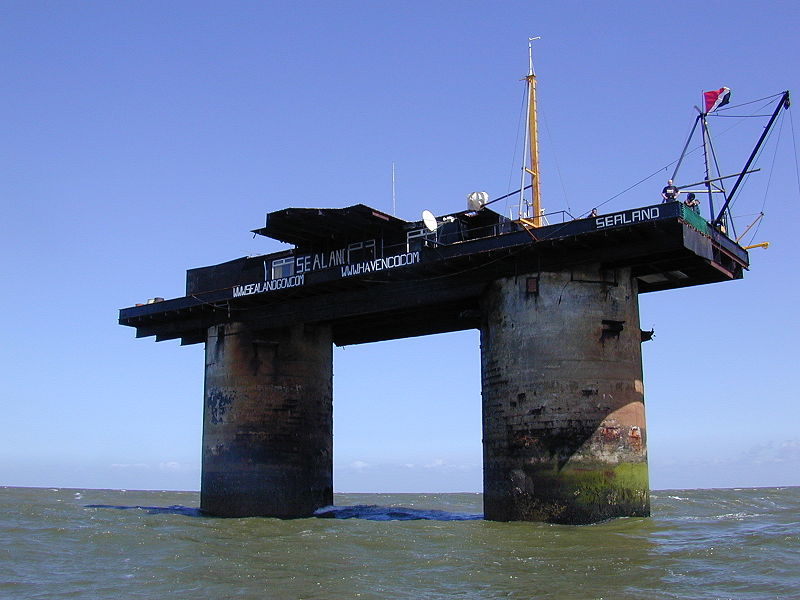
\includegraphics[width=0.5\textwidth]{pictures/sealand}
 \caption{The Principality of Sealand where we ran the Havenco business. Photo by Ryan Lackey.}
 \label{fig:sealand}
\end{figure}

\marginpar{In 2000 it was technically difficult to establish communications with an aircraft platform in the sea. Doing so required a team of engineers and armed guards to live on this old anti-aircraft platform.}In 2000, I took up a quirky project to develop a data center business called Havenco on the Principality of Sealand (see \autoref{fig:sealand}, a tiny nation established on an offshore platform located in the North Sea off the coast of Suffolk, England. We could protect these servers from government spying or seizure --- at least that was the idea. Wired ran the Sealand experiment as a cover story that year \cite{garfinkel2000welcome}.

In the year 2000, Wired Magazine devoted its cover to a story about Havenco \cite{garfinkel2000welcome}. The idea of the company was to take John Perry Barlow's 1996 Declaration of the Independence of Cyberspace \cite{barlow1996declaration} literally and create a co-location/data center in a sovereign jurisdiction that we controlled. 

I met a group of Cypherpunks --- Ryan Lacky, Sean Hastings, Jo Hastings, Avi Freedman and Sameer Parekh --- that were in discussions with the Bates family, who had declared their World War II anti-aircraft platform off of the shore of England a sovereign state: Sealand. They cited salvage law since it was abandoned. At one point, they had fired on the British Navy and were taken to court and their position was upheld.

I became an advisor and an investor and embarked on one of the most interesting but craziest ventures I have ever been involved in.

In 2000 it was technically difficult to establish communications with an aircraft platform in the sea. Doing so required a team of engineers and armed guards to live on this old anti-aircraft platform. (Luckily, I wasn't part of the operations team.) One of the main costs was fuel to power the generators.

The venture was a really interesting idea, but it was early, the team was not experienced enough, and it was a really hard problem. Unfortunately, the project ended before we were able to test some of the more interesting questions in court or on the battlefield.

While it was ultimately unsuccessful, the project was possibly the closest any group has ever gotten to creating a jurisdictionally independent data haven akin to Barlow's vision.

The business plan of Havenco is in \autoref{ch:havenco}.

Through the process of planning and operating the company, we explored in a very real way the challenges and opportunities global communications infrastructures like the Internet face. While inter-jurisdictional challenges were being actively addressed, strange exceptions like Havenco provide an opportunity to imagine other structures. These might come into play again when we start sending servers into space or in the deep sea.

\subsubsection{Bitcoin}
\label{sec:DCI}

In 2008, a person or group of people calling himself or themselves Satoshi Nakamoto (we still don't know who this is) published a paper, ``Bitcoin: A Peer-to-Peer Electronic Cash System'' \cite{nakamoto2008Bitcoin} that kicked off a cryptocurrency mania. The craze started slowly, and I watched it with only mild interest.

But in 2014, Jeremy Rubin, an undergraduate student involved in the MIT Bitcoin Club, nagged me to be the principal investigator on a project aimed at distributing Bitcoin to students to see how they would use it. I was the co-\ac{PI} with Christian Catalini from the Sloan School of Management at MIT. Because of this project, I became more involved in Bitcoin research and supported Jeremy and others who were working in the space. The work was published on their website.

The Bitcoin Foundation became imperiled with an imminent bankruptcy in early 2015. Jeremy and I hatched a rescue plan with support from Adam Back, Pindar Wong, and others in the Bitcoin community. We raised funds and hired key core developers who were supported by the foundation, including the former and present lead maintainer of the Bitcoin project. We created the \ac{DCI} at the MIT Media Lab to house these developers and serve as a nexus for cryptocurrency research.

We have assembled an extremely diverse, relevant and high quality team of experts at the \ac{DCI}, giving preference to those with no commercial interests in any fintech startups or currencies. Directed by Neha Narula under my guidance, the \ac{DCI} has recruited Simon Johnson, the former chief economist of the \ac{IMF}; Robleh Ali, the former head of digital currencies of the Bank of England; Tadge Dryja, the co-founder of the Lightning Network, and Gary Gensler, the former chairman of the Commodity Futures Trading Commission. Our core team is working closely with central banks, regulators and the \ac{IMF}, World Bank, the Inter-American Development Bank (IADB) and others to think and develop long term strategies and protocols that are less concerned about making money and more concerned about creating a working, resilient and decentralized financial system and system of distributed trust. One of the risk of the current focus on for-profit fintech companies is that their focus on financial returns for their founders and investors are driving them to think shorter term and less about a common interoperable infrastructure.

While we still have a long way to go, our work to establish the nonprofit layers of the Blockchain stack is key in trying to make sure that we can create a Blockchain future with fair, functional and interoperable protocol layers, and generative and productive commercial layers in between, following the Internet's model.

The \ac{DCI} has also helped organize the Scaling Bitcoin conference series, which has served as a neutral meeting ground for Bitcoin developers and scientists to discuss the latest research. The first two instances of the event in late 2015 helped diffuse tensions building around the debate over block size, and at the second event, Pieter Wuille, a prominent Bitcoin developer, announced SegWit, or ``segregated witness,'' which offered a way to limit block size; it has become the focus of the technical debate ever since.

Dr. Narula has a background in distributed systems. She and the \ac{DCI} currently are working on the following:

\begin{itemize}
\item Supporting core Bitcoin development
\item Attacking pressing problems to deploy cryptocurrencies in the real world --- for example, how do we provide privacy along with support for insight and financial regulation? How can we create new ways of proving that institutions are complying with financial regulation?
\item Figuring out Layer 2 (not to be confused with layer 2 of the Open Systems Interconnection (OSI) stack) --- blockchains fundamentally don't scale and Ethereum's model of executing every step of every smart contract on chain isn't going to work. We are exploring ways of making payments and smart contracts off-chain, while anchoring trust back onto the blockchain.
\item Redesigning the way that Bitcoin validates transactions to drastically reduce the cost of running a full node 
\item How to take lessons from cryptocurrency and apply them to the problem of designing a digital fiat currency
\end{itemize}

\subsection{The Startup Ecosystem}

My experience as an entrepreneur and a participant in the protocol and non-profit layers of the Internet has been key to my understanding and success at both. 

The Internet startup ecosystem is one of the best examples of the decentralization caused by the diminishing cost of innovation. In \textit{Regional Advantage}, AnnaLee Saxenian describes the shift of innovation from the Boston area to Silicon Valley as innovation in computers shifted from big companies and research labs with lots of money and equipment to smaller startups in Silicon Valley \cite{saxenian1996regional}. This push of innovation to the edges was an extremely important architecture shift that increased generativity in the commercial layers of the Internet. 

In 1999, I set up an incubator called Neoteny, which means the retention of childlike attributes into adulthood. It can refer to all the great things you often lose in adulthood, such as curiosity, playfulness, imagination, joy, humor and wonder. I first learned about the word from Timothy Leary \cite{TheMeani97:online}. I established Neoteny to help startups in Japan develop and as a way for me to develop and support the ecosystem of startups there by applying what I had learned as a startup entrepreneur to . After raising tens of millions of dollars from investors, I rented space and hired forty very smart people to support the startups. I learned the hard way that the cost and management overhead of running a full-service incubator was not commensurate to the value it would add to startups, at least the way I had designed it. The market crashed just after we got started, and publicly traded incubators that were trading at many multiples of the value of their portfolios started trading at a discount to their portfolios. We struggled to morph the model into a consulting company, but I realized that it wasn’t working and eventually let almost everyone go, and returned the remaining money to investors. It was an expensive lesson, but we did some important and original work on cryptography in the R\&D unit that I will describe in the next section. The people who worked at the company, whom I feared I had harmed greatly, developed a strong bond that continues today in the form of collaborations and reunions. Many of the alumni have been very successful in startup ecosystems around the world. 

During this period, I met the now well-known Silicon Valley investor Reid Hoffman. While at Neoteny, I helped him with his strategy to bring PayPal (where he was then an executive vice president) to Japan. I used my relationships at the Bank of Japan to secure a letter explaining how not to be regulated in Japan --- they just needed not to provide any services in Japan. PayPal successfully launched in Japan and Reid and I became friends. I continued investing as an angel investor, learning about the Silicon Valley ecosystem and comparing its robustness with the Japanese startup ecosystem. I realized that the style and network of investors in Silicon Valley, as well as the risk averseness of Japanese entrepreneurs, made a significant difference in the strength of the ecosystem, and I redirected my focus to Silicon Valley. 

After the dot-com bubble burst, sending the prices of technology companies listed on NASDAQ down to pre-Internet levels, Silicon Valley was cleared of irrational exuberance and left with entrepreneurs and investors that truly loved the technology and the work. I invested in a number of companies with Reid, including Flickr and Last.fm, and began developing a network of entrepreneurs and venture capitalists in the region. 

I also began exploring startup ecosystems around the world, including connecting with the community in Singapore, which was more entrepreneurial than Japan. The Singapore government was excited about supporting the ecosystem of startups there. In 2009, I set up venture fund (I currently call it Neoteny 2) with a special provision from the Singapore government that would provide a convertible loan worth 6 times the amount that I would invest in a startup if the startup were domiciled in Singapore. I could buy out the loan at cost, which effectively would provide me with 6 times the upside exposure for the same investment amount — a great deal. Singapore would help me with visas and many other things. I designed the fund so that it was also permitted to invest in non-Singaporean companies. The fund was successful, but ironically through companies that did not use the government incentive.

\marginpar{While some people focused on a particular layer and devoted their life to the development and stewardship of that layers, I expanded the layers that I participated in and used the contact that I had with each layer to try to coordinate and develop a kind of sensibility across the layers.}

From this experience I learned that startups are great for speed, execution and a certain kind of innovation and creativity, but the short-term nature of funding eventually drives companies towards profits and away from many of the societal goals and bigger ideas that may have provided their initial impetus. (This is obviously one reason I was excited to join the Media Lab.) I also found that I personally do not enjoy spending time with most venture capitalists. While they are more thoughtful and less zero-sum than most financial types, the conversations still revolve around money and how to make it. 

I also learned that success in a competitive venture ecosystem is not just being competitive or a hard negotiator, but adding value to the companies and the ecosystem. Great entrepreneurs and companies have their pick of investors; for the best companies, it's a seller's market. Venture capitalists that are successful are generally, although not always, very helpful, smart, friendly, and collaborative. The key to success is to be invited into a round by an entrepreneur or another investor because of what you can contribute to the company --- connections, mentoring, ideas, elbow grease. In successful and vibrant startup ecosystems, a network of investors that will take big bets on big ideas and not push companies to profitability too early is important to establishing ecosystems like Silicon Valley. 

The difficulty is that such an ecosystem requires good entrepreneurs, professional managers and technologists, and a critical mass. It is very difficult to start an ecosystem from scratch, as I learned in Singapore. Boston has an interesting ecosystem, very different from Silicon Valley’s. Boston’s strengths are biotech and the connection to the city's vibrant academic community. During a recent confab in Silicon Valley, nearly all of the leaders said that they ``wouldn't notice'' if Stanford disappeared. No one in the Boston area would say that about Harvard or MIT. The argument was that Silicon Valley attracted talent from around the world, from Stanford and MIT and Harvard, so it didn't matter that Stanford was close by. While the diminishing cost of innovation did push innovation to ``the edges'' and away from big, institutional R\&D centers, it ended up creating a localized ecosystem because of the value of face-to-face interaction and the ability to recruit as companies scaled. Silicon Valley is the clear leader and so is sort of a ``center'' now and not an ``edge.'' 

I believe that biotech has a different formula for developing and commercializing technology and that models such as PureTech Health, which I describe later in this chapter, are possibly more suitable.

% \section{Building a New Public Sphere}
% \label{publicspherepractice}

\subsection{Building Layers of Interoperability}
\label{sec:PSI}

As I participated in building various layers of the Internet, my experience and access to the community of the lower layers, gave me access to, and a starting point for, helping to build the next layers. While some people focused on a particular layer and devoted their life to the development and stewardship of that layers, I expanded the layers that I participated in and used the contact that I had with each layer to try to coordinate and develop a kind of sensibility across the layers.

\begin{figure}[h]
 \centering
 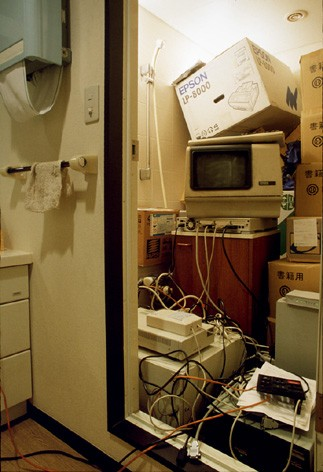
\includegraphics[width=.5\textwidth]{pictures/Joibathroompop1994.jpg}
 \caption{The PSINet point of presence in my bathroom circa 1994}
 \label{bathroompop}
\end{figure}

One of the benefits of having a 128K leased line to the Internet and the first commercial Internet service provider in Japan in my bathroom in 1993 was that it attracted hackers.

At \ac{ASIJ}, I used to co-run the Computer Club, and Cyrus Shaoul, a former \ac{ASIJ} Computer Club member (much younger than me) and a recent graduate of MIT reached out after he read an article by Howard Rheingold about my Multi User Dungeons (MUD) obsession \cite{kelly1993dragon}. He brought with him several friends including Daishi Harada, another MIT alum, and Sen Nagata and and Jonathan Haggan, both \ac{ASIJ} alumni. They all started hanging out (and sleeping) at my apartment, turning it into a hackers den where we worked on the new Internet software toys as they came out. We did a lot of work with early slowscan TV and CU-SeeMe, WAIS, Gopher, an anonymous remailer, a listserv and eventually the NCSA HTTPd server, which we used to set up our website in 1993.

When we set up our first real website, called ``Tomigaya,'' at \href{https://web.archive.org/web/19961227001638/http://eccosys.com:80/}{eccosys.com} in 1994, it was one of just a handful of websites in Japan. It became the home of many experiments, including an ecash site that sold music and images in exchange for the Digicash ecash that was issued by Mark Twain Bank.

I published a number of books during this period, including a book about cool websites called \begin{CJK}{UTF8}{min}インターネット7日間の旅\end{CJK} [The Internet in 7 Days] \cite{takemuraito} with Mitsuhiro Takemura, a book about how to make your own home page, and in 1996, a book called \begin{CJK}{UTF8}{min}デジタル・キャッシュ―「eコマース」時代の新・貨幣論\end{CJK} [Digital Cash - New Monetary Theory in the Age of E-Commerce] \cite{digitalcash} with Takao Nakamura, following up our experiments with ecash and our study of cryptocurrency at the time.

\subsubsection{Blogging}
\label{sec:blogging}

\begin{figure}[h]
 \centering
 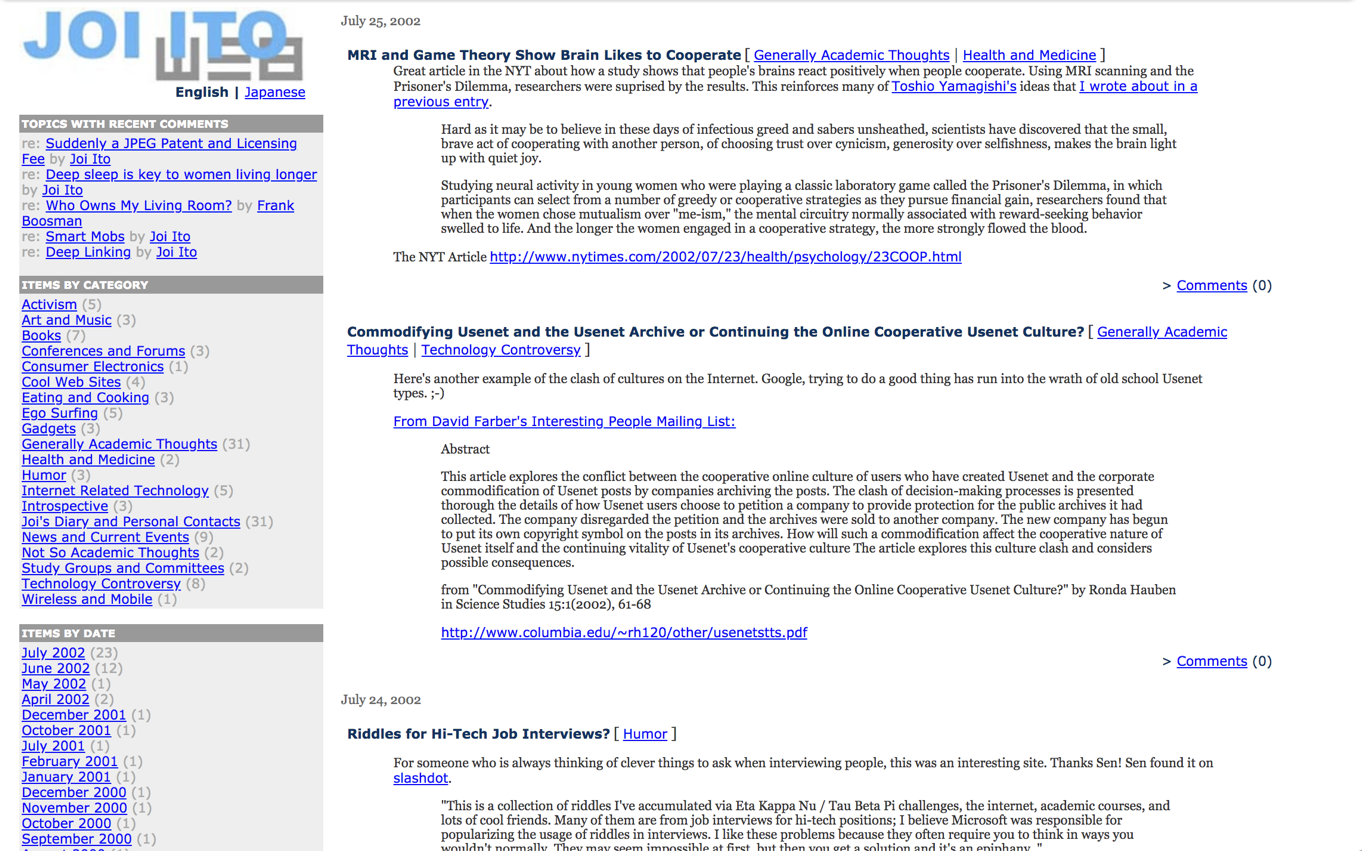
\includegraphics[width=1\textwidth]{pictures/joiblog}
 \caption{My blog in 2002.}
 \label{fig:joiblog}
\end{figure}

In 2002, I converted my personal website, which had a journal section, into a blog (see \autoref{fig:joiblog}) with the help of Justin Hall, who was arguably the first blogger on the Internet; he has been journaling at links.net since 1994. For my site, we used the blog software Movable Type and moved the journal entries from my personal website to the blog.

The big difference between the blog and my journal was that the blogging software made updating the website extremely easy. Posts could be written into a web interface instead of writing \ac{HTML} by hand, which I originally did, or using website design software such as Dreamweaver. Movable Type was open source and allowed plugins, and my team at Neoteny, led by Daiji Hirata, localized Movable Type for the Japanese context. We ended up investing in Movable Type and supporting it in Japan.

The fact that blog software was open source and that there was a community of blog software developers at the time were important factors in the rise of blogging. The community created open protocols like trackbacks, which allow blogs posts to receive the \ac{URL}s of blogs posts that link to them so that the linkbacks can be posted at the bottom of the blog posts. Most blog platforms and systems also allowed users to download all of their content and port it to another blog platform, a feature that was no longer available after the platforms became more commercial or were acquired by large companies.

Interestingly, Japan had had a long history of online journals, or ``nikki'' sites, and the community in Japan on sites such as 2chan attacked us quite vigorously because they believed that bringing blogs to Japan was unnecessary. This included a letter from the chairman of the \begin{CJK}{UTF8}{min}全日本電子日記協会\end{CJK} [All Japan Electronic Journal Association] complaining about the redundancy. I argued that the nikki sites weren't interoperable and that, in contrast, blogs were setting a global standard. I continued to be attacked until some of the standards we developed around blogging took off with the help of some larger companies that adopted them.

\subsubsection{RSS}

One example of a blogging related standard is \ac{RSS}. \ac{RSS} would eventually drive Google Reader and become the core way that many sites syndicated their content.

\ac{RSS} originally started at Netscape and was called \ac{RDF} Site Summary. This was version 0.9. After AOL acquired the company, Netscape dropped \ac{RSS} support from My.Netscape.Com and removed all documentation and tools. The \ac{RSS}-DEV Working Group produced \ac{RSS} 1.0, which reintroduced \ac{RDF} and added XML namespaces and metadata vocabularies -- in other words, making \ac{RSS} more complex and standard. David Winer, a blogger and the developer of the popular blog platform Radioland, then developed a version of \ac{RSS} in 2002 that was substantially simplified and called it \ac{RSS} 2.0, eventually renaming it ``Really Simple Syndication.''

Not surprisingly, this inspired a great deal of dispute and argument, with the \ac{RSS} 1.0 people arguing that \ac{RSS} needed to be extensible, robust and tied into other global standards. Dave and his \ac{RSS} 2.0 supporters argued that \ac{RSS} needed to be easy for developers and users to read and write to and that all of the complexity in \ac{RSS} 1.0 was unnecessary. This was only one of the many standards debates that occurred online at the time, but because of the emergence of blogging as a communications platform, we were able to have these debates on our blogs. 

I invested in and started working with a company called Technorati that aggregated blogs so that they could be searched --- Google was not yet paying attention to blogs -- and the links among them could be tracked. I also invested in a company called Blogrolling that built a tool that allowed bloggers to manage a list of their favorite blogs that would show up on the side of their own blogs. I also invested in a company called ECTO that allowed its clients to post to any blog platform that supported XML-RPC, a standard for programatically posting to blogs.

Through the conversations on my blog, experimenting with these standards myself, meetings that I attended or hosted,and nudging the companies that I invested in, I contributed to moving these standards forward. For example, in 2003, Ben Trott, the developer of Movable Type, and Dave Winer agreed to a standard change in the metaWeblog \ac{API} after a short exchange in the comments on my blog \cite{metaWebl87:online}. The way that we discussed these standards on our blogs became the basis for thinking about the future of online conversations.

\subsubsection{Emergence of Social Media}
\label{sec:emergentdemo}

I have a category on my blog called ``blogging about blogging.'' with over 500 entries. Through this process of arguing, fighting, agreeing, developing and becoming friends, we bloggers realized that a new kind of social network and governance system was emerging. The term ``emergent democracy'' was coined by Ross Mayfield, who was a member of our community. In 2003, I convened an online meeting --- a phone conference call --- where we discussed this phenomenon. The first call included Clay Shirky, Ross Mayfield, Pete Kaminski, Gen Kanai, Liz Lawley, and Sébastien Paquet, an impressive bunch. I wrote a first draft and then received input from the community on the paper in \autoref{emergentdemo} called ``Emergent Democracy'' which became the basis for a book called \emph{Extreme Democracy}. The final version of the paper is version 3.2 and is on my website \cite{1Emergen42:online} and an except is included in this dissertation in \autoref{emergentdemo}.

The paper contends that blogs were the first version of the phenomenon of online conversations that would change the way that democracy works. My hypothesis was that the current system of representative democracy in which we vote for representatives who deliberate and decide on policy on our behalf with the traditional news media reporting back to us is outdated. People can do more than vote: we could discuss and cause collective action directly through a self-organizing principle in the same way that the development of free and open source software had shown that we can collaborate without formal organizations. Clay Shirky calls this ``the power of organizing without organizations.'' The discussion and the paper itself were written in an emergent way, and it kicked off a movement to discuss and deploy means of governing ourselves through online communities.

In 2003, Howard Dean was a candidate in the Democratic primary in the United States, and I was invited to join the Dean campaign's Net Advisory Net, which offered advice about an online strategy for him. Many members of the network of bloggers were involved, and the Net helped pull off what was one of the first Internet driven political campaigns. I was quoted in Wired Magazine \cite{wolf2004internet} at the time, saying, ``You're not a leader, you're a place. You're like a park or a garden. If it's comfortable and cool, people are attracted. Deanspace [the Dean campaign's very early social network] is not really about Dean. It's about us.'' The campaign was really an online community. Even though the campaign was unsuccessful, its use of an online strategy and convening of an online community redefined the way political campaigns are conducted in the United States, as Joe Trippi wrote in a book about the experience, \textit{The Revolution Will Not Be Televised : Democracy, the Internet, and the Overthrow of Everything} \cite{trippi2004revolution}.

In retrospect, the paper ``Emergent Democracy'' was overly optimistic but nonetheless prescient about the fall of mainstream media and movements like the Arab Spring. When we wrote the paper, I believed the system would would figure out how to self-regulate and build another system more stable and better than the one that we had. I did not anticipate the inability of the revolutionaries of the Arab Spring to rebuild their countries or foresee issues such as so-called fake news. I also believed that conversations about democracy and governance would continue on decentralized systems and did not predict the power of platform companies like Facebook to centralize, aggregate and effectively mediate and control these conversations. I have also been surprised by our inability to contain anger, trolling, and hate speech on the Internet. Somehow I had hoped that once everyone was connected, we would all become friends.

I had my first experience with trolls when I set up a mailing list called ``Netsurf.'' I was working with \textit{Wired Japan} on its version of the Net Surf page of \textit{Wired} in the United States, which had Net Surf page from 1993 that listed interesting \ac{FTP} sites, Usenet newsgroups and email addresses. My Eccosys team set up a mailing list in February of 1995 to share links and talk about the Wired page. We ran the mailing list on our Sun SPARC 1+ and anyone in could join.

Although Netsurf began as a place to share new websites, it evolved into a virtual community where people came to talk about all kinds of topics online. At one point, a member began behaving in what I believed was an anti-social way, and so I told him that he needed to behave more respectfully and civilly. Since the mailing list was on my server and was the space was my virtual living room, I thought that members should follow my rules. But the members argued that the mailing list was a public space, and they didn't care what I said. I learned another lesson --- just because I ran the platform didn't mean I could control the conversation or the community.

As an aside, this was at the same time that ``Jerry and David's Guide to the World Wide Web,'' which turned into Yahoo! in 1994, was starting up, the Eccosys team was talking to Jerry Yang and David Filo about collaboration. We had agreed to do Yahoo! Japan with them, and the first time I met Jerry, he was asleep under a desk at Stanford University where they were getting started. Unfortunately, after I mentioned how exciting Yahoo! was in a conversation with Masayoshi Son of Softbank, he invested in Yahoo! and gained the rights for Yahoo! Japan for Softbank as part of the deal. Son-san asked us to set up Yahoo! Japan for Softbank, and I asked for fifty percent of the Yahoo! Japan business, which I thought was fair since we had originally thought we would have all of it before that. He agreed to give us about one percent of Yahoo! Japan. I told him that I'd rather be paid in cash, and we set up the beta version of Yahoo! Japan for him. Of course, I should have settled for the one percent he offered --- or maybe just kept my mouth shut instead of extolling the virtues of the company to him. But I learned a powerful lesson: investment and financial strength can sometimes outweigh relationships and technical ability.

When our discussions about emergent democracy began developing in earnest, we decided that we needed a real-time chat room to have a continuous conversation. I decided to set up an \ac{IRC} channel because it was open source and very accessible.

Remembering my failure to control my mailing list, I decided to call the channel \#joiito to make it very clear that it was my living room and not a public space. It became a hangout for hundreds of people interested in talking about emerging blogs and social software. Many influential developers hung out in the channel, and many software platforms were conceived and relationships forged there. Stewart Butterfield, who would go on to create Slack, was an active member of our community; Slack is based on \ac{IRC} and his experiences there.

Of course, there was the day that someone came to the channel and asked, ``So what does joiito think?'' After I answered, the person said, ``not you, the channel - \#joiito,'' and then I realized that I had just created another public space. It was called \#joiito.

\subsubsection{Online Communities and Online Learning}

The issue of civility and managing online communities has been one of my core interests and fields of experimentation. My interest in online communities dates back to my first experiences with bulletin board systems in the early 1980s and later services, such as NiftyServe, The MetaNet, Delphi, The WELL, The Source and CompuServe, where the message boards and conference areas were vibrant in content and relationships. In junior high and high school, these systems allowed me to interact with adults and learn through conversations rather than through struggling with textbooks. On The Source, I set up a conference area for every course I was taking in my senior year of high school and talked about the coursework with my friends online. This helped me understand the context of the topics and become more interested in them.

In my senior year of high school, I participated in a monthly meeting of what was called the RINGO Club, an Apple II users group of mostly Americans in Tokyo. I demoed to the group some of the online services I was using. I later started running a regular meeting called TNet, a gathering of the mostly English speaking local BBS and networking community. We shared tips about things like how to rewire the new Epson 300 baud modem to switch between Bell and CCITT so it would operate with US modems and tricks on how to get online. 

At a RINGO Club meeting, I met David Fisher, a retired U.S. Air Force pilot and English language teacher. at the International Education Center in Tokyo and its English language school, Nichibei Kaiwa Gakuin. He had a student named Toshiaki Tanaka, who was the president of a shrimp wholesaler and seafood retailer called Sakako Co., Ltd. Jeffrey Shapard, another English teacher at Nichibei Kaiwa Gakuin, was assigned to do research on educational technology together with Fisher. David connected Jeffrey with Mr. Tanaka and a programmer Tanaka had hired, Makoto Ezure, and they He put together a few entrepreneurial folks who came up with the idea for TWICS, an online communication system. TWICS, which stood for "Two Way Information and Communication System,” launched in 1984 as a system hacked to pick up a phone and connect it to a modem using two acoustic couplers and two Fujitsu personal computers because connecting modems directly to phone lines was still illegal in Japan.
% * <david@weinberger.org> 2018-07-05T19:53:08.975Z:
% 
% >  at the International Education Center in Tokyo and its English language school, Nichibei Kaiwa Gakuin. He had a student named Toshiaki Tanaka, who was the president of a shrimp wholesaler and seafood retailer called Sakako Co., Ltd. Jeffrey Shapard, another English teacher at Nichibei Kaiwa Gakuin, was assigned to do research on educational technology together with Fisher. David connected Jeffrey with Mr. Tanaka and a programmer Tanaka had hired, Makoto Ezure, and they 
% delete
% 
% ^.


When I came home after my first year in college, I spent the summer working on TWICS. We were trying to develop the service beyond a simple BBS. I became an advisor and a member of the TWICS team. 

By 1985, it became a multi-user system and was moved over to a MicroVAX. I pushed to get out of writing our own software and instead license existing software. We started running PARTI, which was the same conferencing system as The Source. TWICS became one of the first public services on X.25 and in 1990 joined JUNet as twics.co.jp. TWICS eventually became an important hub for experimenting with online communities in Japan.
% * <david@weinberger.org> 2018-07-05T19:55:32.949Z:
% 
% > TWICS became one of the first public services on X.25 and in 1990 joined JUNet as twics.co.jp. 
% delete?
% 
% ^.

I also met a number of researchers online who were experimenting with a service called the Electronic Information Exchange System (EIES). It was a multi-user online bulletin board system designed to deliver educational courses and provide a platform for research and communications. It was developed at the New Jersey Institute of Technology (NJIT), and I connected with some of the people doing the early work on it, including Murray Turoff.

In the fall of 1985, The New School offered the first set of fully online graduate courses for credit, and I took two courses, ``Artificial Intelligence \& Life'' and ``Propaganda: Lit Science.'' The propaganda course was taught by a former CIA officer, and the online conversations and content were fantastic --- I remember some of the lessons even today. What's notable about this, though, is that it was happening a decade before the Web and was a very sophisticated use of peer-learning and communities decades before people started talking about Massive Open Online Courses (MOOCs).

Lessons from my activities in communities like this class became the basis of my interest in and my theory of the role of community moderators, peer-learning and the importance of the structure for comments and threads for online discourse.

\subsubsection{Consolidation and Commercialization}

In 1995, Eccosys, my colleagues, Cyrus Shaoul, Sen Nagata, Jonathan Haggan, Hidetoshi Shimokawa, Daishi Harada, Yuki Nakayama and I set up a company for our Internet consulting business. We joined forces with an advertising agency subcontractor called From Garage, which was run by Kaoru Hayashi. We realized that although we dreamed of digital cash taking over the world, all of our income was coming through wire transfers of fiat currency from technology companies trying to promote their Internet products such as Novell Networks, Sun, IBM and others in Japan. At the time, my business skills were minimal and working together with a company that had been in business for more than a decade and knew how to sell services seemed like a good idea.

We worked with the \ac{WIDE} Project for the first time in 1995 on the World Jr. Summit funded by Isao Okawa of CSK. It aimed at connecting children from 40 countries via the Internet. We helped with the technology. That was when I first met Nicholas Negroponte from the MIT Media Lab, who was also working on the project.

That same year, we also built the first Internet cafe in Shibuya, which was sponsored by IBM to promote its new Internet native operating system, OS/2 Warp. The cafe was often the first place that young people without any technical know-how were able to experience the Internet first hand.

Jun Murai and I worked with Carl Malamud to plan and deploy the Internet World Expo in 1996. This was a large project that aimed to connect 80 countries and create online as well as real world pavilions to show people the Internet. Murai-san, the telecommunications companies and the \ac{WIDE} Project worked mostly on the infrastructure, and I focused on content and finding locations, like persuading Mori Buildings to help me create an Internet cafe in Laforet Harajuku.

After losing my shot to run Yahoo! Japan because of Softbank, I was contacted by Infoseek, a automated search engine portal in the United States that wanted my help localizing and launching Infoseek in Japan.

Yahoo!, Infoseek and others had realized  that as personal web pages proliferated, just reading the Netsurf column in \textit{Wired} wasn't enough to keep up with all of the interesting things going on. Even Yahoo! began to have a hard time keeping track of new websites. We realized that a search engine that crawled the Internet, traversing links and finding new websites to create an automatic directory was possibly a key innovation. The theory of ``the portal'' as a consolidated place that would monopolize attention began to take shape.

In 1996, two years before Google was founded, we were using OMRON's SuperMorph-J to do the first ``word breaking''\footnote{Japanese language doesn't use spaces and there is no obviously way to figure out the beginning of a word and the end of a word. This is confounding to search engines. For instance, the name \begin{CJK}{UTF8}{min}山本\end{CJK} [Yamamoto] is two characters, \begin{CJK}{UTF8}{min}山\end{CJK} which means ``mountain'' and \begin{CJK}{UTF8}{min}本\end{CJK} [moto] which means ``root.'' When you search for \begin{CJK}{UTF8}{min}山本\end{CJK} [Yamamoto] you want to find all of the \begin{CJK}{UTF8}{min}山本\end{CJK} [Yamamoto], not every article on mountains along with all of the results for root. A word breaker parses a Japanese sentence, figures out where the word breaks are, and indexes and searches for words rather than characters.} to increase the quality of search.

 Many portals like Yahoo! and Infoseek in the United States had begun to believe that search wasn't as important as offering an array of services such as email, chat, sports and .news. They began to deemphasize search. 

In Japan, Yahoo! and other websites sold advertising in the same way that magazines sold advertising, by a sponsor for a section for a period of time. They would measure how many people saw the advertising, but the advertiser for any page was always the same at any given time. In the United States, Infoseek and others had begun ``rotating'' advertisements and selling advertising by the number of views.

Japanese advertisers and advertising agencies were very much against this method. They didn't like the idea that their advertising might be sharing a page with a competitor. They also didn't like the new way of measuring and selling advertising. Since the advertising agencies were so opposed, we worked with the Kokokunushi Kyokai, the trade group representing advertisers, to run a series of studies and working groups to experiment with --- and get advertisers comfortable --- with the idea of rotating banner ads.

After winning over the advertisers, we worked with a consortium --- Hakuhodo, Asatsu, Yomiko, I\&S and Tokuma Shoten --- to create an ad representation company called the Digital Advertising Consortium (DAC) to initially sell advertising on Infoseek and other websites using this method.

This was the beginning of commercialization of the Internet; the beginning of the advertising driven model for content in Japan, and also the creation of the first ``platforms'' or ``portals.'' Google and search would eventually win over the curated ``network of services'' portals, and simple ad rotations purchased on websites would become a small business compared to adwords and programmatic ad buying.

Blogs would emerge, fueled in part by the search engines pushing traffic to the edges of the Internet. We had long debates about ``the long tail,'' the argument that the lower cost of publishing and distribution would mean only minimal traffic would be needed to support very minor websites. Clay Shirky disagreed, insisting that a power law meant the top sites would become more dominant.

In many ways, he was right, and the decentralized blogging of my youth gave way to the emergence of social media, which changed the architecture from search engines and blogs to centralized platforms.

\subsubsection{Twitter}

In the early days of blogging, Blogger, a blog software platform, was major player in the market. I had been talking to Ev Williams, its CEO, and was trying to develop a relationship with him. I had just offered to invest in Blogger and sent him a term sheet when I learned that the company had been acquired by Google. But I kept in touch with Williams and the rest of the Blogger team, and we remained friends.

Blogger didn't flourish inside of Google and slowly the team left. Williams started working on new ideas, including audio blogs with Noah Glass in a company called Odeo. I was interested in this space, having worked with Nokia and others on multimedia, including being early in setting up mobile blogging or Moblogs. Boris Anthony, who did the design and user interface work on my blog, and Adrian Tijsseling, the creator of Ecto, a system that allowed you to post to blogs from a client, worked together to make make many of the early tools for mobile blogging. At Odeo, they started working on Twitter as an idea for mobile blogging using SMS.

I was intrigued and became an early user. Twitter was clever and created an \ac{API} to allow developers to connect to Twitter, and even though Twitter didn't support Japanese well, many Japanese developers created tools for Twitter. I reached out to Williams and together with Kazuya Minami and Hiroki Eda of Digital Garage, we localized and launched Twitter in Japan. This was early days for Twitter and because Digital Garage had experience selling advertising, we were able to launch a version of Twitter in Japan with advertising even though Twitter in the United States had no advertising at the time.

Digital Garage invested in Twitter and incubated the Japan operations in our offices through a partnership in 2008. Twitter was exciting for me because it was a social hub that sent traffic to blogs and other websites, so it seemed like an interesting and social alternative to search engines. Initially, Twitter appeared to be a great place to have casual conversations about your day and share links with your friends. We didn't realize that Twitter would become the conversation itself, or that the short form of a Tweet, just 140 characters, was more suitable and convenient for people to post content than the longer format of blogs. Twitter also would eventually capture most of the traffic from blog comments, which had been an important part of a blog community. 

\subsubsection{}{Helping Main Stream Media}

The assault on the main stream media that I helped fuel through fighting on the blogger's side of the battle between the amateur press and the professional press was unexpectedly successful. This was only partly due to the quality of the citizen journalism and probably more as a result of the deteriorating business model of mainstream media. Craig's List and other web-based businesses destroyed first the classified ads as a major revenue source. The Internet platforms and online advertising continue to grind away at ad revenues. And while people laughed at Media Lab founder Nicholas Negroponte when he, in the 1990s, suggested that we would be reading news over the Internet, print advertising continues to decline.

As I began to see the demise of main stream media, I joined the board of trustees of the John S. and James L. Knight Foundation in 2011. The Knight Foundation, started by the Knight brothers who ran a US nationwide network of newspapers, created the foundation to engage and inform communities. The foundation focuses a great deal of its efforts in supporting journalism. Through the board, I have contributed to the foundation's support of new business models, understanding the role of social media and investigating the impact of \ac{AI} in the future of the public sphere.

In 2012, I joined the board directors of the \textit{New York Times} and continue to participate actively in the board. The New York Times is one of the few newspapers that has successfully made a transition to a sustainable online subscription model and is constantly exploring new business models and forms of journalism. Through my participation on the board, I have learned a great deal about the business of professional journalism as well as contributed my experience in building and participating in online communities and the creation of content online.

\subsubsection{The Media Lab and the Public Sphere}

Since joining the Media Lab, I have been involved in its Center for Civic Media. The center is run by Ethan Zuckerman, who has been working to understand the public sphere in the digital age and how to interact with it. Media Cloud, a project his group developed together with the Berkman Klein Center for the Internet \& Society at Harvard University, is an excellent example of a tool that can examine how conversations on blogs and media online occur. It lets researchers track ideas and phrases as they move through the mainstream and blog-based channels of the Internet. By looking at such patterns online, Zuckerman and his colleagues can see how communities and news interact to shape the way issues develop in the media.

In their study, ``Breitbart-led right-wing media ecosystem altered broader media agenda'' \cite{benkler2017study}, Zuckerman and his colleagues used Media Cloud to study over 1.25 million stories published online between April 1, 2015, and Election Day. They analyzed ``hyperlinking patterns, social media sharing patterns on Facebook and Twitter, and topic and language patterns'' published by 25,000 sources. ``When we map media sources this way, we see that Breitbart became the center of a distinct right-wing media ecosystem, surrounded by Fox News, the Daily Caller, the Gateway Pundit, the Washington Examiner, Infowars, Conservative Treehouse, and Truthfeed.'' See \autoref{fig:twittermediacloud}.

\begin{figure}[h]
 \centering
 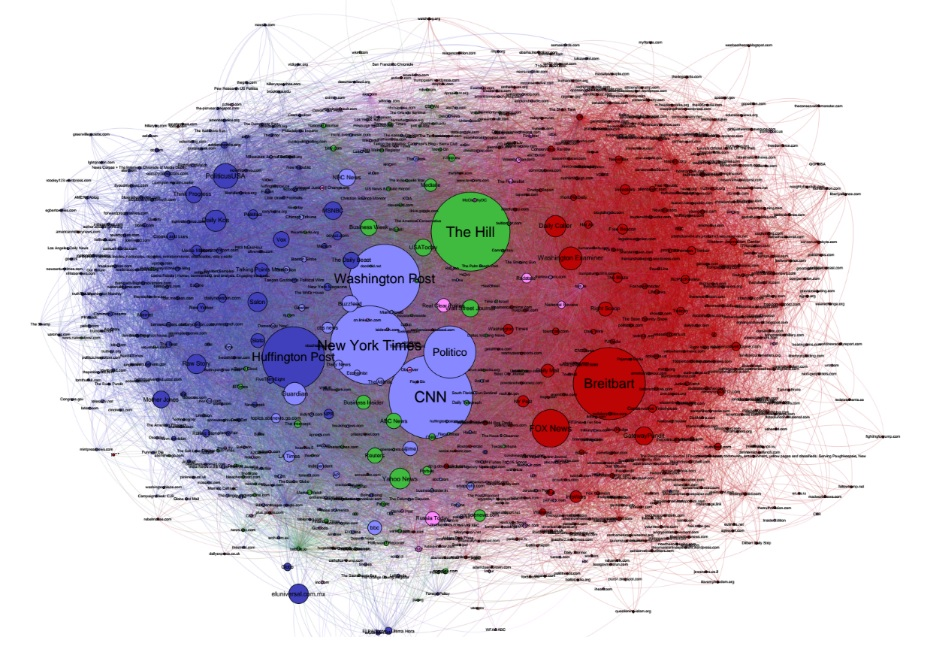
\includegraphics[width=1\textwidth]{pictures/Twitter-Image-1}
 \caption[Media sources shared on Twitter during the election]{Media sources shared on Twitter during the election. (Nodes sized in proportion to Twitter shares. Source: Center for Civic Media at the Media Lab.)}
 \label{fig:twittermediacloud}
\end{figure}

Another group at the Media Lab, the Laboratory for Social Machines run by Deb Roy, deployed the the Electome project \cite{Enterthe97:online} in the 2016 election to look at how supporters of various candidates were connected to each other on Twitter and what they were talking about \cite{electome:online}. Their research revealed how polarized and disconnected these communities were. By mapping the ``tribal networks'' of Twitter users during the elections, as well as some 30,000 journalists on Twitter. they found that almost none of the journalists were in the ``Trump tribe.'' (See \autoref{fig:electome})

\begin{figure}[h]
 \centering
 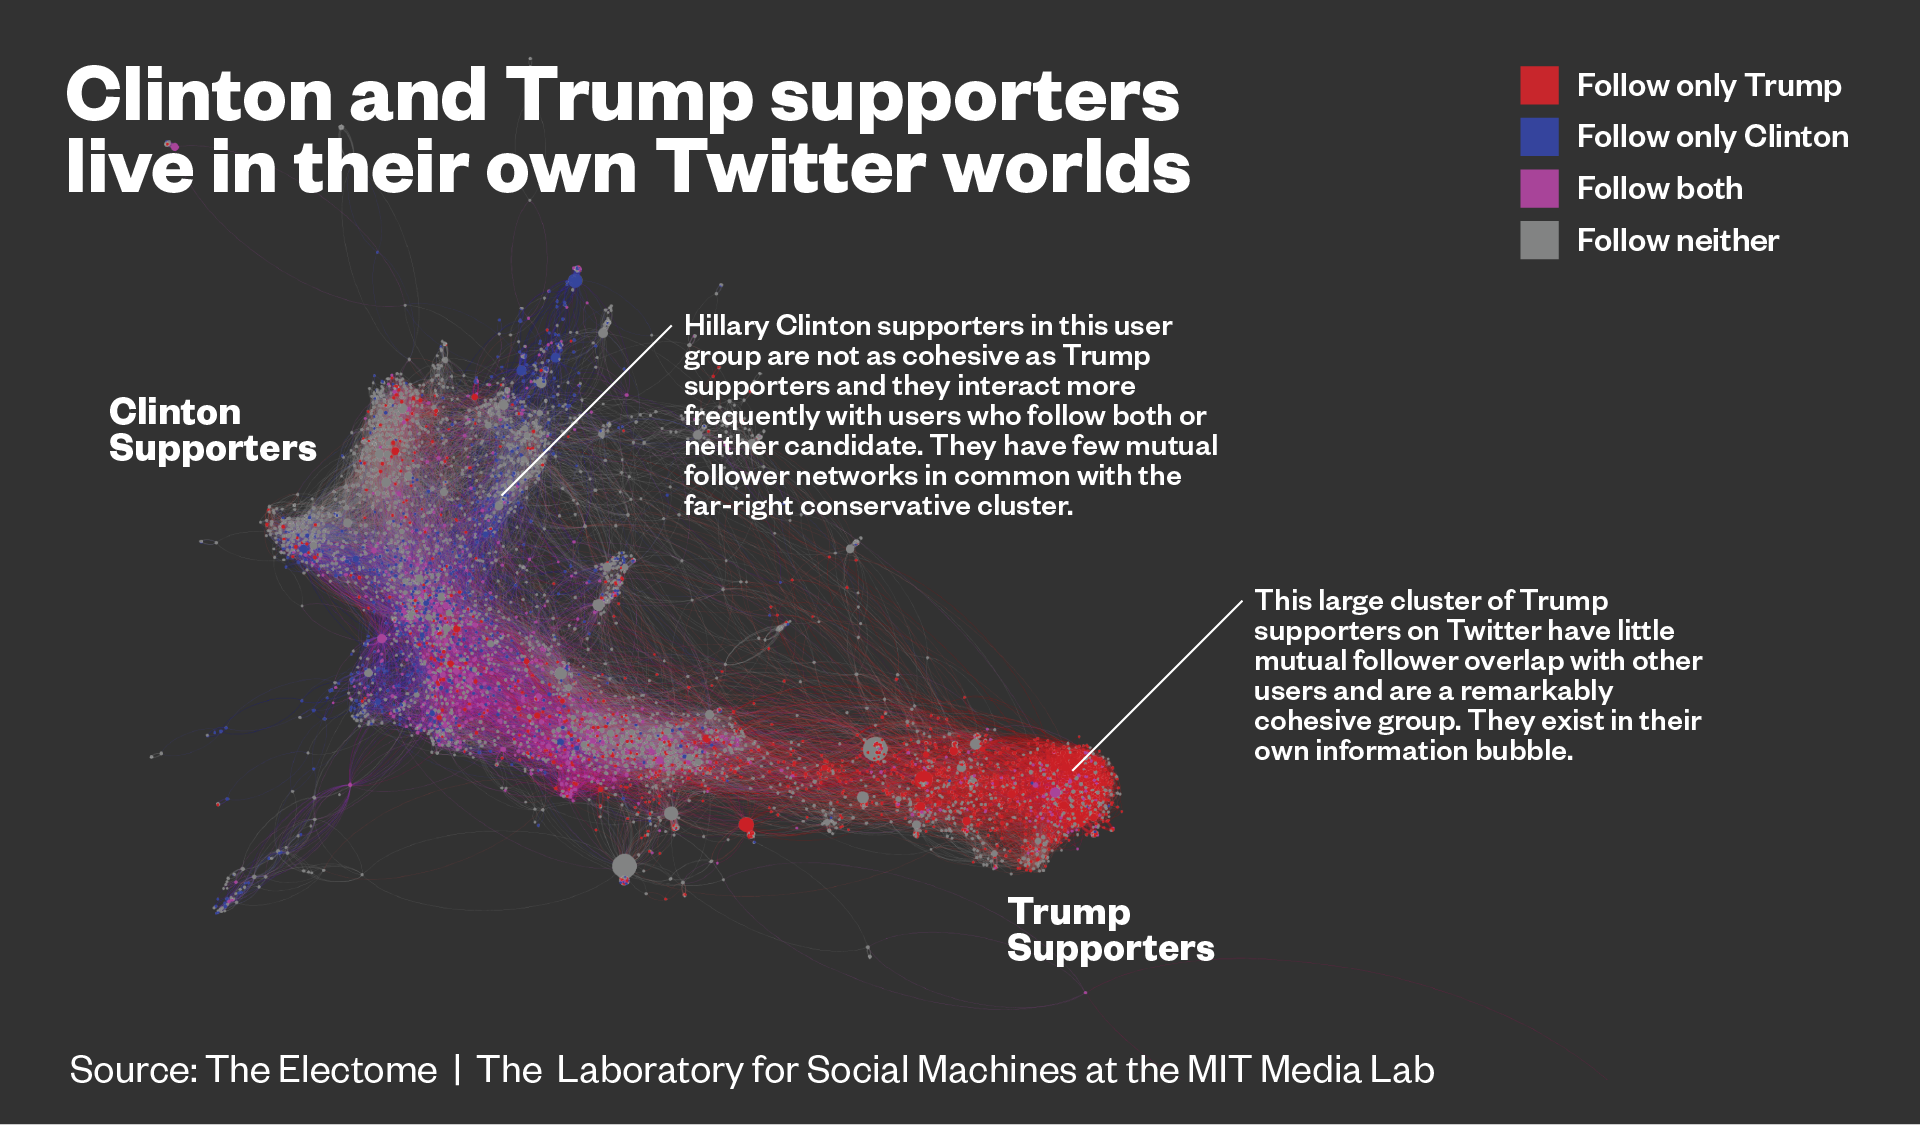
\includegraphics[width=1\textwidth]{pictures/TwitterData1-01}
 \caption[Clinton and Trump supporters live in their own Twitter worlds]{Clinton and Trump supporters live in their own Twitter worlds. Source: The Electome - The Laboratory for Social Machines at the MIT Media Lab.}
 \label{fig:electome}
\end{figure}

In another project, Roy's group has analyzed 11 years of Twitter data to examine the dissemination of rumors as defined by a number of fact-checking sites . The research showed that false rumors spread differently and more quickly  than true stories  do\cite{vosoughi2018spread}. They are also able to show the shape and relationships of the networks of people discussing any issue online. When they analyzed replies to tweets about stories to figure out the emotional response to those stories, they found that ``surprise'' and ``disgust'' were far more often expressed in response to false stories than true stories. This suggests (but does not prove) that in-the-moment emotional response may be a causal factor in why people share stories that turned out to be false. (It also is easier to write a surprising story if it doesn't have to be true.)

Roy's group has  begun to measure shared reality and the civility of the conversations online across different ``tribes'.'  They are also developing public sphere health metrics in a non-profit spin-out from the Lab called Cortico \cite{Cortico96:online}. Cortico is  building tools for local journalists and community organizations to help rebuild community communication, especially in news deserts.

\section{Technology for Social Justice}

\subsection{Artificial Intelligence}

\subsubsection{Ethics and Governance in Artificial Intelligence}
\label{sec:EGAI}

\textbf{Regulatory systems for \ac{AI}}

\marginpar{Our challenge today --- right now --- is to come up with methods to design, audit, and manage the development and the deployment of these systems so that they are socially beneficial.}Watching artificial intelligence and machine learning being developed and deployed so rapidly brings back feelings of watching (and participating in) the Internet in the early 1990s. AI could have an even bigger effect on society than the Internet. But, unlike the Internet it does not appear to be unbundling, or layering, itself. This is a significant issue because while the Internet by its nature was open to users, and derived its value from what users added to it, most AI system are being designed by computer scientists. These systems' effectiveness and bias are determined by the data chosen by computer scientists, and the training and optimization decisions made by them.

Because machine learning systems are trained by providing them with existing data, and because that data almost inevitably reflects existing human biases,  these systems often reinforce those underlying biases. In addition, it is to use the output of AI in inappropriate ways.

Our challenge today --- right now --- is to come up with methods to design, audit, and manage the development and the deployment of these systems so that they are socially beneficial.

I have been engaged in a number of efforts to try to support the introduction of ethics and governance in the development of \ac{AI}.

\textbf{Course on the Ethics and Governance of \ac{AI}}

Harvard Law Professor Jonathan Zittrain and I teach a course on the Ethics and Governance of \ac{AI} \cite{TheEthic48:online}. The course brings students from MIT and Harvard together from disciplines including law, engineering, philosophy, policy, history, and others. The course engages the class in readings, projects and a dialogue around the issues raised by \ac{AI}, as well as thinking about possible solutions.

The key motivation for the course is to try to teach social scientists about engineering, and \ac{AI} and the engineers about the social sciences and \ac{AI}. The course description is:

\textit{This course will pursue a cross-disciplinary investigation of the implications of emerging technologies, with an emphasis on the development and deployment of artificial intelligence. We will cover a variety of issues, including the complex interaction between governance organizations and sovereign states, the proliferation of algorithmic decision making, autonomous systems, machine learning and explanation, the search for balance between regulation and innovation, and the effects of \ac{AI} on the dissemination of information, along with questions related to individual rights, discrimination, and architectures of control. The course will entail an intense array of learning and teaching methods. Students will be expected to participate in a variety of activities. The class may include Media Lab and Berkman Klein Center fellows and affiliates.}

So far, we have been quite successful. A number of engineering students have gone on to become fellows at the Berkman Klein Center and even been admitted to the Harvard Law School. My hypothesis for now is that it's easier to get engineering students interested in a law degree than law students interested in an engineering degree. In any case, the creation of people proficient in both law and engineering is essential for bridging the gap and creating truly creative solutions. However, its likely that we might need a new joint degree program since getting a three-year Juris Doctor (JD) in Law after a degree in engineering seems excessive if the student doesn't actually want to become a lawyer.

The student surveys have made clear the difficultly of having a cross-disciplinary class. Because the class includes law students, philosophy students, computer science students and others, the class has to be accessible to people from other disciplines and necessarily feels shallow to some of them. We should probably experiment with different structures, such as having breakouts to go deep, or to do primers for novices. Another idea would be to have smaller out-of-class dinners or extended office hours to allow some students to go deeper.

Running a cross-disciplinary class in a new area will continue to be a challenge. I hope  we can improve and learn from others.

Together with the course, we have run a program called the \href{https://cyber.harvard.edu/research/assembly}{Assembly}, which brings professionals from industry, academia, government and other sectors to work in teams on  real projects involved \ac{AI}. These ``assemblers'' also participate in the class.

\textbf{The Ethics and Governance of \ac{AI} Fund}

Together with Reid Hoffman, Jonathan Zittrain and Alberto Ibarguen, we have raised a \$26 million fund to support research on the ethics and governance of artificial intelligence. The projects are at the Media Lab, the Berkman Klein Center (where I  have an appointment), and other third-party institutions.

One key design is for teams to work together on projects in an integrated way. The MIT Media Lab and the Berkman Klein Center are the anchor institutions where the largest portion of the funding is directed. We are also directing funding to other organizations that will work closely with us on our key themes. 

We are  uniquely focused on theory and deployment in the real world. The project's work is in three main areas:

\begin{enumerate}
\item Kinetic autonomy --- autonomous vehicles and weapons.
\item Algorithmic justice --- the use of algorithms in social systems such as criminal justice, housing, and insurance, with a focus on bias and the  positive uses of algorithms to improve society.
\item Information veracity --- with the emergence of platforms fueled by targeted advertising and content optimization, we have seen a deterioration of the quality of information and an increase in the influence by outside governments and businesses. What are the problems and solutions?
\end{enumerate}

I am personally deeply involved in the Humanizing \ac{AI} in Law project, which is supported by the fund. We are working to understand the risks of using algorithms in criminal justice, such as using them to generate risk assessments for pre-trial bail. I am also working to use algorithms to understand underlying causal relationships and address systemic problems, rather than just improving the predictive accuracy of algorithms.

\subsubsection{Humanizing Law in \ac{AI} (HAL)}
\label{sec:HAL}

Together with my group, Chelsea Barabas, Karthik Dinakar and Madars Virza, I am engaged in a number of activities including the publication of papers such as ``Interventions over Predictions'' for \textit{Fairness, Accountability and Transparency conference} in \cite{barabas_interventions_nodate} and two letters to the Massachusetts Legislature on pre-trial risk in \autoref{appendix:A} and \autoref{appendix:B}. More recently, I have written the following article for \emph{Wired} about the topic \cite{ItoWiredAI}, and I am speaking a great deal about this.

\textbf{The Church of Prediction and Solutionism}

\begin{quote}
\textbf{When it comes to \ac{AI}, we don't need crystal balls. We need mirrors.}\footnote{Draft of a more academic version of an article written for \emph{Wired}. The final version is available online \cite{ItoWiredAI}.}
 
Critics of artificial intelligence have pointed out the myriad ways that bias distorts the categorizations and predictions generated by algorithms. In response to these concerns, many computer scientists have tried to sanitize their predictive models by identifying and removing ``proxies'' for sensitive social categories like race, in an effort to curb the discriminatory effects of their tools. 

But this colorblind approach to fairness has some serious pitfalls, especially when it comes to addressing the needs of our society's most marginalized populations. For these groups, the core issue surrounding \ac{AI}-enabled decision making is not so much one of accurate prediction and bias, but rather, one of self-determination and social inclusion.
 
This is a topic that my colleague Chelsea Barabas discussed at length at the recent conference on Fairness, Accountability, and Transparency, where she presented our paper, ``Interventions Over Predictions: Reframing the Ethical Debate for Actuarial Risk Assessment.'' (See \autoref{appendix:C} for the full text of the paper.) In that paper, we argue that the technical community has been evaluating the ethical stakes of \ac{AI}-enabled technologies with the wrong measuring stick. By narrowly framing the risks and benefits of artificial intelligence in terms of bias and accuracy, we've overlooked more fundamental questions about how the introduction of automation, profiling software and predictive models connect to socially desirable outcomes.
 
This is perhaps most clearly illustrated in the realm of criminal justice reform, where a variety of predictive technologies are being used to assess and inform the management of ``risk.'' Reformers from across the political spectrum have touted risk assessments as a more objective means of making a wide range of decisions, from sentencing to probation and parole. Yet a 2016 ProPublica \cite{angwin2016machine} investigation revealed that not only were these risk assessments often inaccurate, but the cost of that inaccuracy was borne disproportionately by African-American defendants, who were almost twice as likely to be labeled high-risk but not actually go on to commit subsequent crimes. 

This report sparked a flurry of debate, much of which has focused on the inherent trade-offs \cite{kleinberg2016inherent} of designing a tool that uses imperfect data to make its predictions. To get a more complete picture of the costs and benefits of \ac{AI}-enabled tools like risk assessment, we have to zoom out to understand how these tools shape the outcomes that the criminal justice system is designed to achieve. This requires looking beyond issues of predictive accuracy, to understand how these tools serve as the basis for intervention in people's lives. 
 
In the case of pretrial risk assessment, that means asking deeper questions about how such assessments support certain ways of interacting with individuals awaiting trial. Pretrial risk assessments have become a major vehicle for bail reform in states like New Jersey and Kentucky, where they are implemented as part of a broader effort to minimize the use of a cash-based bail. Multiple studies have shown that cash bail as a pretrial condition is not only ineffective, but deeply punitive \cite{lum2017causal,heaton2017downstream}. In many cases, cash bail is effectively used as a means of detaining defendants and denying them one of their most basic rights, the right to liberty under the presumption of innocence. 
 
Nonetheless, critics of risk assessment are concerned that efforts to reform cash bail will inevitably lead to a significant expansion of non-monetary conditions, such as electronic monitoring and mandatory drug testing. Community organizations like the Chicago Community Bond Fund have started to track the adverse consequences of such non-cash bail conditions \cite{pretrial36:online}. This sort of community-driven oversight and research is absolutely critical because it helps us understand whether or not replacing cash bail with other types of conditions is in fact simply substituting one excessively punitive measure with another. 

That is the risk that we run if we introduce algorithmic predictions into a complex system without incorporating an informed understanding of effective intervention.
 
Such issues are not limited to the realm of the criminal justice system. In her latest book, \textit{Automating Inequality} \cite{eubanks2018automating}, Virginia Eubanks describes a number of compelling examples of failed attempts by state and local governments to implement automated decision making technology, such as a screening software for welfare benefits and housing, in an effort to deliver social services more efficiently and effectively. Eubanks details the use of data by the Office of Children, Youth and Families in Allegheny County, Pennsylvania, to screen calls and assign risk scores to families to help decide whether case workers should intervene to ensure the welfare of the child.
 
Three-quarters of cases that come through the office arrive because some public official has determined that a child has suffered ``neglect'' rather than abuse --- meaning that the symptoms of a high-risk child really look a lot like the symptoms of poverty \cite{eubanks2018automating}. This is partly because the majority of the data used to train the office's algorithm comes from public agencies, where data is collected whenever someone taps low-cost or free public services, such as drug rehabilitation or mental health treatment. Based on these risk factors, a child could be removed from her home and placed into the custody of the State, where her outcomes look quite bleak. Children who ``age out'' of the foster care system are significantly more likely to struggle with unemployment, homelessness, chronic illness and the law \cite{reilly2003transition, courtney1998foster}.
 
Rather than using predictive algorithms to punish low-income families by removing their children from their homes, Eubanks argues, we should be using data and algorithms to ask better questions about which interventions will be most effective in stabilizing a child's homelife by addressing the underlying drivers of poverty that exist in her life. 
 
These examples point to the fact that, in essence, we've been trying to use algorithms to develop a crystal ball to look into the future of some of society's most ``risky'' individuals when, in fact, what we need is a mirror to examine ourselves and our social systems more critically. We need to understand the underlying causes of crime and poverty, rather than simply using regression models and machine learning to punish people in high risk situations.

\marginpar{We must use algorithms to provide tools for reflection and self-awareness and improve the condition of society with civic engagement and participant design, or systems are designed by their participants.}That's exactly what researchers in the Media Lab's Humanizing \ac{AI} in Law are working on. They are asking questions that aim to get at the underlying factors that shape behavior the courts care about, such as the failure to appear for a hearing. Right now, the concept of ``failure to appear'' as a risk category is very general: people who skip town are clumped together with the much larger number of individuals who simply have logistical challenges in making their court date. Many of those challenges are related to poverty: a lack of reliable transportation or childcare, inflexible work schedules, or other family emergencies. If the courts want to be serious about reducing the number of people who fail to appear, then they need to engage with research around these issues to identify and rigorously test interventions that address those problems. 
 
We will also study the effects of policies like drug testing as a condition of release. As I mentioned above, these sorts of conditions are being widely used without truly understanding their effectiveness against recidivism, and more importantly, on the overall health of a community --- its crime rates, jobs, the health of its denizens. By incorporating transparency and community participation in the design of algorithms, the public and the fiduciaries can guide agencies using these algorithms to focus on the bigger picture \cite{balkin2015information}. The use of algorithms to help administer public services presents either an amazing opportunity to design effective social interventions or a tremendous risk of locking in existing social inequity.
 
To avoid the threat and seize the opportunity, we must reframe the debate and move from ``unbiased'' prediction to understanding causal relationships.
 
Algorithms trained to make predictions, by definition, use statistics and data to anticipate events so that risks are reduced or gains increased. When used in systems like forecasting the weather, they increase societal value, generally speaking. But when prediction is used against vulnerable people, we enable the transfer of freedom and agency from the disadvantaged to those in power. This is at odds with the fundamental premise of democracy.

Of course, using algorithms and data to understand causal, rather than predictive, relationships is not a silver bullet solution. The problems that we deal with are modern versions of the problems that have plagued society since the very beginning --- income disparity, xenophobia, exploitation, human bias. We must use algorithms to provide tools for reflection and self-awareness and improve the condition of society with civic engagement and participant design, or systems are designed by their participants.
\end{quote}

The key point of this article is the shift to causal inference away from purely predictive correlations. This will be key in applying machine learning to the complex systems and communities that we are trying to understand and intervene in. \textit{The Book of Why} by Judea Pearl and Dana Mackenzie that came out on May 1, 2018 describes what they authors call the ``causal revolution'' and describes the way in which statistics has stifled the study of causality --- the key to understanding systems and interventions \cite{TheBooko68:online}.

\subsection{Health}
\subsubsection{Principles in Awareness}
\label{section:awareness}

For the last four years, I have been teaching a course called Principles of Awareness with The Venerable Tenzin Priyadarshi.

Following is the course description: \\

\textbf{Description}

\textit{What is awareness? Is it a ``default'' state or is it cultivated? Can it improve performance and wellbeing? What role does technology play in promoting or hindering awareness? Is there an ethical framework for our capacity to be aware? And can self-awareness be linked to happiness? The course will be set in an experiential learning environment where students will explore various theories and methodologies around these questions. Students will be required to keep an open lab book documenting their observations, and present them regularly during class sessions. The final project will consist of evaluating and developing awareness tools, techniques and interfaces targeted towards performance and wellbeing.} \\

\textit{Themes to explore}
\begin{enumerate}
\item \textit{Boundaries of Awareness: Self and Other}
\item \textit{Change}
\item \textit{Relational Awareness}
\item \textit{Non-Duality}
\item \textit{Joy and Happiness}
\end{enumerate}

\marginpar{in, out\\
deep, slow\\
calm, ease\\
smile, release\\
present moment, wonderful moment\\
--- Thich Nhat Hanh}
\textit{Class meetings will consist of practice, lectures and discussions with invited speakers. Some of the talks will be open to the public. And the practice will range from meditation to hacking.}

The course engages our students in a deep exploration that helps them better understand their intrinsic motivations and become aware of their previous conditioning, as well as to think about questions about health, motivations, emotions and goals. The course requires students to sleep 7-8 hours a day, keep a regular meditation practice and ``notice one new thing per day.'' Through this practice and conversations in class, we explore the theory and practice of becoming aware.

I believe that awareness and the exploration of intrinsic motivations through contemplative practice is an essential component of a healthy mind, culture and body, and through this course, I cultivate this practice in myself as well as support students in their development and exploration. Student journals are posted on \href{https://awareness.pubpub.org/}{our website}. We just completed the class for the fourth year, and now a dynamic community of alumni is beginning to form, a community with a culture of intrinsic motivation, awareness and new notions of flourishing.

\subsubsection{Health 0.0 Project at the Media Lab}
\label{sec:health00}

\textbf{Overview}

There are massive gaps in developing and using key emerging technologies and tools in pharma, biotech and health member companies at the Media Lab. The Media Lab can provide a suite of tools for these needs and co-develop new ones that do not exist.

The Media Lab can catalyze novel and unorthodox interactions, hypotheses and breakthroughs by convening and conducting research with leading researchers working at MIT and other institutions on health. It can serve as a neutral convening venue for top pharmaceutical and health companies, as well as leading foundations and technology companies. Dr. \href{https://www.pratiks.info/}{Pratik Shah} is working with faculty, researchers, and me on the research, managing and documenting the discussions and research and publishing papers.

Additionally, the Media Lab and its members can co-design hypothesis-driven questions and novel research projects with tools and access to data. One of the outputs will be fundamentally new knowledge of health processes that will lead toward a real-world impact on preclinical discovery, clinical trials, clinical development in patients, and point-of-care technologies.\\

\textbf{Theory}

We plan to work with experts  in fields that historically have not worked together in the hope of developing unorthodox hypotheses and intellectual and scientific breakthroughs. We will engender and provoke antidisciplinary interactions between biology, clinical medicine, computer science, and the mathematical and physical sciences to generate breakthroughs in solving grand challenges and create new research opportunities to leapfrog existing approaches. We will build trust to openly discuss issues across disciplines. Questioning assumptions on ground truth about fundamental processes will allow us to develop theoretical and practical systems to model and understand the human body. We will also develop new theories for diagnostics.

The development of theory also generates novel models for human health and medicine (systems level vs pathways, microbiome, music, meditation, relaxation, etc) that may have prognostic value but have not been explored or do not have business models. This will lead to new paradigms for health care. \\

\textbf{Brainstorming}

A select group of experts from a variety of different fields in physical, chemical, biological, and computational sciences met at the Media Lab on January 18, 2018, for the Blue Sky Drug Discovery Workshop with GlaxoSmithKline, the drug company, and John Baldoni, a senior researcher at GSK. This was a typical Media Lab-type brainstorming session with no presentations or official panels or talks. The focus was simply ``The Future of Drug/Therapeutic Discovery.'' It was a rare chance for people from a variety of disciplines to get together and discuss what they would like to see happen in drug and therapeutic discovery. The workshop did not start with a presentation of anyone's current research, but rather discussed the current state of health research and various avenues of interest of the participants. \\

\textbf{Practice}

The development practice brings together leaders from academia, industry, and government to solve ``here and now'' issues in the  discovery and research and clinical development process. This engenders the integration, development and impact of key enabling tools (AI, cryptography, CRISPR, etc.) We work with data, problem statements and opportunities brought to the Media Lab by the Food and Drug Administration (FDA), the National Institutes of Health, the National Cancer Institute and pharma, biotech, and member companies, as well as other academic collaborators and foundations. This will lead to rapid benefits and improve health research: safer and faster clinical trials; digitally empowered researchers, clinicians, regulators and patients, and reducing health care costs. \\

\textbf{Execution and Considerations}

Pharma and health companies often do not benefit from creative and cutting edge research done in top tier universities and end up licensing enterprise solutions from corporations, which often demand large amounts of data, do not share algorithms, and demand a share of intellectual property.

Academic research universities have students searching for exciting research projects, and health data can play a vital role in training them if it becomes readily available. Currently it is not. The project aims to integrate the massive amounts of publicly available clinical trial data from FDA and other sources to build models and algorithms. The Health 0.0 project is convening and supporting researchers and institutions in the acquiring, sharing, discussion and analysis of case studies, publications and concrete examples of types of biomedical, preclinical and clinical data, their preferred format, structure and amounts usually generated by proprietary pharmaceutical industry projects, research institutions. Some are publicly available via \href{https://clinicaltrials.gov/}{clinical.trials.gov} etc. The project investigates how they are currently being analyzed using Bayesian modeling, statistics, bioinformatics, and systems biology.

As we pursue these opportunities, it will be important to share with member companies the current state of machine learning and \ac{AI} in computer science, CRISPR, gene editing and other technologies. We are conducting biannual workshops on these topics. Examples of core capabilities, applications and new architectures of \ac{AI} (\ac{DNN} and other models), types of data they can process and classify will also be discussed and evaluated. \\

\textbf{The \ac{AI} Example}

Almost all \ac{AI} classification, prediction and learning architectures today are being developed using non-clinical datasets that are abundant in size and often well-annotated. Over the past few years, progress has been made in developing deep neural network (DNN) architectures that can learn from fewer examples (low-shot learning); can make sequential and logical deductions using sparse temporal data (recurrent neural networks); learn sequential policies with minimal supervision (reinforcement learning (RL)), and generative adversarial networks (GANs) that can generate synthetic data to augment sparse datasets. These new approaches hold promise but must be substantially modified to accept clinical datasets that often do not perform with the same efficacy as non-clinical data. 

We need to make health data accessible, labeled, structured and organized to make it useful. 

The ability to track intellectual property contributions in joint research projects is important. Additionally, a layered silicon semiconductor approach could be useful.

The Health 0.0 project will also engage in brainstorming sessions to identify opportunities to use \ac{AI} and machine learning to solve specific problem statements from each organization. For example: For a particular problem statement, do you have access to the data? Is it structured for machine learning? How many data sets are needed and for what outcomes?

We will develop case studies, publications and concrete examples of Media Lab groups, startup companies (eg: Benevolent \ac{AI}, Deepmind, Good \ac{AI}, Vicarious, etc.) and foundations that have developed \ac{AI} architectures for analyzing clinical data.

We will also develop value propositions supporting building a horizontal pharma/bio/health data platform that all Media Lab member companies can contribute to and get value from. \\

\textbf{Work Completed So Far}

A series of workshops were held in collaboration with Media Lab Pharma and Tech companies at the MIT Lab to brainstorm and discuss potential next steps for reinventing health care and exploring the use of \ac{AI} for drug discovery. These workshops are part of an ongoing and developing series of meetings.

\begin{enumerate}
\item Workshop 1: Developing a new paradigm for clinical drug development (Appendix \ref{appendix:health}) \\
Date: October 7 2016 \\
Venue: MIT Media Lab \\
Organizers: F. Hoffmann-La Roche AG and IDEO

\item Workshop 2: Developing a new paradigm for drug development using artificial intelligence (Appendix \ref{appendix:health}) \\
Date: March 9 2017 \\
Venue: MIT Media Lab \\
Organizers: F. Hoffmann-La Roche AG, Pratik Shah and IDEO \\

\item Workshop 3: \ac{AI} for clinical development (Appendix \ref{appendix:health}) \\
Date: April 6 2017 \\
Venue: MIT Media Lab Member event \\
Organizers: Dr. Joe Jacobson and Dr. Pratik Shah \\

\item Workshop 4: Artificial intelligence in clinical development to improve public health \\
Date: October 10 2017 \\
Venue: MIT Media Lab \\
Organizers: Pratik Shah, F. Hoffmann-La Roche AG and Boston Consulting Group \\
Information: Detailed agenda: \href{https://www.media.mit.edu/events/artificial-intelligence-in-clinical-development-to-improve-public-health/}{A.I. in clinical development to improve public health} \\
\end{enumerate}

\textbf{Next Steps}
\begin{itemize}

\item{A sandbox at the Media Lab that addresses key challenges and leverages opportunities to host confidential and high-value health data, as well as facilitating collaborations.}

\item{New models and technologies for health research, early discovery, safer and faster clinical trials, digitally empowered researchers, clinicians, regulators and patients, reducing health care costs.}

\item{Engendering the integration, development, and impact of key enabling tools such as \ac{AI}, medical cryptography, and CRISPR.}

\item{Encrypted machine learning and data sharing platforms to protect confidential information: The Media Lab is working on new secure and encrypted environment to share and use high-value health data and anonymized queries.}

\item{Addressing current and near-term \ac{AI}, machine learning, and neural network capabilities as they pertain to clinical development and health, in order to develop a sustainable model to bridge the gap between \ac{AI} and data science experts and the life sciences community.}

\item{Establishment of unorthodox cross-and-antidisciplinary training programs for students at the MIT Media Lab; create a sandbox with leaders and experts from MIT, government, foundations, biotechnology and technology corporations.}

\end{itemize}

\subsubsection{PureTech Health}

In 2014, Robert Langer, my mentor in the biotech space, invited me to become a partner in an incubator-like partnership called PureTech. The partnership was made up of strong biomedical and pharmaceutical industry leaders: Robert Horvitz, a MIT professor who won a Nobel Prize in Physiology or Medicine; Raju Kucherlapati, a Harvard Medical School professor and founder of numerous biotech companies; John LaMattina, former president of Pfizer Global Research and Development; Ben Shapiro, former executive vice president of research at Merck, and Christopher Viehbacher, former chief exective of Sanofi. There is a strong scientific advisory board and the partnership was run by Daphne Zohar, a strong entrepreneur.

PureTech Health was listed the on main market of the London stock exchange, raising \$196 million dollars from the public markets. I was chosen to be the chair of the board, and we added Marjorie Scardino, former CEO of Pearson as a board member. PureTech raised an addition \$100 million dollars in April 2018 from a private placement. With this funding, PureTech continues to conduct rigorous scientific research and has now advanced a number of scientific breakthroughs from academia to clinical studies, including the completion of several positive clinical studies including two positive pivotal results and pending F.D.A. approval filings.

The company had originally been working broadly in gut biome, brain, and immune system therapies, and is increasingly focusing its efforts on the immune system, particularly the lymphatic system.

My participation in the company is to contribute an Internet, ``tech'' perspective, as well as fresh eyes to look at ways of thinking and models in a different way. The company considers hundreds of new ideas and technologies to develop novel therapies. These ideas are developed in-house by a strong team of scientists who vet the science, conduct studies and develop business models. Some projects are spun out as separate companies, and we have a number of very strong affiliates, one of which has already gone public and several others are exploring monetization opportunities. 

The board is actively involved in brainstorming and providing feedback on ideas, recruiting and communicating with scientists and finding partners. We all serve on the boards of the subsidiaries and spinouts as well. The structure is quite unusual and takes advantage of the large number of highly qualified post-doctoral researchers in the Boston area who are available to work on ideas and businesses. PureTech has been able to successfully develop many novel therapies that would not have been developed via a traditional pharmaceutical R\&D process.

My personal challenge is keeping the work of PureTech Health separate from my work at the Media Lab. I adhere diligently to MIT’s conflict of interest policy, which prevents intellectual property, funding and resources from transferring between PureTech Health and the Media Lab. These policies are important in keeping external interests from influencing work and relationships inside of the Lab. 

\subsection{Tackling Climate Change}
\label{climatepractice}

\subsubsection[Safecast]{Safecast\protect\footnote{Portions of this section are based on the Safecast section of \textit{Whiplash} \cite{ito2016whiplash} that I coauthored with Jeff Howe. They are used with permission from my coauthor.}}

On March 11, 2011, a massive earthquake hit Japan. I was sleeping in Cambridge between two days of interviews for my job as Director of the MIT Media Lab. As I woke and the news of the disaster started to come in, it became clear that the trouble at the Fukushima Daiichi nuclear reactor was tremendously dangerous. I tried very hard to get news about the event, but the best news I could find were people streaming press conferences by the government and \ac{TEPCO}. I started listening to this news and tweeting it out in English and then realized that English speakers in Japan were getting even less news than the Japanese. Matt Alt, an American living in Tokyo, was one of the key people translating Japanese news into English tweets.

Since our house in Japan was downwind from the explosion, I was worried about my family there. I tried to find Geiger counters but nothing was available online. I reached out to friends and found that Pieter Franken, an old friend and hardware hacker, was also looking for Geiger counters and had found some kits to make them. I also heard that Sean Bonner, who had co-founded a hackerspace in Los Angeles, Crashspace, was also trying figure out ways to use such spaces as community hubs to help.

As the days unfolded, it was clear that the government and \ac{TEPCO} were struggling to get things under control and that the information being released was unclear. More and more unofficial sites started trying to report and understand what exactly was going on and what the risks were.

Pieter, Sean and I decided that we had to do something. Initially, we thought that data must be out there and that all we needed was to find it and publish it, but we were wrong. So we started to reach out to others. Aaron Huslage, an engineer in North Carolina, introduced me to Marcelino Alvarez, whose Portland, Oregon–based Web and mobile company, Uncorked Studios, had already launched a website to map aggregated radiation data. We also contacted a designer at IDEO, Haiyan Zhang, who had created a beautiful and easy to understand map of measurements. We were able to reach Dan Sythe, who built Geiger counters and would be instrumental in helping us better understand the devices and getting access to the large sensors that we wanted. Andrew ``Bunnie'' Huang, the famous hardware hacker from MIT also joined us. Jun Murai from Keio helped us connect to Softbank and others that were trying to build a fixed sensor network. Ray Ozzie, having recently retired from Microsoft, was interested in being involved. Akiba and the Tokyo Hackerspace made themselves available to help.

On April 13, 2011, the core group convened in Tokyo to talk about the project at Digital Garage's \ac{NCC}, which quickly scrapped its planned agenda to focus the meeting on this effort. 

NCC was an annual Digital Garage event that Sean had been helping organize along with me for several years. The initial plan for the event that year was to focus on current trends of web companies, and so the speaker line up reflected that. After the earthquake, however, many speakers who had committed to talk at \ac{NCC} reached out, asking if it was safe for them to come to Japan. We didn't have a good answer for them at that point. Along with Hiroki Eda at Digital Garage, we discussed what we should do with the event, given that continuing as previously planned probably didn't make sense. We decided that canceling the event would send the wrong message, but we decided to change the theme to focus on recovery and what was next for Fukushima and Japan. With this in mind, we told the speakers originally booked that the theme was changing and gave them the option of attending if they wanted, which gave them a safe out if they didn't feel comfortable flying to Japan. Some speakers stuck with their plan and some canceled, but this opened space for us to invite some of those we'd been talking to about Geiger counters and sensors and a few others to come to Japan and hash out a recovery plan. Digital Garage donated its conference rooms, and we scheduled several days of meetings before and after \ac{NCC} to compare notes and ideas and see if we could combine efforts and do something collectively. While we were all active in one way or another from moments after the earthquake, this meeting at\ac{NCC} was identified as the ``birth'' of what become Safecast.

At the meeting, many important things were discussed. First, it was clear that we had to design and make our own Geiger counters. Additionally, we learned there was no way to get enough sensors to build a fixed sensor network as dense and as large as we wanted so we would need a mobile solution. We also decided all of the data the system would collect should be made open. Having recently created the (CC0 \ccZero) dedication for precisely this type of application, I pushed for and received support to use (CC0 \ccZero) for all of our data.

We also had a long discussion about a name. The Uncorked team had built a site called RDTN.net, and they wanted to use that name. We felt that name was hard for Japanese to pronounce and that it reinforced the negative view of the situation. Ozzie argued that we needed a name that wouldn't scare people. He suggested the name ``Safecast,'' since we trying to make people safe. We couldn't reach a consensus, however, and ultimately left it to Ray to decide. A week later, Ray settled on Safecast, a domain name he already had for another project that he was working on. (He later transferred the domain name to Safecast once it was established as an organization.) This story is important because I believe the name was critical in winning broad adoption for our tools and support for our efforts. David Ewald from Uncorked designed an iconic logo to go with it, with a blue dot representing a person and stacked lines symbolizing shelter and broadcasting of information.

Members of the Safecast team reached Fukushima by mid- April and began taking radiation measurements right away. They quickly realized that readings could change dramatically from one side of a street to the other, while available data averaged readings over a wide area. Some six months later, the team figured out that evacuees had been sent to shelter into neighborhoods more contaminated than the ones they had fled.

Bonner had some ideas about how we might manufacture kits and use them to mobilize people. The first version was a laptop connected to a Geiger counter, and the next design replaced the laptop with an Arduino, an open-source electronic prototyping platform for interactive electronics. Naim at Crash Space in LA did the primary \ac{PCB} and modeling design, which led to the design and deployment of the Safecast bGeigie kits.

These kits turned out to be a great way to engage communities of makers and morph them into people who collect the data. The kits allowed us to have lean inventory and skip manufacturing. Much of the activity of Safecast is thus devoted to spreading the movement through workshops where people spend the day making the kits with each other and learning about the organization. People who build their own kits are much more likely to continue taking measurements, even beyond their own neighborhoods, than people who buy pre-assembled units or borrow loaner units.

With nearly \$37,000 from a Kickstarter campaign and additional funding from Reid Hoffman, Digital Garage, The John S. and James L. Knight Foundation and, somewhat later, the Shuttleworth Foundation, Safecast began deploying Geiger counters and gathering data from citizen scientists across Japan. By March 2016, the project had collected more than fifty million data points, all available under a (CC0 \ccZero) public domain dedication. Researchers around the world have used the Safecast dataset not only to learn more about how radiation from Fukushima Daiichi has spread, but also to learn about the normal levels of background radiation in different areas, a fundamental difference from the many projects that were simply measuring radiation in the areas around Fukushima.

The Japanese media and government initially ignored out work. The foreign press eventually began referring to our work and measurements, but it was years before the Japanese mentioned us. But local people in the affected areas supported and appreciated our work because our teams spent time explaining what we were doing and how we could help, whereas many of government activities at the time seems mechanical and not helpful. The government measured radiation but did not share the data, not even with the people living in the area, because it is the policy of most governmental agencies having to do with the ownership of the data and the general idea that citizens wouldn't understand the data.

\marginpar{ We did start at a place of near ignorance, but through continuous active learning and recruiting of experts in many fields, the team has gained tremendous know-how and expertise. John Seely Brown, Lang Davidson and John Hagel call this ``the power of pull'' \cite{hagel2010power.}}Some academics and experts criticized us because we were not experts and said they were worried about the accuracy of our measurements. While many citizen science projects do not focus on accuracy, it was a focus of ours from the beginning --- and that actually helped us recruit experts. We did start at a place of near ignorance, but through continuous active learning and recruiting of experts in many fields, the team has gained tremendous know-how and expertise. John Seely Brown, Lang Davidson and John Hagel call this ``the power of pull'' \cite{hagel2010power} in their book, the idea that you pull what you need from a network when you need it instead of stocking resources, planning in detail and pushing and controlling from a center, which is the way many \ac{NGO}s and government projects operate.

Now with over 90 million measurements, Safecast is arguably the most successful citizen data collection project. Most similar projects that started after Fukushima have disappeared. We believe that the key to success is that we are engaging communities and teaching and equipping them to measure themselves. It's really the social movement design that has made Safecast successful. The success of the social movement is also what has attracted the technical and scientific talent and won us trust. The same government agencies that ignored us in the past now ask us to validate and support them. Early on, we worked confidentially (at the request of the Japanese Ministry of Post) with the the Japan postal service to equip their delivery bikes with bGeigies, something we can now proudly talk about.

Many elements are involved in successful community building, but the accessible, open and playful aspects of the project are key. We are accessible from a legal perspective as well as a cultural perspective. We have workshops for kids and for elders every month all over the world that engage thousands of people in monitoring their own safety.

Safecast is now expanding beyond radiation measurements and working on air quality using our expertise in community management, hardware, data sharing and sensors. We are participating in the \ac{AWG} and pushing it to standardize. Thanks to Sean Bonner's efforts, we have pushed \ac{AWG} from copy protected data to sharing data with a (CC0 \ccZero) dedication. The elimination of copyright encumbrance is essential in creating a common data platform that we can build on. 

The air quality space has many other startups. But just as the Internet required standards like \ac{TCP/IP} before one could build a Cisco, I believe that you need movements like Safecast that share data and convene people in a community to create a standard understanding and share best practices before we build startups that are likely to keep their methods and data secret, compete rather than collaborate and cut exclusive deals for opportunities and access.

This effort is very similar to the layers of the Internet where the open non-profit layers and the for-profit layers are like a multi-layer cake. Both are required to standardize and protect the commons while allowing execution and competition.

One important remaining challenge for Safecast is its future funding and structure. Crowd funding helped ``kickstart'' the project, but it has been surviving on grants and gifts from foundations and individuals. This challenge is faced by all not-for profit infrastructure-like projects.

\subsubsection{Indigenous People and Local Communities}
\label{sec:indigenous}

I am on the board of the MacArthur Foundation, which since the 80s has led the world in conservation and the protection of biodiversity through its funding for science and the creation of protected areas and parks. One of the largest organizations working on conservation and a close collaborator of MacArthur Foundation has been Conservation International.

Over the years, we have realized that although we spend hundreds of millions of dollars, the climate was still deteriorating. While many efforts are working on a certain scale, at a global scale our efforts have been unable to reverse the destruction of natural habitats including natural carbons sinks.

\marginpar{It turns out that twenty percent of the earth's surface is under the control of indigenous people and local communities. That may not sound like so much, but it encompasses eighty percent of the world's biodiversity rich areas.}Conservation International came up with a set of projects to protect the rights of indigenous people who would then in turn protect their habitats.

It turns out that twenty percent of the earth's surface is under the control of indigenous people and local communities. That may not sound like so much, but it encompasses eighty percent of the world's biodiversity rich areas. In the past, most conservation efforts worked to protect ``nature'' and not humans, often trading human rights and the protection of indigenous people for promises from leaders to protect biodiversity zones. This new program recognizes that we need not trade human rights for conservation, and that in fact indigenous people can protect environments more effectively and efficiently in many cases.

The head of Conservation International, Peter Seligmann, left to start a new organization, Nia Tero, to focus exclusively on the this theory of change.

I participated in a retreat where we brought together leaders of various indigenous peoples and leaders of conservation movements to discuss the creation of this new entity. We decided the board chair should be an indigenous person and that half the staff were also from indigenous populations.

In particular, I was interested in how we might bring science to these regions to help understand and protect the wisdom and science of shamans and indigenous cultures. I now support several efforts, including the legal protection of medically valuable genomic discoveries among these populations. I am also working to try to translate the sensibilities of these cultures to the developed world. Kevin Esvelt at the Media Lab is working to introduce CRISPR gene drive to indigenous people with the goal of allowing them to control the development and deployment of this technology to eliminate invasive species.

I participated in the first global gathering of conservationists and indigenous people in Marrakesh as a speaker and am helping to organize the next one in San Francisco. We are hoping to hold the biennial meeting in 2020 in Japan. I've also join the advisory board of Conservation International and head up science and technology at Nia Tero. I recruited Margarita Mora, the person who was in charge of the indigenous peoples program at Conservation International (now she is at Nia Tero) to become a Director's Fellow at the Media Lab and she is working with us to integrate her work more tightly into the Media Lab's efforts.

A draft of Nia Tero's preamble are attached in \autoref{appendix:niatero}. % Chapter 4 - practice of change
\chapter{Agents of Change}
\label{chap:agent}

According to Wikipedia today, Survivorship bias is the``logical error of concentrating on the people or things that made it past some selection process and overlooking those that did not, typically because of their lack of visibility. This can lead to false conclusions in several different ways. It is a form of selection bias'' \cite{wikipedia:survivorshipbias}. In other words, just because something happened ``against all odds,'' doesn't make it inevitable or a good idea. The problem is that those who tried something and failed often don't survive to tell the story and we end up hearing just from the unlikely survivors.

A great example of this is college drop-out entrepreneurs. I know the feeling of wanting to drop out because one has more pressing passions and projects, but I believe strongly that in most cases dropping out doesn't help people become successful, and others agree \cite{Zimmer:2013aa}. Any success that I've had is despite having dropped out of college and not because of it. I spent a lot of my time advising students to finish their degrees. :-)

In \autoref{sec:HAL} I wrote about our efforts to push computer science away from statistical correlations and towards causal relationships, asking if something we did actually caused the change or was it just something occurring at the same time. This relationship between outcomes through causal interventions is also the key to the theory of change described in \autoref{chap:theory}. This is very difficult to derive without a randomized control study, but parts of my life have been quite random and I've tried some of my interventions over and over and in different ways, so I will try to sort out the generalizable causal interventions from the irrelevant ones. But as they say, ``Your mileage may vary.''

\section{Happiness}

In this dissertation, I have written at length about the goals of a system and the individuals in the system. The core aim of my thesis is to help shift the paradigm so that the goals of individuals and systems shift. My hope is that this will cause our systems to become more resilient, robust and sustainable.

The Declaration of Independence of the United States states that ``[A]ll men are created equal, that they are endowed by their Creator with certain unalienable Rights, that among these are Life, Liberty and the pursuit of Happiness.''

In ``The Art of Happiness'' the Dalai Lama also says that ``I believe that the very purpose of our life is to seek happiness.'' The Dalai Lama argues that happiness is more determined by the state of our minds than by our external conditions once our basic survival conditions have been met \cite{lama2009art}.

Abraham Maslow in his 1943 paper ``A Theory of Human Motivation'' argues that there are stages of growth in humans needs. He used the terms ``physiological'', ``safety,'' ``belonging and love,'' ``esteem,'' ``self-actualization,'' and ``self-transcendence'' to describe the layers in his ``hierarchy'' of needs pyramid \cite{maslow_theory_1943}. (See \autoref{fig:maslowpyramid}.) The lower layers of Maslow's hierarchy are fairly straight forward, but as one ascends to the higher layers such as social belonging, esteem, self-actualization and self-transcendence, the extrinsic versus intrinsic nature of the happiness or need is unclear. Self-transcendence was added by Maslow in his later years as he critically explored the dimension of needs beyond self-actualization.\ \cite{maslow1991critique}.

\begin{figure}[t]
 \centering
 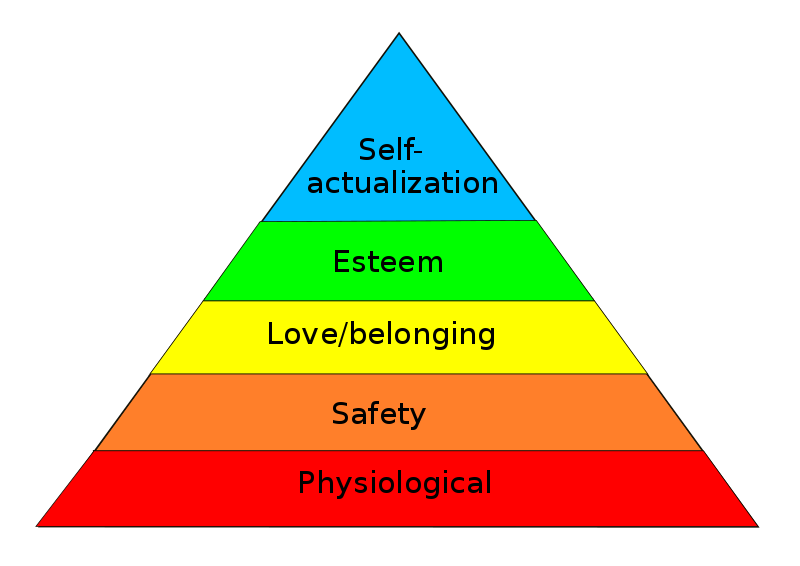
\includegraphics[width=.5\textwidth]{pictures/MaslowsHierarchyOfNeeds}
 \caption[Maslow's hierarchy of needs]{Maslow's hierarchy of needs, represented as a pyramid with the more basic needs at the bottom. Source: FireflySixtySeven via Wikipedia. \ccbysa}
 \label{fig:maslowpyramid}
\end{figure}

For example, esteem is mostly associated with extrinsic validation such as respect and recognition. However, self-esteem can be quite internal or intrinsic. Self-actualization includes art and athletics, which also have extrinsic and intrinsic motivations. Self-transcendence becomes less ego-oriented, but also can have motivations such as the need to help other humans, or intrinsic motivations such as becoming one with nature. It is clear that the higher levels of Maslow's hierarchy are less zero-sum and less competitive: the extrinsic versus intrinsic distinction changes the nature of the relationship between the individual and the community/society, as well as one's need to adhere to the social systems required for validation.

The Dalai Lama and the contemplative tradition focuses more on intrinsic motivations. While most contemplative traditions aren't necessarily anti-social, a diminished need for external validation for happiness lets one be less concerned with the opinions of others, providing more freedom and time to become self-aware and achieve happiness through the pursuit of one's personal passion or interests. This is an approach that The Venerable Tenzin Priyadarshi and I teach in my Principles of Awareness class described in \autoref{section:awareness}.

The Dalai Lama in \emph{The Art of Happiness} discusses the difference between pleasure and happiness and argues that many people feel ``happy'' when they get more money, get a new car, or progress along an externally provided measurable path. He defines these feelings as pleasures and suggests that the happiness that he describes is more like the happiness of having a happy family. Increasing the size of the family doesn't make one more happy. The Buddhist notion of happiness is quite different from happiness as described by economists who describe it as an increase in utility --- an economic measure \cite{marshall1961principles}. Later, utility was quantified by Paul Samuelson as ``revealed preference'' \cite{samuelson1948consumption} and apparently the more utility the better. The Buddhists would feel more aligned with the adage, ``more than enough is too much'' than the notion of the utility function.

\marginpar{I would suggest the word ``flourishing'' as a way to define happiness or goodness without a need to include progress or growth. A vibrant rainforest is a great example of a flourishing system.}However, many argue that progress is essential and without extrinsic motivations and economically rational humans, we would not have progress. For example, Matt Ridley argues in \emph{The Rational Optimist} that humans have an innate tendency or desire to trade. He argues that markets enable this exchange and that this exchange allows specialization --- I can help build the Internet that you use and you can design the motor for my car and use the Internet. He says that this market-based exchange of goods, services, ideas and products allows progress, and enables ideas to ``have sex'' --- computers and telecommunications coming together to turn into the Internet \cite{ridley_rational_2010}.

While the idea is exciting and helps describe how much of innovation works, he's also describing the system that, in my view, causes income inequality, exploitation of the environment, and the deployment of technologies of convenience at the cost of health. Indeed, he doesn't question whether progress is in fact ``good.''

I would suggest the word ``flourishing'' as a way to define happiness or goodness without a need to include progress or growth. A vibrant rainforest is a great example of a flourishing system. It doesn't need to grow in total size. There is diversity, there is growth and death together. There are many systems that are interconnected and the system is highly robust. While there is some controversy about methods, there is a scientific approach to measuring ecosystem robustness \cite{mumby2014ecological}. There is evolution and ``progress'' but it is slow and more like a slow adaptive search than the geometric growth or even exponential growth of human civilization.

This notion of flourishing is described in \autoref{sec:cultureflourish} and is what I believe that we must strive for in order to achieve sustainable and long-term resilience in our systems.

In \emph{The Human Use of Human Beings}, Norbert Wiener questions our idea that progress is necessarily good.

\begin{quotation}Those who uphold the idea of progress as an ethical principle regard this unlimited and quasi-spontaneous process of change as a Good Thing, and as the basis on which they guarantee to future generations a Heaven on Earth. It is possible to believe in progress as a fact without believing in progress as an ethical principle; but in the catechism of many Americans, the one goes with the other.\end{quotation}

As I wrote in the introduction, ``eudaimonia'' and productive self-actualization described by Aristotle in ``Nicomachaen Ethics`` \cite{rowe2002nicomachean} are useful concepts that includes the notions of progress towards ethics and flourishing.

\section{Interest-Driven Learning}

As I was saying, I dropped out of college twice and was even kicked out of kindergarten for running away too many times. I was never very good at education, but I liked to learn. One of my principles (see \autoref{principles}) is ``learning over education.'' I believe that education is what other people do to you and learning is what you do for yourself.

It wasn't that my schools were particularly bad or that I wasn't provided an opportunity. My sister got straight A's and went to Harvard and Stanford and got two Ph.D.s. I just had a personality that made it difficult for me to learn in a structured way about things that I didn't find useful or interesting. I also had a difficult time studying abstractions in books. I much preferred learning through doing things and talking to people.

It was very lucky for me that I was surrounded by scientists, nature, and then online computer networks and the Internet as I was entering high school. I was able to kludge together an understanding of the world's conversations by pursuing a wide variety of interests including working in a pet shop, being a disk jockey in a nightclub, working as an associate to the producer in a Hollywood film, working in a material science lab writing software for the control system, running an events company, running a computer peripherals mail order company, being a professional scuba instructor, being a record distributor, a columnist in a newspaper, a software distributor, an apparel distributor and many other things.

While I believe that I am unusually poor at structured learning, unusually motivated by my passions and interests, and unusually interested in almost everything, I do believe that interest-driven learning is generalizable.

In 1973, Ivan Illich wrote \emph{Tools for Conviviality} and argued that there are two pivotal moments in the history of scientific and societal progress. The first was in 1913 when Western medicine improved to the point where trained doctors could increase their patients' odds past 50/50. The second was when we focused more on keeping people alive than on worrying about the quality of the patient's life or their agency. Illich writes, ``I choose the term `conviviality' to designate the opposite of industrial productivity. I intend it to mean autonomous and creative intercourse among persons, and the intercourse of persons with their environment; and this in contrast with the conditioned response of persons to the demands made upon them by others, and by a man-made environment'' \cite{Illich:1973aa}.

Illich blames professional elites and economic development for negatively impacting human flourishing in modern times by institutionalizing specialization and taking control of the tools of society away from the average citizen. He believes we must ``give people tools that guarantee their right to work with independent efficiency.''

This ties to his argument that modern education focuses on institutionalization and that, as he argues in 1971's \emph{Deschooling Society}, these institutions are reducing flourishing. He argues that the educational ``funnels'' must be reversed and that we must create ``learning webs'' using advanced technology \cite{Illich:1971aa}.

The Montessori Method \cite{montessori2013montessori} of child-centered education has been used for over 100 years \cite{montessoriintro}. While the Montessori Method is much more flexible and child-guided than traditional educational systems, it still provides a teacher who guides the child by observing and responding to the child's behavior and tendencies. Unschooling, which was coined in the 1970s by John Holt \cite{unschooling}, advocates an even more radical child-directed learning approach that focuses on freeing the child from any form of formal education, depending instead on our natural ability to learn, and a belief that we will learn what we need to learn in the course of doing what we are passionate about.

In my own experience, the only practical thing that I learned how to do in my secondary formal education was touch typing. Otherwise, everything I learned, I learned out of class, except perhaps social skills that I could easily learn through group activities rather than through by sitting in a classroom. As I consider the future of schooling for my one year old daughter, I am thinking deeply about different educational options.

Jean Piaget in the 1930s said that cognitive development in children occurs as children interact with the world around them. \cite{piaget1952origins}. Seymour Papert worked with Paiget at the University of Geneva from 1958 to 1963 \cite{SeymourP62:online} and was one of Piaget's protégés. Papert was a founding member of the MIT Media Lab and developed a theory of learning called Constructionism --- student-centered project-based learning-through-doing -- that is at the core of the Media Lab, as I described in \autoref{antidisciplinaryapproach}. Papert inspired others at the Media Lab including Mitchel Resnick who argues for cultivating creative learning through ``projects, passion, peers and play'' \cite{resnick_lifelong_2018}. Resnick developed the Scratch programming language to empower children to ``code to learn'' instead of ``learning to code.'' Neil Gershenfeld is a former Media Lab professor, the director for the Center for Bits and Atoms and the inventor of the Fab Lab (short for fabrication laboratory) and the creator of the Fab Academy, a learning network. He is trying to create a network of Fab Labs to bring learning-through-making to the rest of the world. Gershenfeld says that Fab also means fabulous --- a kind of flourishing that Illich would have approved of \cite{gershenfeld2008fab}.

I believe that creativity and passion will become even more important in the future and that jobs will become even more differentiated. I also believe that learning how to follow your personal passions, rather than depending on institutions to provide motivation, will be increasingly important as jobs change and institutions go through the current industrial transformation.

Passion can come from a variety of sources. In \emph{The Wealth of Networks}, Yochai Benkler explains that the motivations for many of the online communities to produce is not financial \cite{benkler2006wealth}. In \emph{Not Just for the Money} economist Bruno Frey argues that offering higher pay may make people less committed to their work and may reduce performance \cite{frey1997not}. The social context and our desire to collaborate is a key element in developing passions.

As I write in \autoref{intro:communityvalues} Nowak and Highfield describe the evolution of cooperation and mechanisms for cooperation. They argue that evolution is not only competition but also cooperation, and that cooperation is the master architect of complexity. In ``Spontaneous giving and calculated greed,'' researchers argue that people are intuitively cooperative and thus need to ``calculate'' to overcome their cooperative impulse and become greedy \cite{rand2012spontaneous}. In ``Cooperating with the future'' \cite{hauser2014cooperating} the argument is that a large altruistic, majority would vote to cooperate with a longer view of the future in a democratic setting.

\section{Competition and Greed}

I also have competitive and greedy feelings sometimes, but they are fundamentally overpowered by my passion for the missions of my projects and my desire to collaborate and cooperate, which is supported by the studies above.

The following is an exchange on television between Phil Donahue and economist Milton Friedman from 1979 \cite{noauthor_notable_2015}:

\begin{quote}
Phil Donahue: When you see around the globe the maldistribution of wealth, the desperate plight of millions of people in underdeveloped countries, when you see so few haves and so many have-nots, when you see the greed and the concentration of power, did you ever have a moment of doubt about capitalism and whether greed’s a good idea to run on?

\marginpar{Milton Friedman: Well, first of all, tell me, is there some society you know that doesn’t run on greed? You think Russia doesn’t run on greed? You think China doesn’t run on greed? What is greed?}Milton Friedman: Well, first of all, tell me, is there some society you know that doesn’t run on greed? You think Russia doesn’t run on greed? You think China doesn’t run on greed? What is greed? Of course none of us are greedy. It’s only the other fellow who’s greedy. The world runs on individuals pursuing their separate interests. The great achievements of civilization have not come from government bureaus. Einstein didn’t construct his theory under order from a bureaucrat. Henry Ford didn’t revolutionize the automobile industry that way. In the only cases in which the masses have escaped from the kind of grinding poverty you’re talking about, the only cases in recorded history are where they have had capitalism and largely free trade. If you want to know where the masses are worst off, it’s exactly in the kinds of societies that depart from that. So that the record of history is absolutely crystal clear that there is no alternative way, so far discovered, of improving the lot of the ordinary people that can hold a candle to the productive activities that are unleashed by a free enterprise system.

Donahue: But it seems to reward not virtue as much as ability to manipulate the system.

Friedman: And what does reward virtue? . . . I think you’re taking a lot of things for granted. Just tell me where in the world you find these angels who are going to organize society for us.
\end{quote}

I think this exchange captures the essence of the capitalist ``greed is good'' philosophy that has caused the reductionist single-minded pursuit of personal wealth that has undermined robustness, resilience, flourishing and has crowded out many of the intrinsic and more positive extrinsic motivators in our society.

There is a place for competition and there is a role for self-interest, but these elements should be part of a complex system of values and drivers, and tend to address the lower elements of Maslow's hierarchy.

And one of the problems with Maslow's hierarchy is that it assumes we are individuals first and foremost. When it comes to how we run our academic system, why do we demand academics prove themselves as individuals rather than participants in a group? The tenure process and even the doctoral process focus on the individual even though their work will almost inevitably occur within and because of a social web. Some fields, such as high energy experimental physics, have begun to be more open to large collective projects, but for the most part, academics are judged as individuals. In fact, this doctoral process required me to justify why I didn't have two single authored books and two single authored papers.

The tenure process as I have observed it at MIT has the same problem and pushes junior faculty to worry constantly about seeking external validation of their individual work.

I find that my staff, including my research staff, are fundamentally less competitive and more mission-oriented than the majority of the faculty at MIT. Yet their productivity and creativity exceeds all expectations. My impression is that they are happier as well.

I often wonder whether we can have the creativity and the drive required to make brilliant contributions to society without the competition that drives many of the significant achievements.

My experience with the leaders and the community members of Creative Commons and  Internet technical communities involved dealing with some level of ``drama'' --- competition, egos and greed --- but these people and incidents felt more like anomalies and ``problems'' than the normal behavior that Milton Friedman describes so well and is so institutionalized in traditional corporate environments and in some elements of academia.

Startups have a fair share of greed but many of the successful companies are able to also have a healthy cooperative and mission-oriented socially sensitive cultures as well. This could be a shift in the demographic as young people are more concerned about the systems and less driven by the greed of their neo-liberal economic parents. The 2016 Cone Communications Millennial Employee Engagement Study showed that 64 percent of Millennials in the US ``won’t take a job if a company doesn’t have strong corporate social responsibility (CSR) values'' \cite{conestudy}.

\section{Disobedience}

\marginpar{Martin Luther King Jr. wrote, “One has not only a legal but a moral responsibility to obey just laws. Conversely, one has a moral responsibility to disobey unjust laws'' \cite{king2012letter}.}Enjoying cooperation and flourishing does not mean that we must be obedient. For systems to evolve, they require variation, mutations and diversity. Disobedience is necessary to question the status quo in science, society, law or the arts. Timothy Leary used to tell me, ``Question authority and think for yourself.'' Martin Luther King Jr. wrote, “One has not only a legal but a moral responsibility to obey just laws. Conversely, one has a moral responsibility to disobey unjust laws'' \cite{king2012letter}.

A healthy democracy, a healthy academic institution, a healthy community must be disobedience-robust. In other words, people should be allowed and encouraged to speak up against those in power without fear of retribution, and the questioning should make the system more robust, not fragile. This requires a great deal of trust between the individuals and the institution, and a strong constitution on the part of the institution to turn disobedience into positive energy.

I believe that the celebration of socially responsible disobedience is essential. You don't win a Nobel Prize for doing as you're instructed; you win a Nobel Prize by questioning authority and overthrowing previous theories. Max Planck cynically wrote, ``A new scientific truth does not triumph by convincing its opponents and making them see the light, but rather because its opponents eventually die, and a new generation grows up that is familiar with it'' \cite{planck2014scientific} which accurately summarizes the problem with our current academic system.

\begin{figure}[t]
 \centering
 
\includegraphics[width=1\textwidth]{pictures/disobedience}
 \caption{A graphic from the award ceremony for the MIT Media Lab Disobedience Award in 2017.}
 \label{fig:disobedience}
\end{figure}

With support of entrepreneur and philanthropist Reid Hoffman, since last year, I have been awarding a \$250,000 prize for disobedience from the Media lab. (Artwork from the prize in \autoref{fig:disobedience}.) As we say on the website \cite{disobedience2018}:

\begin{quote}
This award will go to a person or group engaged in what we believe is an extraordinary example of disobedience for the benefit of society: work that impacts society in positive ways, and is consistent with a set of key principles, including nonviolence, creativity, courage, and responsibility for one’s actions. We invite nominations for work across disciplines (scientific research, civil rights, freedom of speech, human rights, and the freedom to innovate, for example). 
\end{quote}

Last year, we gave the award to Dr. Mona Hanna-Attisha and Professor Marc Edwards. ``Both are scientists who became activists, using rigorous research to investigate the concerns of citizens in Flint, Michigan to unravel a mystery that many in positions of power would have preferred to keep under wraps'' \cite{disobedience2017}.

We believe that this is a small symbolic gesture but sends a signal to our community as well as to the rest of the world that we should support and celebrate positive disobedience.

\section{Civility and Governance}

Although Illich used conviviality to mean ``autonomous and creative intercourse among persons, and the intercourse of persons with their environment,'' it traditionally means friendliness. While one can actually be disobedient in a friendly way (many of my students are), it is easy to be disobedient and disruptive in an unfriendly and uncivil way.

\marginpar{I think that the ultimate role of a leader in a open non-hierarchical system is to tend to its robustness and its resilience --- to focus on its flourishing.}Whether we are talking about trolls on mailing lists as I described in \autoref{sec:emergentdemo} or world leaders taunting the public or other world leaders, the enforcement of civility or conviviality in the more traditional sense appears to be harder in decentralized bottom-up organizations.

In \autoref{intro:design} I wrote about an experiment in the feminist movement that tried to reject the idea of leaders but ended up in an informal and less accountable form of leadership, as described by Jo Freeman in ``The Tyranny of Structurelessness'' \cite{freeman1972tyranny}. Clearly having no structure is not the answer.

One study of guilds in the online game \emph{World of Warcraft} showed that guilds developed roles that focused on managing both the well-being of the players as well as the productivity and success of these guilds \cite{williams2014structural}. For many years, I ran a rather large \emph{World of Warcraft} guild, managing the diverse group of players who were paying money to collaborate with each other; \emph{World of Warcraft} charges a monthly subscription fee. Managing this community was surprisingly similar to to my role as the director of the Media Lab where the primary motivation for participating was not for the money or a very obvious progression path.

Most free and open source projects have similar dynamics --- Wikipedia, Bitcoin, Linux, etc. There is often, but not always, a core group of people who are ultimately in charge. However, most disputes are settled at the local level and through consensus.

Consensus means that everyone reaches an agreement to move forward through discussion. I learned from being on the ICANN board for three years that consensus does not require that everyone ultimately gets what they want, but that you have enough discussion so all voices are heard and the people who object to the majority eventually are convinced or get so tired that they agree to go along. Since everyone was in the room when the decision was made, they can't complain later. At ICANN we would have hours of ``open mic'' where the community would voice objections and grievances, but because we heard them out, we could reach a consensus to move forward.

Consensus doesn't always work. When you can't reach consensus you vote. Voting is never the first choice.

The role of a leader in an open non-hierarchical system is usually to manage the process, sometimes to make tie-breaking decision and sometimes to deal quietly behind-the-scenes with problems that have privacy issues that prevent a public discussion or need a speedy response that a large community can not provide.

However, I think that the ultimate role of a leader in a open non-hierarchical system is to tend to its robustness and its resilience --- to focus on its flourishing. Often it feels like gardening --- watering the plants, sometimes pruning, sometimes moving seedlings, but mostly just making sure that all of the organisms are able to be the best versions of themselves, and creating enough connections and diversity so that the garden is able to fend off the pests and bad weather by itself.

While trolls can always cause trouble as we can see from the polarization in society today, I believe that the best method for dealing with bad culture is good culture. Attacking clostridium difficile with antibiotics doesn't work well but a fecal transplant from a healthy person worked 87 percent of the time in a recent study \cite{jiang2017randomised}. The best way to fight the pathogen is to introduce a diverse and healthy culture, not try to eliminate it. Bombing terrorists has a similar effect to the antibiotics. It kills the healthy culture and makes the negative culture stronger because it ends up with more space, resources and renewed purpose. The old adage, ``Don't feed the trolls'' has a similar point. Getting angry and and focused on the trolls will deplete you of your energy, and is often exactly what the trolls are trying to achieve, giving them more energy and maybe even attracting more.

In ``Why Civil Resistance Works,'' Maria J. Stephan and Erica Chenoweth study the strategic effectiveness of violent and nonviolent conflicts between 1900 and 2006. They show that nonviolent campaigns succeeded 53 percent of the time compared to 26 percent of violent resistance campaigns \cite{chenoweth2011civil}. While the success of a nonviolent campaign is still only a coin-toss, it's statistically more likely to succeed in the conflicts that they studied than violent resistance. The notion of ``satyagraha'' or ``truth force,'' espoused by Gandhi \cite{majmudar2012gandhi} is, in my view, the most effective form of non-violent action.

While most non-violent action is typically employed by communities fighting against the establishment, the basic tenets can work in undermining and disabling negative individuals or sub-communities. In the long run ``taking the higher road'' is the most sustainable way to build a a trusting and robust community with a strong positive culture.

\section{Self-Awareness and Humility} 

Whether we are talking about trolls or participant design, the key is to focus on doing a better job yourself instead of trying to tell others what to do or how to do it. I believe that whether we are talking about an individual or an institution, striving for strong core values and excellence, and being open, transparent, and accessible allows others to copy the patterns that work for them in their context. It's important to design organizations for transparency because it's difficult to transform closed organizations into transparent ones \cite{Ito2011Designings}.

Communities are defined by their differences: differences in diversity, size, resources, mission, history, and technical landscapes. Good values can transfer across communities, and adjacent communities can adopt sensibilities and ideas, translating them into local values. We have seen that courage --- from Gandhi's image on the cover of \emph{Life Magazine}, to the Tunisian protesters on social media, to the Parkland students --- can transmit across communities very quickly.

I believe that the most humble, and the most effective, approach to changing the world is to make yourself and your own community better and more flourishing, and to share ideas and connections as freely as possible.

For this, communities and individuals need to become self-aware and reflective so that they --- we --- are able to deprogram the conditioning of decades of institutional education, institutionalized social inequity, and ``greed is good'' justifications for exploitative capitalism. Only thus can we continue to strive to make ourselves better versions of ourselves. 

(How ``better'' is defined will be covered in future work.)
 % Chapter 5 - culture of change - NEW CHAPTER!

%\cleardoublepage
%\ctparttext{\textbf{Part III} is a conclusion which reflects on the learnings from successes and failures in applying the theory of change on the areas described in Requiring Change. From these learnings, I discuss and explore how the work can continue and possibly be applied by others.} 
%\part{Conclusion} % Third part of the thesis

\chapter{Conclusion}
\label{chap:conclusion}
The modern problems such as climate change, health, and societal inequities are complex and adaptive, and the only way to address them is through a paradigm shift away from reductionist market-based economic growth to a more sustainable and complex paradigm focused on flourishing. I have shown through examples that while computers and the Internet have added to complexity and speed, they also provide a way to redesign ecosystems and communities.

I explored the history of disciplines and used the example of the Media Lab to illustrate how the problem of silos created by disciplines may be addressed with an antidisciplinary approach, providing new academic communities with different values, funding, and reward structures. I have shown how this antidisciplinary approach can be applied effectively to tackle complex problems in many domains.

To tackle the world's wicked problems, I suggest a combination of the antidisciplinary approach and intervention in complex systems through a humble form of participant design and the transformation of values through social and cultural movements, using my days as a DJ, and my immersion in hippie and early Internet culture as an example.

I presented my ongoing work on transforming democracy and the public sphere and several new initiatives in space exploration, health care, and the governance and ethics of artificial intelligence as fields where I am testing my theory of change.

\section{Contributions}

This dissertation has addressed five central challenges: 

\begin{enumerate}
\item Draw on the history and philosophy of science and the learnings from operating the Media Lab to describe and explore the antidisciplinary approach and how it can be implemented effectively in an institution and a community.
\item Develop ideas from cybernetics, systems dynamics, evolutionary biology, and design as a way of understanding and intervening in complex adaptive systems through a method of cultural interventions in communities.
\item Show through examples how the values of decentralization and unbundling layers that emerged as the architecture for computing and the Internet can be applied to other domains such as finance, medicine, and climate.
\item Define the role of cultural movements in paradigm shifts and propose this as a way forward with the trifecta of wicked problems --- climate, health, and social inequality.
\item Define the importance of governance and ethics in the future of machine learning and artificial intelligence, and show how antidisciplinary scholarship and activity can advance the integration and appropriate deployment of machine learning and artificial intelligence in society.
\end{enumerate}

\section{The Learnings}

Throughout my practice, beginning with my experience working as a DJ in a nightclub and through my work on many layers of the Internet through for-profit and non-profit work, and cumulating in my current work at the Media Lab, there are consistent learnings.

\begin{enumerate}
\item The Internet has fundamentally changed the ability of communities to form and manage themselves at low cost while massively increasing the complexity of the environment.
\item Communities flourish with strong values that provide a shared mission beyond a purely financial one.
\item If the mission has a strong commons-based societally beneficial focus, the community can increase the resilience and flourishing of the broader ecosystem of communities.
\item Communities built around science, technology and innovation can be highly generative and creative with the right values and architecture.
\item The technical, legal, normative and financial architecture must be designed to provide a structure within which such communities can thrive, and for a community to appropriately interact with other communities in the broader ecosystem.
\item Leadership and design interventions in high functioning communities are participant-based, humble and have distinct differences from traditional top-down industrial firms.
\item An antidisciplinary approach can allow communities to transcend existing paradigms, and the Internet provides an opportunity to re-architect higher education and the development of knowledge and disciplines to support such an approach.
\item Complex scientific and social endeavors, such as designing Geiger counters and deploying them through workshops and kits, can be accomplished through a networked, mostly volunteer organization. 
\item Visionary leaders generate revolutionary new organizations and structures, but a more community-based leadership/management model is required to transform these organizations into sustainable and flourishing communities.
\end{enumerate}

\section{Future Work}

\begin{enumerate}
\item While the Media Lab has successfully developed an antidisciplinary approach to develop new disciplines and connect to existing ones, its rejection of structure has led to problems of structurelessness. Mentoring faculty in a system where each faculty member is unique and mentoring students in a structureless system is challenging. While the idea of learning through doing and collaborating to produce cross-disciplinary rigor does work, it is not a scalable system of knowledge. The consortium model of funding we use at the Media Lab has limited the negative effects of narrow funding sources, and our focus on research through making decreases the narrowing of peer-review for our own academic program. But we have yet to come up with new structures for knowledge, and can improve on the community's ability to manage the rigor and the quality of the work. The current Media Lab culture is generative and successful, but as we engage in harder sciences and try to interact with a broader community, additional structure and clarity may increase our effectiveness.
\item Mindfulness and the adoption of healthier and more personal motivators are key for the transformation of our values, but contemplative practice does not scale without losing many of its core attributes. Work on interventions that expand opportunities and incentives for contemplation, as well as ways to allow individuals to become more self-aware, can be developed.
\item The constructionist approach of the Media Lab helps theory through practice and practice through theory, but deploying that approach in the real world of criminal justice systems, health care systems, climate change advocacy, and other functioning systems goes beyond the scope of academic research. Creating nonprofit and for-profit spin-outs from the Lab, participating personally in non-academic operating entities disconnected with research at the Lab to avoid a conflict of interest issues, and formally partnering with operating entities through the technology licensing process have been the primary methods of deploying and expanding our practice and theory. Institutional development at MIT and similar institutions must be undertaken so that they can more actively engage for-profit and nonprofit startups to bring deployment closer to research.
\item Cryptocurrency and blockchain technology have many similarities and some key differences from the development of the layers of the Internet. But the for-profit focus and exuberance of that community is hampering the development of the non-profit and academic consensus and the protocol layer that is so essential to the Internet model. We must continue to apply what we have learned from the Internet to the evolution of blockchain technology.
\item While Creative Commons and the Open Source Initiative have contributed towards interoperability and reducing friction at the copyright layers, we still have many problems including a patent system that is stifling innovation by favoring large companies and by enabling frivolous patent filings and lawsuits. We are also challenged with the relationship between privacy, copyright and the use and abuse of data for both good and harm. While there are interesting conversations and new regulations, there is a great deal of technical and regulatory work required to solve intellectual property and data sharing on the Internet.
\end{enumerate}

\section{Call to Action}
\begin{enumerate}
\item With a combination of experiments to examine the human body; the development of new tools to interact with the human body, and the antidisciplinary application of knowledge from a variety of fields, we must re-imagine and redesign our understanding of, and ability to, intervene in our health system. This will require the creation of new research institutions and communities as well as the deployment of new business models.
\item We must advance beyond the ability to organize collective action through movements powered by the Internet and understand and deploy ways to scale the development of institutions, trust and collaboration --- a new democracy for the post-Internet era.
\item We must tackle the vital problem of climate change by creating a social movement with the tools we have developed for the Internet, drawing on learnings from historic arts and cultural movements.
\item We must shift from centralized, control-oriented design and engineering to participant design in all fields of endeavor and study, including space exploration, redesigning the financial system, and integrating machine learning and AI into society in fair and appropriate ways.
\item We must redesign academic publishing so that it becomes a viable platform and framework for sharing knowledge open and globally in the post-Internet, highly complex and antidisciplinary world.
\item We must develop and tweak the Safecast model of networked citizen engagement so that it can be used in other domains.
\end{enumerate}

\section{Summary of Chapters}

\emph{Chapter One: Introduction.} I present my introduction and an overview of the dissertation.

\emph{Chapter Two: Requiring Change.} I first explore the history of science and the creation of knowledge and disciplines. There is an historical view that disciplines are social and community-oriented, structured around power and community architecture more than ``truth.'' I describe the idea of antidisciplinary work between and beyond the disciplines and note that it is particularly important as the world has become more complex and faster thanks to the Internet. I suggest that we need to shift our paradigms away from control-oriented interventions to participant design as the problems become too complex to control. I propose that influencing the values of a community might be a better way of causing paradigm shifts. I share my fear of the singularity movement as the next big reductionist movement and urge us to resist reduction. I present the hippie movement and its influence on the Internet as an example of a relationship between a cultural movement and a generative technical community.

I then outline five areas that I believe we can change. I describe the issue of silos that emerge from academic disciplines and how an antidisciplinary approach might be more effective. I describe how monolithic and centralized systems are being successfully unbundled; how the Internet was the first major success of unbundling, and how banking is now beginning to be unbundable thanks to blockchain technology. I describe the post-Internet public sphere and how social media has emerged in the context of the history of blogging. I then express my concern that we have used the Internet to dismantle institutions without using it to rebuild them robustly, thus undermining our faith in them. I worry that we have so far done more damage to the public sphere than we have done to help it, and that a similar situation could emerge for the future of health care: the pharmaceutical industry could fail before we have a viable alternative. I describe the pharmaceutical industry's struggle to keep up with the changing landscape of complexity and tremendous amounts of new data and tools. Climate is a similarly complex and potentially more disastrous problem that requires a fundamental change in the way we think as well as the way we intervene in it. We need social movements and participant design. It is all about community.

\emph{Chapter Three: Theory of Change.} I describe different types of people --- specialists, interdisciplinary people, multidisciplinary and antidisciplinary people --- and suggest that the role of the Media Lab and antidisciplinary people is to connect different disciplines and explore the spaces between and beyond them. I suggest that we might develop more structure, new values, and a new practice beyond just being antidisciplinary to create a new method for the development of knowledge.

I propose the idea that building of layers into the Internet's architecture, with commercial layers sandwiched between not-for-profit commons-oriented protocol layers, was the key to its success.

I give examples of the Digital Millennium Copyright Act, wiretapping laws, and anti-money laundering laws as laws that no longer work well and consider how we might use an antidisciplinary approach and Lessig's notion of the synthesis of law, markets, norms and technology in navigating these issues.

I share an essay on the nature of the Internet as a medium with aesthetics that influence its nature, art, and sensibilities.

I propose that activating communities is the key to paradigm shifts and share my experience as a DJ in a nightclub and the role that music had on various communities as an example of the role played by culture and sensibilities. I also use my experiences in nightclubs as a lens to see how the dynamics and reality of communities are nearly impossible to understand from the outside, and how working-class and bottom up values are important and underestimated by elites. I discuss the hippie movement and its methods and reflect on how we might consider the design of, and participation in, movements in the post-Internet era.

\emph{Chapter Four: The Practice of Change.} I draw on my experience and practice to illustrate the application of the theory of change.

The Internet and layers of the Internet with protocols such as \ac{TCP/IP} and \ac{HTML} have become wildly successful. The open source and free culture ecosystem has thrived in part because of the success of Creative Commons licenses and open source licenses verified and managed by the Open Source Initiative. Participating in the not-for-profit organizations that stewarded the protocols and the governance --- \ac{ICANN}, The Open Source Initiative (OSI), The Mozilla Foundation, Creative Commons, Computer Scientists for Social Responsibility (CPSR) and The Electronic Privacy Information Center (EPIC) --- helped me contribute to the success of the Internet's not-for-profit protocol layers as well as gaining an understanding of the ecosystem.

Helping build the first commercial Internet Service Provider in Japan, Infoseek, one of the first algorithmic search engines in Japan, helping launch the first banner ad network sold by impressions, helping to starting the first blogging software company in Japan, and helping to start the first and now largest payment settlements company in Japan provided an opportunity for me to contribute to, and learn from, the execution and scaling of the Internet and its services commercially.

Participating in numerous government committees helped guide regulation of the Internet, including laying the groundwork for independent ISPs in Japan, participating in writing the first hacker bill in Japan, and protesting, unsuccessfully, the national ID in Japan.

These activities substantially contributed to the development of the Internet ecosystem in Japan and the world. I learned a great deal about multi-stakeholder organizations such as \ac{ICANN} and Creative Commons and how the communities can be managed to provide technical, normative and coordinating outputs. In addition to mission and leadership, such communities require rules, business models, and internal and external communication structures, which I describe in the implementation section.

Through publishing, blogging, and participating as a board member of \textit{The New York Times} and the Knight Foundation, I have explored and helped lead a conversation about the future of media and the public sphere. Our initial ideas were clearly optimistic about the nature of the transformation but accurate about the degree of impact. My efforts continue through work on the governance and ethics of artificial intelligence, through scholarship, deploying interventions, and teaching in order to improve the public sphere and the democratic governments that it serves.

Learnings from the Internet inform my management of the Media Lab which is also a generative, mission-driven community engaged in permission-less innovation. The Media Lab tackles the problem of siloing created by the disciplines through an antidisciplinary approach to scholarship and research. Together with the MIT Press, the Media Lab is tackling the future of antidisciplinary scholarship through reinventing academic journals and publishing.

Digital currencies and blockchain will potentially be another layer on the Internet stack and promise to be as transformative of law and finance as the Internet was to the media and commerce. I have described my work in advancing the field from the early days in the 1990s and 2000s testing early implementations such as Digicash, to supporting the early work on digital signatures and participating in an ambitious and failed attempt to build a data center, Havenco, beyond the reach of governments. I describe the creation of a substantial non-profit research effort in the form of the Digital Currency Initiative at MIT which hopes to help manage the protocol and community management required for digital currencies to flourish.

This antidisciplinary approach is being applied to understanding and designing interventions in the wicked problems of climate change, health and income disparity. Creating new sensibilities, communities, organizations, structures, scholarship and a new sensibility to improve our regulation and ability to flourish is essential. There is still a great deal to be done and each of these domains will necessarily be very different from each other, but many of the learnings and systems that I have helped create will contribute to our ability to improve our outcomes.

\emph{In Chapter Five: The Actors of Change.} I define happiness and differentiate between ``pleasure'', simple reward systems, and happiness through a sense of flourishing. I explore the history of interest-driven and constructionist learning for myself and the Media Lab. I discuss the role of cooperation and greed. I argue for the importance of disobedience in advancing science, law and institutions and the importance of disobedience robustness in organizations. I suggest ways that we might manage organizations to deal with not-so-beneficial troublemakers and trolls, and thoughts on the importance of self-awareness and humility in leaders.

\section{Looking Ahead}

The birth of the Internet and related technologies gave us hope that a new architecture would give us new values and a way to scale society up and out of many of the problems that faced us. It felt quite optimistic as many of our architectures and technologies revolutionized the way we did things.

As we face the reemergence of monopolies, polarization, and greedy feeding off of the commons on earth and possibly in space, many of us wonder if these social issues of humanity are pendulum-like, swinging from left to right, open to closed, optimistic to pessimistic over time --- or if they generally get worse with bumps along the way, or is true, as Martin Luther King said, paraphrasing the Unitarian minister and prominent abolitionist Theodore Parker, that ``The arc of the moral universe is long, but it bends toward justice \cite{parker1853justice}.''

That, I believe is for us to see and for us to cause.

\section{What's Next}

\subsection{The Internet}

We see that over and over again, the communities that grow up around new technologies and networks, mailing lists, Usenet, open source projects, email, and independent ISPs have difficulty retaining their core momentum and eventually break up through some combination of pressure from the outside; a flood of ``newbies'' dilutes and diverts the culture, or a layer of technology becomes irrelevant.

The ideas of openness, freedom, sharing and civility that we hoped to ``lock in'' when we designed the Internet were clearly subverted.

In addition, architectural elements such as the unbundled layers of interoperability and competition that the early ISPs exemplified have disappeared. Telephone companies and cable companies in the United States acquired or otherwise eliminated independent ISPs. Some countries still have them, but they are rare and not nearly the broad communities that they once were.

At the same time, the Internet has gone mobile, but there was no opportunity to unbundle the mobile system. As a result, we have a mostly metered and monopolized mobile Internet that costs far more than necessary, inhibiting basic activities such as roaming.

While activist organizations such as the Electronic Frontier Foundation and the American Civil Liberties Union continue to fight for the core principles of freedom on the Internet, it appears that the movement to keep the Internet open and free is diminished in power.

Even Apple, which initially provided us with the blinking cursor and a computer asking to be programmed, now makes it difficult and even scary to execute anything but officially approved applications. And ``jailbreaking'' your phone will break your warranty, if not land you in jail.

The world has gotten scarier and more dangerous and so it does make some sense that services are less open and generative, but the telecom and technology companies are clearly using this as an opportunity to lock in their control.

Although the recent issues with Cambridge Analytica and Facebook cannot be called ``bright,'' they have brought privacy to the fore of many citizen's concerns. The General Data Protection Regulation (GDPR) in Europe is bringing these issues into regulation. Ironically, it may turn out to be government that takes the lead into the next phase of Internet civilization.

\subsection{Blockchain}

At the Media Lab, we have convened a group of strong researchers and academics from diverse and relevant backgrounds to work on the issues raised by blockchain technology. The core members of our group do not have financial interests in cryptocurrencies and are not biased financially. We are clearly playing an important role by making public comments, advising governments, and thinking long term about the development of the blockchain for social good.

While I theorize that the blockchain will go through a development pattern similar to that of the Internet, with layers, interoperability, non-profit non-governmental coordinating bodies, and layers of venture businesses in between, there are some clear differences.

We do not have identifiable community leaders like Jun Murai, John Postel, Richard Clark, Vint Cerf, Steve Crocker, Tim Berners-Lee and others who can take the lead in bringing communities around blockchain together. Cryptocurrencies originally had an anti-government culture that it is now growing out of but still has its roots in, whereas the Internet was quite government-friendly for the most part. The blockchain is stateful and technically quite different from a communications layer. Lastly, but perhaps most importantly, the financial impact of the blockchain has eliminated at least a decade of time, if not more, for the technical and hobby people to play with standards and technologies before trying to build businesses on top of it.

I still believe that Bitcoin has the most substantial community, but it is missing some coordinating ability, a compelling culture and leadership.

Regardless of these caveats, I believe that it is critical to try to develop a community around Bitcoin and support its development using all of the tools and the methods so far discussed.

\subsection{The Commons}

Creative Commons licenses have continued to grow, and they are now an important part of the publishing ecosystem. We have not, however, solved the problems of open access to knowledge and academic publishing.

Free and open source software have become a standard and valuable part of the ecosystem, but their use and management can still be improved. In fact, the fact that Bitcoin is an open source project is a significant contributor to its success, and in the field of cryptography where peer review is essential, it is nearly impossible to have a non-open source project.

Patents are still a major problem for small companies that compete with large companies. Individual researchers are also victim in many cases to large company patents. The patent system clearly needs an overhaul.

Both the open source community and Creative Commons have tried to address the problem, but we may require government, academia and businesses to work together to resolve this.

\subsection{Health}

We are just embarking on the implementation of what we have learned about communities, breaking up the silos, and creating new disciplines, and the response from researchers, regulators and businesses has been exciting. The initial workshops and meetings have been productive, and the active participation of the U.S. Food and Drug Administration is heartening.

The complexity of the problem and the number of pieces that we must manage is daunting. I am also concerned that, as with media and the Internet, it is possible that we destroy the old model before we have come up with a new one.

One impediment is the difficulty of integrating commercial ventures and academic scholarship because of conflict of interest policies put in place to protect the neutrality of academic research. Designing better ways to translate research from academic research labs into commercial deployment has a great deal of opportunity to improve.

\subsection{Space}

The Space Exploration Initiative, like the Health 0.0 project, is also an emerging project that addresses a very diverse community, tying in to existing efforts at MIT in the Department of Earth and Planetary Sciences and the Department of Aeronautics and Astronautics. The event this year for the initiative was the most watched event in the history of the Media Lab online.

Danielle Wood, a new faculty member of the Media Lab, pointed out during the event that we should avoid the term ``colonizing space'' since the word ``colonizing'' has its roots in extractive, exploitative conduct by the West. We should be more reflective and respectful of space. The issue of whether we have the right to treat space as something we can own and what our relationship to space should be has many parallels with the way we have treated earth. We are already beginning to understand the damage we have caused by strewing space junk in our orbital space around the earth.

The issue of the law of space has many similarities to the ``laws of cyberspace,'' where we try to understand how to manage ourselves in this extra-jurisdictional space and protect the commons.

The diminishing cost of participating in space exploration has some parallels to the effect that the Internet has had on many fields. The the initiative and the diversity and number of projects proposed for it show how similar it is to the development of the Internet. The application of Internet learnings on space will be an interesting area of exploration.

\subsection{The Environment}

\subsubsection{Nia Tero}

Nia Tero strives to protect the climate through the protection of indigenous people. At a recent meeting, we discussed the notion of ``natural capital.'' This is the idea that if we account for the carbon, the trees, and the fish, and track the ``assets'' that companies and society are extracting from the environment, it would help us account for these externalized costs and manage companies and natural resources better. One of the indigenous leaders pointed out that to him, the term ``natural capital'' sounded like an oxymoron. Nature does not belong to us. We belong to nature. The idea that nature should be in our accounting systems might make sense if we are trying to tackle the climate and environmental issues using the market and ``enlightened best interest'' to solve the climate problem, but the true paradigm shift would be to adopt the sensibility of indigenous people and make it feel ``wrong'' to everyone to just take from nature.

At a recent meeting in Hawaii on Earth Day 2018, I was involved in a discussion about the Rodium Group's ``Transcending Oil: Hawaii’s Path to a Clean Energy Economy'' report \cite{Transcen68}. The report shows that Hawaii can be completely free from fossil fuels by converting to renewable energy. The report lays out a clear argument that the economics work. As we discussed the issues, it became clear to me that what we were talking about was the transformation of existing institutions and the transcendence of existing paradigms developed around a notion of centralized control of a fossil fuel-based energy resource and supply chain. The decentralized and ``out-of-control'' idea of a power grid that connected everyone with solar energy generators was a completely different paradigm, but that paradigm, at this point, is a greater challenge than the technology.

Interestingly, the behavior of energy utilities is extremely similar to the behavior of telephone monopolies during the development of the Internet, and it appears that the challenges and benefits of decentralization and unbundling will be very similar.

\subsubsection{Safecast}

We learned from the Safecast experiment that we can mobilize engaged scientists and citizen activists by engaging them in a movement. The Safecast movement involved social activism and active participation in the building, deployment, use and sharing of the system. The open data platform was key. Safecast has emerged as an extremely successful model, and we are being pulled into new areas of bottom-up participatory science in adjacent spaces such as air quality.

\subsection{Media Lab}

As the Media Lab enters its fourth decade and begins working in the hard sciences and grappling with the complex problems of health, climate and social inequity, we must reposition it among the disciplines. The Lab also has become less constrained financially, and we must now consider the limits of growth and the way in which we select our domains and define limits.

More work in the hard sciences also increases the necessity for a more structured system of knowledge development beyond the antidisciplinary.

\section{Concluding the Conclusion}

The future of humanity depends on our ability to understand and intervene in society in order to minimize the impact of climate change: halt and reverse damage from social inequity; stop the march of chronic disease, and consider new ways of thinking about health; maximize the benefits of new technologies while minimizing their detriments; and explore new areas such as space and the blockchain.

We can apply the ways we unbundled power and created layers to organize and build the Internet to many cases that analogs, even if they don't work exactly as the Internet does. 

Understanding the systems and levers of intervention using Lessig's laws, markets, technical architecture, and norms is key. (See \autoref{fig:lessigian} for diagram of Lessig's quadrants.) An antidisciplinary approach and community are key. Donella Meadow's notion of intervening at the paradigm level is key \cite{meadows_leverage}.

The creation of this capacity, as well as the ability to manage the change that it will produce, requires a healthy and well-designed community and movement. The Media Lab can experiment with community design and management itself, as well as new initiatives being developed at the Lab. Hopefully the Media Lab and the projects and the people who pass through it will serve as inspirations to others to use, adapt, transform, and share our ideas and methods.

Supporting the Media Lab in these efforts will be the focus of my work for the foreseeable future.
 % Chapter 6 - conclusion

\cleardoublepage % Empty page before the start of the next part

%----------------------------------------------------------------------------------------
%	THESIS CONTENT - APPENDICES
%----------------------------------------------------------------------------------------

\appendix

%\part{Appendix} % New part of the thesis for the appendix

% Appendix A

\chapter{Professor of the Practice Research Statement}
\label{ch:researchstatement}


\emph{Following is the research statement that I presented to the Massachusetts Institute of Technology for my promotion case to Professor of the Practice in Media Arts and Science in March of 2016. The statement describes my vision for the Media Lab and my role. The case was successful.} \\

\textbf{Research Statement} \\

Science, engineering, design, and art can together be viewed as a circle where the output of one is the input of another. Design and science are opposite each other on this circle; that is, the output of one is not the input of the other, as is often the case with engineering and design, or science and engineering. I believe that by making a ``lens'' that fuses design and science, we can fundamentally advance both. 

When I joined the Media Lab in 2011 as its director, ``antidisciplinary'' was a word new to me. It was listed as a requirement in the faculty search description. Antidisciplinary, as opposed to ``interdisciplinary,'' is about working in spaces outside the traditional academic disciplines --- about a new way of working without the traditional tools, such as a focus on a particular scale and a specialized language, that typify the current scholarly research. By bringing design and science together, we can foster new, productive, and flexible antidisciplinary work. 

In many ways, the cybernetics movement of the 1940s and 1950s has served as a model for what the Media Lab does --- drawing on new technologies to create a movement cutting across disciplines. Cybernetics spawned many exciting new disciplines but, as a field, it fragmented, with the offspring of the intellectual leadership ending up in many of these newly established fields. My aim is to develop a movement that is agile, engaging, and antidisciplinary enough not only to survive but to thrive on its own even as new disciplines spin off.

We are looking for people who don't fit into any existing field of study. I often say that if you can do what you want to do in any other lab or department, you should go do it there; come to the Media Lab only if there is nowhere else for you to go. We are the new \textit{Salon des Refusés}.

Another analogy for the space I'm promoting: Think of a sheet of paper representing the whole of science. Its various fields are black circles on this paper. The white space between circles represents antidisciplinary space. Many people would like to play in it, but there is very little funding for them; moreover, it's often hard to get a tenured position without some sort of anchor in one of the disciplinary circles. 

The Internet and increasingly more powerful computational tools, accelerated the rate at which research can be conducted, shared and combined. This has generated a new opportunity but also increases the complexity, making it increasingly difficult to tackle many of the interesting problems through a traditional disciplinary approach. Unraveling the complexities of the human body is a perfect example. Brain research, for instance, involves a diversity of disciplines, among them computational optics, nanotechnology, data science, systems biology, and the microbiome. Therapeutics are just as diverse, encompassing pharmacology, electromagnetic interactions, and opto-genetics as well as nanotechnology. Traditional interdisciplinary research involved bringing researchers together across these disciplines, whereas increasingly, the key researchers are able to straddle multiple disciplines and translating and synthesizing in a way that is difficult or impossible as a conversation between disciplines. Many current efforts seem unable to move beyond a mosaic of so many disciplines that often we don't realize we're all looking at the same problem, so different are our methods, our instruments, and our language. 
While the space between and beyond the disciplines can be academically risky territory, it allows for promising unorthodox (and often cheaper) approaches that draw on hitherto insular regimes. The Internet's enabling of collaboration at nearly no cost, as well as the diminishing costs of computing, prototyping, and manufacturing, also contribute to the flexibility of antidisciplinary research. \\ 

\textbf{Addressing the World Through This New Lens} \\

Whereas science arguably moves toward this antidisciplinary convergence, design has become what Marvin Minsky, in The Emotion Machine, calls a ``suitcase word'': It means so many different things that it means effectively nothing. Design, as I use it here, refers to the iterative process of understanding the constraints of a system and creating something that will have an effect on it. Unlike engineering, design is not as much about solving problems as asking questions. The designer is the architect, the maker, the scientist who introduces a new point of view. It encompasses many important ideas and practices, and thinking about the future of science in the context of design promises to be a fruitful endeavor.

Design has progressed from the design of objects to the design of systems and on to the design of complex adaptive systems. This evolution is shifting the role of designers, who should be seen not as planners apart from, but as participants within, the systems they exist in. Today they work for companies or governments, developing products and systems focused primarily on ensuring that one or another aspect of our society works efficiently, with scant concern for systems beyond specific corporate or governmental needs. But we're moving into an era in which system boundaries are not as defined. These underrepresented systems—the microbial world, say, or the global climate, or the environment—present significant design challenges. They are self-adaptive complex systems, and our unintended and unexamined effects on them will most likely have negative consequences for us.

Media Lab professor Neri Oxman and architecture professor Meejin Yoon co-teach a popular class called ``Design Across Scales,'' in which they discuss design at scales ranging from the microbial to the astrophysical. While it is impossible to predict the outcome of complex self-adaptive systems, we can indeed hope to understand and take responsibility for our interventions within them. This is designing absent the ability to control-—more like giving birth to a child and influencing its development than designing a robot or a car.

An example of this kind of design is the work of Media Lab professor Kevin Esvelt, who describes himself as an evolutionary sculptor. He is working on ways of editing the genes of populations of organisms such as the rodent that carries Lyme disease and the mosquito that carries malaria, to make them resistant to those pathogens. His aim is to effect a change in the genome that will spread throughout the entire population of the organism. Thus its consequences will alter the whole ecosystem, including the biosphere, public health policy, and the ethical issues attendant on these sorts of interventions. What is novel here is consideration of the effects of a design on all of the systems that touch it.

When the cybernetics movement began, the focus of science and engineering was on such tasks as guiding a ballistic missile or controlling the temperature in an office --- problems squarely in the man-made domain and simple enough to yield to traditional siloed methods of scientific inquiry. For those of us working in the contemporary space of design and science, there are no obvious boundaries in the territory we are addressing. Formerly there was a clear separation between the artificial and the organic, the cultural and the natural. Today, the man-made and the natural are no longer separate --- they are one. 
Science and engineering now pursue problems in synthetic biology and artificial intelligence --- undertakings so complex they extend beyond the domains of existing disciplines. We are finding that in many ways we can now ``design'' nature. Artificial intelligence, for example --- a digital rather than a natural science --- is moving beyond a merely metaphorical relationship to the human brain. By picking up where cybernetics left off and redirecting the development of modern design to the future of science, we believe that a new kind of design and a new kind of science may emerge, and in fact is already emerging. \\

\textbf{Rethinking Traditional Academic Research} \\

I envision a new model for academic research and collaboration that breaks down the barriers dividing the disciplines. Building on the foundations of the Media Lab, I will create a vehicle for the exchange of ideas --- a vehicle that brings those working in antidisciplinary space together in exciting ways that challenge existing academic silos. My ultimate aim is to create a new platform and network for the 21st century: a new way of thinking and doing that will spread beyond the Media Lab, and beyond MIT.

Much of academia revolves around publishing research in prestigious, peer-reviewed journals. The peer review of academic papers was important in building scientific knowledge before the Internet, but in many ways it is holding us back now. It often leads researchers to focus on proving the value of their research to a small number of experts in their own field rather than risking an unconventional approach --- thus reinforcing a cliché of academia: ``learning more and more about less and less.'' And it exacerbates a hyperspecialization whereby people in different fields have trouble collaborating, even communicating, with one another. The Media Lab has just launched a new antidisciplinary journal with MIT Press, called The Journal of Design and Science, which is built on an open-access, open-review, rapid publication platform called PubPub, created by Media Lab students Travis Rich and Thariq Shihipar. As the curator of the new journal, I will work on creating a model of interaction online; many of the contributions will be snapshots of in-person conversations. This intimate form of communicating is in stark contrast to the formal peer-review system, allowing contributors to tackle the most interesting problems and ideas of our times; it is itself an experiment.

In addition to building this new way of collaboration and publishing, I would like to develop a new, hybrid research-and-development process --- a translation process that will deploy academic research into the real world and bring the real world into academic research. I intend to establish a program based on the original Media Lab design but serving as a link between MIT and the outside world. As participants/designers, we will be focusing on changing the way we do things in order to change the way the world does things. Thus I will recruit collaborators from across MIT and beyond. I have already launched a number of initiatives that are examples of this innovative outreach: 	

\begin{enumerate}
\item ``Extended Intelligence'' is the study of machine learning and AI as a human/machine system --- a fundamentally distributed phenomenon --- across scales from the neuronal/electrical, to interface design, to networks, to the formation of relevant policy and ethical standards for human/machine interaction.
	
\item The Media Lab Digital Currency Initiative enlists experts in computer science, cryptography, economics, and fiscal policy to work with a community of developers, companies, and government and public institutions on exploring the many issues involved in blockchain and bitcoin technology.
\end{enumerate}
	
The Age of Enlightenment centered on structured reason and heralded a new age of science. We are entering another new age --- one in which structured reason is not enough. A new kind of science is emerging, based on designing novel methods of addressing complex adaptive systems --- systems that remain beyond our ability to fully understand. My work will contribute to a new way of conducting antidisciplinary but rigorous research with global effects that will allow us to survive and flourish in this new age we have entered.

% Appendix B

\chapter{Letter 1 to Massachusetts Legislature On Pretrial Risk Assessments}
\label{appendix:A}

\newpage

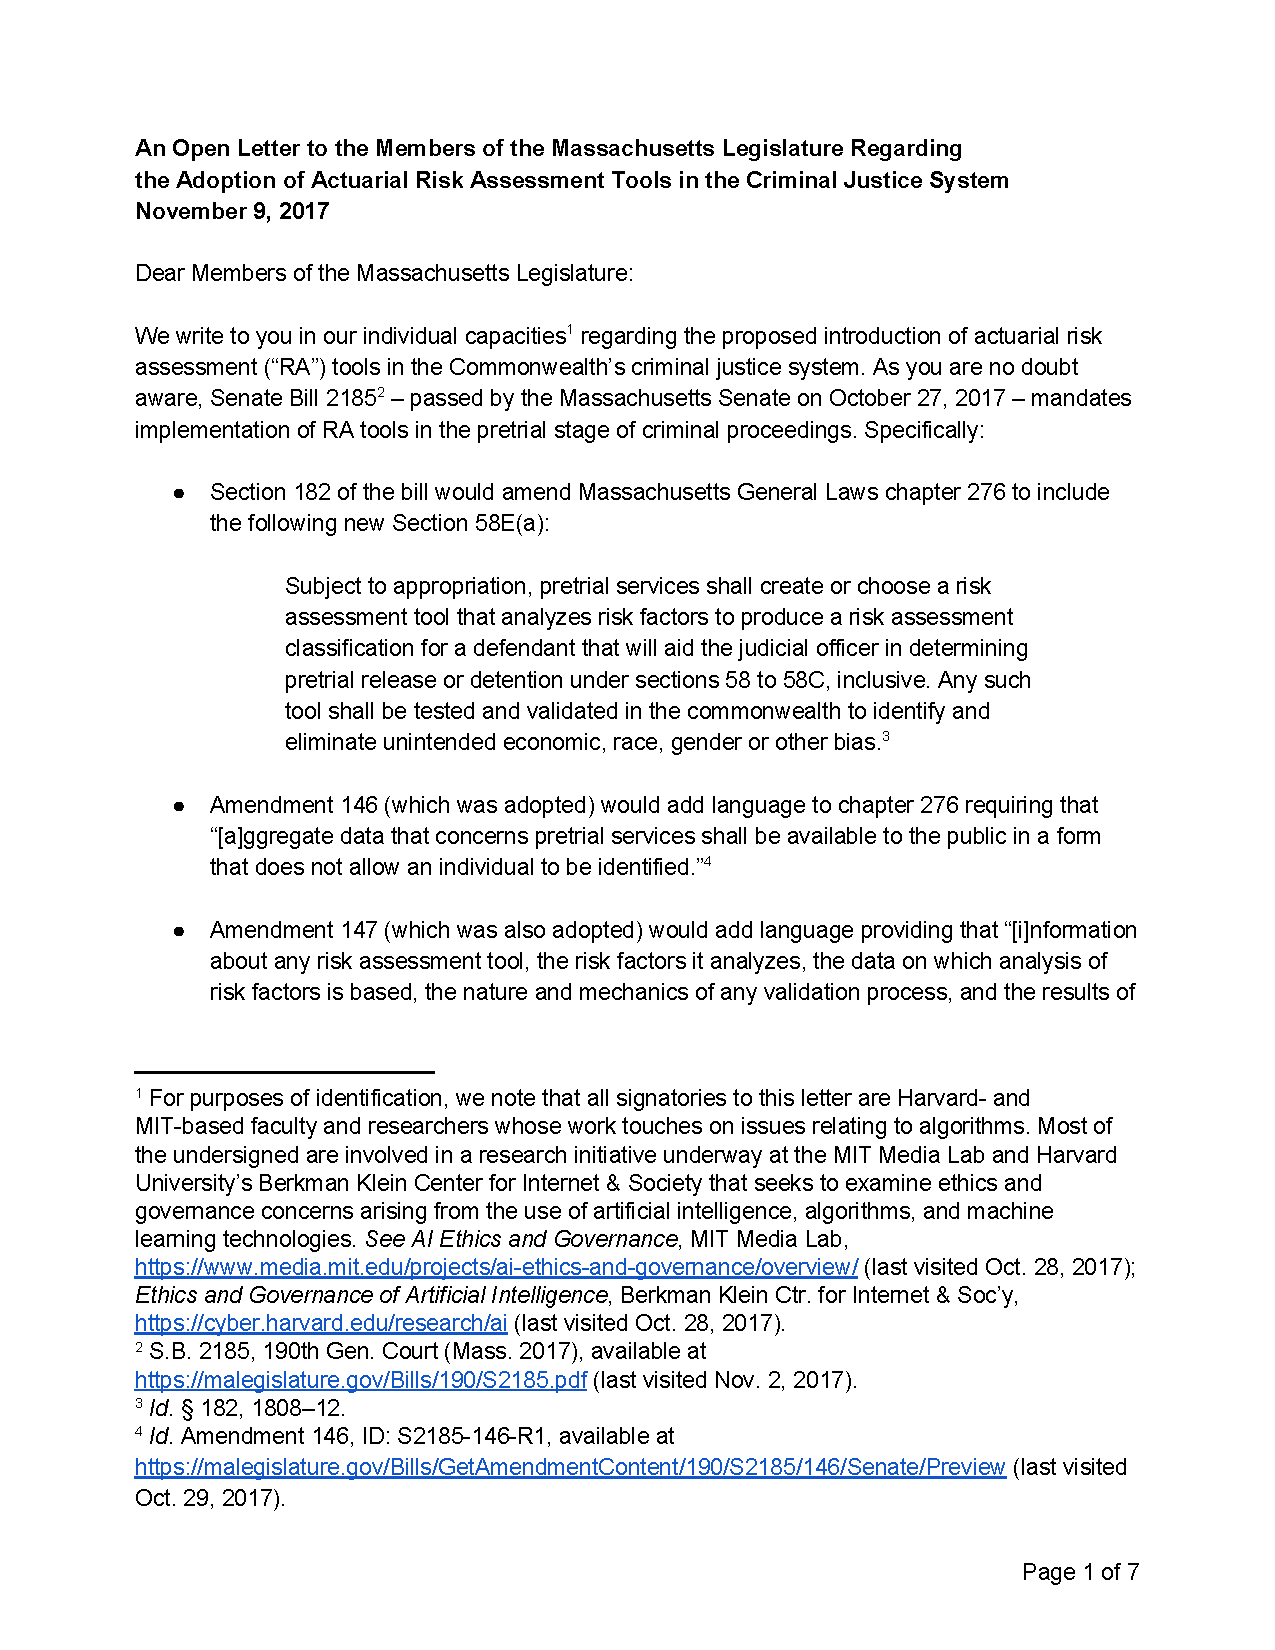
\includepdf[pages=-]{Appendix/Letter-to-MA-Legislature-Nov-9-2017.pdf}
% Appendix C

\chapter{Letter 2 to Massachusetts Legislature On Pretrial Risk Assessments}
\label{appendix:B}

\newpage

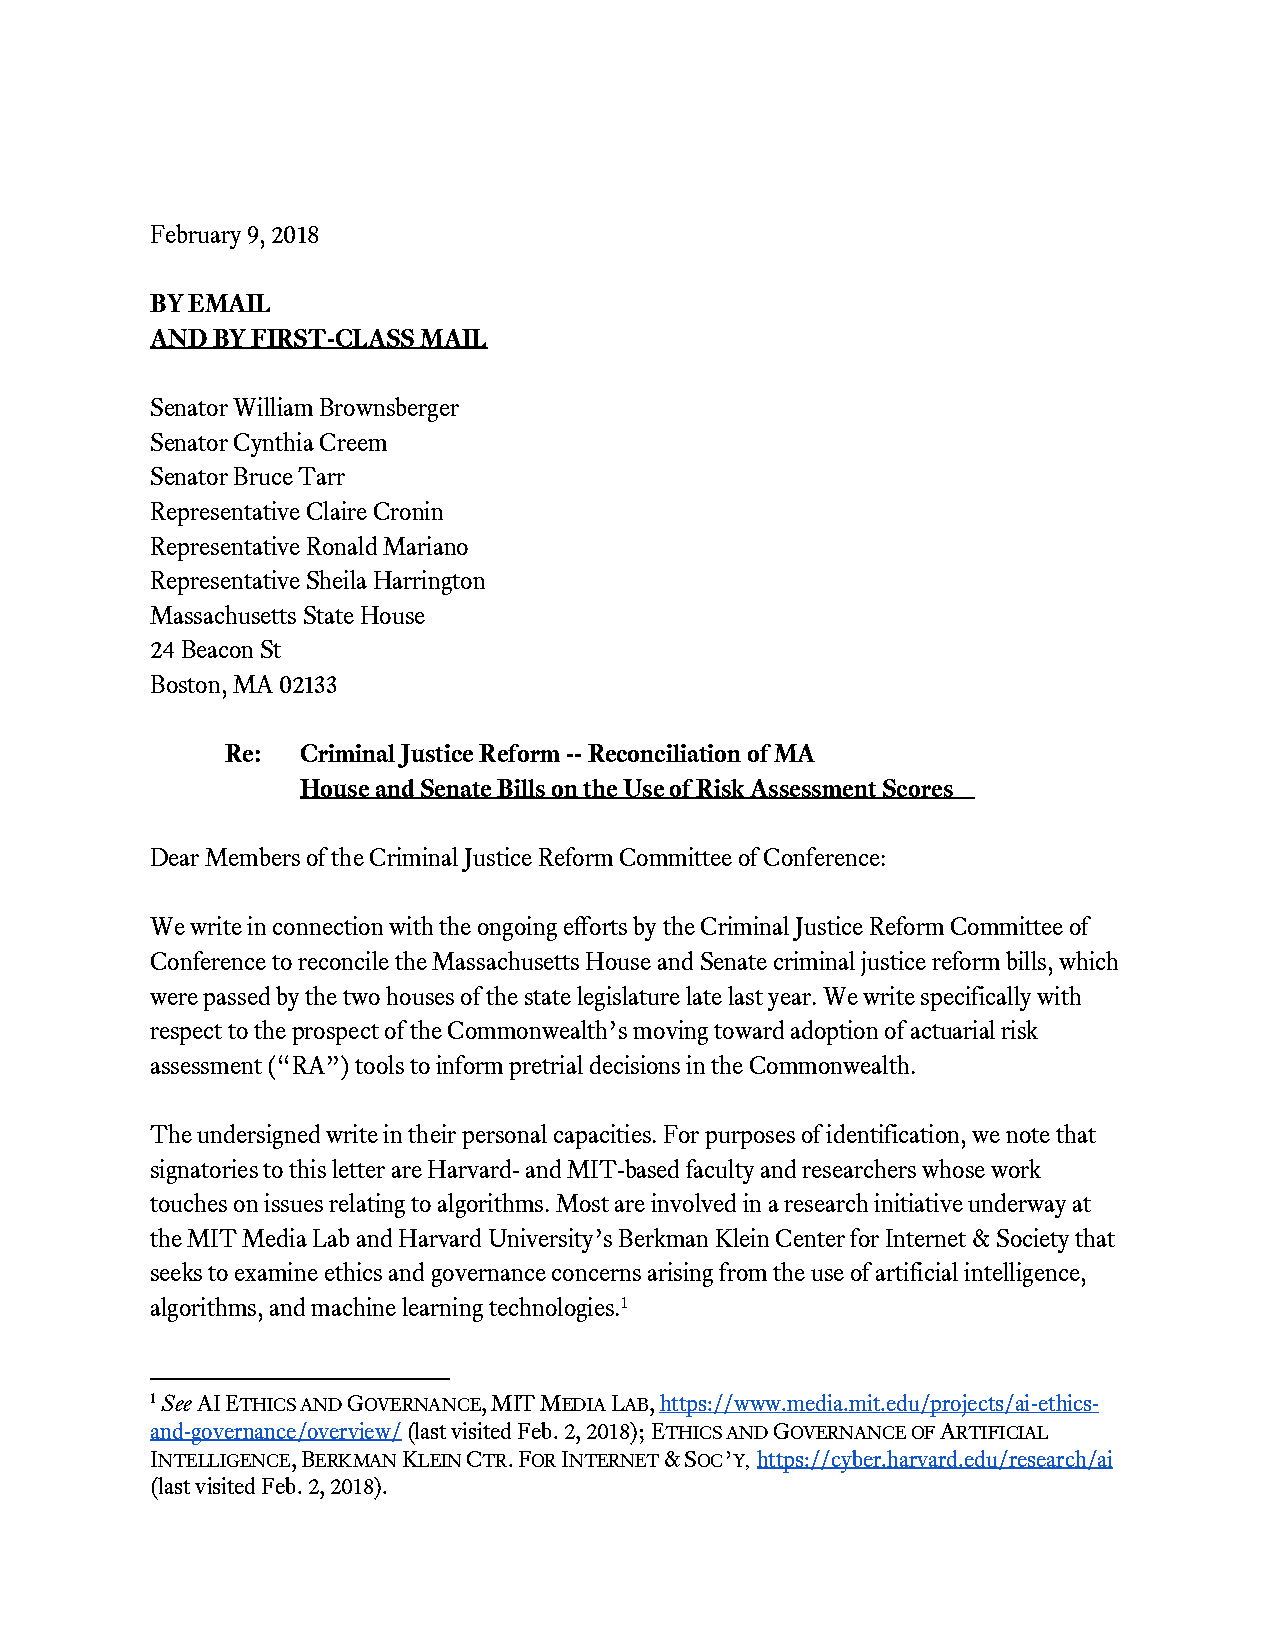
\includepdf[pages=-]{Appendix/Risk-Scoring-Letter-Feb-2018-FINAL-W-Enclosure.pdf}

% Appendix D

\chapter{HavenCo, Ltd. Business Plan}
\label{ch:havenco}

Non-Disclosure: The HavenCo business plan is confidential.  Neither the plan nor any of the information contained herein should be reproduced or disclosed to any person without the written permission of HavenCo.

Disclosure Regarding Forward-Looking Statements: Some of the information provided in the HavenCo Business Plan may contain projections or other forward-looking statements regarding future events or the future financial performance of the Company. We wish to caution you that these statements are only predictions and those actual events or results may differ materially.

Disclosure Regarding Offering: Investment in HavenCo is highly speculative high-risk venture. Only those who can afford to lose their entire investment should respond to the offering. Local laws may affect an investor's ability to participate. Before proceeding with an investment in HavenCo, any potential investor should take care to become familiar with local laws governing investment in foreign corporations, especially any associated reporting requirements, and taxation rules that may apply.

\textbf{Executive Summary}
 
HavenCo, Ltd. is exploiting a unique opportunity to set up the world's first real data haven. The target location is the Principality of Sealand, the world's smallest sovereign territory. HavenCo is building a secure managed co-location business with the added advantage that the customers' data will also be physically secure against any legal actions. Since the co-location business model is a generally profitable one, we expect to continue to be profitable at that site even if a larger nation manages to force some level of regulation over Sealand. HavenCo also intends to use the Sealand operation as a model to demonstrate the profitability of zero-regulation e-commerce to other small countries around the world. We will then be able to eliminate any single point of failure by replicating the "haven" in other jurisdictions. This will also reduce the visibility of our initial showcase site, which will continue to have the best connectivity. HavenCo is currently seeking up to \$3,000,000 in first round funding to establish its showcase data center and begin servicing new customers.

\textbf{PROBLEM / OPPORTUNITY}

The countries that currently have the best infrastructure for e-commerce are suppressing the growth of profitable Internet business through prohibition and regulation of content. Any company that can offer hosting services in a jurisdiction that both allowed free and private data communication and has access to first world bandwidth will have a unique and highly profitable business.


\begin{table}[h]
\centering
\caption[Havenco business plan chart of quality and law-enforcement trade-offs]{Businesses engaged in electronic commerce currently make a fundamental choice to operate from the first-world or the third-world with the following trade-offs.}
\label{havencotable}
\begin{tabular}{lll}
\hline
               & \textbf{First-World}      & \textbf{Third-World}         \\ \hline
Infrastructure & High Quality / Low Cost   & Low Quality / High Cost      \\ \hline
Regulation     & Random / High Enforcement & Negotiable / Low Enforcement \\ \hline
Taxation       & High / High Enforcement   & Negotiable / Low Enforcement \\ \hline
\end{tabular}
\end{table}

It is very difficult, if not impossible, to run businesses which require very high reliability, high-quality infrastructure without regulatory hindrances. Businesses that require high quality e-commerce infrastructure face a significant burden in costs imposed by taxation and regulatory compliance. This prevents many businesses from forming in the first place, and limits the chances of success for those that do start up.

HavenCo will answer the infrastructure vs. freedom question in a fundamentally new way, applying novel technology, a unique physical location, and a world-class team.  We will provide business with better quality infrastructure than ever before, allowing eCommerce operations the luxury of an environment free of unnecessary regulation and taxation, and at a lower total costs than anywhere else.

HavenCo intends to target specifically:

 
\begin{itemize}
\item transaction-oriented businesses, such as electronic gaming, financial and securities systems, and critical business infrastructure such as Application Service Providers (ASPs);
\item security-dependent businesses, such as certificate authorities, records archiving, and security infrastructure businesses;
\item network-centric information-processing businesses (e.g. music, software, graphics, streaming video content, and network infrastructure such as outsourced mail, news, web servers)
\end{itemize}

These market segments fit very well with our potential product and service offerings, and will bring high profitability and rapid growth.  Businesses in these markets face the greatest dilemma in selecting between first-world and third-world infrastructure support. The market is enormous, and growing rapidly, with no competitor providing products and services that simultaneously fulfill all of these customer's needs.

Critical requirements in our target market segments include security (confidentiality, integrity, and availability), transactional performance (primarily driven by latency to the end-user), and ease of use (support existing operating systems and applications).

In order to meet these requirements we will employ several cutting edge or novel technologies.  These include:

\begin{itemize}
\item Ultra-high bandwidth IP communications directly into the Internet backbone (STM-1 to STM-16 and higher), and gigabit-speed internal networks, with superior routing and management
\item Fully redundant power, cooling, network, and management systems, using 2N redundancy when possible
\item Tamper-resistant computing hardware, designed to protect customer transactions from all possible attackers, including HavenCo and its staff
\item Advanced cryptographic protocols to support access control, financial transactions, and secure transaction backup 
\item Open-source software modifications to allow customers to use existing, reliable, well-understood software while exploiting the features of tamper-resistant and cryptographically-secured servers
\end{itemize}

In order to maximize profitability, HavenCo is designing for maximum density, minimum maintenance requirements, believing that a good design and quality equipment will more than pay for itself in reduced labor and overhead and improved quality of service.

In addition to the technologies we will implement and develop to support our core collocation business, HavenCo will be able to use advanced technologies in combination with our unique regulatory situation to offer value-added services never before seen. Such advanced projects will likely include internet-based equities markets and cryptographic token-based payment systems. HavenCo may develop this technology, or partner with others who can already supply it. We will be in an ideal position to market these additional services to our existing customers, and will be able to use them internally as well. It is via such technology that an eventual Internet Public Offering of HavenCo is expected to take place.


\textbf{LOCATION}

A unique asset to HavenCo is the location of its initial showcase data center - the Principality of Sealand. Sealand is the world's smallest sovereign territory. It was founded over thirty years ago, and has obtained a unique legal status as the only sovereign man-made island. Its claim to sovereignty has been tested and supported in several legal challenges.  (See included report on the history and current legal standing of the Principality of Sealand.)

HavenCo does not completely depend upon the continued legal status of Sealand as a de-facto sovereign nation, but is in a position to profit substantially from that status in conjunction with a first-world location. Sealand is located less than 3 milliseconds (by light over fiber) from London, home to leaders in both global finance and international telecommunications. Other than San Jose, California, London is perhaps the world's premier Internet exchange point. Sealand has no laws governing data traffic, and the terms of HavenCo's agreement with Sealand provide that none shall ever be enacted.

In the event that some other nation should manage to successfully exert its jurisdiction over Sealand, the location will continue to provide unique advantages. The legal fight surrounding a challenge o Sealand's sovereignty will provide for a great deal of publicity. If forced to capitulate to a larger nation, it should be possible to leverage Sealand's history and publicity into special status for Sealand. Britain, Sealand's nearest neighbor, is the only real threat in this regard.  It already has many territories with special status and exemptions from many of its laws.

Even if Britain successfully obtained complete control, Sealand would continue to remain a viable location for a secure co-location business. Co-location is a very profitable business model, and we would enter the rapidly expanding market amid a great deal of publicity and attention. This publicity and attention should point to the profitability of our business model, and help us in our plan to replicate the zero-regulation eComerce environment elsewhere.

\textbf{REPLICATION}

The establishment of such the first zero-regulation e-commerce jurisdiction may provoke renewed challenges to Sealand's status. HavenCo therefore plans to replicate this situation as soon as possible at an independent location. Regulatory concerns aside, engineering for redundancy is good systems design policy, and many customers will pay for redundant servers in widely separated physical locations.

Using the publicity and revenues obtained via our Sealand location, we will approach those small governments that are only now just beginning to receive major connectivity to the Internet. The possibility of getting a share of the widely publicized e-commerce marketplace, combined with our demonstration of a working model, should be enough to convince such small governments to establish e-commerce free zones in their countries. Once this begins to happen, our Sealand location will become less unique, and therefore less prone to challenge.

\textbf{TEAM}
    
The HavenCo founders, initial investors, and management consist of experts and visionaries from the network infrastructure, security, and e-commerce industries. Additionally, in spite of the tight global market for technology labor, sufficient staff has already been identified for the first year's operations. We are assisted in filling staffing requirements by both the low manpower needs of the high-density, low-maintenance philosophy, and the fact that our business model holds unique ideological appeal for a fairly large segment of the technology aware community.

In addition to the core team, many vendors are actively participating in a ``build to order'' and financing role, greatly assisting HavenCo in its mission.

HavenCo's founders and core team members include:

\begin{itemize}
\item Sean Hastings --- Chief Executive Officer of HavenCo. Sean was previously CEO of Isle Byte Inc, a Caribbean based consulting company specializing in the development and implementation of hardware and software solutions for telephone and Internet based businesses in offshore jurisdictions. Isle Byte's recent projects have included: the Phone-Book touch-tone telephone and Internet sports betting system for offshore sportsbooks; design of the HOB protocol for SAXAS, an account based eCurrency system being developed by Secure Accounts Ltd, a Caribbean based financial software company; and software development work for Domain Marketplace, a domain registration company for a pacific island Top Level Domain.
\item Jo Hastings --- Chief Marketing Officer of HavenCo. Previously Jo worked as Program Manager for Isle Byte Inc specializing in the set up and operations of Internet casinos from both the Anguilla and California offices. Prior to Isle Byte, she was a Senior Market Analyst for Urban Systems Inc in New Orleans where she edited and wrote for the Gulf South Gaming News, consulted for the Gaming Industry Research Institute of the South and was published in Casino Executive magazine. Her specialty was tribal casinos in the United States as well as emerging technologies for casinos, such as the Internet. She currently sits on the Board of Directors of the Crypto Rights Foundation based in San Francisco.
\item Ryan Lackey --- Chief Technical Officer of HavenCo. Ryan Lackey has worked to bring high security, pro-individual-freedom technologies to the marketplace, first while a student at MIT, and then later in startups developing cryptographic electronic cash solutions for a variety of markets.  Ryan has presented at several conferences and symposia in the security field, and is well known within the security community.
Avi Freedman - Chief Network Architect of HavenCo, also currently VP of Network Architecture for Akamai. Previously he was VP of Engineering for AboveNet. He founded and continues to oversee operations of Netaxs, the first ISP in Philadelphia, founded in 1992. Freedman is also a regular contributor to Boardwatch.
\end{itemize}
 

HavenCo's team of advisors include:

\begin{itemize}
\item Sameer Parekh --- Consultant. Sameer is the well-known founder of C2Net Software, Inc. the leading provider of commercial Apache products and solutions. As CEO of C2Net he pioneered the international offshore cryptography development strategy later adopted by RSA Security in order to deploy strong cryptography worldwide in the face of United States restrictions on the export of strong cryptography. C2Net currently has leading market share in the encrypting web server arena. Sameer is currently a consultant at his own practice known as BPM Consulting International, helping young seed stage startups develop themselves.
\item Joichi Ito --- President of Neotony, a Japanese Internet startup company incubator. Founder of Eccosys, Digital Garage, and InfoSeek Japan. Technical advisor to the Inter-Pacific Bar Association working on a cyber arbitration project. Working with UNCITRAL on rules for arbitration in cyberspace. Working on a committee concerning Japan's position with the WTO and the resolution of transborder legal issues.
\end{itemize}

\textbf{OPERATIONS TO DATE}
 
HavenCo has made substantial progress toward accomplishing its plan.  Since June 1999, HavenCo has done the following:

\begin{itemize}
\item Discovered the possibilities offered by Sealand and made contact with the owners;
\item Visited the Sealand site and inspected it for feasibility of use as a data center;
\item Secured a lease with option to purchase on the \item Sealand facility with highly favorable terms;
\item Assembled a team of experts from the infrastructure and major client industries to conduct operations;
\item Attracted a feature article in the August 2000 issue of Wired magazine, whose editor has said that our story is a good contender for the cover;
\item Developed a technical plan with vendor cooperation to implement a world-class data center at the Sealand facility while requiring minimal capital;
\item Identified and pursued key technologies that support high-quality, highly secure infrastructure;
\item Located several initial sales leads;
\item Concluded agreement for our first pre-sale.
\end{itemize}

\textbf{MILESTONES}

June 1999: Discover Sealand opportunity and begin planning, negotiations, and team formation

November 1999: First site visit and inspection

February 2000: Complete lease/purchase agreements on Sealand; begin accepting investment

March 2000: Conduct engineering tests, establish IP connectivity, local network, initial servers, and begin limited presence on Sealand. Establish London Telehouse presence, routers, transit and peering, and colocation space.

May 2000: Develop sales and marketing materials

June 2000: Pre-position at least 50 servers with at least 45mbps of primary backbone connectivity with backup connectivity.  Target is 100 servers with redundant 155mbps connectivity. Sell at least 10 machines to key customers prior to launch, under nondisclosure, to debug sales and support.

July 2000: Public launch --- publication in Wired, followed by extensive press coverage in general and specialist publications.

August 2000: Seek round two financing from a major network hardware vendor if necessary.

September 2000: Identify possible sites for replication and begin to negotiate with governments in those countries for favorable terms in setting up e-commerce free-zones.  

December 2000: Unit sales of at least 25 major customers.

April 2001: Sign agreement with replication site \#1 and begin construction of second data center. Begin taking pre-sales orders for redundant machine location from current and new customers.

July 2001: Meet sales target for break-even (50 major customers)

December 2001: Internet direct public stock offering

\textbf{PROJECTIONS AND FINANCIAL ANALYSIS}

Given the rapidly-expanding market for transaction servers on the Internet and the modular and infinitely extensible technical plan, HavenCo projects depend critically upon market share. Consequently, we have chosen to pursue the model where we rapidly build market share by offering a superior product at dramatically lower prices than others. However, compared to most ``Internet Businesses,'' we can retain mid-range profitability while following this model, and to the extent required, margins can be cut to meet sales targets, either by reducing costs or (preferably) including additional value added products and services with full-rate core products, while continuing to maintain profitability.

Pro forma financial statements for the first three years of operations are included. The following is a summary of key points:

[REDACTED]

\textbf{THE OFFERING}

Capital is needed to complete initial build out of the Sealand facility and ready it for commercial sales. This funding will be used to develop key technologies to make HavenCo's products and services even more attractive to target markets and to finance sales and marketing efforts.

As a first round of investment, HavenCo, Ltd. Is seeking up to [REDACTED] from angel investors within the infrastructure and client industries via an issue of Series A Preferred Shares. HavenCo, Ltd. will accept investment from individual investors in quantities of [REDACTED] or greater at a price of \$1.54 per share, placing the pre-money valuation of the company at [REDACTED]. This pre-money valuation includes a pool of [REDACTED] shares of common stock reserved for issue to future employees, consultants, and agents.

HavenCo may seek future rounds of financing in order to expand operations, further develop key technologies, and aggressively market its products and services. The extent of future rounds of financing is included in the pro forma financial statements, and is subject to change based on actual revenue levels.

HavenCo eventually plans to offer its shares publicly over the Internet, directly to investors, on its own stock exchange, allowing investors to profit financially, in a timely fashion.  Additionally, due to the superior tax situation afforded by Sealand incorporation, HavenCo may pay dividends without penalty.

 

 
% Appendix E

\chapter{Joi and the Internet in Japan}
\label{chap:jefu}

\textit{by Jeffrey Shapard} \\
\textit{April 2018} \\

This is a personal perspective about how my longtime inspiration, colleague, and friend Joichi Ito influenced the development of the Internet in Japan. It is written in the third-person to create the aura of objectivity, but this is a subjective story. Most of the events and dates and names are true, or close enough, or at least as much as the author can recall in his advancing age and late hour writing. 


\textbf{How it Began: The Seed of Inspiration (1983 or so)}

Back in 1983 or so, Joi was a high school student at the American School in Japan (ASIJ) in western Tokyo and really liked computers. He was in the computer club at his high school. He was active on some early online systems in the US and he was a bit of a hacker, in the exploratory rather than destructive sense. One day he hosted the monthly meeting of the RINGO Club, a user group mostly older expat Americans who had Apple II personal computers, to show them what they could do with an Apple II and an acoustic coupler that let them connect via telephone lines to other computers far away.

Joi fired up his acoustic coupler, dialed a bunch of numbers into his phone, jammed the handset into the coupler, and proceeded to give a worldwide online tour. He started by logging into a couple American online services, CompuServe and The Source, the big boys of the 1980s, to read some forum comments and post a few of his own. Then he logged into a university computer in the UK that hosted a multi-user game he enjoyed. After that he connected out from that university site to hop through a couple more and found a backdoor into some government site, just to show that he could. 

All simple stuff for a young growing up with computers, but it opened up a new world for the older RINGO Club members. One of those RINGO Club members was David G Fisher, a retired US Air Force pilot, longtime resident of Japan, and business and English language educator at the International Education Center in Tokyo and its English language school Nichibei Kaiwa Gakuin. Mr Fisher also liked these new personal computers, and he was always looking for ways to use them in education.

Joi's presentation of online systems stunned him, both in how easy he made it look as well as in the way it opened up the world. Imagine participating in a conversation with people on the other side of the world who were sleeping, but could read your comments and respond later when they woke up. He immediately saw the potential for educational applications.

Mr Fisher had a private student and friend named Toshiaki Tanaka who was president of a shrimp wholesaler and seafood retailer called Sakako Co. Ltd. Tanaka-san also liked personal computers, and was interested in their use for communication and for education. He was using them in his business to consolidate data and to connect his shops, and had hired a very bright game programmer named Makoto Ezure to help set things up. In those days, every Japanese personal computer maker had their own flavor of mostly CP/M-86 operating systems, competing kanji character codes, and very little software. So, Japanese computer users would select their preferred maker and then write their own software. Tanaka-san liked Fujitsu computers and Ezure-san wrote the software for them.

Meanwhile, back at the school where Mr Fisher worked, there had been a drop in attendance so reduced teaching hours were available. The director of the school that specialized in training for business people asked a younger teacher named Jeffrey Shapard if he was willing to do research on educational technology for a couple terms rather than teaching, and he accepted. The director instructed him to hang out with Mr Fisher to get ideas. And so he did.

After a review of various educational software and applications available, and much discussion inspired by what Joi had shown Mr Fisher, the teachers determined that test-taking and quiz applications were far less interesting for language learning that using language to communicate via computer. Mr Fisher then brought Jeffrey to meet Tanaka-san and Ezure-san, and the plan for TWICS as an online system was born.

The plan was presented to the administration of IEC/Nichibei, who agreed to enter into a joint venture with Tanaka-san. Sakako would provide the computers and Ezure-san. IEC/Nichibei would provide Jeffrey and Mr Fisher. And any decisions about eventual commercialization would be joint. The initial purpose was to build a platform for distance learning via online communications.

And the inspiration for this, as Mr Fisher often stated, came from very young Joi, who around that time was graduating from high school and moving off to America to go to college.

\textbf{Pre-Internet days: TWICS (1984-1993)}

In the early 1980s, there were no online services in Japan. By law nobody but the telecom monopoly was allowed to connect anything to the telephone line. There were no modular jacks or handset variations not provided by the monopoly. The only legal way to connect a computer to another via phone line was to use an analog acoustic coupler device, where you had to dial the number by hand, then mash the handset down into phone pads to transmit the relatively slow signal.

There was one personal computer-based bulletin board system (BBS) called CortNet, run by an American named Pete Perkins who operated a computer shop in the Sanno Hotel, which was a US military R\&R facility in central Tokyo. So, legally, those phone lines were US territory, and the US had just recently changed telecom laws to allow individuals to connect devices to the telephone network. CortNet had a modem device that answered the phone automatically, although to get to them one had to dial the Sanno Hotel reception desk and then request a transfer to the computer shop to get the modem to answer. It was cumbersome, really rattled the reception desk staff, but was totally amazing to first time online users.

Tanaka-san told Ezure-san not the break the law, so in addition to building the BBS-inspired software application for the Fujitsu personal computer platform, Ezure-san also had to fabricate a Rube Goldberg device involving acoustic couplers and a controller attached to wiring in the phone (not to the line) to answer and hang up calls. The first TWICS online system launched in 1984, hosted by 2 networked Fujitsu personal computers and 2 acoustic couplers for two simultaneous online users. It was then either the first or second BBS in Japan other than CortNet, and depending on claims about who went live earlier in one 24-hour period. The other BBS was set up by a local expat PC user club using computers, software, and modems imported from the US, the latter illegal by Japanese law, and for the purpose of talking tech and swapping bootleg software.

TWICS was named by Tanaka-san, who was bearing most of the costs. He wanted it to mean “Two Way Information and Communication System”, although when his accountant registered the name and rendered it into a Japanese pronunciation, it got really mangled. And Tanaka-san operated with the brand Honeymoon for his shrimp, and bees make honey, and honey makes people happy, so he wanted our logo and motif to involve bees. Hence, the official full name TWICS BeeLine. It all made sense at the time.

And then Joi came home from school for the summer and joined TWICS. Jeffrey had been in email communication with him via The Source and they had been exploring how to set things up for TWICS to be a more relevant platform than a BBS, with communications more meaningful than shallow chatter, and with a way for groups, classes, teams, communities to evolve online. There seemed to be no terms that captured what they were doing: pasocom tsuushin (PC communications), going online, computer conferencing, electronic networking. The few people doing it in those days understood it, but it was very difficult to explain to others, and therefore a challenge to promote and grow.

Joi became an advisor and member of the TWICS team. He had experience on various other systems, and helped get conversations and momentum going on that first system that got beyond the shallow chatter of most of the BBS world of that era. And he helped the team understand that it is not necessarily about the technical platform, but more about how it is applied. It is all about the application and the people, not the technology.

Then Joi went back to America for school for a while. In 1985 TWICS outgrew 2 phone lines and, in a crash development marathon, built and launched a new software platform on Unix-based host computer, with new applications for email and the forums, and fancy new higher speed modems connected directly to the phone lines. The laws had started to change and TWICS expanded to 4 lines. However, the host computer proved inadequate for the task and the team was distracted by having to build and support all the software, which distracted from the focus on communications, groups, classes, and the emerging virtual community.

Then Joi came back to Japan again, this time to stay longer. He advised the TWICS team to get out of the software writing business, obtain some decent software for a reliable platform, and focus on the application and service, not the technology. And so they did.

After a survey of what was available, they selected PARTICIPATE, the software application for computer conferencing used on the big American online service called The Source, and a DEC MicroVAX II running the VMS operating system to support it. This time the software drove the hardware decision. In addition to the 6 phone lines, the TWICS system was connected to a couple X.25 networks as alternative to long-distance dialing for users beyond Tokyo, and beyond Japan. TWICS went global.

By then Jeffrey had become the system administrator. He challenged Joi to hack into the system. He tried, and would eventually have succeeded, so Jeffrey gave him full root administrator privileges because he would have figured out how to get them anyway.

Joi became an active member of the TWICS online community and inspired others. Joi started a monthly meeting for people interested in telecommunications with personal computers called T-Net, where he often presented telecom tricks and techniques, or gave tours and demonstrated things on other systems, and generally shared his knowledge. Many TWICS members came to T-Net and what became the traditional lunch and Saturday afternoon party at an Indonesian restaurant down the street. Some of those participants in the T-Net meetings went on to start other online services or spread the use of the technology into the businesses and organizations.

This combination of a virtual community with regular opportunities to actually meet other members face to face became a critical feature of the community, and more important as Joi invited in other folks he know from his global networking travels to become guest members of TWICS. Eventually there were members coming in from 25+ countries before the Internet made it all so much easier and cheaper, and it was common to have international visitors drop by for the monthly meetings. This created a unique educational opportunity for the Japanese members, and created context for real experience using English in real communications with real people.

But the Internet was coming. In 1990 or so, Jun Murai, the founder of the Japanese academic network JUNet, gave a presentation to the International Computer Association and said that their academic network was open to commercial entities, if interested. Jeffrey pounced and asked Murai-san to let TWICS connect to JUNet. Within a couple weeks, TWICS had an Internet domain name (twics.co.jp) and a dialup uucp connection to a JUNet host computer for distributed email and news groups.

But international telecom rules in Japan made it difficult for Internet connectivity beyond Japan for anything but academic purposes. Meanwhile across the Pacific in the US, the Internet had escaped academia and begun commercial development.


\textbf{Intro of the Internet: IIKK (1993)}

Jeffrey left Japan in 1992 and returned to the US for business school. He was contracted by a US software firm called Intercon during the summer of 1993 to go back to Japan and help their Japanese joint venture partner set up an Internet access business. They had one commercial customer already waiting for them.

After several weeks trying to gain access to the old karaoke bar that was to be used for the office of the new Internet venture, in the final week Jeffrey and his small start-up team of his wife Masaji and classmate Bill Hodgson got the new company incorporated, got license approval from the Ministry of Posts \& Telecoms, and recruited a local manager and staff. The company was registered as Intercon International KK, with internet domain “iikk.co.jp". The company had also managed to register the domain “inter.net”. For various reasons, nobody else had. 

However, before the network service could be set up and made operational, an ownership dispute between Intercon and their local joint venture partner got the start-up team kicked out of their karaoke bar office.

Jeffrey went to Joi for ideas, and Joi found IIKK a room for an office and a spare bathroom in a condo next to where he had his office.

A dedicated international circuit for Internet access service was pulled into the spare bathroom, and a router and server were installed in a small rack in the shower stall for the access point. The first commercial Internet access point in Japan was in a shower stall! An ethernet cable was strung out the window and over into Joi's window for his Internet access, and his office became the first non-academic site in Japan connected to the international Internet when the service went live.

The first commercial customer of IIKK was TWICS, whose local community was one of the first in Japan connected directly to the Internet, and whose service rapidly expanded as one of the first dial-up Internet access providers.

Jeffrey left Tokyo and returned to the US and Joi continued to support the fledging Internet access business.

At the end of 1993, Intercon decided to sell IIKK to PSINet, one of the pioneers in the commercial Internet business in the US. Jeffrey returned to Japan with Bill Schrader, the president of PSINet, for due diligence before the final decision and Joi was the first person he met in Japan the night he arrived. PSINet acquired IIKK, fired the local manager, and put in place a new team that would become PSINet Japan.


\textbf{Building the Internet: PSINet Japan (1994-2000)}

Joi continued to provide moral and opportunity support to the local technical employees Vince Gebes and Eric Bowles and a series of American managers. The business grew slowly due to marketing and sales constraints, but Vince began to emerge as team leader. However, he was an engineer and not yet ready to build a business.

In the meantime, PSINet went public in the US in 1995 and began to expand their network infrastructure and business operations rapidly across the US and Canada, and made a new acquisition in the UK. In 1996 they turned their attention back to PSINet Japan.

The PSINet executive team wanted a seasoned ``industry professional'' to build the company, even though the Internet was yet a nascent industry with a business model that would basically disrupt all the established industries it touched. They thought they wanted an old school manager but they needed an agent of change.

So, despite the objections of some other executives, PSINet CEO Bill Schrader called Joi and asked him to lead PSINet Japan as President. He knew that Joi had another business, various other projects in motion, maybe a board or official committee seat or two and various other time conflicts, and was not much of an operational manager. But he was a player not afraid to be bold, he quickly understood the ambition in the PSINet ambition, and he saw how everything was connected.

Joi was interested in everything, he knew everybody, he was enthusiastic, and he agreed to help PSINet get to the next level in Japan. And this time he actually got paid for his support.

Joi moved the company from their crowded condo space to a nice office in Akasaka, got the team all excited about fast growth, and hired a party space for a big coming out party. He invited the shakers and movers in the technology, media and emerging Internet businesses, then followed through with a public relations blitz and media interviews. He rebuilt critical relationships that had been neglected, initiated new ones needed to move forward, and promoted the Internet everywhere.

Basically, Joi put PSINet on the map in Japan. Then he handed off ongoing marketing and business growth to Vince and their growing team, and departed for other ventures.

PSINet Japan continued on the trajectory set by Joi, with bold marketing, impact beyond their size, and a willingness to try new things. Vince became the next president, and within a few years as PSINet raised even more money, they acquired three more Internet companies in Japan, including TWICS where it all began, and became the headquarters for PSINet in the Asia Pacific region where numerous other Internet service providers were acquired in other countries. It was a time of great expansion.

Alas, one day investors woke up caring more about profitability than expansion in the now booming but overheated Internet industry, and by 2000 PSINet had crashed and burned and was sold off in pieces. PSINet Japan operations were acquired and integrated into another telecoms company in Japan.

Vince and Eric and other colleagues from PSINet Japan, including Tim Burress from TWICS, went on to found a successful Internet security services business.

\textbf{From a Seed to the Internet}

Had Joi not shared his early online experience as a teenager with a bunch of early Apple II hobbyists in Tokyo in 1983 or so, there would have been no TWICS and IIKK and early PSINet Japan. The Internet would still have emerged in Japan without pioneering Joi and his American friends, but more slowly and perhaps in a more insular and regulated manner.

Joi did not specifically build the day-to-day operations of TWICS or even PSINet Japan, but was somehow always there at key times to influence development or give things a nudge in some new direction, whether as a community member, a friend and free consultant, an advisor to the board, or as company president. Or maybe those times became key because he was there.

Joi influenced the Internet in Japan by connecting people and ideas early and significantly, by asking creative questions, and by constantly promoting a vision of the potential of trying new things and new ways.


% Appendix F
\chapter{Nia Tero Preamble}
\label{appendix:niatero}

\newpage


\includepdf[pages=-,scale=0.85,offset=20mm 0mm]{Appendix/NiaTeroPreamble050418BdMtg.pdf}

% Appendix G

\chapter{Health 0.0}
\label{appendix:health}

\textbf{Readouts and reports from individual workshops:} \\

% Workshop 1
\textbf{Workshop 1: October 7th 2016.}
 
A group of Life sciences professionals held a one-day meeting with the MIT Media Lab to discuss the potential to develop a new paradigm for drug development. The meeting examined a new drug development approach, which is prompted by a changing healthcare environment resulting from the adoption of new technologies.

It was proposed, that the following factors need to be considered:
\begin{itemize}
\item Pharmaceutical Industry, Providers and Payers would have to develop a robust, consistent and dynamic data sharing environment
\item Clarity would be needed on who owns data and how broad access is achieved to accelerate research
\item New incentive models would need to be developed across multiple stakeholders in the clinical trial ecosystem to ensure strong participation and data sharing
\item A new paradigm on potential liability will need to be introduced requiring new models of indemnification (e.g. joint liabilities)
\item Regulators would have to be open to the new model and build the associated needed capabilities and resources
\end{itemize}

Overall the group, felt that the development of a new model was worth further exploration and that other interested parties should be engaged. It should be noted that if the new model were successful, it would have potential benefits for the patient and key stakeholders. The team should also assess what other efforts are being pursued on this topic by other entities e.g. NewDigs, EMEA, Transcelerate etc.

Full report from the workshop: \href{https://drive.google.com/file/d/1kFMbGtNa5IxEZz02Qn8uw-oOeWQ1qIiq/view}{Workshop 1 full report} \\

% Workshop 2
\textbf{Workshop 2: March 17th 2017}

A group of Life sciences professionals from member companies held a 1-day meeting with MIT Media Lab to discuss approaches to apply and develop new Machine Learning (ML) and Deep Neural Networks (DNNs) for classification of clinical and pharmaceutical research data. Pratik Shah from the Media Lab presented a two-hour overview of the current state of Artificial Intelligence (AI) in computer science and related fields, followed by five case studies of emergent AI for classification of clinical and biological data.  Francis Kendall from Roche and representatives from Biogen, Microsoft, Medimmune and VSP then shared individual case studies, challenges and machine learning approaches being used in their respective companies.Three potential areas for engagement with the Media Lab and other member companies were discussed:
1) New algorithms for automated structuring of raw biological data for input into ML and DNN classifiers by bioinformatics and data science professionals;
2) Develop new models and emerging DNN architectures for classification of multimodal clinical and biological datasets
3) How do we build a horizontal pharma/bio data platform that all media lab member companies can contribute to and get value from? There is sustainable interest from the Media Lab pharma companies to continue similar workshops to discuss the intersection between AI and drug discovery, but for logistical reasons these will be combined with the regulatory drug discovery  workshops. \\
 
\textbf{Key recommendations and agreed actions}
\begin{enumerate}
\item a. Publish key challenges of the new approach to start a dialogue for the wider community to solve \\
b. Data – Explore the feasibility of an Open Data Model \\
c. Develop collaboration experimentation e.g. Sharing data. \\
d. Predictability - How Might We apply AI/Machine Learning to enhance the process?
\item Additional examples of published successful DNN/ML approaches to be shared with team
\item Pharmaceutical company representatives will explore opportunities to identify and agree on a data collaboration study
\item Explore and link to ongoing conversations and initiatives on the new paradigm for clinical development theme.
\end{enumerate}

Full report from the workshop: \href{https://drive.google.com/file/d/1l1dgWlCuBms-LWHdrP6-4qDdLJs83fkq/view?usp=sharing}{Workshop 2 full report} \\

% Workshop 4
\textbf{Workshop 4: October 10th 2017}

The morning was a forum with presentations various topics related to engendering a new digital paradigm for the future of health and drug development. Speakers from pharma, health, technology Media Lab Member companies and the FDA participated. The afternoon will include a workshop facilitated by The Boston Consulting Group where speakers and guests can brainstorm. Followed by an executive meeting of key leaders and speakers from various organizations to chart out next steps:
Objectives included:
\begin{itemize}
\item Developing a sustainable model to bridge the gap between AI and data science experts and the life sciences community
\item Addressing current, near-term AI, machine learning, and neural network capabilities as they pertain to drug development
\item Identifying new AI inventions and data structures that can solve key drug development challenges
\item Identifying collaborations around use cases for existing AI to solve high-impact drug development challenges
\item Discussing roadblocks limiting the full potential of AI in drug development
\end{itemize}

Final workshop agenda: \href{https://www.media.mit.edu/events/artificial-intelligence-in-clinical-development-to-improve-public-health/}{Workshop 3 agenda}

\textit{Key action items from this workshop (listed below) are been prepared in the form of a Perspective article to be submitted to Nature Reviews Drug Discovery} \\

% TODO
\textbf{Key outcomes and next steps:}

\begin{enumerate}
\item The first priority is data aggregation an availability
\begin{itemize}
\item e.g. Common hurdle: Significantly limited amount of high-quality, sufficiently large datasets (especially for AI training)
\item Potential approaches: Members can start by contributing legacy "abandoned project" or pre-competitive, masked datasets; unstructured and structured data should be collected and pre-processed; new data capture standards (format, access etc.) should be defined
\end{itemize}

\item AI can be used for aggregation AND (retrospective and prospective) analytics
\begin{itemize}
\item AI is not just for analysis, but also for data pre-processing/aggregation
\item Confidentiality or competition-sensitive concerns can be addressed using a decentralized aggregation and analysis approach
\item Incentivisation between the AI and Pharma community needs to find common ground to accelerate collaboration
\item Analytics should include retrospective analysis and efforts to capture new, novel and better suited data to enable prospective analysis
\item A focus is needed on pervasive, foundational enablers in order to truly enable use of AI
\item We should shift our conversations to include AI when we talk about Digital Health and RWD – it's all about data and solution ecosystems
e.g. Pervasive integration of Digital Health tools along the care journey ("at scale"), i.e. point of care to real world setting
\item Pharma and Payer members to identify Digital Health integration points along the care journey in which to embed Digital Health tools for the purpose of, but not limited, enhanced data collection to enable extensive feature rich datasets for AI-based analytics
\item Standardized analytical approaches are uncommon and transparency on approaches is limited
\item Multi-stakeholder alignment, awareness, education activities and ethics discussions are required to realize the adoption, integration and ideal leverage of AI in Clinical Development and healthcare in general
\item Conservatism and the need for education and alignment for regulators, payers, clinicians, and patients (vs. ``black box'' problem, acceptance of non-traditional measures)
\item Roles of ethics associated with AI in healthcare, especially in Pharma setting, needs to be more clearly explored and defined
\end{itemize}
\end{enumerate}
% % Appendix D

\chapter{HavenCo, Ltd. Business Plan}
\label{ch:havenco}

Non-Disclosure: The HavenCo business plan is confidential.  Neither the plan nor any of the information contained herein should be reproduced or disclosed to any person without the written permission of HavenCo.

Disclosure Regarding Forward-Looking Statements: Some of the information provided in the HavenCo Business Plan may contain projections or other forward-looking statements regarding future events or the future financial performance of the Company. We wish to caution you that these statements are only predictions and those actual events or results may differ materially.

Disclosure Regarding Offering: Investment in HavenCo is highly speculative high-risk venture. Only those who can afford to lose their entire investment should respond to the offering. Local laws may affect an investor's ability to participate. Before proceeding with an investment in HavenCo, any potential investor should take care to become familiar with local laws governing investment in foreign corporations, especially any associated reporting requirements, and taxation rules that may apply.

\textbf{Executive Summary}
 
HavenCo, Ltd. is exploiting a unique opportunity to set up the world's first real data haven. The target location is the Principality of Sealand, the world's smallest sovereign territory. HavenCo is building a secure managed co-location business with the added advantage that the customers' data will also be physically secure against any legal actions. Since the co-location business model is a generally profitable one, we expect to continue to be profitable at that site even if a larger nation manages to force some level of regulation over Sealand. HavenCo also intends to use the Sealand operation as a model to demonstrate the profitability of zero-regulation e-commerce to other small countries around the world. We will then be able to eliminate any single point of failure by replicating the "haven" in other jurisdictions. This will also reduce the visibility of our initial showcase site, which will continue to have the best connectivity. HavenCo is currently seeking up to \$3,000,000 in first round funding to establish its showcase data center and begin servicing new customers.

\textbf{PROBLEM / OPPORTUNITY}

The countries that currently have the best infrastructure for e-commerce are suppressing the growth of profitable Internet business through prohibition and regulation of content. Any company that can offer hosting services in a jurisdiction that both allowed free and private data communication and has access to first world bandwidth will have a unique and highly profitable business.


\begin{table}[h]
\centering
\caption[Havenco business plan chart of quality and law-enforcement trade-offs]{Businesses engaged in electronic commerce currently make a fundamental choice to operate from the first-world or the third-world with the following trade-offs.}
\label{havencotable}
\begin{tabular}{lll}
\hline
               & \textbf{First-World}      & \textbf{Third-World}         \\ \hline
Infrastructure & High Quality / Low Cost   & Low Quality / High Cost      \\ \hline
Regulation     & Random / High Enforcement & Negotiable / Low Enforcement \\ \hline
Taxation       & High / High Enforcement   & Negotiable / Low Enforcement \\ \hline
\end{tabular}
\end{table}

It is very difficult, if not impossible, to run businesses which require very high reliability, high-quality infrastructure without regulatory hindrances. Businesses that require high quality e-commerce infrastructure face a significant burden in costs imposed by taxation and regulatory compliance. This prevents many businesses from forming in the first place, and limits the chances of success for those that do start up.

HavenCo will answer the infrastructure vs. freedom question in a fundamentally new way, applying novel technology, a unique physical location, and a world-class team.  We will provide business with better quality infrastructure than ever before, allowing eCommerce operations the luxury of an environment free of unnecessary regulation and taxation, and at a lower total costs than anywhere else.

HavenCo intends to target specifically:

 
\begin{itemize}
\item transaction-oriented businesses, such as electronic gaming, financial and securities systems, and critical business infrastructure such as Application Service Providers (ASPs);
\item security-dependent businesses, such as certificate authorities, records archiving, and security infrastructure businesses;
\item network-centric information-processing businesses (e.g. music, software, graphics, streaming video content, and network infrastructure such as outsourced mail, news, web servers)
\end{itemize}

These market segments fit very well with our potential product and service offerings, and will bring high profitability and rapid growth.  Businesses in these markets face the greatest dilemma in selecting between first-world and third-world infrastructure support. The market is enormous, and growing rapidly, with no competitor providing products and services that simultaneously fulfill all of these customer's needs.

Critical requirements in our target market segments include security (confidentiality, integrity, and availability), transactional performance (primarily driven by latency to the end-user), and ease of use (support existing operating systems and applications).

In order to meet these requirements we will employ several cutting edge or novel technologies.  These include:

\begin{itemize}
\item Ultra-high bandwidth IP communications directly into the Internet backbone (STM-1 to STM-16 and higher), and gigabit-speed internal networks, with superior routing and management
\item Fully redundant power, cooling, network, and management systems, using 2N redundancy when possible
\item Tamper-resistant computing hardware, designed to protect customer transactions from all possible attackers, including HavenCo and its staff
\item Advanced cryptographic protocols to support access control, financial transactions, and secure transaction backup 
\item Open-source software modifications to allow customers to use existing, reliable, well-understood software while exploiting the features of tamper-resistant and cryptographically-secured servers
\end{itemize}

In order to maximize profitability, HavenCo is designing for maximum density, minimum maintenance requirements, believing that a good design and quality equipment will more than pay for itself in reduced labor and overhead and improved quality of service.

In addition to the technologies we will implement and develop to support our core collocation business, HavenCo will be able to use advanced technologies in combination with our unique regulatory situation to offer value-added services never before seen. Such advanced projects will likely include internet-based equities markets and cryptographic token-based payment systems. HavenCo may develop this technology, or partner with others who can already supply it. We will be in an ideal position to market these additional services to our existing customers, and will be able to use them internally as well. It is via such technology that an eventual Internet Public Offering of HavenCo is expected to take place.


\textbf{LOCATION}

A unique asset to HavenCo is the location of its initial showcase data center - the Principality of Sealand. Sealand is the world's smallest sovereign territory. It was founded over thirty years ago, and has obtained a unique legal status as the only sovereign man-made island. Its claim to sovereignty has been tested and supported in several legal challenges.  (See included report on the history and current legal standing of the Principality of Sealand.)

HavenCo does not completely depend upon the continued legal status of Sealand as a de-facto sovereign nation, but is in a position to profit substantially from that status in conjunction with a first-world location. Sealand is located less than 3 milliseconds (by light over fiber) from London, home to leaders in both global finance and international telecommunications. Other than San Jose, California, London is perhaps the world's premier Internet exchange point. Sealand has no laws governing data traffic, and the terms of HavenCo's agreement with Sealand provide that none shall ever be enacted.

In the event that some other nation should manage to successfully exert its jurisdiction over Sealand, the location will continue to provide unique advantages. The legal fight surrounding a challenge o Sealand's sovereignty will provide for a great deal of publicity. If forced to capitulate to a larger nation, it should be possible to leverage Sealand's history and publicity into special status for Sealand. Britain, Sealand's nearest neighbor, is the only real threat in this regard.  It already has many territories with special status and exemptions from many of its laws.

Even if Britain successfully obtained complete control, Sealand would continue to remain a viable location for a secure co-location business. Co-location is a very profitable business model, and we would enter the rapidly expanding market amid a great deal of publicity and attention. This publicity and attention should point to the profitability of our business model, and help us in our plan to replicate the zero-regulation eComerce environment elsewhere.

\textbf{REPLICATION}

The establishment of such the first zero-regulation e-commerce jurisdiction may provoke renewed challenges to Sealand's status. HavenCo therefore plans to replicate this situation as soon as possible at an independent location. Regulatory concerns aside, engineering for redundancy is good systems design policy, and many customers will pay for redundant servers in widely separated physical locations.

Using the publicity and revenues obtained via our Sealand location, we will approach those small governments that are only now just beginning to receive major connectivity to the Internet. The possibility of getting a share of the widely publicized e-commerce marketplace, combined with our demonstration of a working model, should be enough to convince such small governments to establish e-commerce free zones in their countries. Once this begins to happen, our Sealand location will become less unique, and therefore less prone to challenge.

\textbf{TEAM}
    
The HavenCo founders, initial investors, and management consist of experts and visionaries from the network infrastructure, security, and e-commerce industries. Additionally, in spite of the tight global market for technology labor, sufficient staff has already been identified for the first year's operations. We are assisted in filling staffing requirements by both the low manpower needs of the high-density, low-maintenance philosophy, and the fact that our business model holds unique ideological appeal for a fairly large segment of the technology aware community.

In addition to the core team, many vendors are actively participating in a ``build to order'' and financing role, greatly assisting HavenCo in its mission.

HavenCo's founders and core team members include:

\begin{itemize}
\item Sean Hastings --- Chief Executive Officer of HavenCo. Sean was previously CEO of Isle Byte Inc, a Caribbean based consulting company specializing in the development and implementation of hardware and software solutions for telephone and Internet based businesses in offshore jurisdictions. Isle Byte's recent projects have included: the Phone-Book touch-tone telephone and Internet sports betting system for offshore sportsbooks; design of the HOB protocol for SAXAS, an account based eCurrency system being developed by Secure Accounts Ltd, a Caribbean based financial software company; and software development work for Domain Marketplace, a domain registration company for a pacific island Top Level Domain.
\item Jo Hastings --- Chief Marketing Officer of HavenCo. Previously Jo worked as Program Manager for Isle Byte Inc specializing in the set up and operations of Internet casinos from both the Anguilla and California offices. Prior to Isle Byte, she was a Senior Market Analyst for Urban Systems Inc in New Orleans where she edited and wrote for the Gulf South Gaming News, consulted for the Gaming Industry Research Institute of the South and was published in Casino Executive magazine. Her specialty was tribal casinos in the United States as well as emerging technologies for casinos, such as the Internet. She currently sits on the Board of Directors of the Crypto Rights Foundation based in San Francisco.
\item Ryan Lackey --- Chief Technical Officer of HavenCo. Ryan Lackey has worked to bring high security, pro-individual-freedom technologies to the marketplace, first while a student at MIT, and then later in startups developing cryptographic electronic cash solutions for a variety of markets.  Ryan has presented at several conferences and symposia in the security field, and is well known within the security community.
Avi Freedman - Chief Network Architect of HavenCo, also currently VP of Network Architecture for Akamai. Previously he was VP of Engineering for AboveNet. He founded and continues to oversee operations of Netaxs, the first ISP in Philadelphia, founded in 1992. Freedman is also a regular contributor to Boardwatch.
\end{itemize}
 

HavenCo's team of advisors include:

\begin{itemize}
\item Sameer Parekh --- Consultant. Sameer is the well-known founder of C2Net Software, Inc. the leading provider of commercial Apache products and solutions. As CEO of C2Net he pioneered the international offshore cryptography development strategy later adopted by RSA Security in order to deploy strong cryptography worldwide in the face of United States restrictions on the export of strong cryptography. C2Net currently has leading market share in the encrypting web server arena. Sameer is currently a consultant at his own practice known as BPM Consulting International, helping young seed stage startups develop themselves.
\item Joichi Ito --- President of Neotony, a Japanese Internet startup company incubator. Founder of Eccosys, Digital Garage, and InfoSeek Japan. Technical advisor to the Inter-Pacific Bar Association working on a cyber arbitration project. Working with UNCITRAL on rules for arbitration in cyberspace. Working on a committee concerning Japan's position with the WTO and the resolution of transborder legal issues.
\end{itemize}

\textbf{OPERATIONS TO DATE}
 
HavenCo has made substantial progress toward accomplishing its plan.  Since June 1999, HavenCo has done the following:

\begin{itemize}
\item Discovered the possibilities offered by Sealand and made contact with the owners;
\item Visited the Sealand site and inspected it for feasibility of use as a data center;
\item Secured a lease with option to purchase on the \item Sealand facility with highly favorable terms;
\item Assembled a team of experts from the infrastructure and major client industries to conduct operations;
\item Attracted a feature article in the August 2000 issue of Wired magazine, whose editor has said that our story is a good contender for the cover;
\item Developed a technical plan with vendor cooperation to implement a world-class data center at the Sealand facility while requiring minimal capital;
\item Identified and pursued key technologies that support high-quality, highly secure infrastructure;
\item Located several initial sales leads;
\item Concluded agreement for our first pre-sale.
\end{itemize}

\textbf{MILESTONES}

June 1999: Discover Sealand opportunity and begin planning, negotiations, and team formation

November 1999: First site visit and inspection

February 2000: Complete lease/purchase agreements on Sealand; begin accepting investment

March 2000: Conduct engineering tests, establish IP connectivity, local network, initial servers, and begin limited presence on Sealand. Establish London Telehouse presence, routers, transit and peering, and colocation space.

May 2000: Develop sales and marketing materials

June 2000: Pre-position at least 50 servers with at least 45mbps of primary backbone connectivity with backup connectivity.  Target is 100 servers with redundant 155mbps connectivity. Sell at least 10 machines to key customers prior to launch, under nondisclosure, to debug sales and support.

July 2000: Public launch --- publication in Wired, followed by extensive press coverage in general and specialist publications.

August 2000: Seek round two financing from a major network hardware vendor if necessary.

September 2000: Identify possible sites for replication and begin to negotiate with governments in those countries for favorable terms in setting up e-commerce free-zones.  

December 2000: Unit sales of at least 25 major customers.

April 2001: Sign agreement with replication site \#1 and begin construction of second data center. Begin taking pre-sales orders for redundant machine location from current and new customers.

July 2001: Meet sales target for break-even (50 major customers)

December 2001: Internet direct public stock offering

\textbf{PROJECTIONS AND FINANCIAL ANALYSIS}

Given the rapidly-expanding market for transaction servers on the Internet and the modular and infinitely extensible technical plan, HavenCo projects depend critically upon market share. Consequently, we have chosen to pursue the model where we rapidly build market share by offering a superior product at dramatically lower prices than others. However, compared to most ``Internet Businesses,'' we can retain mid-range profitability while following this model, and to the extent required, margins can be cut to meet sales targets, either by reducing costs or (preferably) including additional value added products and services with full-rate core products, while continuing to maintain profitability.

Pro forma financial statements for the first three years of operations are included. The following is a summary of key points:

[REDACTED]

\textbf{THE OFFERING}

Capital is needed to complete initial build out of the Sealand facility and ready it for commercial sales. This funding will be used to develop key technologies to make HavenCo's products and services even more attractive to target markets and to finance sales and marketing efforts.

As a first round of investment, HavenCo, Ltd. Is seeking up to [REDACTED] from angel investors within the infrastructure and client industries via an issue of Series A Preferred Shares. HavenCo, Ltd. will accept investment from individual investors in quantities of [REDACTED] or greater at a price of \$1.54 per share, placing the pre-money valuation of the company at [REDACTED]. This pre-money valuation includes a pool of [REDACTED] shares of common stock reserved for issue to future employees, consultants, and agents.

HavenCo may seek future rounds of financing in order to expand operations, further develop key technologies, and aggressively market its products and services. The extent of future rounds of financing is included in the pro forma financial statements, and is subject to change based on actual revenue levels.

HavenCo eventually plans to offer its shares publicly over the Internet, directly to investors, on its own stock exchange, allowing investors to profit financially, in a timely fashion.  Additionally, due to the superior tax situation afforded by Sealand incorporation, HavenCo may pay dividends without penalty.

 

 

%----------------------------------------------------------------------------------------
%	POST-CONTENT THESIS PAGES
%----------------------------------------------------------------------------------------

\cleardoublepage% Bibliography

\label{app:bibliography} % Reference the bibliography elsewhere with \autoref{app:bibliography}

\manualmark % Work-around to have small caps also here in the headline
\markboth{\spacedlowsmallcaps{\bibname}}{\spacedlowsmallcaps{\bibname}} % Work-around to have small caps also
%\phantomsection
\refstepcounter{dummy}

\addtocontents{toc}{\protect\vspace{\beforebibskip}} % Place the bibliography slightly below the rest of the document content in the table of contents
\addcontentsline{toc}{chapter}{\tocEntry{\bibname}}

\printbibliography % Bibliography

%\cleardoublepage% Declaration

\refstepcounter{dummy}
\pdfbookmark[0]{Declaration}{declaration} % Bookmark name visible in a PDF viewer

\chapter*{Declaration} % Declaration section text

\thispagestyle{empty}

Put your declaration here.
\bigskip
 
\noindent\textit{\myLocation, \myTime}

\smallskip

\begin{flushright}
\begin{tabular}{m{5cm}}
\\ \hline
\centering\myName \\
\end{tabular}
\end{flushright}
 % Declaration

%\cleardoublepage% Colophon (a brief description of publication or production notes relevant to the edition)

\pagestyle{empty}

\hfill

\vfill

\pdfbookmark[0]{Colophon}{colophon}

\section*{Colophon}

This document was typeset using the typographical look-and-feel \texttt{classicthesis} developed by Andr\'e Miede. The style was inspired by Robert Bringhurst's seminal book on typography ``\emph{The Elements of Typographic Style}''. \texttt{classicthesis} is available for both \LaTeX\ and \mLyX: 

\begin{center}
\url{https://bitbucket.org/amiede/classicthesis/}
\end{center}

 
\bigskip

\noindent\finalVersionString % Colophon

%----------------------------------------------------------------------------------------

\end{document}
